% This is an adaptation of the the Reed College LaTeX thesis template.
% Most of the work for the document class was done by Sam Noble (SN),
% as well as this  template. Later comments etc. by Ben Salzberg (BTS).
% Additional restructuring and APA support by Jess Youngberg (JY).
% Your comments and suggestions are more than welcome; please email
% them to cus@reed.edu
%
% See https://www.reed.edu/cis/help/LaTeX/index.html for help. There are a
% great bunch of help pages there, with notes on
% getting started, bibtex, etc. Go there and read it if you're not
% already familiar with LaTeX.
%
% Any line that starts with a percent symbol is a comment.
% They won't show up in the document, and are useful for notes
% to yourself and explaining commands.
% Commenting also removes a line from the document;
% very handy for troubleshooting problems. -BTS
%
%
% This template was originally adapted by Kristen Sauby (KS) in 2017
% to meet the requirements outlined in the University of Florida
% Guide for Preparing Theses and Dissertations
% http://graduateschool.ufl.edu/media/graduate-school/pdf-files/Guide-for-ETDs.pdf
% http://graduateschool.ufl.edu/about-us/offices/editorial/thesis-and-dissertation/
% https://helpdesk.ufl.edu/application-support-center/etd-technical-support/ms-word-and-latex-templates/
%
% Austin N Fife (AF) made some adaptations to the template and .cls files in 2021 to reduce
% dependencies on external files, as well as integrating many of the edits from ismayc's depository
%%
%% Preamble and comments added by AF
%%
% \documentclass{<something>} must begin each LaTeX document
\documentclass[12pt,final,CPage]{ufthesis}

% moved packages from 'packages.tex' to the template file -AF
% here you define all the packages you wish to use in your paper, the ones shown are not all necessary,
% but all have purpose and can be very useful, so leave these as default and add packages as necassary
\usepackage{graphicx}
%\usepackage[dvipdfmx]{graphicx}
\usepackage{amsmath}
\usepackage{amsthm}
\usepackage{algpseudocode}
\usepackage{tabularx}
\usepackage{url}
\usepackage[letterpaper,hmargin=1in,vmargin=1in]{geometry}
\usepackage{lscape}
%\usepackage{hanging}
\usepackage{longtable}
\usepackage{amsfonts}
\usepackage{amssymb}
%\usepackage[cmbright]{sfmath} % Comment this line to use Times New Roman Math Typeface
\usepackage{booktabs}
\usepackage{subfigure}
\usepackage{rotating}
\usepackage{calc}
\usepackage{setspace}
%\usepackage{ufenumerate}
\usepackage{latexsym}
\usepackage{epsf}
\usepackage{epsfig}
\usepackage{euscript}
\usepackage[format=hang,justification=raggedright,singlelinecheck=0,labelsep=period]{caption}
\usepackage[numbers,sort&compress]{natbib} %Use this set-up for numbered reference lists
%\usepackage[authoryear]{natbib} %Use this set-up if you want an un-numbered reference list
%\usepackage{hypernat}
\usepackage{siunitx}
%\usepackage[utf8]{inputenc}
\usepackage{textgreek}
\usepackage{pdfpages}
\RequirePackage[linktoc=all]{hyperref}% Use this to provide intra-pdf hyperlinking and better toc
\hypersetup{%               %           Setup the coloring of the links.
%                           %           Currently the only necessary one is "colorlinks=true" and "linkcolor=blue".
    colorlinks   = true,    %           Colours links instead of ugly boxes
    urlcolor     = blue,    %           Colour for external hyperlinks
    linkcolor    = blue,    %           Colour of internal links
    citecolor    = blue     %           Colour of citations, could be ``red''
    }
% % %DO NOT PLACE ANY PACKAGES AFTER THE HYPERREF SET UP

%from ismayc/thesisdown, allows for changes made to newer release of pandoc
% From {rticles}
\newlength{\csllabelwidth}
\setlength{\csllabelwidth}{3em}
\newlength{\cslhangindent}
\setlength{\cslhangindent}{1.5em}
% for Pandoc 2.8 to 2.10.1
\newenvironment{cslreferences}%
{}%
{\par}
% For Pandoc 2.11+
\newenvironment{CSLReferences}[2] % #1 hanging-ident, #2 entry spacing
{% don't indent paragraphs
	\setlength{\parindent}{0pt}
	% turn on hanging indent if param 1 is 1
	\ifodd #1 \everypar{\setlength{\hangindent}{\cslhangindent}}\ignorespaces\fi
	% set entry spacing
	\ifnum #2 > 0
	\setlength{\parskip}{#2\baselineskip}
	\fi
}%
{}
\usepackage{calc} % for calculating minipage widths
\newcommand{\CSLBlock}[1]{#1\hfill\break}
\newcommand{\CSLLeftMargin}[1]{\parbox[t]{\csllabelwidth}{#1}}
\newcommand{\CSLRightInline}[1]{\parbox[t]{\linewidth - \csllabelwidth}{#1}}
\newcommand{\CSLIndent}[1]{\hspace{\cslhangindent}#1}


\def\UrlFont{\rmfamily}

\renewcommand{\topfraction}{0.85}
\renewcommand{\textfraction}{0.1}
\renewcommand{\floatpagefraction}{0.75}

%this grabs the information provided in your yaml header and formats it using the .cls file
\SetFullName{Austin Nathaniel Fife}
\SetThesisType{Dissertation}
\SetDegreeType{Doctor of Philosophy}
\SetGradMonth{}
\SetGradYear{2021}
\SetDepartment{See your Editorial Document Management record for your exact major}
\SetChair{Xavier Martini}
\SetCochair{Mathews Paret}
\SetTitle{Mite-Virus-Plant Complexes of Importance for Florida Agriculture: Early Detection, Chemical Ecology and Biocontrol of \emph{Phyllocoptes fructiphilus} and \emph{Brevipalpus californicus}}

%\include{usersetcommands}
\begin{document}

	%\bibliographystyle{IEEEtran} %I think we should let the rmarkdown .csl define the formatting instead -AF

%this creates and formats your title page using the data supplied from your yaml header
	\maketitle

	\makecopyright

%this creates and formats your dedication page using the data supplied from your yaml header
	\dedication{For Liz, Violet, Juniper and Fifes to come}

%this creates and formats your acknowledgements using the data supplied from your yaml header
	\acknowledge{Acknowledgments must be written in complete sentences. Do not use direct address. For example, instead of Thanks, Mom and Dad!, you should say I thank my parents.}

%The list shown below gives a brief description of the major mathematical symbols defined in this work. For each
%symbol, the page number corresponds to the place where the symbol is first used.} %
\tableofcontents %



% Produced list of abbreviations or symbols
% These commands don't work now, the TOC used to be preserved as a separate tex file
% hopefully someone who needs these can find a way to fix them
% \printindex[keylist]{KEY TO ABBREVIATIONS}{KEY TO ABBREVIATIONS}{}
% \printindex[mathlist]{KEY TO SYMBOLS}{KEY TO SYMBOLS}{%
% }% Produced list of abbreviations or symbols %
%\printindex[keylist]{KEY TO ABBREVIATIONS}{KEY TO ABBREVIATIONS}{}
%\printindex[mathlist]{KEY TO SYMBOLS}{KEY TO SYMBOLS}{%
  \phantomsection

%this takes the 'abstract:' field from your yaml header and formats it
  \abstract{Rose Rosette Virus (genus Emaraviridae) is the most devastating disease of roses. Rose Rosette Virus (RRV) creates witches brooms, rosetting, deforms flowers, increases prickle density, elongates shoots, reddens of plant tissues, causes dieback and ultimately plant death. RRV is spread by a microscopic eriophyid mite known as \emph{Phyllocoptes fructiphilus} Keifer (Trombidiformes: Eriophyidae). Few management options are available: Current mite control is achieved by removing infected roses and frequent pesticide applications. Growers are interested in alternative and less expensive management options to combat \emph{P. fructiphilus} and RRV. Predatory mites have potential to fulfill this need: mites from the family Phytoseiidae are being investigated as biocontrol agents for the management of \emph{P. fructiphilus}. Preliminary data suggest that the phytoseiid mite \emph{Amblyseius swirskii} Athias-Henriot (Mesostigmata: Phytoseiidae) orients itself towards volatiles of RRV-infected roses. This attraction may have synergistic effects for \emph{P. fructiphilus} control. \emph{A. swirskii} and three other commercially-available phytoseiid mites will be tested in olfactometer choice tests to identify specific volatile compounds which may be causing this behavior. Findings will help to develop chemical lures and promote depredation on \emph{P. fructiphilus} in Rose Rosette-infected roses. This research will contribute a biocontrol option for the management of \emph{P. fructiphilus} in southern Georgia and northern Florida.}

%this adds a header which says 'CHAPTER' to the toc
  \addtocontents{toc}{\protect\addvspace{10pt}\noindent{CHAPTER}\protect\hfill\par}{\pdfbookmark[0]{TABLE OF CONTENTS}{tableofcontents}
  \hypertarget{review}{%
  \chapter{Literature Review}\label{review}}

  \hypertarget{acari-litrev}{%
  \section{A small introduction to some herbivorous acari}\label{acari-litrev}}

  Mites and ticks belong to a subclass of small arachnids known as the Acari, an incredibly diverse group of arthropods. Despite their ubiquity, mites and invertebrates in general remain understudied relative to other animal fauna (Grodsky et al. 2015, Rosenthal et al. 2017, Titley et al. 2017). Hoy (2011) speculates that our understanding of mite diversity and abundance may be around 50-100 years behind the taxonomy of the Insecta: The small size and cryptic habits of mites make them easy to overlook, and difficult to observe. In addition, their disputed placement in the Arachnida (Giribet 2018) presents a real challenge for taxonomists (Giangrande 2003). Lastly, many mite species have been misclassified, and cryptic species make taxonomic certainty elusive (Bickford et al. 2007). In spite of these impediments, technological improvements, such as Low-Temperature Scanning Electron Microscopy (Achor et al. 2001, Wergin et al. 2006), Confocal Laser Scanning Microscopy (Chetverikov 2012, Chetverikov et al. 2012), X-ray computed tomography (Dunlop et al. 2011, Facchini et al. 2019), and advances in molecular biology--including high-throughput sequencing--(Dasch et al. 2019), have helped to alleviate the pains of mite identification. The combination of these techniques allows for greater taxonomic certainty (Chetverikov et al. 2012). The most well known species of mites have gained scientific recognition primarily due to their pest status (Savory 1964, Jeppson et al. 1975, Hoy 2011): many acari are parasites of plants and animals, causing disease and economic injury (Jeppson et al. 1975, Hoy 2011, Walter and Proctor 2013). Even so, the majority of mite species are of no economic importance, and are harmless, or even beneficial: many show promise as biological control agents for weeds and arthropod pests (Gerson et al. 2003, Carrillo et al. 2015). Although the majority of arachnids are predatory, mites are unique in that there are species which feed on plants (Savory 1964). Phytophagy arose at least seven times in the Trombidiformes: Parasitengonae, Tetranychoidea, Raphignathoidea, Heterostigmata, Eupodoidea, Tydeoidea and Eriophyoidea all have species which feed on plants (Lindquist 1999). Phytophagy is thought to be a facultative development for the majority of mite taxa outside of the Tetranychoidea and Eriophyoidea; few species of Eupodoidea and Raphignathoidea are obligate herbivores--only \emph{Halotydeus}, \emph{Penthaleus} (Raphignathoidea: Penthaleidae) and \emph{Eustigmaeus} (Raphignathoidea: Stigmaeidae (Gerson 1971))--and the other mite groups have few morphological adaptations associated with plant feeding (Krantz and Lindquist 1979, Lindquist 1999). An important development in the evolution of acarine phytophagy is the reduction of the chelicerae into sharp stylets used for piercing plant tissues (Lillo et al. 2018). These styliform mouthparts are thought to reduce damage to the plant in order to avoid some of the toxic chemistry plants use to defend themselves from arthropod feeding (Brattsten and Ahmad 1986). Herbivorous mite damage is dependent on the specific mite-plant interactions for a given plant spp. or cultivar (Petanović and Kielkiewicz 2010a). Mites generally feed on plant epidermal and mesophyll cells (McCoy and Albrigo 1996, Rancic et al. 2006). High mite populations can reduce the amount of chlorophyll available to the plant (Khederi et al. 2018b), primarily causing bronzing/russetting/silvering by direct feeding, but this damage often spreads to the surrounding tissues as the plant's immune system responds (Bensoussan et al. 2016). Mite salivary secretions can also cause a condition known as toxemia, which causes plant tissues to become chlorotic or discolor (Oldfield 1996a). Feeding on young tissues often forms distortions and delays plant growth, and some mites--many eriophyoidea and two spp. of Tenuipalpidae--form galls on their host plants (Jeppson et al. 1975, Westphal and Manson 1996, Oldfield 2005). The majority of herbivorous mites do not transmit pathogens (Oldfield and Proeseler 1996), but those which do act as vectors of plant viruses principally from two families from the Prostigmata: Eriophyidae and Tenuipalpidae (Slykhuis 1965). Members of these mite superfamilies are obligate herbivores considered to be some of the more ancient lineages of phytophagous mites (Lindquist 1999). There have been singular reports of spider mites--tetranychidae--associated with viruses (Slykhuis 1965, Robertson and Carroll 1988), but other studies have failed to reproduce similar results (Granillo and Smith 1974). Plant mites are generally considered secondary pests, but often cause significant losses when conditions are optimal, due to the fast reproductive rate of many pest species (Gerson and Cohen 1989, Dutcher 2007).

  \hypertarget{erios-litrev}{%
  \subsection{Co-evolved plant specialists: the eriophyoidea}\label{erios-litrev}}

  The eriophyoidea are the second most economically-important group of herbivorous mites, right behind Tetranychidae. Where eriophyoids lose out in damage output, they pull ahead in diversity: It is estimated that the 2,838 species reported in the ``Catalog of the Eriophyoidea of the World'' represent only about 10\% of the total number of species which exist (Amrine and Stasny 1994). Publications of new species descriptions of eriophyids averaged about 70 per year from 1996 to 2007, and have greatly increased since the publication of \emph{Eriophyoid Mites -- their Biology, Natural Enemies and Control} (Lindquist et al. 1996), a landmark publication for the field of eriophyoid studies. Eriophyids range in size from 80-500 \si{\micro\metre} long (Nuzzaci and Lillo 1996), and seem to have evolved specifically for plant feeding (Krantz and Lindquist 1979, Oldfield and Proeseler 1996, Lindquist 1999, Skoracka and Dabert 2010, Lillo et al. 2018): they have styliform chelicera covered with a protective sheath (Lindquist 1999, Bolton et al. 2018), elongate vermiform bodies, and adult mites have a reduced number of legs from the typical eight to four (Lindquist 1996). The stylets of eriophyids are short, \(\le\) 20 \si{\micro\metre} (Oldfield and Proeseler 1996), which primarily limits their feeding to epidermal cells, with young/tender meristematic tissues being preferred (Petanović and Kielkiewicz 2010a, 2010b). Feeding is thought to rely on enzymes in their saliva to break down plant cells contents and feed on the resulting soup (Hoy 2011). Eriophyoid mites also have an abbreviated lifecycle, progressing from egg, to larva, followed by nymph, then adult (Manson and Oldfield 1996). Many eriophyoid mites have summer forms (protogynes) which readily proliferate and winter forms (deutogynes), which are able to survive harsher conditions until they can disperse when environmental conditions are moderate (Kassar and Amrine Jr 1990). Eriophyids are not able to disperse very far by walking (Calvet et al. 2020), but are known to disperse aerially (Kuczyński et al. 2020) and passively (Galvão et al. 2012), rarely by phoresy on other animals (Li et al. 2018). Eriophyid lifestyles are generally sorted into leaf vagrants/rust mites and galling/bud forms, with rust mites being fusiform and living on the plant surfaces, while bud and gall mites tend to have more cryptic lifestyles, as suggested by their names (Hoy 2011). The majority of eriophyids studied to date are considered host specific, limited to feeding on a single genus, or one host plant. (Oldfield and Proeseler 1996, Lillo et al. 2018). The few mite species which appear to have a broader host range may be misidentified cryptic species (Navia et al. 2012, Skoracka et al. 2013), a hypothesis strengthened by their limited ability to disperse and close associations with their host plants (Magalhães et al. 2007). These lifestyles and feeding habits of the Eriophyoidea are thought to have shaped both their relationships with their host plants and their ability to transmit pathogens (Mauck et al. 2012, Biere and Bennett 2013): Eriophyid mites represent the majority of mites involved in virus transmission to plants Lillo et al. (2018). In the absence of an infectious agent, most damage from the feeding of vagrant forms of eriophyids is superficial and causes minimal damage to their host plant (Krantz and Lindquist 1979, Oldfield and Proeseler 1996). To date, eriophyids have only been associated with plant viruses (Lillo et al. 2018), which may be explained by the small size of eriophyoid mouths and foreguts, which preclude the acquisition and circulation of large pathogens (Oldfield and Proeseler 1996). Although these developments can be considered an evolutionary advantage for the the Eriophyoidea, it puts the lifestyles of these minute arachnids in direct conflict with the interests of modern agriculture, and motivates the need for management of mite populations.

  \hypertarget{pfruct-litrev}{%
  \subsection{\texorpdfstring{\emph{Phyllocoptes fructiphilus}: the vector of Rose Rosette Virus, the causal agent of Rose Rosette Disease}{Phyllocoptes fructiphilus: the vector of Rose Rosette Virus, the causal agent of Rose Rosette Disease}}\label{pfruct-litrev}}

  \emph{Phyllocoptes fructiphilus} Keifer, (Acari: Trombidiformes: Prostigmata: Eriophyoidea: Eriophyidae) is an eriophyoid mite from the Prostigmata group. Like many other eriophyoids, the relationships \emph{P. fructiphilus} has with its host and virus are very specific, and create problems for growers (Krantz and Lindquist 1979, Oldfield and Proeseler 1996): \emph{P. fructiphilus} only feeds on plants in the genus \emph{Rosa} (roses), but it doesn't create noticeable damage by feeding. Instead, the increased interest in \emph{P. fructiphilus} stems from its relationship with a virus known as Rose Rosette Virus (RRV) Emaraviridae (Allington et al. 1968, Tzanetakis et al. 2006, Laney et al. 2011). \emph{P. fructiphilus} transmits RRV while feeding on the rose epidermis (Allington et al. 1968). A single mite is enough to transmit RRV, and can inoculate a rose in less than an hour (Di Bello et al. 2017). Infection creates the following symptoms: clusters of deformed flowers known as rosettes/witches' brooms, increased thorniness, elongated shoots, reddened leaves and stems, and increased cane die-back which ultimately kills the rose host (Epstein and Hill 1995). This disease is known as Rose Rosette Disease (RRD) and is the most serious disease of roses, creating millions of dollars of losses for growers (Babu et al. 2014) and threatening the ornamental rose industry Rwahnih et al. (2019). RRD was first described in North America in 1941 from an outbreak in Manitoba, Canada (Conners 1941). \emph{P. fructiphilus} later became recognized as the vector for RRV (Allington et al. 1968, Doudrick et al. 1986, Jesse et al. 2006) and RRV was eventually confirmed to be the casual agent for the RRD (Doudrick et al. 1987, Tzanetakis et al. 2006, Laney et al. 2011, Bello et al. 2015, Dobhal et al. 2016, Di Bello et al. 2017). The mite and virus were generally associated with invasive multiflora rose, \emph{Rosa multiflora} (Thunb) Amrine Jr (2002) and spread along with the rose throughout the central US (Crowe 1983), and the east (Hindal et al. 1988). Initially the relationship between \emph{R. multiflora} and the pathogen was considered as a type of natural biological control (Epstein and Hill 1999), and some studies even considered artificially spreading viruliferous \emph{P. fructiphilus} to eradicate these pestilent roses (Tipping and Sindermann 2000). The relationship between, \emph{R. multiflora}, mite and virus also has a positive influence on \emph{P. fructiphilus} fecundity: Epstein and Hill (1999) reported a 17-fold increase in the mite population of diseased roses compared to uninfected plants. Like many other species of plant-feeding mites, \emph{P. fructiphilus} reproduce via arrhenotokous parthenogenesis (Oliver 1971), meaning that unfertilized eggs become male, while fertilized eggs become female (Oldfield and Michalska 1996). \emph{P. fructiphilus} grows from egg to adult in 11 days (Kassar and Amrine Jr 1990), which allows a single female to quickly found a new colony without being fertilized \emph{a priori} to dispersion (Helle and Wysoki 1996). Together, these factors likely contribute to \emph{P. fructiphilus}'s dispersal ability. RRD and \emph{P. fructiphilus} can spread through the landscape in various ways: RRV can be spread by grafting (Doudrick et al. 1987) and the mites can crawl from plant to plant or be blown by the wind over long distances (Zhao and Amrine 1997, Zhao and James 1997, Michalska et al. 2009). Unfortunately, \emph{P. fructiphilus} and RRD have the ability to infest commercial rose cultivars as well (Epstein and Hill 1995, Byrne et al. 2018), and can be spread by humans moving infested plants (Navia et al. 2009). A survey for \emph{P. fructiphilus} and RRD in the southeastern US (Solo 2018) found both mite and virus to be present in southern Georgia, and \emph{P. fructiphilus} was recently detected in northern Florida (Fife et al. 2020). The presence of \emph{P. fructiphilus} and RRD in the southeast emphasizes the need to monitor for and manage RRD to prevent its establishment in these rose growing regions.
  \begin{center}\includegraphics[width=0.8\linewidth]{thesis_files/figure-latex/rrd-symptoms-1} \end{center}

  Figure 1: Typical symptoms of Rose Rosette Disease (RRD), caused by Rose Rosette Virus: clusters of deformed flowers known as rosettes/witches' brooms, increased thorniness, elongated shoots, reddened leaves and stems. RRD ultimately kills the rose host.

  \hypertarget{ipm-litrev}{%
  \section{Integrated pest management: best practices for modern agriculture}\label{ipm-litrev}}

  Integrated Pest Management (IPM) is a philosophy of pest control based on integrating as many different types of control to keep pest populations underneath their economic injury level (EIL) (Stern et al. 1959, Flint and Bosch 1981). The EIL is a breaking point, where the cost of controlling the damage from pests exceeds the costs of crop production (Stern et al. 1959). This EIL is informed by an economic threshold, a point where a specific pest density has been exceeded, and interventions are required to prevent the crop from reaching the EIL (Stern et al. 1959). A useful framework for controlling plant pathogens has been developed in the concept of the disease triangle. For a long time, plant pathologists have recognized the importance of pathogen, environment and host on disease proliferation (Gäumann 1950), and all of these factors must be present in sufficient quantity and quality for disease to occur (McNew 1960, N 1960, Agrios 2004). Extensions of the basic disease triangle have been considered, including adding extra dimensions to account for more variables (Francl 2001), or applying it to different systems (Scholthof 2006), but the basic concept is that removing of one of these main factors of disease gives a point of attack for control efforts: Management may focus on removing a suitable host by crop rotation, or by using cultivars resistant/tolerant to pests and/or pathogens. Pathogens can be excluded from the crop via sanitation measures such as insect screens, tissue culture, seed certification programs, cleaning harvesting equipment, or by growing crops in a greenhouse. Environment can also be manipulated by growing crops in areas where the pest/pathogen isn't present or can't survive under normal conditions. The IPM paradigm encourages the combination of as many of these methods as possible for improved pest control. Although there is some overlap in the technologies and terminologies used, pest management traditionally divides pest interventions into four main categories: chemical, mechanical, cultural (environmental), and biological control methods (Bradley and Moore 2018). Chemical controls are an effective way to quickly control pest outbreaks, but pesticides have many drawbacks as well: they pose a risk to the applicator, harm beneficial insects/pollinators, leave residues on crops meant for consumption, and can harm the environment through runoff/drift, polluting surface and groundwater (Driesche et al. 2007, Marquina et al. 2010). Pesticides also can create secondary pest outbreaks (Gerson and Cohen 1989) and pest resurgence by killing natural predators in the environment (Driesche et al. 2007), while encouraging pesticide resistance in surviving pest populations (Dutcher 2007, Ciancio and Mukerji 2007). Even so, chemical controls remain useful when used judiciously in an IPM program (Dent 2000, Driesche et al. 2007). Mechanical control is the physical manipulation of plants to prevent pests and pathogens. Mechanical controls include pruning, raking, tilling, removing pests and infected plants (roguing) by hand, creating physical barriers such as raised beds, insect screens, organic or plastic/reflective mulch, solarizing/heating the soil, sticky traps/barriers, and etc. (Ciancio and Mukerji 2007, Bradley and Moore 2018). Cultural control has some overlap with mechanical control methods, but cultural controls tend to refer to controlling the environment of your crops to exclude pests. Some examples include: selecting resistant cultivars, cultivating and planting in healthy soil, managing weeds, interplanting/trap cropping, aerating the soil, choosing appropriate planting dates, rotating crops, letting the field lie fallow, and etc. (Ciancio and Mukerji 2007, Bradley and Moore 2018). Biological control in the classical sense relies on reintroducing the various biological entities which keep pest populations in check in their natural/native environments (Heimpel and Mills 2017, Hajek and Eilenberg 2019). This concept is based off of the enemy release hypotheses from invasion ecology, which hypothesizes that introduced pest populations flourish because they have no natural enemies present to control their growth (Liu and Stiling 2006, Heger and Jeschke 2014). The corollary being that biological control agents such as parasitoids, predators, herbivores and pathogens can injure pest populations sufficiently to provide control (Heimpel and Mills 2017, Hajek and Eilenberg 2019). One of the primary benefits of biological control is that these natural enemies can become established in the environment, creating long term control while adapting to fluctuations in pest populations over time (Hajek and Eilenberg 2019). Biological control has found success in a variety of natural and agricultural environments, protecting crops against insect pests and combating invasive weed species (Driesche et al. 2010).
  \begin{center}\includegraphics[width=0.8\linewidth]{thesis_files/figure-latex/erio_fungus-1} \end{center}

  Figure 2: Cryo-SEM image of Eriophyid mite infected with unidentified fungus, collected from \emph{Liriope muscari}. Photo Credit: Dr.~Gary R. Bauchan, USDA-ARS, 2020

  \hypertarget{manage-litrev}{%
  \subsection{Current Management of RRD is not effective}\label{manage-litrev}}

  Nursery managers have been recommended to manage RRD by removing sick plants and spraying acaracides (Hong et al. 2012, Olson et al. 2017, {``Control - rose rosette''} 2018). Although eriophyid mites are often controlled via chemical means (Messing and Croft 1996, Leeuwen et al. 2009), a handful of eriophyoid species have developed resistance to some acaricides, including \emph{Phyllocoptruta oleivora} (Ashmead) and \emph{Acalitus vaccinii} (Keifer) becoming resistant to dicofol (Omoto et al. 1994, 1995) while \emph{Aculus cornutus} (Banks) and \emph{Aculops lycopersici} (Tryon) have developed resistance to various organophosphates (Baker 1979, Abou-Awad and El-Banhawy 1985). In addition, to date there is limited information regarding the toxicity and effectiveness of acaricides used to combat \emph{P. fructiphilus}. Pesticide applications are further complicated by the biology of the mite: \emph{P. fructiphilus} are a refuge seeking species of eriophyoids which prefer to feed on the small plant hairs on the sepals, underneath the petals (Amrine and Stasny 1994, Jesse et al. 2006, Lillo et al. 2018, Otero-Colina et al. 2018). The petals help shield the mites from conventional pesticide treatments. Furthermore, a single mite is potentially enough to transmit the virus (Di Bello et al. 2017), which can infect a rose in less than an hour, yet plants can remain sick and symptomless for months to years (Amrine Jr 1996, Di Bello et al. 2017). This slow onset of disease symptoms creates an additional challenge for management (Di Bello et al. 2017), because by the time the disease is noticed, the mites may have already spread to the whole garden. Disease detection is also difficult: Symptoms can appear similar to natural plant growth or herbicide damage, making it hard to diagnose in the field (Hong et al. 2012). Molecular methods for testing RRV are becoming readily available Di Bello et al. (2017), and newer technologies, such as Raman spectroscopy (Farber et al. 2019) are being developed to test for RRV, but it remains to be seen if these methods are capable of identifying asymptomatic infections or if these tests are suitable for disease monitoring on larger scales. Host plant resistance is not a viable option for controlling RRD: currently, all roses are known to host \emph{P. fructiphilus}, and few roses show signs of resistance to RRV (Di Bello et al. 2017, Byrne et al. 2018). Mechanical control via pruning and sanitation have not proven to be effective (Olson et al. 2017). The use of windbreaks has been suggested to reduce the number of mites landing on roses (Windham et al. 2014), The lack of management options for mites, as well as the increased cost of rose production due to RRV make it difficult for growers to compete with an increasingly competitive international market. Rose growers need better methods to combat \emph{P. fructiphilus} and RRV.
  \begin{center}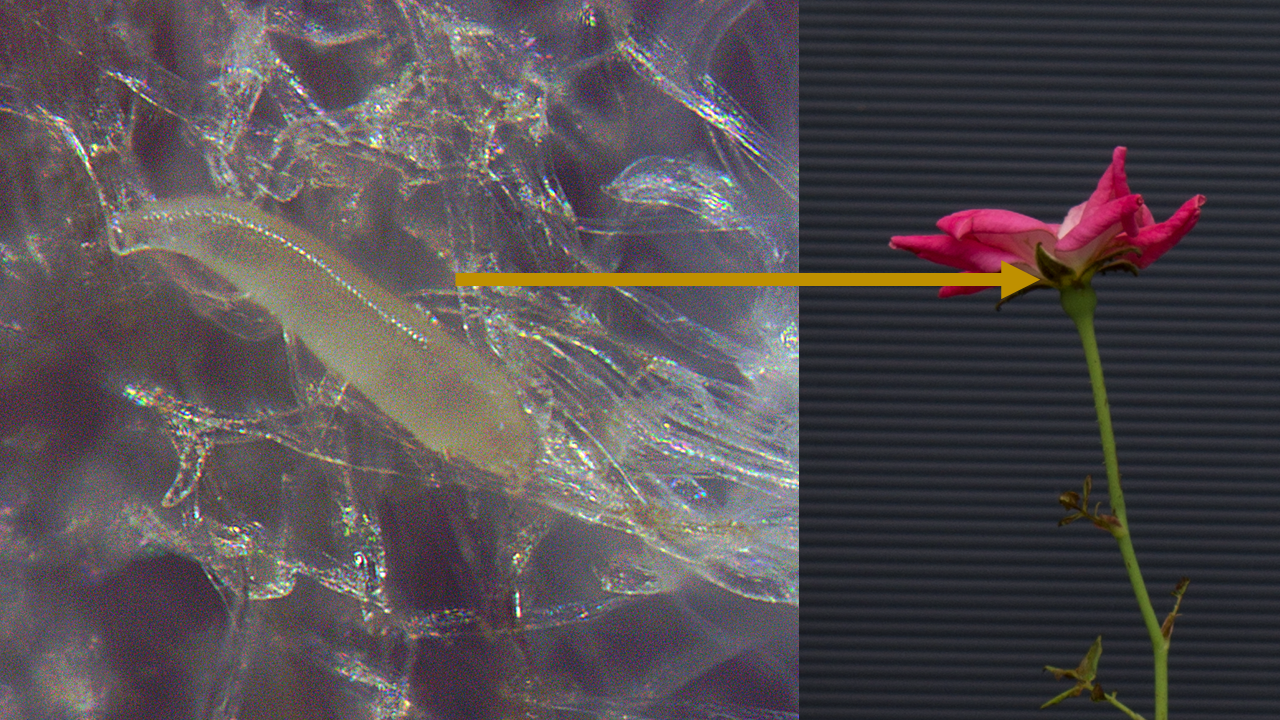
\includegraphics[width=0.8\linewidth]{figure/mite-pfruct-hide} \end{center}

  Figure 3: Illustration of the typical location of \emph{Phyllocoptes fructiphilus} on roses. \emph{P. fructiphilus} are difficult to manage with pesticides due to the protection offered by the sepals.

  \hypertarget{preds-litrev}{%
  \subsection{Phytoseiids mites: good options for biological control of mites?}\label{preds-litrev}}

  Many mites species have potential as a biological control (Gerson et al. 2003, Carrillo et al. 2015). Their efficiency as predators of pest species has been recognized for many years: One of the earliest recorded attempts at biological control was of a mite \emph{Tyroglyphus phylloxerae} (Riley \& Planchon), which was imported to France from the USA in an attempt to control the grape phylloxera, \emph{Daktulosphaira vitifoliae} (Fitch 1855) (Riley 1874, Dent 2000, Kirchmair et al. 2009). Although this early attempt was unsuccessful, several mite species have been successful in controlling pest species (Bellows Jr et al. 1996, Driesche et al. 2010). The most well-studied family of predatory mites used for biological control are the Phytoseiidae (Gerson et al. 2003, Farragut et al. 2010, Carrillo et al. 2015). The lifestyles of Phytoseiid mites are generally split into four categories based on feeding guilds as described in McMurtry and Croft (1997): Type I mites belong to the genus \emph{Phytoseiulus}, the only group considered to be specialists on spider mites from the genus \emph{Tetranychus}. These mites reproduce faster than other phytoseiid groups, but only thrive on spider mite prey. They also respond to kairomones emitted by \emph{Tetranychus} feeding (McMurtry and Croft 1997, Farragut et al. 2010). Type II phytoseiids are also heavily associated with \emph{Tetranychus}, including representatives from the genera \emph{Neoseiulus}, \emph{Galendromus}, and \emph{Typhlodromus}, but Type II mites also can feed on other mite groups, such as eriophyid, tydeid, and tarsonemid mites. They also can feed on pollen or plant exudates if necessary (McMurtry and Croft 1997, Farragut et al. 2010). Both Type I and Type II mites often live in the web colonies of their Tetranychid hosts, and have longer dorsal setae to avoid entanglement (McMurtry and Croft 1997, Farragut et al. 2010). Type III phytoseiids are considered to be generalists, and can grow and reproduce on a variety of different mite groups, including Eriophyoid, Tetranychoid, Tarsonemid and Acarid mites. They also feed on plant pollen, nectar, and insects such as whiteflies and thrips (McMurtry and Croft 1997, Farragut et al. 2010). The breadth of their feeding guild has encouraged their use in biological control programs (Farragut et al. 2010). Type III mites are more likely to feed on other mites of the same species, and require more prey for development than the specialist phytoseiid groups (McMurtry and Croft 1997, Farragut et al. 2010). Type III live on plants rather than in spider mite colonies, and accordingly have shorter dorsal setae. Type III mites will still feed opportunistically on \emph{Panonychus}, a groups of Tetranychid mites which produce less dense webbing (McMurtry and Croft 1997, Farragut et al. 2010). Lastly, Type IV mites belong to the genus \emph{Euseius}, which are polyphagous mites which primarily feed on pollen, although they will feed on other mites and small insects as well. They have short dorsal setae (McMurtry and Croft 1997, Farragut et al. 2010). Phytoseiid mites of all four types have been integrated successfully into various pest management programs. Many phytoseiids have been tested with various combinations of other biocontrol agents, such as predatory bugs and \emph{Beauveria bassiana} (Chow et al. 2010, Midthassel et al. 2016, Bouagga et al. 2018, Freitas et al. 2021), as well as certain pesticides (Trumble and Morse 1993, Nicetic et al. 2001, Fernández et al. 2017). Phytoseiid reproduction has been studied to develop methods for mass-rearing and releasing as biological control agents for thrips, whiteflies, spider mites (Tetranychidae), flat mites (Tenuipalpidae), scale insects and other pests (Gerson et al. 2003, Chen et al. 2006, Carrillo et al. 2011a, Carrillo and Peña 2011, Sarwar 2017, Knapp et al. 2018, Argolo et al. 2020). One of the more popular species of commercially-available predatory mite is \emph{Amblyseius swirskii} Athias-Henriot (Calvo et al. 2014). \emph{A. swirskii} is a Type III mite species (Farragut et al. 2010), which has been used successfully in agriculture for pest control of crop pests such as whiteflies (Bolckmans et al. 2005), spider mites (McMurtry et al. 1970), rust mites (Park et al. 2010, Onzo et al. 2012), broad mites (Tarsonemidae) (Lopez et al. 2016), and thrips (Wimmer et al. 2008). \emph{A. swirskii} tolerate shipping well (Lopez and Smith 2016) and are often sold packaged in vermiculite or in sachets with wheat bran which allows the mites to slowly release into the environment (Buitenhuis et al. 2014, Calvo et al. 2014). \emph{A. swirskii} can be reared on artificial diets (Nguyen et al. 2013), natural and supplemental pollen (Loughner et al. 2011, Park et al. 2011, Delisle et al. 2015) and/or other arthropods present in the environment even when the pest of concern is absent (Janssen and Sabelis 2015, Kumar et al. 2015). This allows \emph{A. swirskii} to be released periodically as a preventative measure instead of reacting to an outbreak (Kutuk and Yigit 2011). Volunteer and banker plants near cropping systems can also provide shelter for phytoseiids to live in (Smith and Papacek 1991, Coli et al. 1994, Xiao et al. 2012, Nunes et al. 2020). Type III phytoseiid mites are generally associated with plants (Farragut et al. 2010), and do not survive well without them (Jung and Croft 2000). Plant structures affect many aspects of a phytoseiid's life (Cortesero et al. 2000, Schmidt 2013), influencing dispersal (Buitenhuis et al. 2013, Lopez et al. 2016), as well as performance as predators (Cédola et al. 2001, Seelmann et al. 2007, Buitenhuis et al. 2013). For example, Type III phytoseiids prefer to live on `hairy' plants with dense trichomes, and will leave glabrous leaf surfaces (Loughner et al. 2010a, 2010b), often laying their eggs in the densest patches of plant hair, or the thick tufts of trichomes along axillary veins known as `domatia' on the underside of leaves (O'Dowd and Willson 1991, Walter 1992, 1996, Grostal and O'Dowd 1994, Agrawal and Karban 1997), possibly to avoid predation (Faraji et al. 2002). Predator-plant mutualisms also extend into the realm of chemical communications: many types of phytoseiids learn to associate their prey with Volatile Organic Compounds (VOCs) released when plants are injured by pests or infected with pathogens (Sabelis et al. 1999, Maeda and Takabayashi 2001, Boom et al. 2002, Boer and Dicke 2004a, 2004b, 2005). VOCs can repel (Moraes et al. 2001) attract (Nomikou et al. 2005, Gadino et al. 2012), encourage predation (Kessler and Baldwin 2001, Halitschke et al. 2007), or poison arthropods (Vancanneyt et al. 2001). Plant responses to herbivory differ between plant and predator species (Maeda and Liu 2006, Qualley and Dudareva 2008), underlining the importance of studying the specific interactions for each crop (Boom et al. 2004).
  \begin{center}\includegraphics[width=0.8\linewidth]{thesis_files/figure-latex/persim-1} \end{center}

  Figure 4: \emph{Phytoseiulus persimilis} are type I phytoseiid mites: specialists of spider mites from the genus \emph{Tetranychus} (McMurtry and Croft 1997, Farragut et al. 2010).

  \hypertarget{plantdef-litrev}{%
  \section{Induced plant defenses for biological control}\label{plantdef-litrev}}

  Plants are primarily sessile organisms which aren't able to run or hide, therefore undefended plants struggle to grow in the face of the constant threat of herbivory (Kessler et al. 2004). In order to combat being eaten, plants rely heavily on their ability to protect themselves \emph{in-situ}, via a myriad of different physical and chemical defenses (Walling 2000). These defenses are categorized as either constitutive defenses or induced defenses (Farmer 2016). Constitutive defenses are always `on,' being produced by the plant constantly, such as tannins and latex, while inducible defenses rely on some sort of signal before the plant will produce them. Physical defenses of herbivory includes spines, prickles, thorns, glandular trichomes, latex, sclereids, epicuticular wax, bark, thick cell walls, and compensatory growth to prevent tissue damage while increasing wear on herbivore mouthparts (Farmer 2016). In addition to these physical barriers to herbivory, plants are also efficient chemical factories which produce a bevy of secondary plant metabolites, including inhibitory proteins, enzymes, and toxins which reduce palatability of plant tissues, prevent uptake of essential amino acids, or kill the herbivore outright (Farmer 2016). It is hypothesized that inducible defenses must have evolved in response to threats that were sporadic in nature, but strong enough to necessitate a response (Edelstein-Keshet and Rausher 1989, Tollrain and Harvell 1999). The idea is that inducible defenses allow plants a type of cost-saving for their limited resources (Optimal Defense Theory, Steppuhn and Baldwin (2008); Adler and Karban (1994)), or to avoid damaging themselves with the compounds used (Steppuhn and Baldwin 2008). Otherwise, the evolution of constitutive defenses would seem to be a better option for plant defense (Karban and Myers 1989, Järemo et al. 1999). A corollary of the optimal defense theory is that inducible defenses should have cues that trigger dependably, accurately and be an effective deterrent once activated, so as to avoid opportunity costs (Berenbaum and Zangerl 1999, Järemo et al. 1999). Induced chemical defenses are thought to have an added benefit of being faster and less costly for plants to produce than other types of defense, such as developing spines or thicker cell walls (Berenbaum and Zangerl 1999, Järemo et al. 1999). Even so, chemical defenses still have drawbacks in allocation costs: plants investing energy into defenses are not using those resources for growth or reproduction (Berenbaum and Zangerl 1999). There are also probably genetic tradeoffs to keep inducible costs active rather than other essential plant functions, and there may be ecological compromises as well: adaptation to one form of defense may preclude the use of another (Berenbaum and Zangerl 1999). Another confounding factor with induced defenses occurs in the presence of specialist herbivores, many of which are especially adapted to overcoming a particular plant defense (Ehrlich and Raven 1964, Schoonhoven et al. 2005, Farmer 2016).

  \hypertarget{sar-litrev}{%
  \subsection{Can systemic acquired resistance be used to reduce mite herbivory?}\label{sar-litrev}}

  Järemo et al. (1999) considered the development of systemic responses to be more probable if plant defenses required larger doses for deterrence, and posited that localized responses to herbivory are benefit the plant when small amounts of initial damage are a reliable cues of larger damage to come. This framework readily considers the feeding activities of stylet feeders like mites, whose initial damages are minimal, but quickly accelerate due to mites' fast population growth rates. Accordingly, plants need to be responsive and accurate when identifying a threat before a defense can be mounted. Plants rely on pattern recognition receptors (PRRs) (Couto and Zipfel 2016), to detect pathogen-associated molecular patterns (PAMPS) (Boller and Felix 2009), and herbivore-associated molecular patterns (HAMPS) (Mithöfer and Boland 2008), molecules released from attacking pathogens and herbivores, respectively. These PRRs are part of innate plant immunity: PAMP-triggered immunity and effector-triggered immunity (ETI) (Chisholm et al. 2006, Jones and Dangl 2006). Plant cell-surface receptors detect common pathogen molecules, such as flagellar proteins, chitin and ergosterol. If activated PTI typically stops further invasion, by depositing callose at the site of infection, releasing reactive oxygen species (ROS), mitogen-activated protein kinases (MAPK, Howe and Jander (2008)), and inducing pathogen-responsive genes. If this first line of defense is surpassed, ETI has evolved to identify the proteins used to overcome PTI, by detecting pathogen effectors with the \emph{R} proteins encoded by the corresponding \emph{R}-genes in the plant (Boller and Felix 2009). One of the most well known effects of activating ETI is the hypersensitive response (HR), rapid localized cell death/necrosis at sites of infection. The HR also activates pathogensis-related (PR) genes and upregulates intercellular Salicylic Acid (SA), which converts to the VOC, Methyl Salicylate (MeSA), a signal which propagates resistance throughout the plant. The increased expression of PR genes primes the plant for long term resistance to future attack, via a process known as systemic acquired resistance (SAR) (Boller and Felix 2009, Vlot et al. 2009, Zhang et al. 2010). HAMPs work in a similar way to PAMPs, but instead of detecting molecular patterns associated with pathogens, they detect molecules associated with herbivores, such as arthropod oral secretions, eggs, pheromones, or other chemicals conserved across a wide range of arthropods (Mithöfer and Boland 2008). Plants respond to triggered HAMPS in similar ways: they also trigger ROS, MAPKs, and Ca\({^{2+}}\) influx at the site of injury (Vincent et al. 2017). Another important plant defense is the Jasmonic Acid (JA)-Ethylene (ET) signalling pathways. The JA/ET pathways are activated when JA upregulates in response to wounding and/or arthropod damage, and provides protection from herbivory as well as pathogen damage (Thaler et al. 2001, Farmer et al. 2003, Guo and Ecker 2004, Glazebrook 2005, Howe and Jander 2008). Plants can be primed directly through application of SA, MeSA or even synthetic chemical analogues, such as acibenzolar-S-methyl (ASM) to activate SAR (Conrath et al. 2006, Vlot et al. 2009, Zhang et al. 2010). SAR-induction increases levels of \textbeta-1,3-glucanase and chitinases (Bronner et al. 1991a, Ward et al. 1991), which prevent fungal disease development (Goy et al. 1992, Xue et al. 1998, Narusaka et al. 1999, Suo and Leung 2001). These proteins have potential for the biological control of pest mites: Bronner et al. (1991b); Bronner et al. (1991a) observed that feeding by the gall mite \emph{Aceria cladophthirus} (Nalepa) triggered the hypersensitive response on \emph{Solanum dulcamara}, producing chitinase and \textbeta-1,3-glucanase activity, which suggested that these may have a role in plant defenses against herbivores. Subsequent experiments by Westphal et al. (1991) also found that \emph{S. dulcamara}'s SAR response to \emph{A. cladophthirus} produced long lasting protection from subsequent colonization by more \emph{A. cladophthirus} or another eriophyid, \emph{Thamnacus solani} Boczek and Michalska, a rust mite. Unfortunately, later research by Westphal et al. (1992) demonstrated that these induced responses were not enough not protect the plant from \emph{Tetranychus urticae} Koch, but instead increased their fecundity. This type of interplay between induced defenses is common, and varies by plant species (Boom et al. 2004). The induction of SA and JA are known to exhibit negative cross-talk in some plant systems (Baldwin et al. 1997, Belliure et al. 2010, Thaler et al. 2012): Warabieda et al. (2020) observed that JA helped increase plant resistance to \emph{T. urticae}, but applying JA and ASM together was less effective than applying JA alone, due to SA interference with JA pathways. Other studies have found opposite effects: Favaro et al. (2019) reported reduced numbers of \emph{T. urticae} on strawberries post SA induction, and Khederi et al. (2018a) found that SA and JA induction was sufficient to control erineum forming \emph{Colomerus vitis} (Pagenstecher). This type of inconsistency is best explained by the results of Kant et al. (2007), which found examples of interspecific variation of \emph{T. urticae}'s ability to induce--and resist--JA defenses. Furthermore, there have been a number of cases where mites have been known to avoid or prevent upregulation of plant defenses entirely: Both \emph{T. urticae} and \emph{Aculops lycopersici} Massee, have been reported to suppress the JA pathways without relying on antagonistic cross-talk between the responses (Sarmento et al. 2011, Alba et al. 2014), instead by suppressing downstream accumulation of JA (Alba et al. 2014, Glas et al. 2014). Glas et al. (2014) observed that \emph{A. lycopersici} would still induces SA defenses, while an inducer species (Kant et al. 2007) of \emph{T. urticae} feeding on tomato (\emph{Solanum lycopersicum}) induces both JA and SA pathways, but when both mites were introduced to the same plant, the JA response plummeted and SA doubled (Glas et al. 2014). This caused \emph{A. lycopersici} populations to suffer while the \emph{T. urticae} populations benefited from \emph{A. lycopersici}'s reduction of JA (Glas et al. 2014). Vectors of plant pathogens create a similar struggle for their host plants by manipulating and suppressing the SA and JA/ET pathways for their mutual benefits (Agrawal and Karban 1999, Belliure et al. 2010). An example can be seen in the interactions of \emph{B. yothersi}, the vector of \emph{Citrus leprosis virus C} (CiLV-C): infection of \emph{Arabidopsis thaliana} and \emph{Citrus} spp. with CiLV-C induces SA and suppresses JA/ET pathways through crosstalk (Arena et al. 2016). A follow-up study of \emph{B. yothersi} feeding on \emph{A. thaliana} was similar in result: mite feeding triggered both SA and JA/ET pathways, but \emph{B. yothersi} reared on mutant \emph{A. thaliana} with no SA response had lower fecundity (Arena et al. 2018), suggesting that \emph{B. yothersi} rely on inducing SA to antagonize JA production. Inducing plant defenses can have negative consequences for the predators as well as the herbivores (Pappas et al. 2017): Ataide et al. (2016) observed that inducing a plant JA pathway reduced \emph{T. urticae} and \emph{T. evansi} mite performance, but also negatively affected ovophagy by \emph{Phytoseiulus longipes}, which ate fewer eggs from mites living on induced plants (Ataide et al. 2016), slowing their reproductive rate. It is also possible that the differences feeding methods between mite species is creating different defense responses, as has been seen in other arthropod groups (Zarate et al. 2006, Zhang et al. 2009, Arimura et al. 2011).

  \hypertarget{brevi-litrev}{%
  \section{\texorpdfstring{A second mite-plant-pathogen system: \emph{Brevipalpus californicus} and Orchid fleck virus}{A second mite-plant-pathogen system: Brevipalpus californicus and Orchid fleck virus}}\label{brevi-litrev}}

  The most important superfamily of herbivorous mites is the Tetranychoidea. The Tetranychoidea are comprised of 2,000 species divided into 5 families (Krantz 2009), two of which have economic significance, Tetranychidae--the spider mites--and Tenuipalpidae. Tenuipalpidae are known colloquially as the false spider mites, or flat mites due to their flattened character and superficial similarity to the Tetranychidae. In contrast to tetranychids, tenuipalpids do not spin webs and are considered to be a pest of reduced severity: Krantz (2009) places them as the `third most important family of phytophagous mites.' Flat mites are considered to be a tropical to subtropical group of mites (Gerson 2008), the majority of which are not of economic significance (Hoy 2011). Consequently, tenuipalpids have been studied much less than the Tetranychidae (Jeppson et al. 1975, Childers et al. 2003a, Gerson 2008), but flat mites from the genus \emph{Brevipalpus} have been gaining importance in recent years as vectors of plant viruses (Chagas et al. 2003, Childers et al. 2003c, Childers and Derrick 2003, Kitajima et al. 2003, Rodrigues et al. 2003, Kitajima et al. 2008, 2010, Childers and Rodrigues 2011, Melzer et al. 2013, Rodrigues and Childers 2013, Ramos-González et al. 2017, Chabi-Jesus et al. 2018, Dietzgen et al. 2018a). Another major pest of modern concern is \emph{Raoiella indica} (Hirst), a pest of palms (Arecaceae), ginger (Zingiberaceae), bananas (Musaceae), and bird of paradise plants (Strelitziaceae) (Jeppson et al. 1975, Etienne and Flechtmann 2006, Hoy 2011, Beard et al. 2012), which has been invading the Neotropics since their introduction to the Caribbean (Etienne and Flechtmann 2006, Rodrigues et al. 2007, Roda et al. 2008, Vásquez et al. 2008, Carrillo et al. 2011b, Dowling et al. 2011, Kane et al. 2012, Peña et al. 2012, Alcı́var et al. 2020, Escobar-Garcia and Andrade 2020, Ramı́rez et al. 2020, Rodrigues et al. 2020, Amaro et al. 2021). Flat mites are typically small (200 to 300 \si{\micro\metre}) red or green, and move slowly (Jeppson et al. 1975, Hoy 2011). Tenuipalpids feeding is typically restricted to a few hosts, and mites can usually be found on the underside of leaves, often along leaf veins or the midrib (Jeppson et al. 1975, Hoy 2011). Some species feed on grass, bark, flower heads, leaf sheaths, or form galls (Jeppson et al. 1975, Hoy 2011). Flat mites have egg, larva, protonymph, deutonymph and adult forms over an average of 3-4 weeks (Hoy 2011). A few species have only six legs as adults. Tenuipalpid mites can be difficult to classify correctly with light microscopy, due to distortions during mounting of characters used in species identification (Welbourn et al. 2003). Furthermore, flat mites are thelytokous parthenogenic: Males are seldom encountered, due to infections with the feminizing bacteria \emph{Candidatus} Cardinium (Cytophaga--Flavobacterium--Bacteroides phylum) Chigira and Miura (2005). This has caused some concern that some \emph{Brevipalpus} species are actually isofemale lines specialized on their specific hosts (Groot et al. 2005), an idea which is further complicated by the occurrence of cryptic species in these groups (Navia et al. 2013, Skoracka et al. 2015). Few methods of pest management have been reported from past reviews of tenuipalpids (Jeppson et al. 1975, Gerson 2008, Hoy 2011): a number of different mite predators have been tested for their efficacy, as well as the pathogenic fungi \emph{Hirsutella thompsonii} and \emph{Metarhizium anisopliae} (Rossi-Zalaf and Alves 2006, Gerson 2008). Zheng et al. (2012) tested the ability of water and phytoseiids to reduce populations of \emph{B. obovatus}. \emph{Beauveria bassiana} has been tested to control \emph{R. indica}, and is potentially compatible with the previously-tested phytoseiid species \emph{Amblyseius largoensis} and \emph{Typhlodromus ornatus} (Carrillo and Peña 2011, Freitas et al. 2021). Chemical applications are typically used to control tenuipalpids (Childers 1994), but some species have begun to develop chemical resistance to the more common applications (Campos and Omoto 2002, Rocha et al. 2021).
  \begin{center}\includegraphics[width=0.8\linewidth]{thesis_files/figure-latex/brevi_fungus-1} \end{center}

  Figure 5: a) Cryo-SEM image of Tenuipalpid mite infected with unidentified fungus, collected from \emph{Liriope muscari} b) detail of sporangia. Photo Credit: Dr.~Gary R. Bauchan, USDA-ARS, 2020

  One of the more cosmopolitan species of tenuipalpid is \emph{Brevipalpus californicus} (Banks). \emph{B. californicus} is a common pest with a large host range of agricultural and ornamental crops, including tea, orchids, citrus, cotton and tobacco (Jeppson et al. 1975, Hoy 2011). \emph{B. californicus} acts as the primary vector for Orchid fleck dichorhavirus (OFV), the type member for the genus \emph{Dichorhavirus}, family \emph{Rhabdoviridae}; a bacilliform, nuclear rhabdoviruses composed of two segments of single-stranded, negative-sense RNA which infects plants (Dietzgen et al. 2014, Walker et al. 2018, Amarasinghe et al. 2019). Dichorhaviruses are only known to be transmitted by mites in the genus \emph{Brevipalpus} (Dietzgen et al. 2014). Other members of this genus are: Citrus chlorotic spot virus, Citrus leprosis virus N, Clerodendrum chlorotic spot virus and Coffee ringspot virus (Dietzgen et al. 2018a). Many orchid genera are able to become infected with OFV (Kondo et al. 2006, 2006), as well as some Asparagaceae (Nolinoidaea) (Dietzgen et al. 2018a), and \emph{Citrus} plants (Rutaceae), where it causes leprosis-like symptoms (Bastianel et al. 2010, Roy et al. 2013, García-Escamilla et al. 2018). Mechanical transmission of OFV is possible under lab conditions to various Chenopodiaceae, Aizoaceae, Fabaceae, and Solanaceae (Chang et al. 1976, Kondo et al. 2003, Peng et al. 2013). \emph{B. californicus} has been collected from OFV-infected Nolinoidaea plants in Australia (Mei et al. 2016, Dietzgen et al. 2018b). \emph{B. californicus} was historically associated with cases of citrus leprosis disease of Florida and Texas prior to 1925, when the disease mysteriously disappeared from the US sometime during the 1960s (Knorr et al. 1968, Childers et al. 2003b). Later studies of herbarium specimens from this time period revealed this disease to be caused by a Dichorhavirus, distantly related to modern OFV strains (Kitajima et al. 2011, Hartung et al. 2015). Maeda (1998) found evidence that \emph{B. californicus} can transmit OFV in a persistent propagative manner, which means that the virus may replicate inside of its mite vector. OFV was first described infecting \emph{Cymbidium} orchids in Japan (Doi et al. 1977). Many countries have reported OFV and OFV-like rhabdoviruses infecting orchids worldwide (Kondo et al. 2003), including Asia: {[}China (Peng et al. 2017), Korea (Peng et al. 2013){]}, Africa: {[}South Africa (Blanchfield et al. 2001, Cook et al. 2019), North America: {[}The US (Blanchfield et al. 2001), (Bratsch et al. 2015){]}, South America: {[}Brazil Kitajima et al. (2001), Colombia (Kubo et al. 2009b), Costa Rica (Freitas-Astúa et al. 2002), Paraguay (Ramos-González et al. 2015), Europe: (Begtrup 1972), Germany (Petzold 1971, Lesemann and Doraiswamy 1975){]} and Oceania: (Australia Lesemann and Begtrup 1971, Lesemann and Doraiswamy 1975, Gibbs 2000), Fiji (Pearson et al. 1993), Vanuatu (Pearson et al. 1993){]}. The prevalence of OFV and its mite vector is thought to be associated with the importation of infected orchids (Dietzgen et al. 2018a). Orchids infected with OFV develop chlorotic/necrotic flecks on leaves and reduces plant vigor (Peng et al. 2013). Citrus infected with OFV develop chlorotic/necrotic bullseye lesions on leaves, fruits and bark (Roy et al. 2015, Ramos-González et al. 2017). Citrus-infecting strains of OFV have been encountered in Mexico (Roy et al. 2015) and recently in Hawaii (Ocenar 2020, Olmedo-Velarde et al. 2021), introduction of this virus is considered a threat to the billion dollar citriculture industries of the US.
  \begin{center}\includegraphics[width=0.8\linewidth]{thesis_files/figure-latex/oncidium_ofv-1} \end{center}

  Figure 6: \emph{Oncidium} orchid infected with Orchid fleck virus

  \hypertarget{first-report-of-phyllocoptes-fructiphilus-in-florida}{%
  \chapter{\texorpdfstring{First report of \emph{Phyllocoptes fructiphilus} in Florida}{First report of Phyllocoptes fructiphilus in Florida}}\label{first-report-of-phyllocoptes-fructiphilus-in-florida}}

  \includepdf[pages={-}]{pubs/pfruct-report.pdf}

  \hypertarget{survey}{%
  \chapter{\texorpdfstring{2. Objective 1: Survey for the invasive mite \emph{Phyllocoptes fructiphilus}, Rose Rosette Virus (RRV), and wild predatory mites in northern Florida}{2. Objective 1: Survey for the invasive mite Phyllocoptes fructiphilus, Rose Rosette Virus (RRV), and wild predatory mites in northern Florida}}\label{survey}}

  \hypertarget{survey-nfl}{%
  \section{\texorpdfstring{2.1 \emph{P. fructiphilus} detection in Northern Florida}{2.1 P. fructiphilus detection in Northern Florida}}\label{survey-nfl}}

  \hypertarget{problem-statement}{%
  \subsubsection{2.1.1 Problem Statement}\label{problem-statement}}

  Rose Rosette Virus (RRV), the casual agent of Rose Rosette Disease (RRD) and \emph{P. fructiphilus} Kiefer invaded the southeastern United States on the multiflora rose, \emph{R. multiflora} (Thunb) as it spread its range towards the coast (Amrine Jr 2002, Otero-Colina et al. 2018). RRD is present throughout the US, including Decatur County, GA, near the Florida border (\emph{Figure 7}), (EDDMapS 2019).
  \begin{center}
\includegraphics[width=0.8\linewidth]{figure/reed} \end{center}

  Figure 7: Map of the distribution of Rose Rosette Disease (RRD) in 2019 as reported from the Early Detection \& Distribution Mapping System maintained by the University of Georgia's Center for Invasive Species and Ecosystem Health. Areas in green are counties where RRD has been reported.

  In 2018, a group of researchers conducted a series of surveys for \emph{P. fructiphilus} and RRD in the southeastern United States (Solo 2018). They encountered \emph{P. fructiphilus} in Thomas County and Lowndes County, (\emph{Figure 8}), (Solo 2018), less than 20 miles from the northern border of Florida.
  \begin{center}
\includegraphics[width=0.8\linewidth]{figure/reed} \end{center}

  Figure 8: Distribution of \emph{Phyllocoptes fructiphilus} in the United States from Solo 2018. The black line circles represent areas where \emph{P. fructiphilus} have been found.

  Unfortunately, these surveys did not include Florida (see \emph{Figure 8}), (Solo 2018).

  In early 2019, a survey of predatory mites on roses found eriphyoid mites in samples obtained while surveying roses in Leon County, Florida. The mites were sent to the Florida Department of Agriculture and Consumer Services - Department of Plant Industry (FDACS-DPI) and were all identified as \emph{P. fructiphilus} by Dr.~Sam Bolton. To date, none of these roses have shown signs or symptoms of RDD and none of these plants have tested positive for presence of the virus.

  \hypertarget{first-report-of-phyllocoptes-fructiphilus-in-florida-1}{%
  \subsubsection{\texorpdfstring{2.1.2 First report of \emph{Phyllocoptes fructiphilus} in Florida}{2.1.2 First report of Phyllocoptes fructiphilus in Florida}}\label{first-report-of-phyllocoptes-fructiphilus-in-florida-1}}

  \emph{Phyllocoptes fructiphilus} is a microscopic plant-feeding eriophyid mite. Eriophyoid mites are very host specific (Oldfield 1996b, Skoracka et al. 2009) and \emph{P. fructiphilus} only feeds on plants in the genus \emph{Rosa} (Amrine Jr 1996). \emph{P. fructiphilus} is the vector of Rose Rosette Virus (RRV). RRV infection is commonly associated with the following symptoms: witches' brooms/rosetting, deformed flowers, increased prickle density, elongated shoots, reddened leaves and stems, and increased die-back
  which ultimately kills the rose host (Amrine Jr 1996). This disease is known as Rose Rosette Disease (RRD). and is the most serious disease of roses, creating millions of dollars of losses for growers. Rose Rosette Disease and the mite have invaded the southeastern united states as they followed the range expansion of the non-native \emph{Rosa multiflora} (Thunb) towards the coast (Amrine Jr 2002, Otero-Colina et al. 2018).

  In 2018 we began a series of surveys along the borders of northern Florida and southern Georgia

  A key part of \emph{P. fructiphilus} control is vector and disease monitoring. Previous surveys of the southeastern United States did not survey for \emph{P. fructiphilus} in Florida, but our own surveys have since detected \emph{P. fructiphilus} in northern Florida (unpublished). The virus was previously detected independently of the mite vector previously as well (Babu et al. 2014), so it is possible that \emph{P. fructiphilus} and/or RRV are present in other parts of the state. We propose a survey of mites on roses in Florida to estimate the distribution and populations of \emph{P. fructiphilus}, as well as to determinie RRV incidence. Doing so will provide us with insight into the epidemiology of \emph{P. fructiphilus} and RRV.

  An additional value of rose surveys will be detecting other mites present on roses: there are many species of predatory phytoseiid mites present in Florida with potential to control agricultural pests such as \emph{P. fructiphilus}. Native predatory mites sometimes have an advantage for bio-control because native mites have adapted to the environment where they will be released (Gerson 2014). Besides predatory mites, we also may encounter other alternative vectors of RRV or different mite species of concern which have not yet been reported in Florida.

  An IPM approach uses as many compatible methods of control as is possible. By investigating early detection, bio-control, and epidemiology, we hope to find methods to understand and control the spread of \emph{P. fructiphilius} and RRV.

  Cities with populations over 1,000 will be visited along this route and cuttings will be taken from various roses in each city. Rose species, symptoms and coordinates will be recorded to map out sites which have \emph{P. fructiphilus} or possibly Rose Rosette Disease.

  Rose tissue samples were taken from the periphery of various roses throughout Leon and Gadsden counties as well as surrounding regions. Rose tissues sampled included a mixture of flowers, fruits, buds and short lengths of rose cane, trimmed with bypass pruners and stored in quart sized plastic baggies. Pruners were sanitized with 70\% ethanol between cuts. Rose species and coordinates were recorded to map out sites which had predatory mites, \emph{P. fructiphilus}, or possibly RRD.

  Data will be collected monthly for two years:
  Sampling will be focused on the flowering tips of roses and include a mixture of flowers, fruits, buds, and short lengths of rose cane. Samples will be trimmed with bypass pruners which are routinely sanitized with 70\% ethanol between cuts. Samples will be stored in 500 mL wide-mouthed Polyethene bottles (Nalgene) with \textasciitilde10 mL of 95\% ethanol and shaken to coat the rose tissues for preservation.

  Samples will be processed using a washing method derived from Monfreda et al. (2007): The sampling bottles with ethanol and rose tissues will be vigorously shaken to dislodge any mites, then the ethanol poured over a stack of sieves with decreasing screen sizes: 180 μm, 53 μm, and 25 μm. The bottle and rose pieces will be further rinsed with 95\% ethanol over the sieve stack to dislodge any remaining mites. The 53 μm and 25 μm sieves will be processed separately; the 53 μm sieve retains larger mites while the 25 μm sieve retainS smaller mites, including \emph{P. fructiphilus}. The sieves will then be backwashed from the underside of their screen with a 95\% ethanol-filled wash bottle, starting from the highest point of a sieve and working to the bottom to flush any trapped debris and mites into a 50 mL centrifuge tube for storage and future observation. Samples will be observed under a dissecting microscope. Mites found among the plant debris will be siphoned off with a glass pipette and subsequently stored in micro-centrifuge containers with 95\% ethanol as a preservative. Select specimens from each sample will be made into prepared microscope slides. Mites will be cleared and mounted using the methods of Faraji and Bakker (2008): mites will be cleared and stained with Faraji and Bakker's modified clearing solution and heated on a hot plate until clear, then slide mounted with an iodine-modified Hoyer's slide mounting media (Hempstead Halide, Inc., Galveston, Texas, USA). Slides will be dried at 90 °C, then a ring of Red Glyptal (brand info) will be painted over the edges of the coverslip to seal the slide.

  A subset of 5 eriophyid samples each month will be selected for molecular testing using the methods described in Druciarek et al. (2019) to verify mite species identity and to insure no RRV presence within those mites. A subset of mite species also be confirmed with the acarologist, Dr.~Sam Bolton of the Florida Department of Agriculture and Consumer Services (FDACS) to ensure accuracy.

  If any plants show symptoms of RRD, samples will be taken and tested by the Plant Disease Diagnostic Clinic at the NFREC using the methods of Babu et al. (2016), Babu et al. (2017a), and/or Babu et al. (2017b).

  Rose samples were processed using a washing method derived from Monfreda et al. (2007): cut roses were soaked in a 500 mL beaker with a solution of 1:1 bleach:water with few drops of dishwasher detergent. The solution was stirred vigorously with a glass rod to dislodge any mites. This solution was then poured over a stack of sieves with decreasing screen sizes: 180 \si{\micro\metre}, 53 \si{\micro\metre} and 25 \si{\micro\metre}.
  The beaker and rose pieces were further rinsed with tap water over the sieve stack to knock off any remaining mites. The 25 \si{\micro\metre} sieve screen traps mites which are the size of \emph{P. fructiphilus}. This sieve was then backwashed from the underside of the screen with a water-filled wash bottle, starting from the highest point of the sieve and working to the bottom of the sieve to flush the trapped debris into a 50 ml centrifuge tube for storage and future observation. Samples were observed under a dissecting microscope. Mites found among the plant debris were siphoned off with a glass pipette and subsequently stored in micro-centrifuge containers filled with 95\% ethanol as a preservative. Select specimens were mounted directly into Hoyer's slide mountant (Hempstead Halide, Inc.~Galveston, TX), dried at 90°C, then ringed with nail polish.

  On February 14, 2019, we found a total of 42 eriophyid mites from six samples obtained while surveying roses in Leon County, Florida. (see \emph{Figure 9A}) The mites were sent to the Florida Department of Agriculture and Consumer Services - Department of Plant Industry (FDACS-DPI) and were all identified as \emph{P. fructiphilus} using the keys provided in (Baker et al. 1996). The roses did not show signs or symptoms of RDD. These roses were tested for RRV with RT-qPCR and Reverse Transcription Recombinase Polymerase Amplification (RT-RPA) (Babu et al. 2016, 2017a). However, none of the plants infested with \emph{P. fructiphilus} were positive for RRV.

  On July 16th we conducted an additional survey of 33 roses near the initial site of discovery, including the rose sites where P. fructiphilus were originally detected. (see \emph{Figure 9B}), Each sample contained more than 50 eriophyid mites, with some samples containing over 300 mites. We compared the samples collected during February and July with a paired t-test and we found a significant increase in \emph{P. fructiphilus} population between the two sampling dates: p-value = 0.001, α = 0.05, df = 4. A subsample of these mites were slide mounted and subsequently confirmed as \emph{P. fructiphilus}. Additional rose samples were tested for RRV by RT-qPCR, but no virus was detected.

  This is the first record for \emph{P. fructiphilus} in Florida. More importantly, RRV is currently not established in Florida. None of the mite-infested roses had symptoms of RRD and none were positive for RRV. However, the presence of \emph{P. fructiphilus}, along with past detections of RRV in Florida warrants increased monitoring for the mite and virus in Florida. There is a critical need to develop methods to manage \emph{P. fructiphilus} and RRV, or the US rose industry stands to lose millions on mite control.
  \begin{center}
\includegraphics[width=0.8\linewidth]{figure/reed} \end{center}

  Figure 9: Presence of \emph{Phyllocoptes fructiphilus} in Leon County, Florida in (A) Feburary 2019 and (B) July 2019. Orange dots indicate sites sampled which had \emph{P. fructiphilus}. Gray areas indicate previously surveyed areas where no \emph{P. fructiphilus} were found.
  \begin{center}
\includegraphics[width=0.8\linewidth]{figure/reed} \end{center}

  Figure 10: Log number of \emph{Phyllocoptes fructiphilus} per rose sample. Samples were taken from sites in Leon County, Florida on February 14 and July 16th, 2019. Asterisks represent significant differences as calculated by pairwise t-tests of the 5 sites tested for \emph{P. fructiphilus} during both months. a = 0.05, p-value = 0.001.

  \hypertarget{proposal-a-series-of-surveys-for-p.-fructiphilus-and-rose-rosette-disease-in-northern-florida}{%
  \subsubsection{\texorpdfstring{2.1.3 Proposal: a series of surveys for \emph{P. fructiphilus} and Rose Rosette Disease in northern Florida}{2.1.3 Proposal: a series of surveys for P. fructiphilus and Rose Rosette Disease in northern Florida}}\label{proposal-a-series-of-surveys-for-p.-fructiphilus-and-rose-rosette-disease-in-northern-florida}}

  A key part of controlling the spread of \emph{P. fructiphilus} is mite and disease monitoring. We propose an expanded survey of mites on roses in Florida to estimate the populations and distribution of \emph{P. fructiphilus}, as well as to detect if Rose Rosette Disease is present. Doing so will provide us with insight into the patterns of how \emph{P. fructiphilus} and RRD spread.

  An additional value of rose surveys will be detecting other mites present on roses: there are many species of mites present in Florida with potential to control agricultural pests such as \emph{P. fructiphilus}. Native predatory mites sometimes have an advantage for bio-control because native mites have adapted to the environment where they will be released. Besides predatory mites, we also may encounter other vectors of RRD or different mite species of concern which have not yet been reported in Florida.

  \hypertarget{materials-methods}{%
  \subsubsection{2.1.4 Materials \& Methods}\label{materials-methods}}

  A survey of roses in the landscape was conducted following a transect of northern Florida from west to east, Pensacola to Jacksonville. Cities with populations over 1,000 were visited along this route and cuttings were taken from various roses in each city. Rose cultivar/species, sun exposure and GPS coordinates were recorded to map out sites which had predatory mites, eriophyid mites, or possibly symptoms of Rose Rosette Disease. Rose tissue samples were taken from the periphery of various roses in the landscape; sampling was focused on the flowering tips of roses and included a mixture of flowers, fruits, buds, and short lengths of rose cane. Samples were trimmed with bypass pruners which were routinely sanitized with 70\% ethanol between cuts. Samples were stored in 500 mL Nalgene™ Wide-Mouth Polypropylene Copolymer bottles (ThermoFisher Scientific, Waltham, MA, USA) with \textasciitilde10 mL of 95\% ethanol. The rose samples then were gently shaken to coat the rose tissues sampled with ethanol. Doing so made sure that the sampled mites were killed and acted to preserve both mites and rose tissues until samples could be processed further and checked for mites.

  Samples were processed using a washing method derived from Monfreda et al. (2007) used to detect eriphyoid mites such as \emph{P. fructiphilius}: The sampling bottles with ethanol and rose tissues were vigorously shaken to dislodge any mites, then the ethanol in the container was poured over a stack of sieves with decreasing screen sizes: 180 \si{\micro\metre}, 53 \si{\micro\metre}, and 25 \si{\micro\metre}. The bottle and rose pieces were then further rinsed with 95\% ethanol over the sieve stack to dislodge any remaining mites. The 53 \si{\micro\metre} and 25 \si{\micro\metre} sieves were processed separately; the 53 \si{\micro\metre} sieve retained larger mites while the 25 \si{\micro\metre} sieve retained smaller mites, including \emph{P. fructiphilus}. The sieves were then backwashed from the underside of their screen with a 95\% ethanol-filled wash bottle, starting from the highest point of a sieve and working to the bottom to flush any trapped debris and mites into a 50 mL centrifuge tube for storage and future observations.

  The ethanol solutions of mites and plant debris were allowed to settle until excess ethanol could be siphoned off, allowing us to then pour this concentrated plant-mite mixture into a thin, small petri dishes to be observed under a dissecting microscope. Mites found among the plant debris were counted, then siphoned off with a glass pipette and subsequently stored in micro-centrifuge containers with 95\% ethanol as a preservative. 5-10 specimens from each sample were made into prepared microscope slides: Mites were cleared and mounted using the methods of Faraji and Bakker (2008): mites were simultaneously cleared and stained with Faraji and Bakker's modified clearing solution and heated on a hot plate until the specimens were clear. Subsequently these mites were moved with an eyelash tool into an iodine-modified Hoyer's slide mounting media (Hempstead Halide®, Inc., Galveston, Texas, USA), underneath a 12 mm glass coverslip. The prepared slide was then dried at 90 °C before sealing the slide by painting a ring of alkyd insulating enamel (Red Glyptal® 1201, Chelsea, MA, USA) over the edges of the coverslip to seal the slide, to protect it from damage by air incursion and moisture. These slides could then be observed under a compound microscope with phase-contrast objectives to identify the mite families and species if necessary.

  A subset of up to 10 samples per site will be selected for molecular testing using the methods described in Druciarek et al. (2019) for determining mite species identity and RRV presence within those mites.

  After mite quantities and species were recorded, a representative sample of eriophyoids putatively identified as \emph{Phyllocoptes fructiphilus} had their identity verified with the acarologist, Dr.~Sam Bolton of the Florida Department of Agriculture and Consumer Services, Division of Plant Industry (FDACS-DPI) to ensure accuracy.

  Roses which appeared to show symptoms of Rose Rosette Disease, or which had populations of \emph{P. fructiphilus} present were tested by the Plant Disease Diagnostic Clinic at the NFREC. Plant tissues were tested for Rose rosette virus by Dr.~Fanny Iriarte using the currently accepted molecular methods described in Babu et al. (2016), Babu et al. (2017a), and/or Babu et al. (2017b).

  \hypertarget{potential-benefits}{%
  \subsubsection{2.1.5 Potential benefits}\label{potential-benefits}}

  Florida is the largest producer of roses with a total value exceeding \$30 million, and stands to lose millions of dollars if RRD and \emph{P. fructiphilus} become established. At this point, it is critical to develop action plans to control eriophyid mites on roses. By conducting this survey and finding \emph{P. fructiphilus} and RRD in the Florida landscape, we can determine the severity of the situation and inform growers who are in areas of greater risk. Informed nurseries can then take actions to protect their ornamentals from mite infestation, and can be vigilant for RRD symptoms.

  \hypertarget{expected-outcomes}{%
  \subsubsection{2.1.6 Expected outcomes}\label{expected-outcomes}}

  Potential outcomes of the mite surveys are fourfold:
  \begin{itemize}
  \item
    Detect the range of \emph{Phyllcoptes fructiphilus} and/or Rose Rosette Disease in northern Florida
  \item
    Identify native predatory mites with bio-control potential
  \item
    Identify other possible vectors of RRD
  \item
    Detect other mite species of concern on Florida roses
  \end{itemize}
  Our results will help identify areas with greater disease risk for \emph{P. fructiphilus} and/or RRV.

  Overall, we believe that the various objectives of this proposal will answer fundamental questions regarding the potential spread of \emph{Phyllocoptes fructiphilus} and Rose Rosette Disease (RRD) in Florida. RRD has been found without the mite, and now we may have found the mite without the pathogen at different parts of the year. This suggests that \emph{P. fructiphilus} and RRD have potential to become established in Florida. This research would be a first step in the development of preventative measures against RRD in Florida and will have direct practical outcomes that could be implemented in the short term to protect Florida production of roses.

  \hypertarget{swirskii}{%
  \chapter{\texorpdfstring{3. Objective 2: Potential of the predatory mite \emph{Amblyseius swirskii} to control \emph{Phyllocoptes fructiphilus}}{3. Objective 2: Potential of the predatory mite Amblyseius swirskii to control Phyllocoptes fructiphilus}}\label{swirskii}}

  \hypertarget{swirskii-roses}{%
  \section{\texorpdfstring{3.1 \emph{A. swirskii} attraction to RRV-infected roses}{3.1 A. swirskii attraction to RRV-infected roses}}\label{swirskii-roses}}

  Rose Rosette Virus (RRV), the casual agent of Rose Rosette Disease (RRD) and \emph{P. fructiphilus} Kiefer invaded the southeastern United States on the multiflora rose, \emph{R. multiflora} (Thunb) as it spread its range towards the coast (Amrine Jr 2002, Otero-Colina et al. 2018). RRD is present throughout the US, including Decatur County, GA, near the Florida border (\emph{Figure 7}), (EDDMapS 2019).

  Rose Rosette Virus (genus \emph{Emaraviridae}) is the most devastating disease of roses. Rose Rosette Virus creates witches' brooms, rosetting, deforms flowers, increases prickle density, elongates shoots, reddens of plant tissues, causes dieback and ultimately plant death. Rose Rosette Virus is spread by a microscopic eriophyid mite known as \emph{Phyllocoptes fructiphilus} Keifer (Trombidiformes: Eriophyidae). Few management options are available: Current mite control is achieved by removing infected roses and frequent pesticide applications. Growers are interested in alternative and less expensive management options to combat \emph{P. fructiphilus} and Rose Rosette Virus. Predatory mites have potential to fulfill this need: Mites from the family Phytoseiidae are being investigated as biocontrol agents for the management of \emph{P. fructiphilus}. Preliminary data suggest that the phytoseiid mite \emph{Amblyseius swirskii} Athias-Henriot (Mesostigmata: Phytoseiidae) orients itself towards volatiles of Rose Rosette-infected roses. This attraction may have synergistic effects for \emph{P. fructiphilus} control. \emph{A. swirskii} and three other commercially-available phytoseiid mites will be tested in olfactometer choice tests to identify specific volatile compounds which may be causing this behavior. Findings will help to develop chemical lures and promote depredation on \emph{P. fructiphilus} in Rose Rosette-infected roses. This research will contribute a biocontrol option for the management of \emph{P. fructiphilus} in southern Georgia and northern Florida.

  \hypertarget{statement-of-problem-rationale-and-justification}{%
  \subsubsection{Statement of Problem, Rationale and Justification}\label{statement-of-problem-rationale-and-justification}}

  The purpose of this project is to investigate the predatory persistence of four commercially-available mites for management of \emph{P. fructiphilus} and RRV in southern Georgia and northern Florida. Specifically, this project will determine which compounds released from Rose Rosette Virus (RRV) infected Double Knock Out® roses encourage recruitment, lengthen search time or improve depredation of phytoseiid mites on \emph{Phyllocoptes fructiphilus} Keifer (Trombidiformes: Eriophyidae).

  Phytoseiid mites have no eyes, instead relying on plant volatiles such as Methyl Salicylate to guide them to their prey (Boer and Dicke 2004a). Methyl Salicylate is also released when a plant is attacked by herbivores or pathogens (Shulaev et al. 1997, Boer and Dicke 2004a), so when preliminary tests with \emph{A. swirskii} showed attraction to RRV-infected roses, coupled Gas Chromatography-Mass Spectroscopy analysis was expected to reveal high levels of Methyl Salicylate. Contrary to expectation, RRV-infected roses had low levels of Methyl Salicylate compared to healthy plants. This suggests that phytoseiid attraction may be attributed to volatiles besides Methyl Salicylate. This is important because such volatiles may be used to lure phytoseiids to eriophyid-infested areas, encouraging feeding and enhancing pest control (Boer and Dicke 2004a, 2004b). Understanding which volatiles are responsible for phytoseiid attraction to RRV-infected roses will provide preliminary research which impacts management options for \emph{P. fructiphilus} in southern Georgia/northern Florida as well as other \emph{P. fructiphilus} \& RRV-infested regions.

  \hypertarget{project-relevance-to-sustainable-agriculture}{%
  \subsubsection{Project Relevance to Sustainable Agriculture}\label{project-relevance-to-sustainable-agriculture}}

  This project will contribute to agricultural sustainability by developing biological-control management practices for the control of Rose Rosette Virus (RRV). Understanding how predatory mites interact with volatiles in their environment will add value to biocontrol by encouraging predatory persistence, luring mites to areas where their prey is present and increasing prey-seeking behaviors (Boer and Dicke 2004a, 2004b). Chemical lures such as Methyl Salicylate can also encourage local recruitment of nearby mites and other natural predators (Boer and Dicke 2004a, 2004b), which can contribute to control of other pests of roses. Predatory mites are not environmentally-damaging or a health concern. Phytoseiid mites are compatible with some pesticides and other biocontrol methods, and feed on many different agricultural pests as well, so they can integrate well with existing pest management programs. Developing a biocontrol option for RRV can also increase profitability for rose growers not only by reducing losses from RRV-infection, but by reducing the number of pesticides which need to be applied. Reducing grower's reliance on pesticides has multiple benefits, promoting the health and safety of growers as well as protecting the environment. Reducing pesticide usage can also prevent \emph{P. fructiphilus} from developing pesticide resistance and decrease risks for pollinators which frequent roses. Predatory mites are low-low-maintenance to rear and deploy and subsist in the environment without decreasing sustainability in other areas. Overall, predatory mites represent great value for sustainable agriculture.

  \hypertarget{objectives}{%
  \subsubsection{Objectives}\label{objectives}}
  \begin{enumerate}
  \def\labelenumi{\arabic{enumi}.}
  \tightlist
  \item
    Determine which of four commercially-available phytoseiid mites (\emph{Amblyseius swirskii} Athias-Henriot, \emph{Neoseiulus californicus} (McGregor), \emph{Neoseiulus cucumeris} (Oudemans), and \emph{Neoseiulus fallacis} (Garman)) demonstrate attraction to Rose Rosette Virus (RRV)-infected roses
  \item
    Determine which volatiles are causing this attraction with Gas Chromatography-Mass Spectrometry
  \item
    Develop synthetic blends of the attractive volatiles and compare them to RRV-infected rose volatiles and the control (filtered air).
  \item
    Release the mites with lures on roses in Griffin, Georgia and observe depredation on \emph{P. fructiphilus} and recruitment of local mite species
  \item
    Report which of the mite spp. demonstrate significantly higher depredation of \emph{P. fructiphilus}
  \item
    Report the efficacy of lure deployment
  \end{enumerate}
  \hypertarget{approach-and-methods}{%
  \subsubsection{Approach and Methods}\label{approach-and-methods}}

  A brief description of the methods to be used for each objective, numbered according to their corresponding objective. There must be a direct relationship between the approach and methods and the project relevance to sustainable agriculture. Approach and Methods is limited to no more than 1000 words.
  \begin{enumerate}
  \def\labelenumi{\arabic{enumi}.}
  \tightlist
  \item
    Count the number of mites which choose to walk towards volatiles from RRV-infected roses rather than the control (untreated filtered air) with two-arm olfactometer assays analyzed using (\textbf{appropiatestaticalmethod?}) tests. Mites which significantly choose RRV-infected rose volatiles over the control will be considered ``responsive'' and used for further assays.
  \item
    Measure amounts of headspace volatiles extracted from both RRV-infected and uninfected roses. Paired Gas Chromatography-Mass Spectrometry will measure the quantity and determine the types of volatiles released using (\textbf{appropiatestaticalmethod?}) tests.
  \item
    Count the number of responsive mites which choose to walk towards synthetic volatile blends rather than the control (untreated filtered air) with two-arm olfactometer assays analyzed using (\textbf{appropiatestaticalmethod?}).
  \item
    Count the number of responsive mites which choose to walk towards synthetic volatile blends rather than volatiles from RRV-infected roses or controls (untreated filtered air) with four-arm olfactometer assays analyzed using (\textbf{appropiatestaticalmethod?}).
  \item
    Compare populations of \emph{P. fructiphilus}, phytoseiid mites and RRV infection in field trials in Griffin, Georgia with randomized block experiments comparing synthetic lures to controls without lures and analyzing data with (\textbf{appropiatestaticalmethod?}).
  \end{enumerate}
  \hypertarget{problem-statement-1}{%
  \subsubsection{3.1.1 Problem Statement}\label{problem-statement-1}}

  Salicylic Acid plays a role in activating a plant's immune system and helps protect the plant from pests, bacteria, fungus or viruses (Gozzo and Faoro 2013). We are collaborating with the University of Georgia to test how activating plant defensive compounds might protect roses from \emph{P. fructiphilus} and/or RRD. We applied Acibenzolar-S-methyl (ASM), a chemical which works like Salicylic Acid to activate plant defenses (Ziadi et al. 2001, Tripathi et al. 2010) at a high and a low rate, as well as a miticide and water as controls. These data suggest that activated plant defenses may work to control \emph{P. fructiphilus}.

  \hypertarget{preliminary-data}{%
  \subsubsection{3.1.2 Preliminary Data}\label{preliminary-data}}

  Predatory mites do not feed on the plants they live on, so they shouldn't be harmed by activated plant defensive compounds. In natural systems, predatory mites learn to follow plant defensive chemicals to find their prey (Boer and Dicke 2004a). This suggests that combining ASM-activated plant defenses with predatory mites may enhance the ability of predatory mites to find their prey, but this combination hasn't been tested yet.

  Preliminary tests with \emph{A. swirskii} show attraction towards compounds from RRV-infected roses. The lab has tested some of these compounds with Y-tube choice tests to determine their role in attracting \emph{A. swirskii} to the infected roses. Other chemicals remain to be tested. Understanding which chemicals are responsible for attracting \emph{A. swirskii} to RRV-infected roses is a preliminary part of determining if \emph{A. swirskii} will search for \emph{P. fructiphilus} when on a rose.
  \begin{center}
\includegraphics[width=0.8\linewidth]{figure/reed} \end{center}

  Figure 11: \emph{Amblyseius swirskii} attraction to healthy and Rose Rosette Virus-infected Pink Double Knock Out® roses. Asterisks represent significant differences as calculated by χ-squared contingency table tests for given probabilities. N.S. = not significant. RRV-infected vs Healthy Rose: χ-squared = 9.33, df = 1, a = 0.05, p-value = 0.002. Filtered Air vs Healthy Rose: χ-squared = 0.47, df = 1, a = 0.05, p-value = 0.4913.

  \hypertarget{swirskii-trials}{%
  \section{3.2 Volatile changes in Rose Rosette Virus-infected Plants Treated with Acibenzolar-S-Methyl, a functional analog of Salicylic Acid}\label{swirskii-trials}}

  \hypertarget{problem-statement-2}{%
  \subsubsection{3.2.1 Problem Statement}\label{problem-statement-2}}

  Some mites orient themselves towards volatiles of their prey or the host plant of their prey. We intend to investigate differences between RRV-infected and uninfected Pink Double Knock Out® roses and their volatiles, as well as the effects of SAR-induction on rose volatiles. The results will help inform future assays involving predatory mites and their \emph{P. fructiphilus}-seeking behaviors in relation to rose RRV-infection status and the use of SAR-inducers for biological control.

  \hypertarget{materials-methods-1}{%
  \subsubsection{3.2.2 Materials \& Methods}\label{materials-methods-1}}

  We plan on collecting plant volatiles from Double Knock Out® roses and comparing the differences between RRV-infected and uninfected roses, using a push-pull volatile collection system as illustrated in \emph{Figure 12}. Filtered air fills an oven bag sealed over rose canes to trap leaf volatiles. Volatiles are then drawn through a clean collection filter by a vaccuum. The chemicals on the filter are eluted with 150 ul of dichloromethane, then 5 ul of nonyl acetate are added as an internal standard to the extraction. The extractions then are injected into a GC-MS and their spectra are analyzed. Compounds are identified by comparison to mass spectra databases as well as synthetic standards for confirmation.

  Treatments will be the following:
  \begin{enumerate}
  \def\labelenumi{\arabic{enumi}.}
  \tightlist
  \item
    Uninfected Pink Double Knock Out® roses
  \item
    RRD infected Pink Double Knock Out® roses
  \item
    SAR-induced uninfected Pink Double Knock Out® roses
  \item
    SAR-induced RRD-infected Pink Double Knock Out® roses
  \end{enumerate}
  A group of 20 plants will be isolated. Volatiles from the 20 plants will be collected as a baseline (already collected). Then half of the plants will be SAR inducted by bi-weekly spray applications of Acibenzolar-S-Methyl. Subsequently half of the remaining plants (5 control and 5 SAR-induced plants) will be grafted with RRV-infected buds to innoculate them with the virus (Doudrick et al. 1987). Volatiles will be collected bi-monthly following SAR-induction and RRV application.
  \begin{center}\includegraphics[width=0.8\linewidth]{thesis_files/figure-latex/test-vols-1} \end{center}

  Figure 13: Volatile collection system for rose headspace sampling. An inert nylon bag is placed around the canes of interest, an air inlet is inserted and sealed at the base with a zip-tie to form a relatively air-tight seal around the base of the rose canes. Once the bag begins to inflate, a small hole is cut in the corner of the bag and a filter inserted and sealed with a zip-tie to form a second seal. The exterior end of the filter is attached to a vacuum airline set to allow for constant static pressure on the bag from inflation. The rose is then left for 24 hours, the filter is eluted with Dichloromethane into a gas chromatography vial, 1 ul of Nonyl Acetate is added as an internal standard, and then the sample is processed using a coupled Gas Chromatography - Mass Spectrometer (GC-MS) for chemical identification.

  \hypertarget{potential-benefits-1}{%
  \subsubsection{3.2.3 Potential benefits}\label{potential-benefits-1}}

  By determining which chemicals change during infection or with SAR-induction, we can gain insight into the physiological changes occuring during RRV-infection and SAR-induction in roses. Testing headspace volatiles can also give us insight into what VOCs predators like \emph{A. swirskii} may encounter on infected or SAR-induced roses.

  \hypertarget{expected-outcomes-1}{%
  \subsubsection{3.2.4 Expected outcomes}\label{expected-outcomes-1}}
  \begin{itemize}
  \item
    Determine which headspace VOCs are different between RRV-infected and healthy roses
  \item
    Determine what effects SAR-induction has on RRV-infected and healthy roses
  \item
    Creates a starting point for volatile testing for future olfactometer studies with \emph{A. swirskii}
  \end{itemize}
  Knowing which VOCs affect the host-seeking abilities of a predatory mite like \emph{A. swirskii} is part of preliminary work for determining the compatibility of \emph{A. swirskii} as a predator of \emph{P. fructiphilus}.

  \hypertarget{proposal-a-series-of-behavioral-tests-to-determine-which-compounds-from-rrv-infected-pink-double-knock-out-roses-are-attractive-to-a.-swirskii}{%
  \subsubsection{\texorpdfstring{3.3.1 Proposal: a series of behavioral tests to determine which compounds from RRV-infected Pink Double Knock Out® roses are attractive to \emph{A. swirskii}}{3.3.1 Proposal: a series of behavioral tests to determine which compounds from RRV-infected Pink Double Knock Out® roses are attractive to A. swirskii}}\label{proposal-a-series-of-behavioral-tests-to-determine-which-compounds-from-rrv-infected-pink-double-knock-out-roses-are-attractive-to-a.-swirskii}}

  We propose observing the behavior of \emph{A. swirskii} with Y-tube choice tests to test \emph{A. swirskii}'s potential to control \emph{P. fructiphilus}.

  \hypertarget{materials-methods-2}{%
  \subsubsection{3.3.2 Materials \& Methods}\label{materials-methods-2}}

  \emph{Amblyseius swirskii} Athias-Henriot will be reared according to procedures adapted from Sarwar (2017): \emph{A. swirskii} mites will be reared in growth chambers set at 25 °C with 70\% RH and 16:8 hours light:dark. Colonies will be kept in vermiculite-filled plastic containers, which will be suspended on plastic pylons in a moat of water with a surfactant to break the surface tension, preventing mite escape. Colonies will be fed every 2 days with bee pollen.
  \begin{enumerate}
  \def\labelenumi{\arabic{enumi}.}
  \item
    We will analyze differences in headspace VOCs extracted from both RRV-infected and uninfected roses using paired Gas Chromatography-Mass Spectrometry and preform a Principal Component Analysis to determine which compounds are good candidates for testing \emph{A. swirskii} attraction.
  \item
    We will record the reponses of \emph{A. swirkii} mites with two-arm olfactometer assays to determine the attractiveness to the selected compounds and analyze the results using χ-squared tests.
  \item
    If there are significant differences in \emph{A. swirskii} attraction towards single compounds or blends with Y-tube assays, we will preform a series of tests with four-arm olfactometer assays to compare \emph{A. swirskii} choices between different attractive compounds.
  \end{enumerate}
  \hypertarget{potential-benefits-2}{%
  \subsubsection{3.3.3 Potential benefits}\label{potential-benefits-2}}

  \emph{A. swirskii} are compatible with some pesticides and existing bio-control methods. \emph{A. swirskii} feed on other pests as well, so they can integrate with existing pest management programs. Developing a bio-control option for RRD can increase profitability for rose growers, reduces losses from RRV-infection, and reduce the number of pesticide applications required. Reduced reliance on pesticides promotes the health and safety of growers as well as protecting the environment. Reducing pesticide usage can also prevent \emph{P. fructiphilus} from developing pesticide resistance and decrease risks for pollinators which frequent roses. Predatory mites are low-maintenance to rear and deploy. Mites subsist in the environment without decreasing sustainability in other areas. Overall, predatory mites represent great value for sustainable agriculture.
  \begin{center}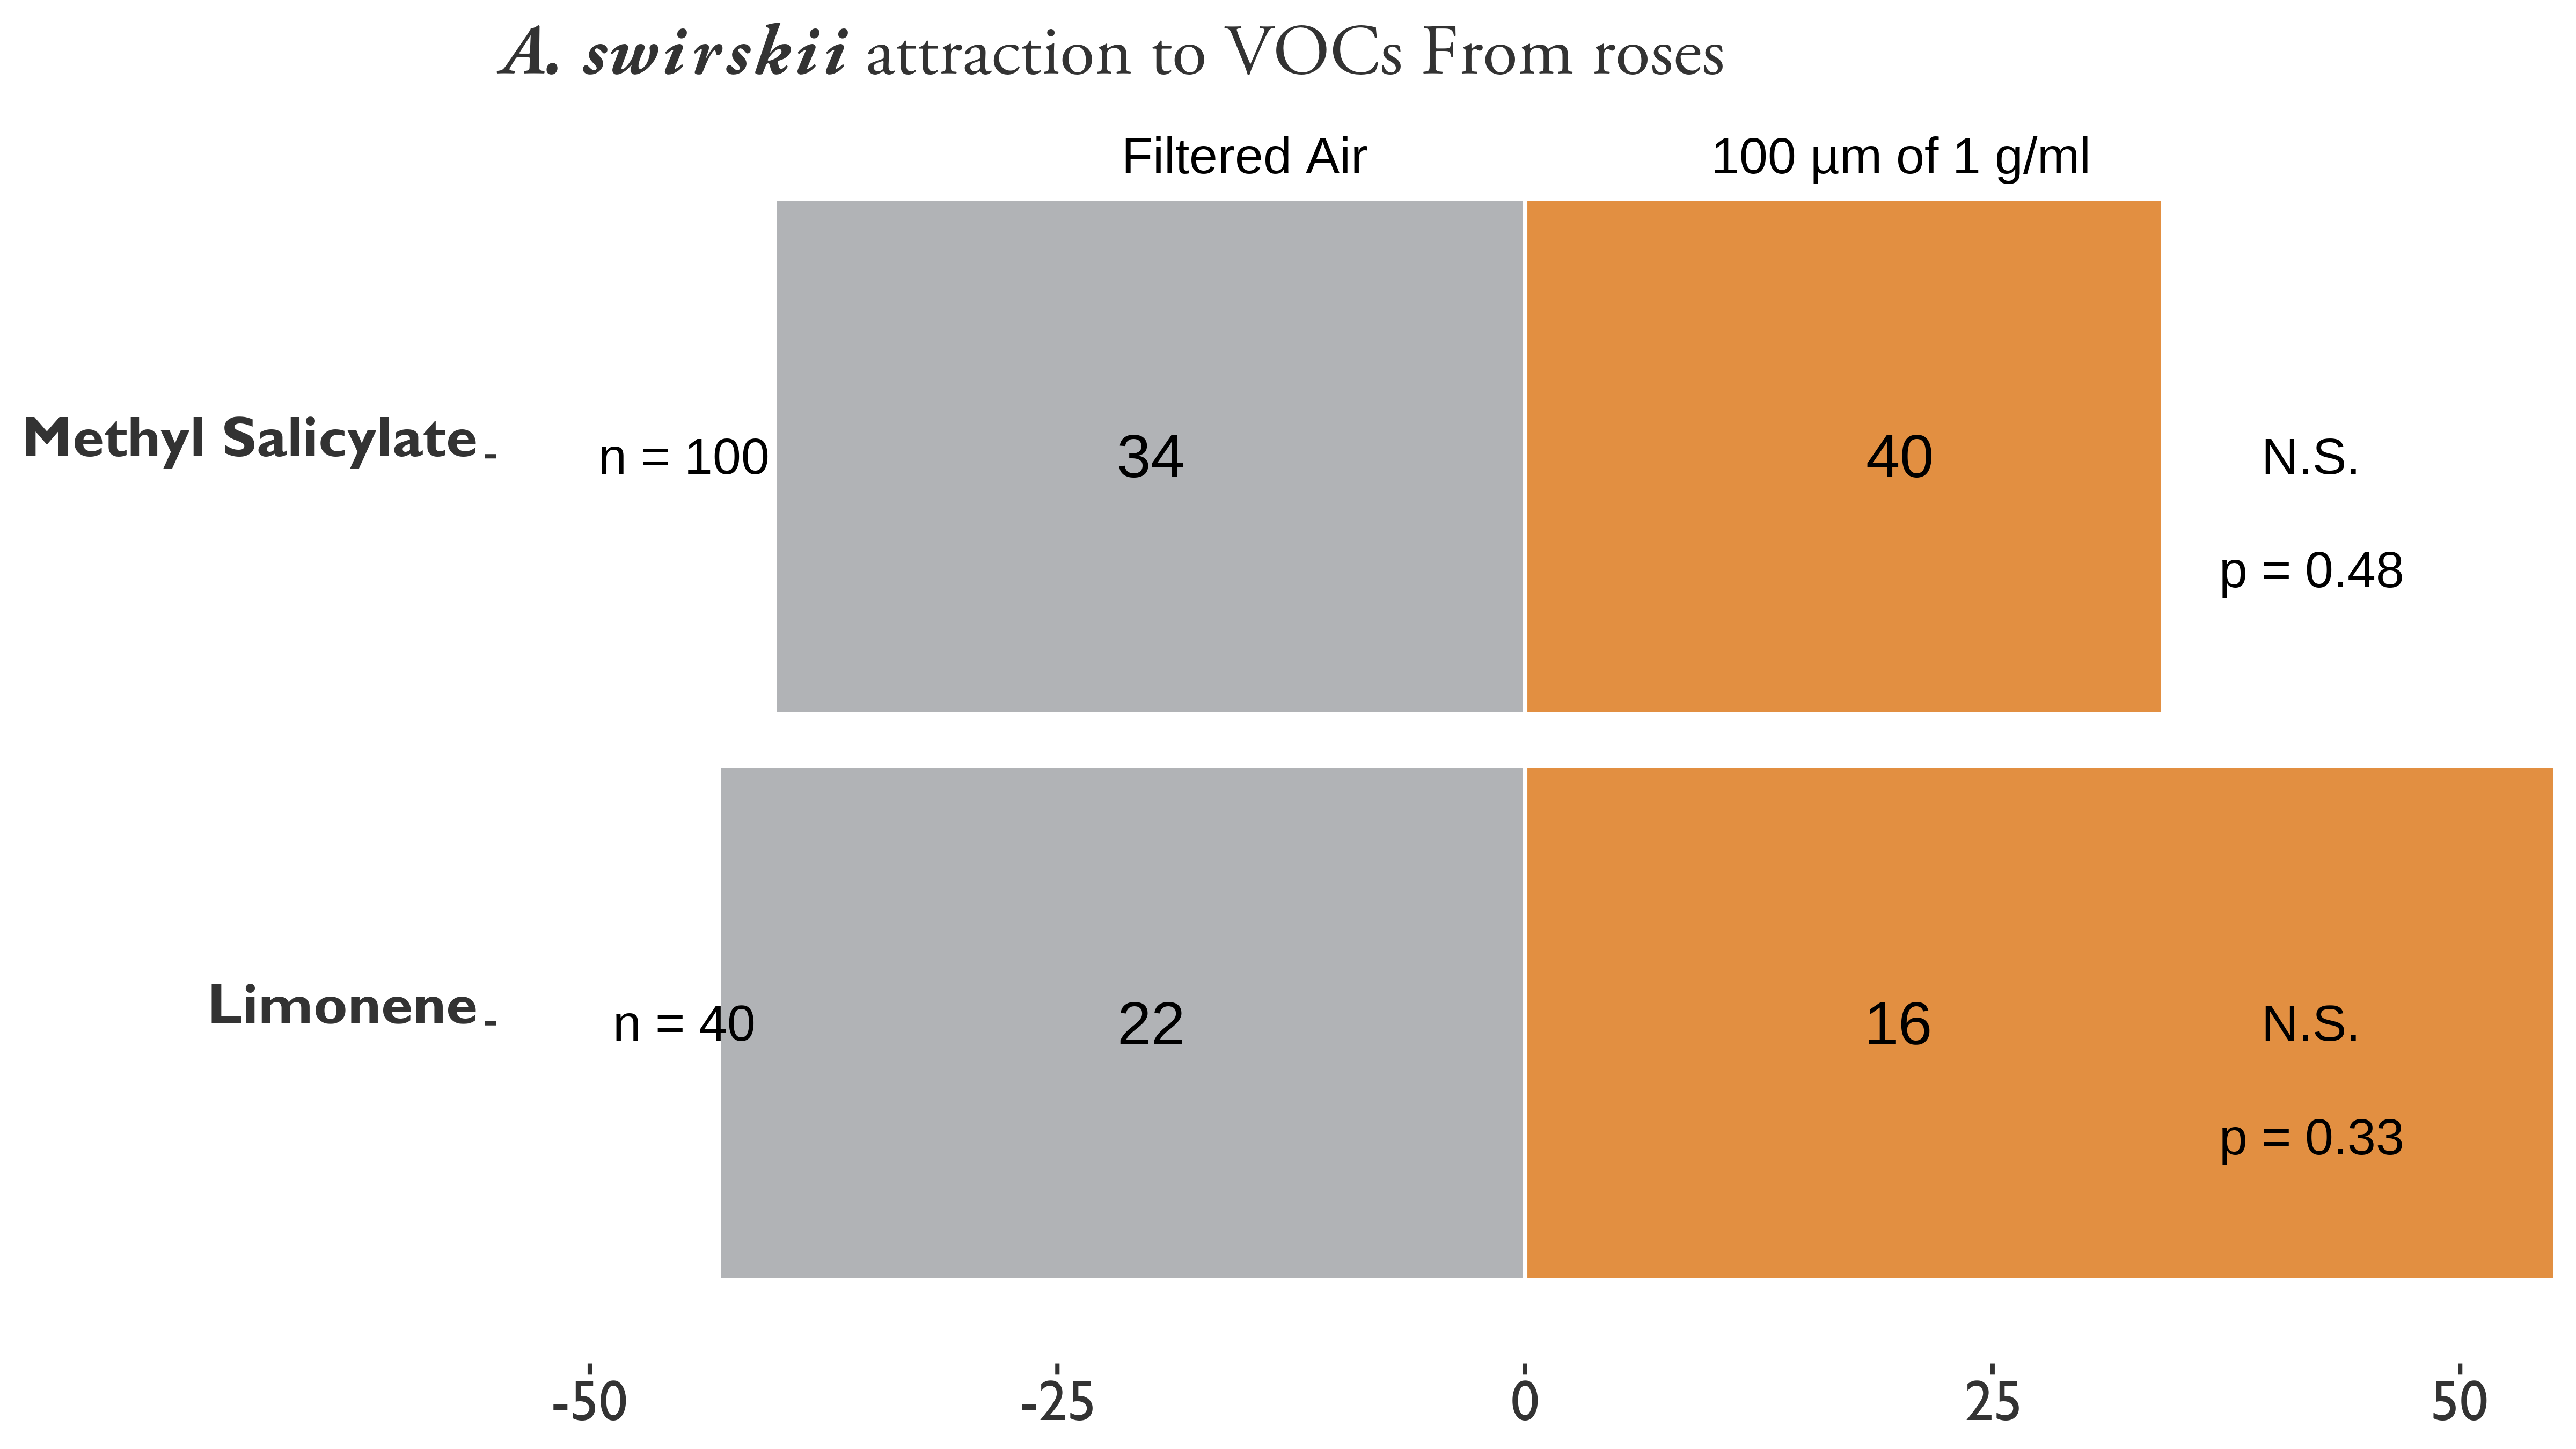
\includegraphics[width=0.8\linewidth]{figure/tests_graph} \end{center}

  Figure 12: \emph{Amblyseius swirskii} attraction to Methyl Salicylate (MeSA) and D-L Limonene vs Filtered Air at concentrations of 1 g/mL. 100 μm of chemical was applied to 3 cm dental wicks inside of erlenmeyer flasks which were part of the air line attached to the olfactometer. Asterisks represent significant differences as calculated by χ-squared contingency table tests for given probabilities. N.S. = not significant. MeSA vs Air: χ-squared = 0.48649, df = 1, a = 0.05, p-value = 0.4855. D-L Limonene vs Air: χ-squared = 0.94737, df = 1, a = 0.05, p-value = 0.3304.

  Volatiles from 20 roses will be collected before treatments as a baseline (already collected). Then half of the plants will be SAR-induced by bi-weekly spray applications of Acibenzolar-S-Methyl. Subsequently, half of the remaining plants (5 control and 5 SAR-induced plants) will be grafted with RRV-infected buds to innoculate them with the virus (Doudrick et al. 1987). Volatiles will be collected bi-monthly following SAR-induction and RRV application.
  \begin{center}\includegraphics[width=0.8\linewidth]{thesis_files/figure-latex/voc-trap-1} \end{center}

  Figure 12: \emph{Amblyseius swirskii} attraction to Methyl Salicylate (MeSA) and D-L Limonene vs Filtered Air at concentrations of 1 g/mL. 100 μm of chemical was applied to 3 cm dental wicks inside of erlenmeyer flasks which were part of the air line attached to the olfactometer. Asterisks represent significant differences as calculated by χ-squared contingency table tests for given probabilities. N.S. = not significant. MeSA vs Air: χ-squared = 0.48649, df = 1, a = 0.05, p-value = 0.4855. D-L Limonene vs Air: χ-squared = 0.94737, df = 1, a = 0.05, p-value = 0.3304.

  Expected Results:

  There will be differences in Methyl Salicylate between each group of roses: SAR-induced plants will have the most, RRV-infected roses will have the least, indicating changes in plant chemistry during RRV-infection. Other chemicals, particularly those associated with plant defenses, follow similar trends, and vary from group to group, but we have little preliminary data on this. By determining which chemicals change during infection or with SAR-induction, we can gain insight into the physiological changes occuring during RRV-infection and SAR-induction in roses. Testing headspace volatiles can also give us insight into what VOCs predators like \emph{A. swirskii} may encounter on infected or SAR-induced roses.
  \begin{itemize}
  \item
    Determine which headspace VOCs are different between RRV-infected and healthy roses
  \item
    Determine what effects SAR-induction has on RRV-infected and healthy roses
  \item
    Creates a starting point for volatile testing for future olfactometer studies with \emph{A. swirskii} and predatory mites
  \item
    Knowing which VOCs affect the host-seeking abilities of a predatory mite like \emph{A. swirskii} is part of preliminary work for determining the compatibility of predatory mites for control of \emph{P. fructiphilus}.
  \end{itemize}
  \hypertarget{expected-outcomes-2}{%
  \subsubsection{3.3.4 Expected outcomes}\label{expected-outcomes-2}}

  Potential outcomes of observing predatory mite behaviors are:
  \begin{itemize}
  \item
    Identify which RRV-infected rose compounds are attracting \emph{A. swirskii}
  \item
    Determine rate of \emph{A. swirskii} predation on \emph{P. fructiphilus}
  \end{itemize}
  Nursery managers are interested in alternative and less expensive management options to combat \emph{P. fructiphilus} and Rose Rosette Virus. Predatory mites have potential to fulfill this need: Mites from the family Phytoseiidae are being investigated as biocontrol agents for the management of \emph{P. fructiphilus}. Preliminary data suggest that the phytoseiid mite \emph{A. swirskii} is attracted to volatiles of Rose Rosette-infected roses. This attraction may have synergistic effects for \emph{P. fructiphilus} control. \emph{A. swirskii} This research will contribute testing the suitability of \emph{A. swirskii} as a biocontrol option for the management of \emph{P. fructiphilus}.

  \hypertarget{integrated-pest-management-of-phyllocoptes-fructiphilus}{%
  \chapter{\texorpdfstring{Integrated Pest Management of \emph{Phyllocoptes fructiphilus}}{Integrated Pest Management of Phyllocoptes fructiphilus}}\label{integrated-pest-management-of-phyllocoptes-fructiphilus}}

  \hypertarget{introduction}{%
  \subsection{Introduction}\label{introduction}}

  Integrated Pest Management (IPM) is the combination of science-informed best practices designed to keep the cost of pest control below the value of the crop damages which would occur without intervention (i.e.~economic injury level) (USDA-ARS 2018). In practice, IPM is informed by an understanding of the pest's biology and the judicious use of chemical controls, natural predators (biological controls), plant breeding, plant immune systems and physical (cultural) controls as needed to control pests as efficiently as possible.

  \emph{Phyllocoptes fructiphilus} Keifer (Trombidiformes: Eriophyidae) is a microscopic plant-feeding arachnid known as an eriophyid mite. \emph{P. fructiphilus} is host specific, only feeding on plants in the genus \emph{Rosa}, and normally cause little damage by itself. Unfortunately, \emph{P. fructiphilus} has become infamous due to Rose Rosette Virus (RRV), a pathogen which the mite transmits while feeding. RRV infection creates the following symptoms: witches' brooms/rosetting, deformed flowers, increased prickle density, elongated shoots, reddened leaves and stems, and increased die-back which ultimately kills the rose host. This disease is known as Rose Rosette Disease (RRD) and is widely considered the most serious disease of roses in the US. RRD and the mite have invaded the southeastern US as they followed the range expansion of the non-native \emph{Rosa multiflora} (Thunb) towards the coast (Amrine Jr 2002, Otero-Colina et al. 2018). RRD afflicts a passionate group from different sections of the US rose industry, including homeowners, commercial landscapers, nurseries, conservationists, and rosarians, all of whom stand to lose millions of dollars and many established roses plantings in the coming years. Florida, as the nation's largest producer of roses, has a special interest developing methods to better control \emph{P. fructiphilus} and RRD.

  There is a critical need to improve management of \emph{P. fructiphilus} and RRD. Unfortunately, few commercially available roses have resistance to RRD (Di Bello et al. 2017, Byrne et al. 2018). Presently, growers are recommended to manage the \emph{P. fructiphilus} by removing plants and spraying pesticides (Hong et al. 2012, Olson et al. 2017, {``Control - rose rosette''} 2018). However, pesticides have come under increased public scrutiny due to concerns about health, the environment, pest resistance, and harm to pollinators Vanbergen and Insect Pollinators Initiative (2013). Increased pesticide applications also decrease grower profits and reduce competitiveness with foreign markets. The lack of alternative or complementary management options exacerbates this issue: rose growers need more options for \emph{P. fructiphilus} control, especially methods which can be integrated into existing management programs.

  In 2013, nursery workers in Quincy, Gadsden County, Florida, USA, detected unusual red growths, deformed stems and extra thorniness on 15 knockout roses which had been imported from out of state. Eight symptomatic plants were tested by our Plant Diagnostic Clinic at the University of Florida's North Florida Research and Education Center in Quincy, FL, and found to be positive for RRD, but the \emph{P. fructiphilus} mites were not detected at that time (Babu et al. 2014).

  Since then, nurseries, rosarians, landscapers and shareholders have expressed concerns about the possible introduction of RRD infestations from areas where the disease had become established, including the neighboring states of Georgia and Alabama (Solo et al. 2020).

  Our experiments focus on a major obstacle to controlling RRD: Eriophyid mites like \emph{P. fructiphilus} are hard to control via conventional methods (i.e.~pesticides) due to their small size and their cryptic habits. \emph{P. fructiphilus} hide in tight spaces such as rose sepals and petioles, and under glandular plant hairs (Otero-Colina et al. 2018, Bauchan et al. 2019). This means that management which relies on contact with the pest is unlikely to reach these mites under normal circumstances.

  Our lab hypothesizes that predatory mites can circumvent this problem and combat \emph{P. fructiphilus} in situ. Predatory mites in the family Phytoseiidae can manage a variety of agricultural pests (Gerson et al. 2003, Carrillo et al. 2015), and some species are small enough that they may be able to find and feed on \emph{P. fructiphilus} in their hiding places (Carillo, personal communication).

  In 2017, some researchers suggested a southern limit for RRD and \emph{P. fructiphilus}, based on a series of surveys they had conducted in the Eastern US (Solo et al. 2020). The suggested boundary was thought to be caused by some unknown environmental factor(s), such as climate, pathogens, lack of a suitable host, or natural enemies in the landscape, which limited the range of RRD and \emph{P. fructiphilus}. Unfortunately, these surveys had not included Florida, possibly due to constraints on time and/or resources.

  As part of the efforts to develop novel mite management methods, our lab has leveraged its experience with chemical ecology to conduct a series of preliminary two-choice maze (Y-tube olfactometer) trials with various species of commercially-available predatory mites. In these trials, mites are exposed to chemical odorants which are correlated with the pest arthropod, such as samples droppings or sheds of the pest, a substrate which the pest has walked on, eggs of the pest, or plants which have been attacked by the pest. Attraction to these odorants is usually suggestive of predatory mite feeding preferences, and is a fast way to judge their potential for use in biological control (Janssen et al. 1990).

  While testing the compatibility of our rose system with various commercially-available predatory mites, we were excited to observe that \emph{Amblyseius swirskii} Athias-Henriot (Mesostigmata: Phytoseiidae) mites were attracted towards roses which were infected with RRD (see \emph{Figure 11}). This was encouraging because \emph{A. swirskii} are generalist predators which feed on other common agricultural pests such as whiteflies (Bolckmans et al. 2005), spider mites (McMurtry et al. 1970), and thrips (Wimmer et al. 2008), so there is good cause to believe that these mites could feed on eriophyid mites. \emph{A. swirskii} can also persist on pollen (Loughner et al. 2011, Delisle et al. 2015) and other arthropods even when the pest of concern is absent (Janssen and Sabelis 2015). This allows \emph{A. swirskii} to be released as a preventative measure instead of reacting to an outbreak (Kutuk and Yigit 2011). Furthermore, phytoseiid mites integrate well into pest management programs and are compatible with certain pesticides (Trumble and Morse 1993, Nicetic et al. 2001, Fernández et al. 2017) and other bio-control agents (Midthassel et al. 2016). Lastly, predatory mites are able to locate their prey in tight areas when other predators might be too big. These features make \emph{A. swirskii} an interesting option for managing \emph{P. fructiphilus}, where conventional methods are undesireable or unavailable.
  \begin{center}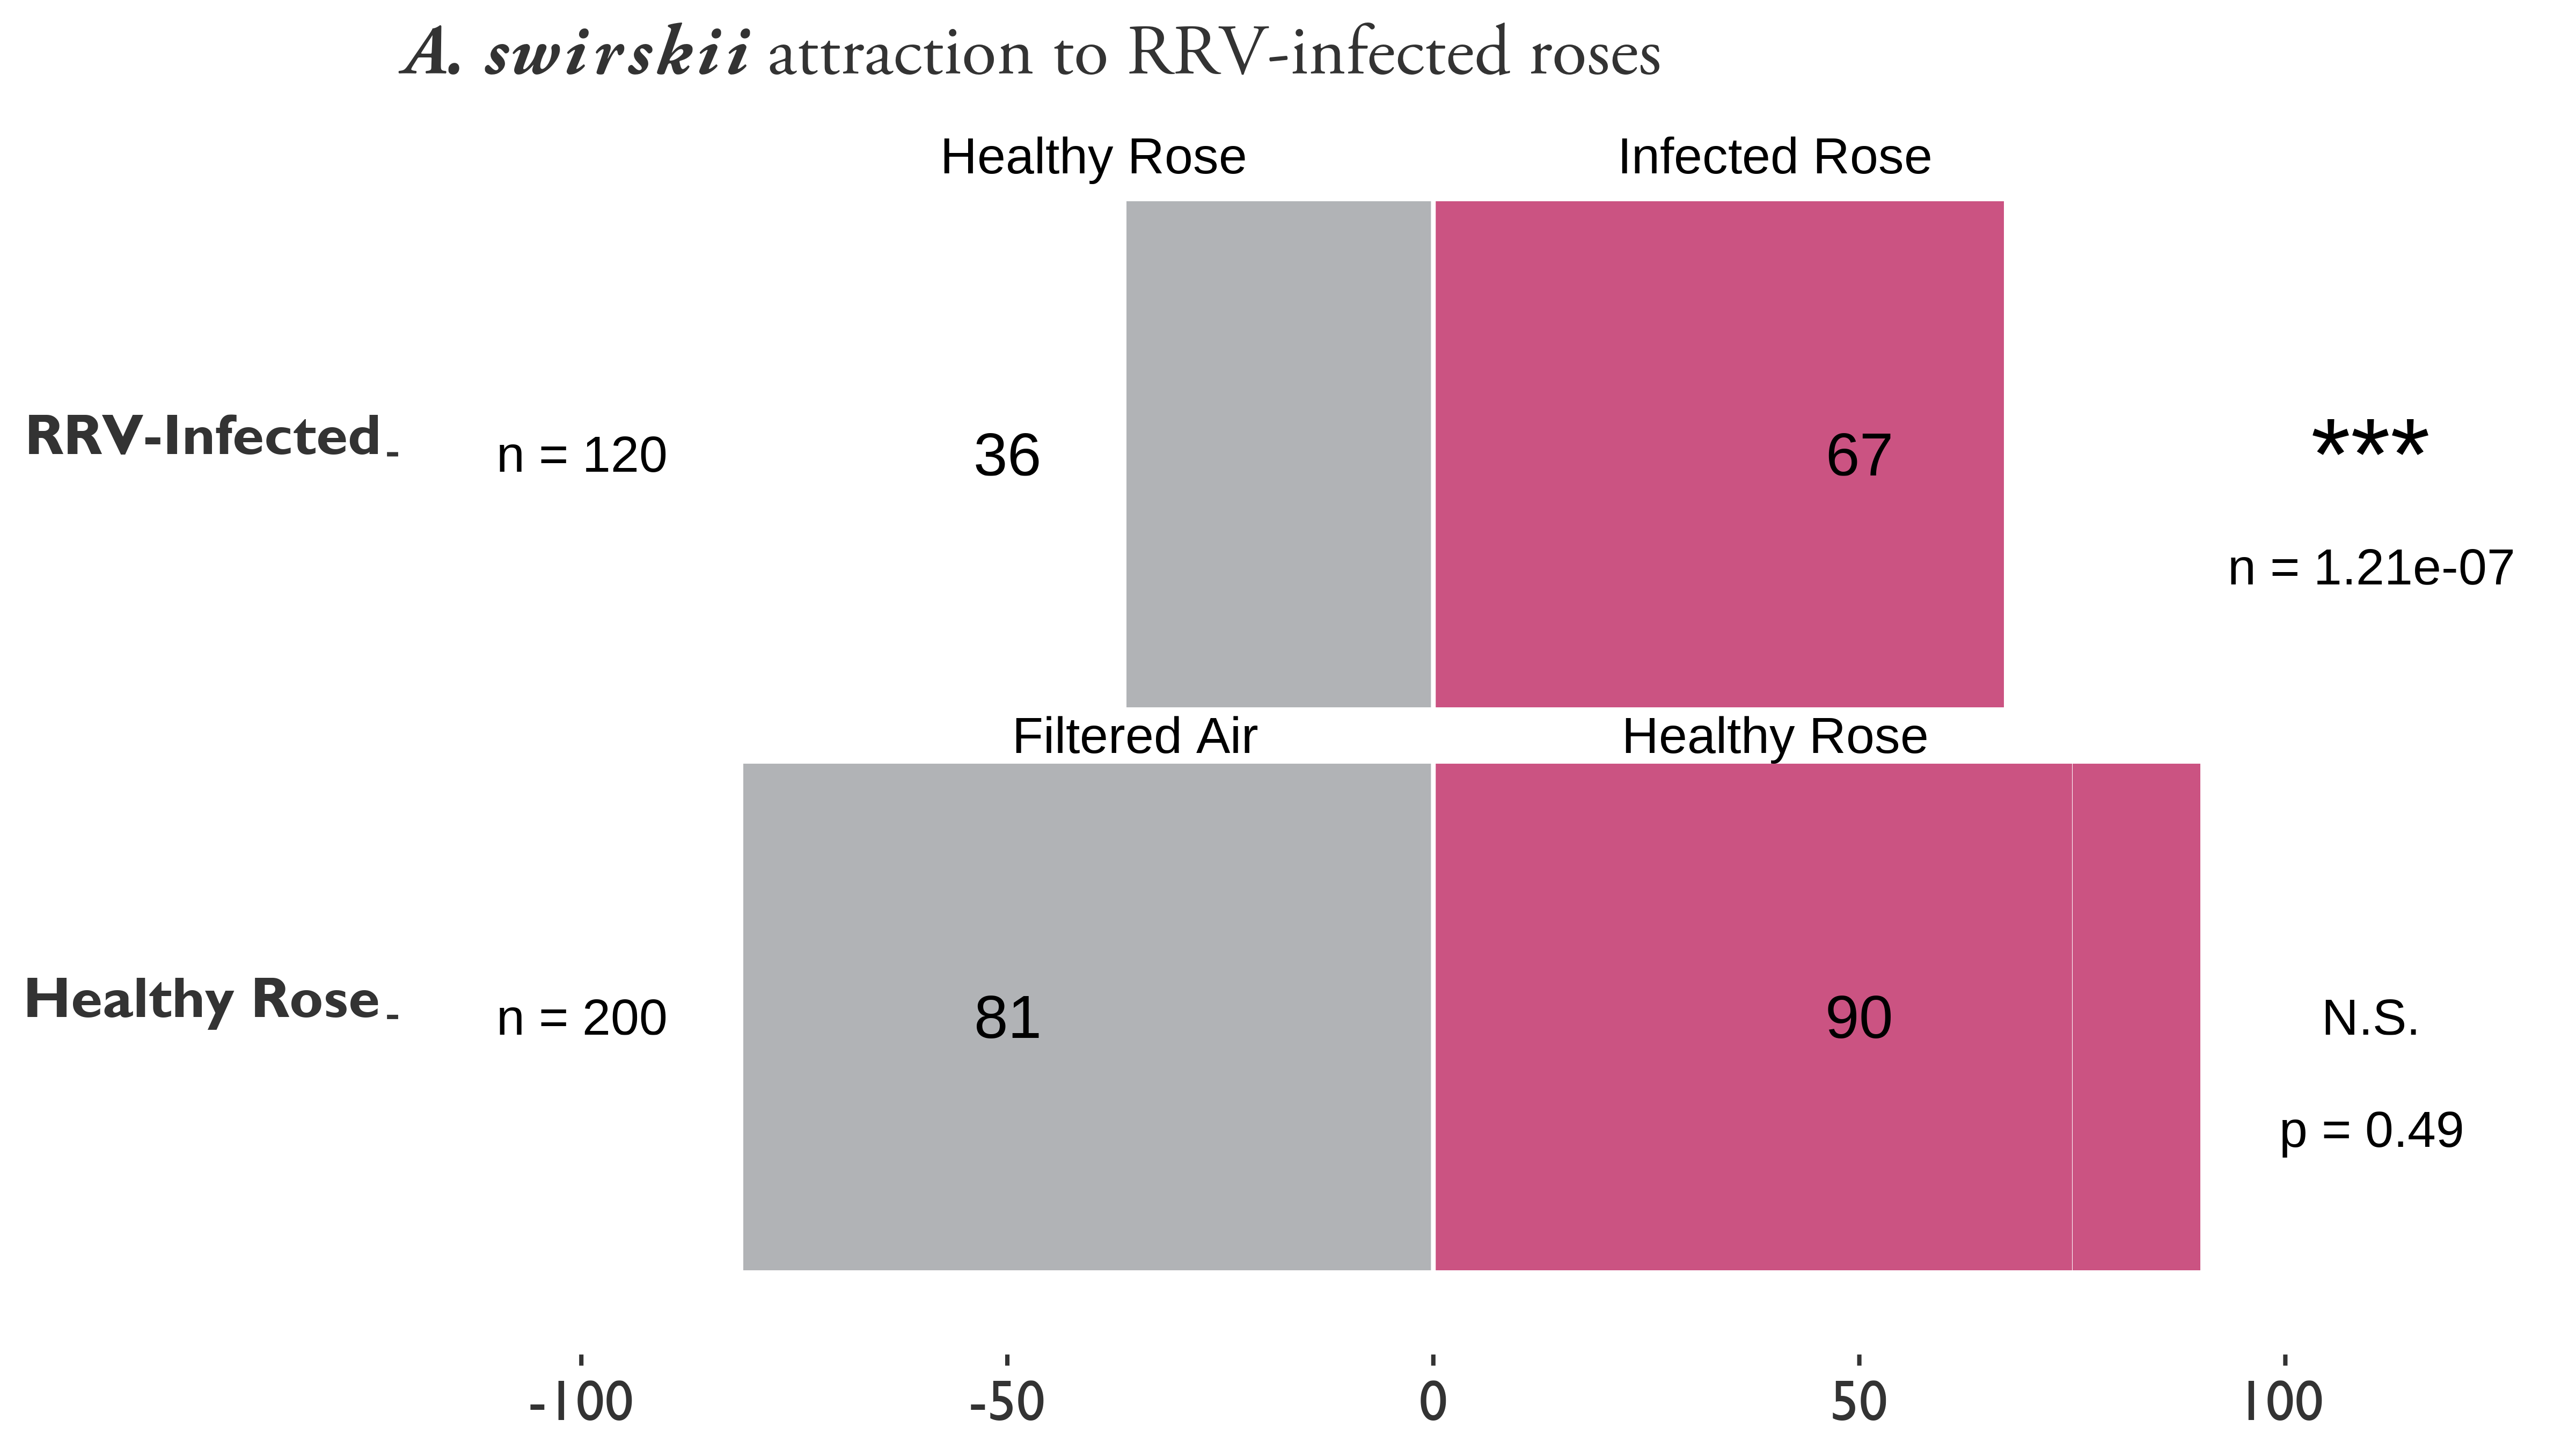
\includegraphics[width=0.8\linewidth]{figure/rose_graph} \end{center}

  Figure 11: \emph{Amblyseius swirskii} attraction to healthy and Rose Rosette Virus-infected Pink Double Knock Out® roses. Asterisks represent significant differences as calculated by χ-squared contingency table tests for given probabilities. N.S. = not significant. RRV-infected vs Healthy Rose: χ-squared = 9.33, df = 1, a = 0.05, p-value = 0.002. Filtered Air vs Healthy Rose: χ-squared = 0.47, df = 1, a = 0.05, p-value = 0.4913.

  These results compelled us to further investigate the differences between the chemical odorants (headspace volatiles) released from RRV-infected and uninfected roses using coupled Gas Chromatography-Mass Spectroscopy analysis (GC-MS). The GC-MS data revealed that RRV-infected roses had low levels of an important plant hormone known as Methyl Salicylate (MeSA). MeSA typically increases during an immune response, such as when a plant is attacked by herbivores or pathogens (Shulaev et al. 1997, Boer and Dicke 2004a). We expected high levels of MeSA in these infected roses, because they were in the middle of experiencing a pathogen attack, but contrary to this expectation, we found low levels of MeSA emitted from the RRV-infected roses. MeSA is also known to be an attractive odor to some many predatory mites, which use MeSA to locate their prey Boer and Dicke (2004a), and are often attracted to the Volatile Organic Compounds (VOCs) released when plants are injured by pests or infected with pathogens (Boer and Dicke 2004b). Our results suggest that either \emph{A. swirski} are attracted to very low levels of MeSA, or perhaps this attraction is caused by other plant chemical cues besides MeSA. Either way, identification of these VOCs gives us insight into how RRD influences the prey-seeking behaviors of \emph{A. swirksii}, which has implications for how effective predatory mite biocontrol will be.

  The most interesting part about discovering these low levels of Methyl Salicylate is the role which MeSA typically plays in pathogen resistance Park et al. (2007). MeSA is derived from the phytohormone Salicylic Acid (Tieman et al. 2010), a chemical involved when inducing a plant's immune response, known as Systemic Acquired Resistance (SAR) (Gaffney et al. 1993, Gozzo and Faoro 2013). SAR protects plants from fungi, bacteria and viral pathogens when induced and affects all tissues in the plant Ryals et al. (1994). Low levels of MeSA suggest that RRV interferes with the rose's ability to defend itself against the pathogen. A possible way to avoid this negative feedback loop is to use Salicylic Acid to induce SAR \emph{before} RRV infection, a procedure which would increase the rose's resistance to pathogens before exposure Kalaivani et al. (2016).

  In light of this knowledge, we collaborated with the University of Georgia in to test how SAR-induction might protect roses from \emph{P. fructiphilus} and/or RRD. Acibenzolar-S-methyl (ASM) is a SAR-inducing chemical which works like Salicylic Acid to induce plant defenses against viruses and bacteria Ziadi et al. (2001). ASM application also has shown chitinase activity in roses (Suo and Leung 2001), which may interfere with feeding by herbivorous mites. We tested its efficacy against mites in field trials conducted at Griffin and Athens, GA, sites with low and high \emph{P. fructiphilus} pest pressure, respectively. We tested ASM alongside a different a SAR-inducer (SP2700, Trade name `Ninja,' SePro) and combined one of the SAR-inducers with predatory mites to observe any synergistic effects. We used a miticide as a negative control and water as a positive control. (see \emph{Figure 14}). Combining predatory mites with a SAR-inducer was as effective as the miticide alone, and controlled herbivorous mite populations more than either SAR-induction or predatory mites alone (see \emph{Figure 14}).
  \begin{center}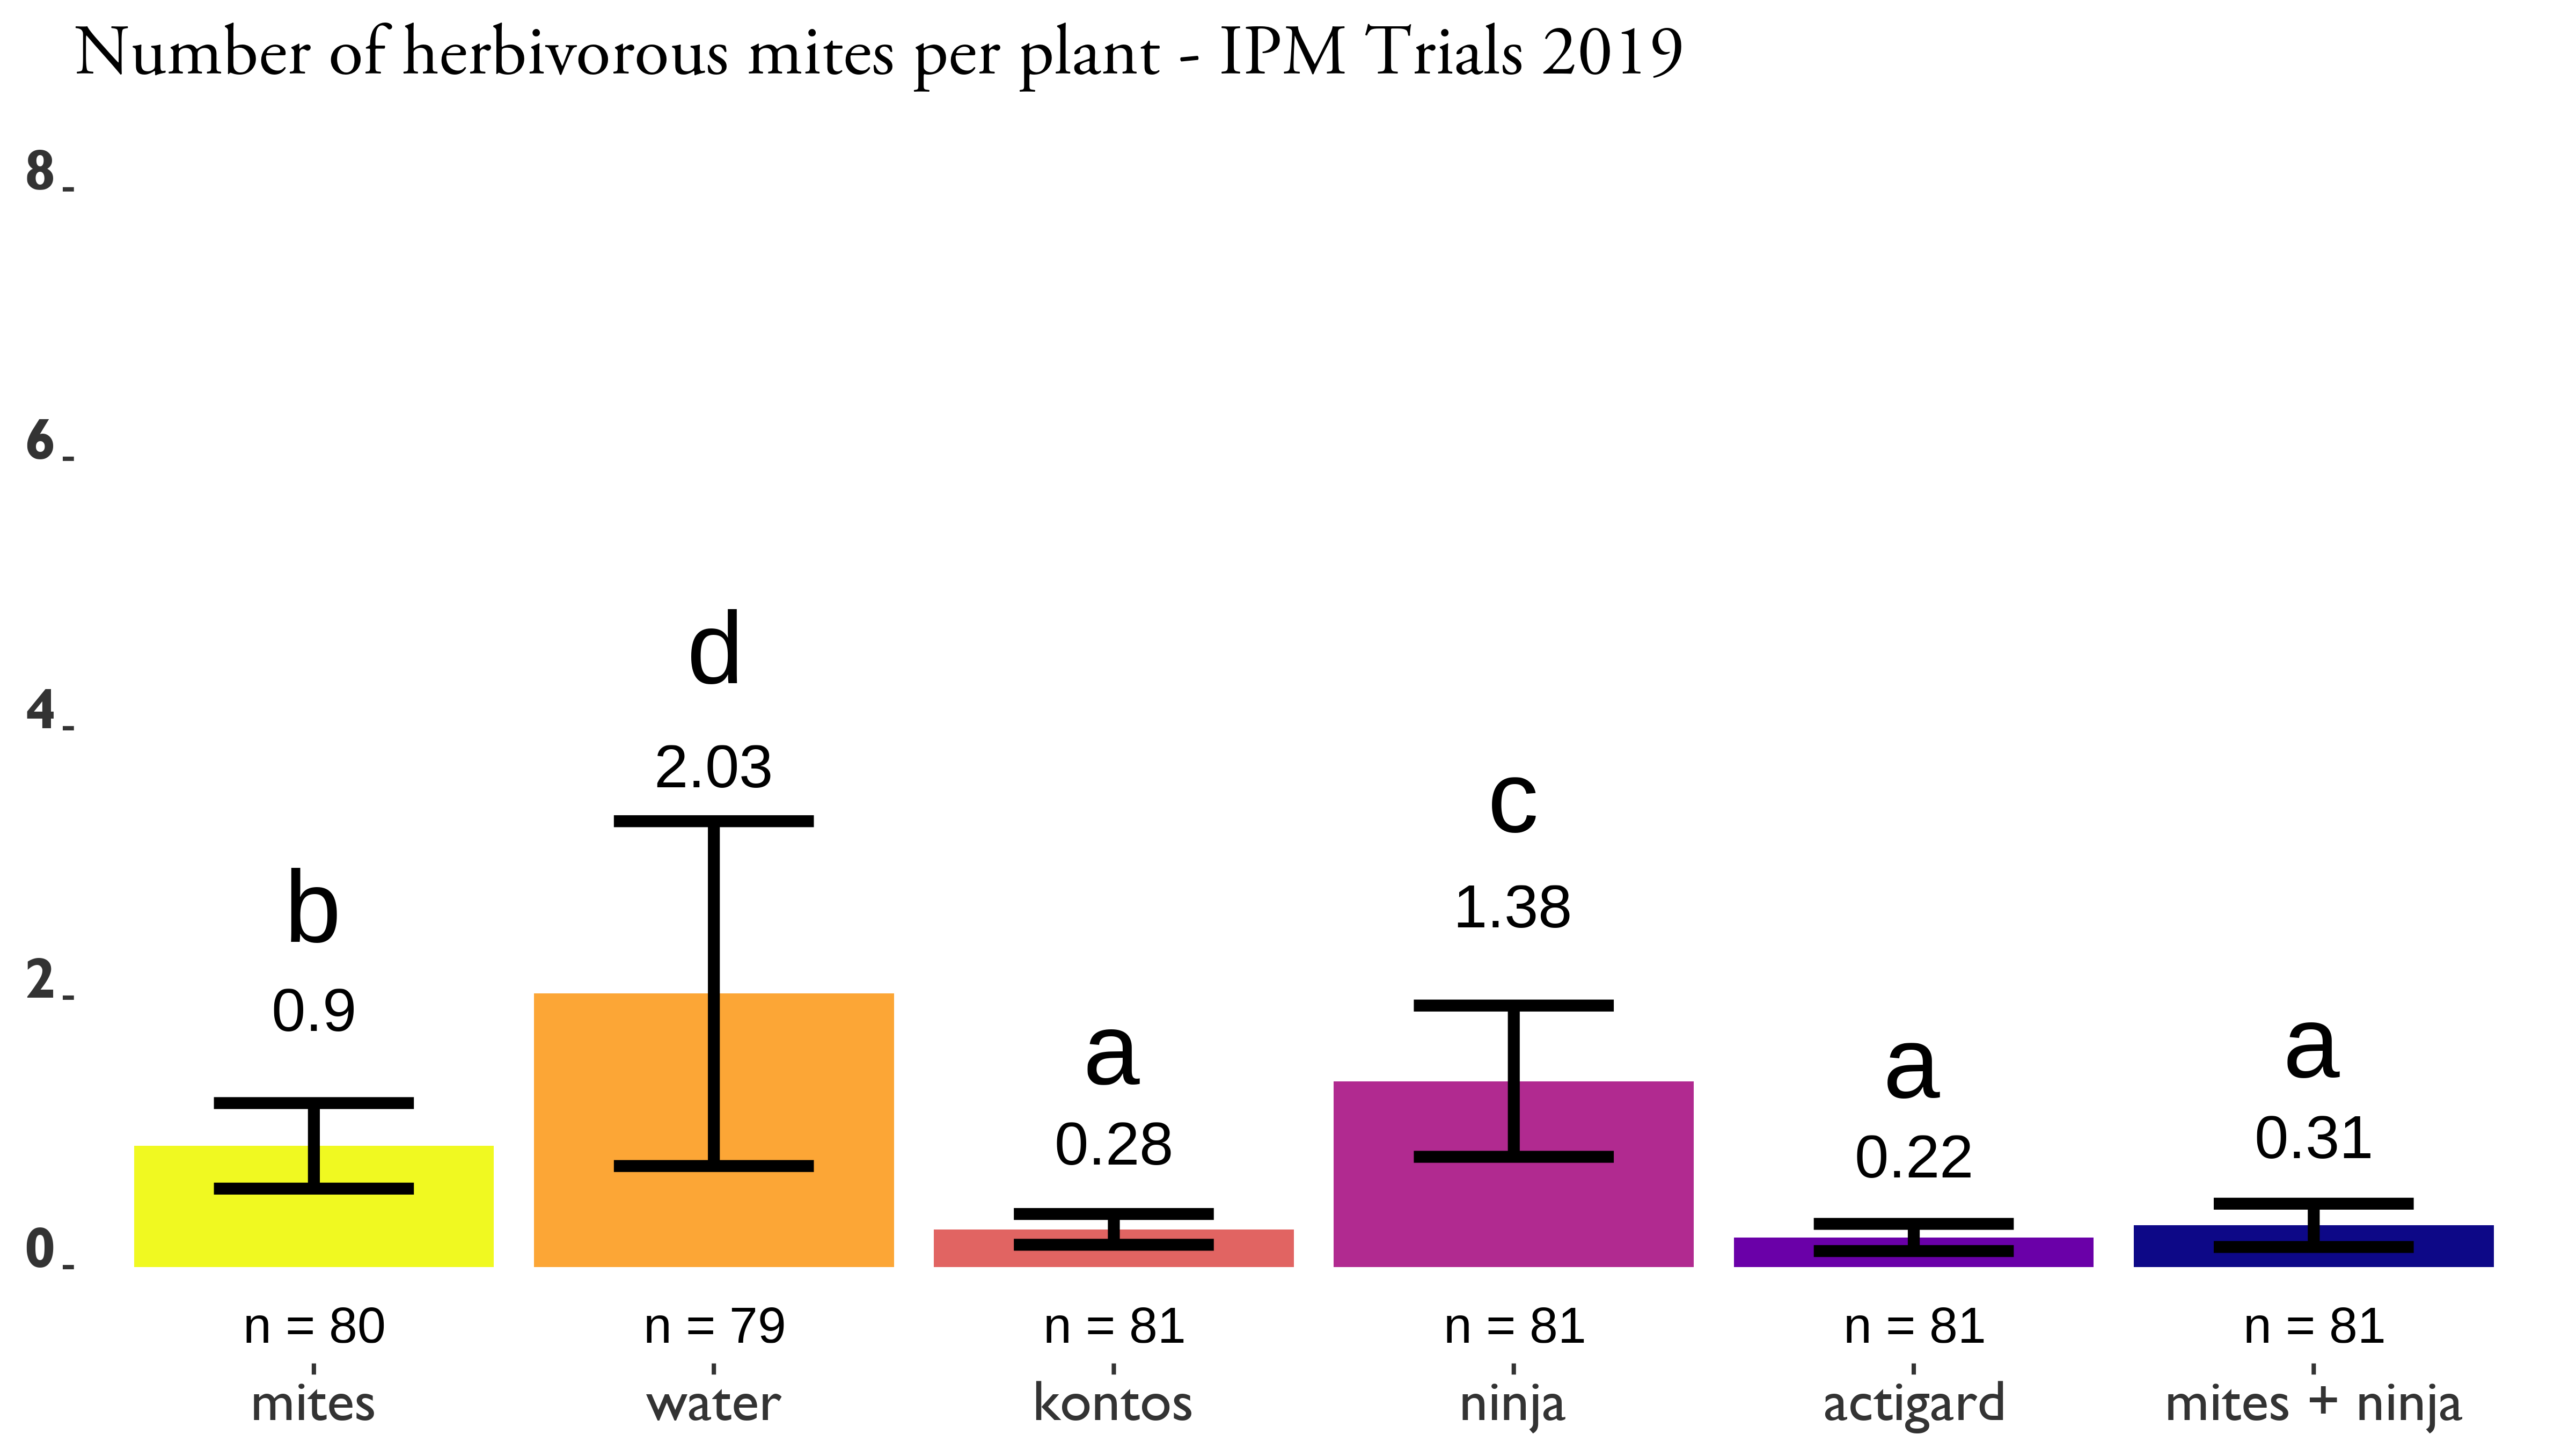
\includegraphics[width=0.8\linewidth]{figure/ipm_graph} \end{center}

  Figure 14: Integrated Pest Management trials on Pink Double Knock Out® roses to control \emph{Phyllocoptes fructiphilus} in Athens and Griffin, GA with five treatments. water = Water Control, actigard = Actigard 50WG, Acibenzolar-S-methyl (Syngenta), kontos = Kontos Miticide Insecticide (Bayer), mites = \emph{Amblyseius swirkii} predatory mite mini sachets on hooks (Arbico-organics), ninja = SP2700 (Trade name: Ninja, SePro), mites + ninja = \emph{A. swirskii} + Ninja combined treatments. All products were applied at their label rates for 12 weeks. Flower cuttings were be taken weekly to record the numbers of herbivorous mites.

  Our results suggest that SAR-induced plant defenses have the potential to manage populations of \emph{P. fructiphilus}, especially when integrating SAR-induction with predatory mites. A remaining concern is the effect that SAR-induction has on predatory mite releases: although predatory mites do not feed directly on plants, they may still be harmed via direct and indirect effects of SAR-induction Pappas et al. (2017). We assert that this less-explored area merits further research in order to optimize the integration of predatory mites with SAR.

  Rose Rosette Virus (RRV) is a lethal emaravirus (Emaraviridae) vectored by \emph{Phyllcoptes fructiphilus} Kiefer as it feeds (Allington et al. 1968, Laney et al. 2011). RRV creates a condition known as Rose Rosette Disease (RRD), with the following symptoms: witches' brooms/rosetting, deformed flowers, increased prickle density, elongated shoots, reddened leaves and stems, increased die-back and ultimately rose death.

  RRV and \emph{P. fructiphilus} are widely distributed in the US, and

  Integrated Pest Management (IPM) is the combination of science-informed best practices designed to keep the cost of pest control below the value of the crop damages which would occur without intervention (i.e.~economic injury level) (USDA-ARS 2018). In practice, IPM is informed by an understanding of the pest's biology and the judicious use of chemical controls, natural predators (biological controls), plant breeding, plant immune systems and physical (cultural) controls as needed to control pests as efficiently as possible.

  Currently, no roses are known to resist \emph{P. fructiphilus} and few roses show signs of resistance to RRV (Di Bello et al. 2017). Horticulturists manage the disease by removing sick plants and spraying pesticides in an attempt to kill the mite vector. Pesticides are under increased public scrutiny due to concerns about health, the environment, and harm to pollinators.

  Acaricide applications are expensive, and eriophyid mites may develop resistance to acaricides with increased applications (Omoto et al. 1995).

  Overall, rose growers need better methods to combat \emph{P. fructiphilus} and RRV.

  Our preliminary data have revealed quantitative and qualitative differences of headspace volatiles between RRV-infected and uninfected roses, including Methyl Salicylate (MeSA). MeSA is derived from the phytohormone Salicylic Acid (SA) (Tieman et al. 2010), a chemical involved in inducing a plant's immune response, known as Systemic Acquired Resistance (SAR) (Gaffney et al. 1993, Tieman et al. 2010, Tripathi et al. 2010, Gozzo and Faoro 2013, Kalaivani et al. 2016). MeSA typically increases during an immune response (Shulaev et al. 1997), but we found low levels emitted from infected roses. We intend to investigate if we can detect early RRV - infection by monitoring these differences in MeSA and related volatile emissions over time.

  Phytoseiid mites such as \emph{A. swirskii} are predatory mites which are commercially available and have been used successfully in agriculture for pest control (Smith and Papacek 1991, Onzo et al. 2012, Buitenhuis et al. 2015). Phytoseiid mites integrate well into pest management programs and are compatible with certain pesticides (Trumble and Morse 1993, Nicetic et al. 2001, Fernández et al. 2017) and other bio-control agents (Midthassel et al. 2016).

  \emph{A. swirskii} are generalist predators which feed on other agricultural pests such as whiteflies (Bolckmans et al. 2005), spider mites (McMurtry et al. 1970), and thrips (Wimmer et al. 2008). \emph{A. swirskii} can persist on pollen (Loughner et al. 2011, Delisle et al. 2015) or other arthropods in the field even when the pest of concern is absent (Janssen and Sabelis 2015). This allows \emph{A. swirskii} to be released before the targeted pest is present (Kutuk and Yigit 2011). Predatory mites do not feed on plants and so are not likely to be affected by ASM applications. This suggests that we may be able to combine predatory mites with our ASM applications to increased pest control. These features make \emph{A. swirskii} and similar mite species an attractive option for IPM, but their potential to control \emph{P. fructiphilus} has not yet been investigated. We intend to observe predatory mite behavior and chemical ecology with choice tests, prey consumptive rates, olfactometer assays, and field releases to determine which species provide optimal control of \emph{P. fructiphilus}.

  Another facet of IPM is the plant immune system itself. SAR can be induced before microbial attack to increase a plant's resistance to future microbial attack Kalaivani et al. (2016). Acibenzolar-S-methyl (ASM) is a functional analog of SA, which induces SAR (Ziadi et al. 2001, Tripathi et al. 2010). Preliminary studies have shown that ASM might prevent RRV progression in roses. ASM application also has shown chitinase activity in roses (Suo and Leung 2001), which may interfere with feeding by \emph{P. fructiphilus}. We intend to test how ASM affects RRV progression and \emph{P. fructiphilus} survival.

  Integrated pest management (IPM) techniques may have the potential to address some of the shortcomings of current control methods (\textbf{citation?}). All viable combinations of chemical and biological control are used in IPM to reduce pest populations to below the economic injury level of the crop in question (\textbf{citation?}). By not relying on a single product or method for pest control, IPM is thought to delay or prevent the development of pesticide resistance (\textbf{citation?}).

  A major aspect of integrated pest management in crops relies on the plant's natural defenses {[}{]}.

  innate immune system (Nurnberger et al. 2004). Plants naturally have resistance genes which protect plants against certain pathogens (Grennan 2006), as well as as suite of pathogen/microbe-associated molecular patterns (PAMPs/MAMPs) which are able to recognize parts of invasive pathogens which are not present in plants, such as flagellar proteins (Nurnberger et al. 2004). Plants respond to pathogen detection with the activation of signalling pathways (Biere and Bennett 2013, Gozzo and Faoro 2013). The type of biochemical response is multivariate, based on the pathways involved and the species of plant in question (\textbf{citation?}), but activation of an immune response ultimately results in a variety of biophysical/biochemical changes in plant physiology, such as the thickening of cell walls or production of antimicrobial agents, proteins, reactive oxygen species and other defensive compounds (Chisholm et al. 2006, Jones and Dangl 2006, Kachroo and Robin 2013).

  The most well-studied hormones known for triggering plant immunity are Jasmonic Acid, Ethylene, and Salicylic Acid (Thomma et al. 2001).

  These signalling pathways respond to particular types of pest and pathogen attacks, and many of the pathways overlap or interact with one another in both complementary and antagonistic ways.

  Activation of the Salicylic Acid pathway causes a plant defense response known as known as Systemic Acquired Resistance (SAR) (Gozzo and Faoro 2013). SAR can protect a plant from becoming infected, but SAR can also be activated before infection to increase a plant's resistance to future microbial attack Kalaivani et al. (2016). This is done by exposing plants to chemicals similar to Salicylic Acid (SA), a defensive phytohormone which initiates the signalling cascade for SAR (Gaffney et al. 1993).

  \hypertarget{ipm-actigard}{%
  \section{\texorpdfstring{Inducing Systemic Acquired Resistance with Acibenzolar-S-Methyl to reduce populations of \emph{Phyllocoptes fructiphilus}}{Inducing Systemic Acquired Resistance with Acibenzolar-S-Methyl to reduce populations of Phyllocoptes fructiphilus}}\label{ipm-actigard}}

  Acibenzolar-S-methyl (ASM) is a functional analog of SA, which is able to induce SAR(Ziadi et al. 2001, Tripathi et al. 2010). ASM is currently used by growers to protect plants from fungal infection (Ziadi et al. 2001, Tripathi et al. 2010). ASM application has shown chitinase activity in roses (Suo and Leung 2001) and preliminary studies have shown that ASM might prevent RRV progression in roses (Babu et al., submitted). Mites have an exoskeleton comprised of chitin (Nuzzaci and Alberti 1996), suggesting that rose chitinases affect \emph{P. fructiphilus}'s ability to feed or grow on SAR-induced plants. We intend to test how ASM affects RRV progression and \emph{P. fructiphilus} survival by testing two rates of an ASM-based SAR activator on mite populations in areas with high pest pressure in Georgia. Our hypothesis is that there will be fewer \emph{P. fructiphilus} on plants treated with Actigard when compared to the water treated control group.

  \hypertarget{materials-methods-3}{%
  \subsubsection{4.1.4 Materials \& Methods}\label{materials-methods-3}}

  \textbf{Roses}
  This will be a 12-week experiment conducted from August to October simultaneously in Griffin, GA and Athens, GA.
  Each site will be given 48 Pink Double Knock Out® Roses (Star Roses and Plants, West Grove, PA, USA) which will be planted in 1 gallon buckets filled with potting soil and mixed with granular slow-release fertilizer. Plants will be placed on black plastic mulch and be watered weekly with overhead impact sprinklers.

  \textbf{Mites}
  \emph{Phyllocoptes fructiphilus} are present in the landscape of Georgia. Tissue from RRD-infected roses will be placed onto roses during the first week and 5th week

  \textbf{Spray rates}
  We will be applying the Acibenzolar-S-methyl (ASM) based Actigard50WG® (Syngenta AG, Basel, Switzerland), at two different rates: 50 mg/L (Half rate) and 100 mg/L (High rate) to observe the effects of inducing Systemic Acquired Resistance (SAR) on \emph{Phyllocoptes fructiphilus} Kiefer. We will have two field sites in Georgia with local populations of \emph{P. fructiphilus}: Griffin GA and Athens, GA. The tests in Griffin will have two controls for chemical applications in this experiment: The first will be the miticide Kontos (Bayer CropScience LP, Cary, NC, USA), at the label rate as a positive control and the second will be water as a negative control. The tests in Athens will have a control of untreated roses as well as water as a negative control.

  \textbf{Data Collection}
  Rose/rosebud cuttings \textasciitilde10 cm will be taken from each plant before the first treatment to determine the initial populations of \emph{P. fructiphilus} on the roses. We will then take a subset of samples from each rose treatment weekly, rotating samples until each rose plant has been sampled three times. We will also collect samples from all roses at the end of the trial. This experiment will be repeated for two seasons. Rose samples will be placed in 50 mL centrifuge tubes and refrigerated or frozen until floral samples can be processed. Samples will be processed using the washing methods of Monfreda et al. (2007), eriophyoid mites will be counted and identified as previously described.

  \textbf{Plot Design - 2018}
  \begin{center}
\includegraphics[width=0.8\linewidth]{figure/reed} \end{center}

  Figure 15: Field design for testing the potential of Acibenzolar-S-Methyl to reduce populations of \emph{P. fructiphilus} by inducing Systemic Acquired Resistance in Pink Double Knock Out® roses. Trials were conducted for three months from August to October 2018 in Griffin, GA. Four treatments were applied weekly for 12 weeks: Blue = Water Red = Actigard50WG 100 mg/L (High rate), Pink = Actigard50WG 100 mg/L (Half rate) Turquoise = Kontos (Label rate). Flower cuttings were be taken weekly to record \emph{P. fructiphilus} numbers.

  \textbf{Plot Design - 2018}
  \begin{center}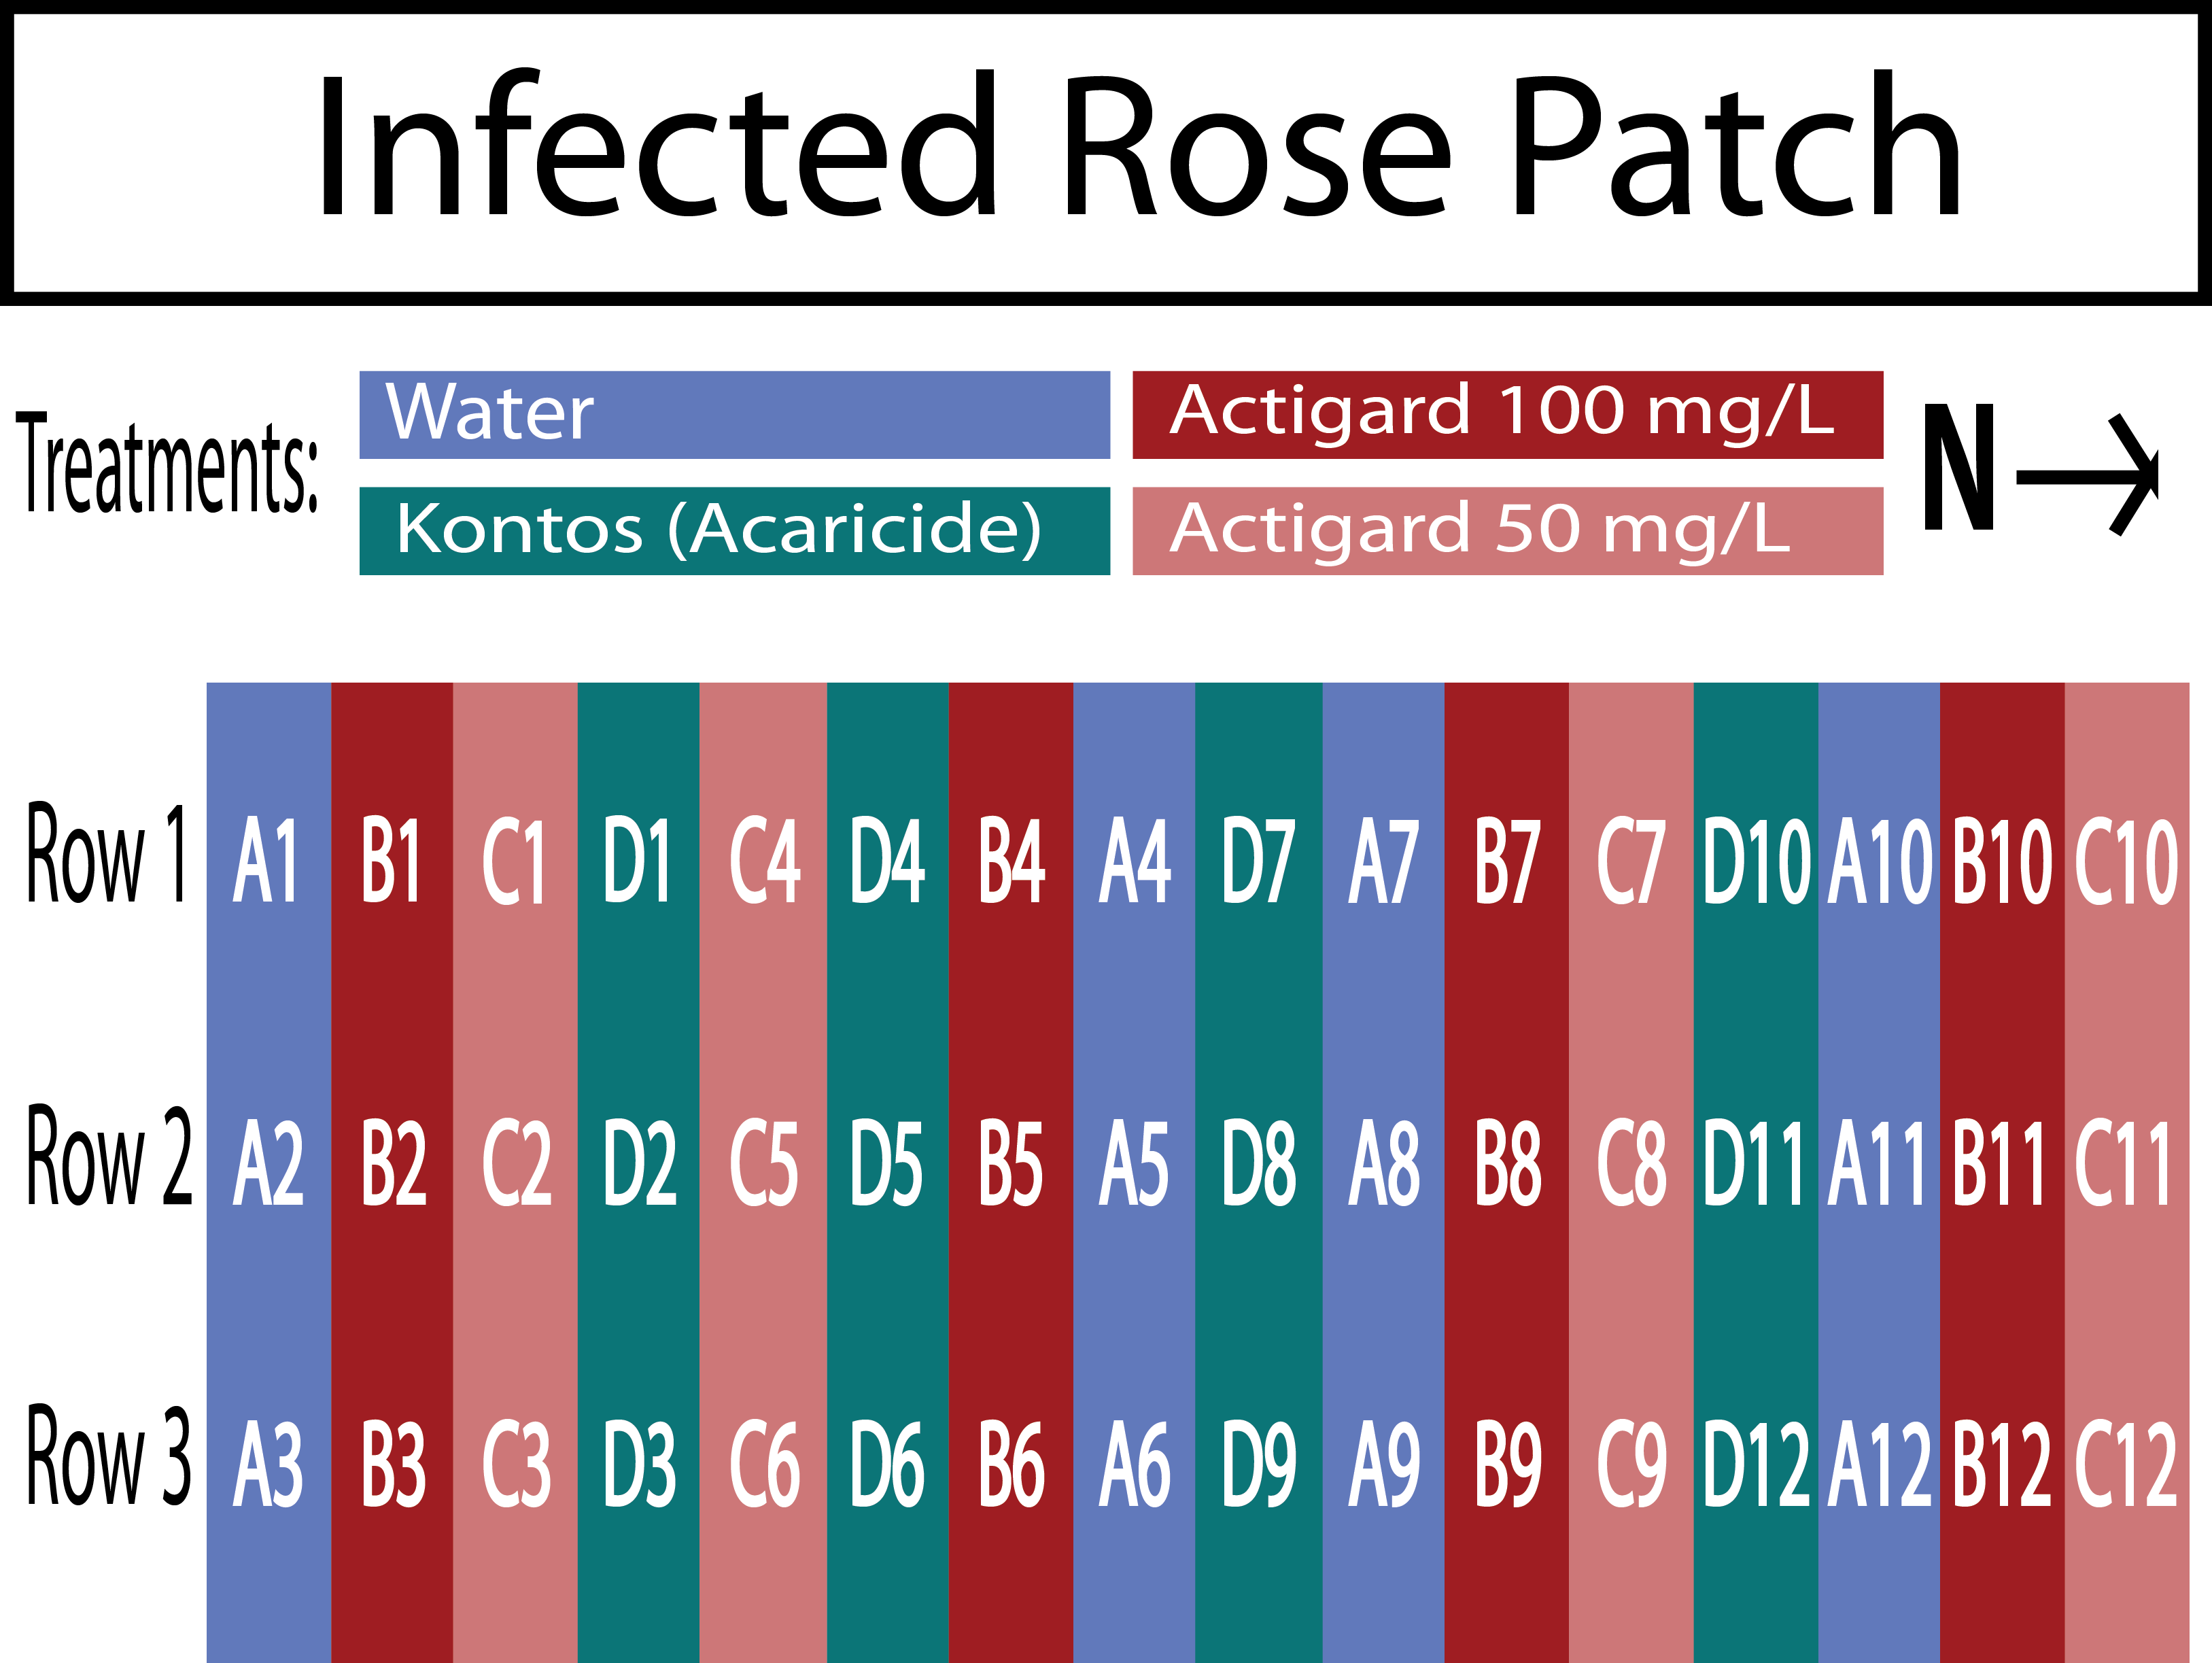
\includegraphics[width=0.8\linewidth]{figure/rrv_asm_plot_2018_griffin} \end{center}

  Figure 15: Field design for testing the potential of Acibenzolar-S-Methyl to reduce populations of \emph{P. fructiphilus} by inducing Systemic Acquired Resistance in Pink Double Knock Out® roses. Trials were conducted for three months from August to October 2018 in Griffin, GA. Four treatments were applied weekly for 12 weeks: Blue = Water Red = Actigard50WG 100 mg/L (High rate), Pink = Actigard50WG 100 mg/L (Half rate) Turquoise = Kontos (Label rate). Flower cuttings were be taken weekly to record \emph{P. fructiphilus} numbers.

  \textbf{Plot Design - 2019}
  \begin{center}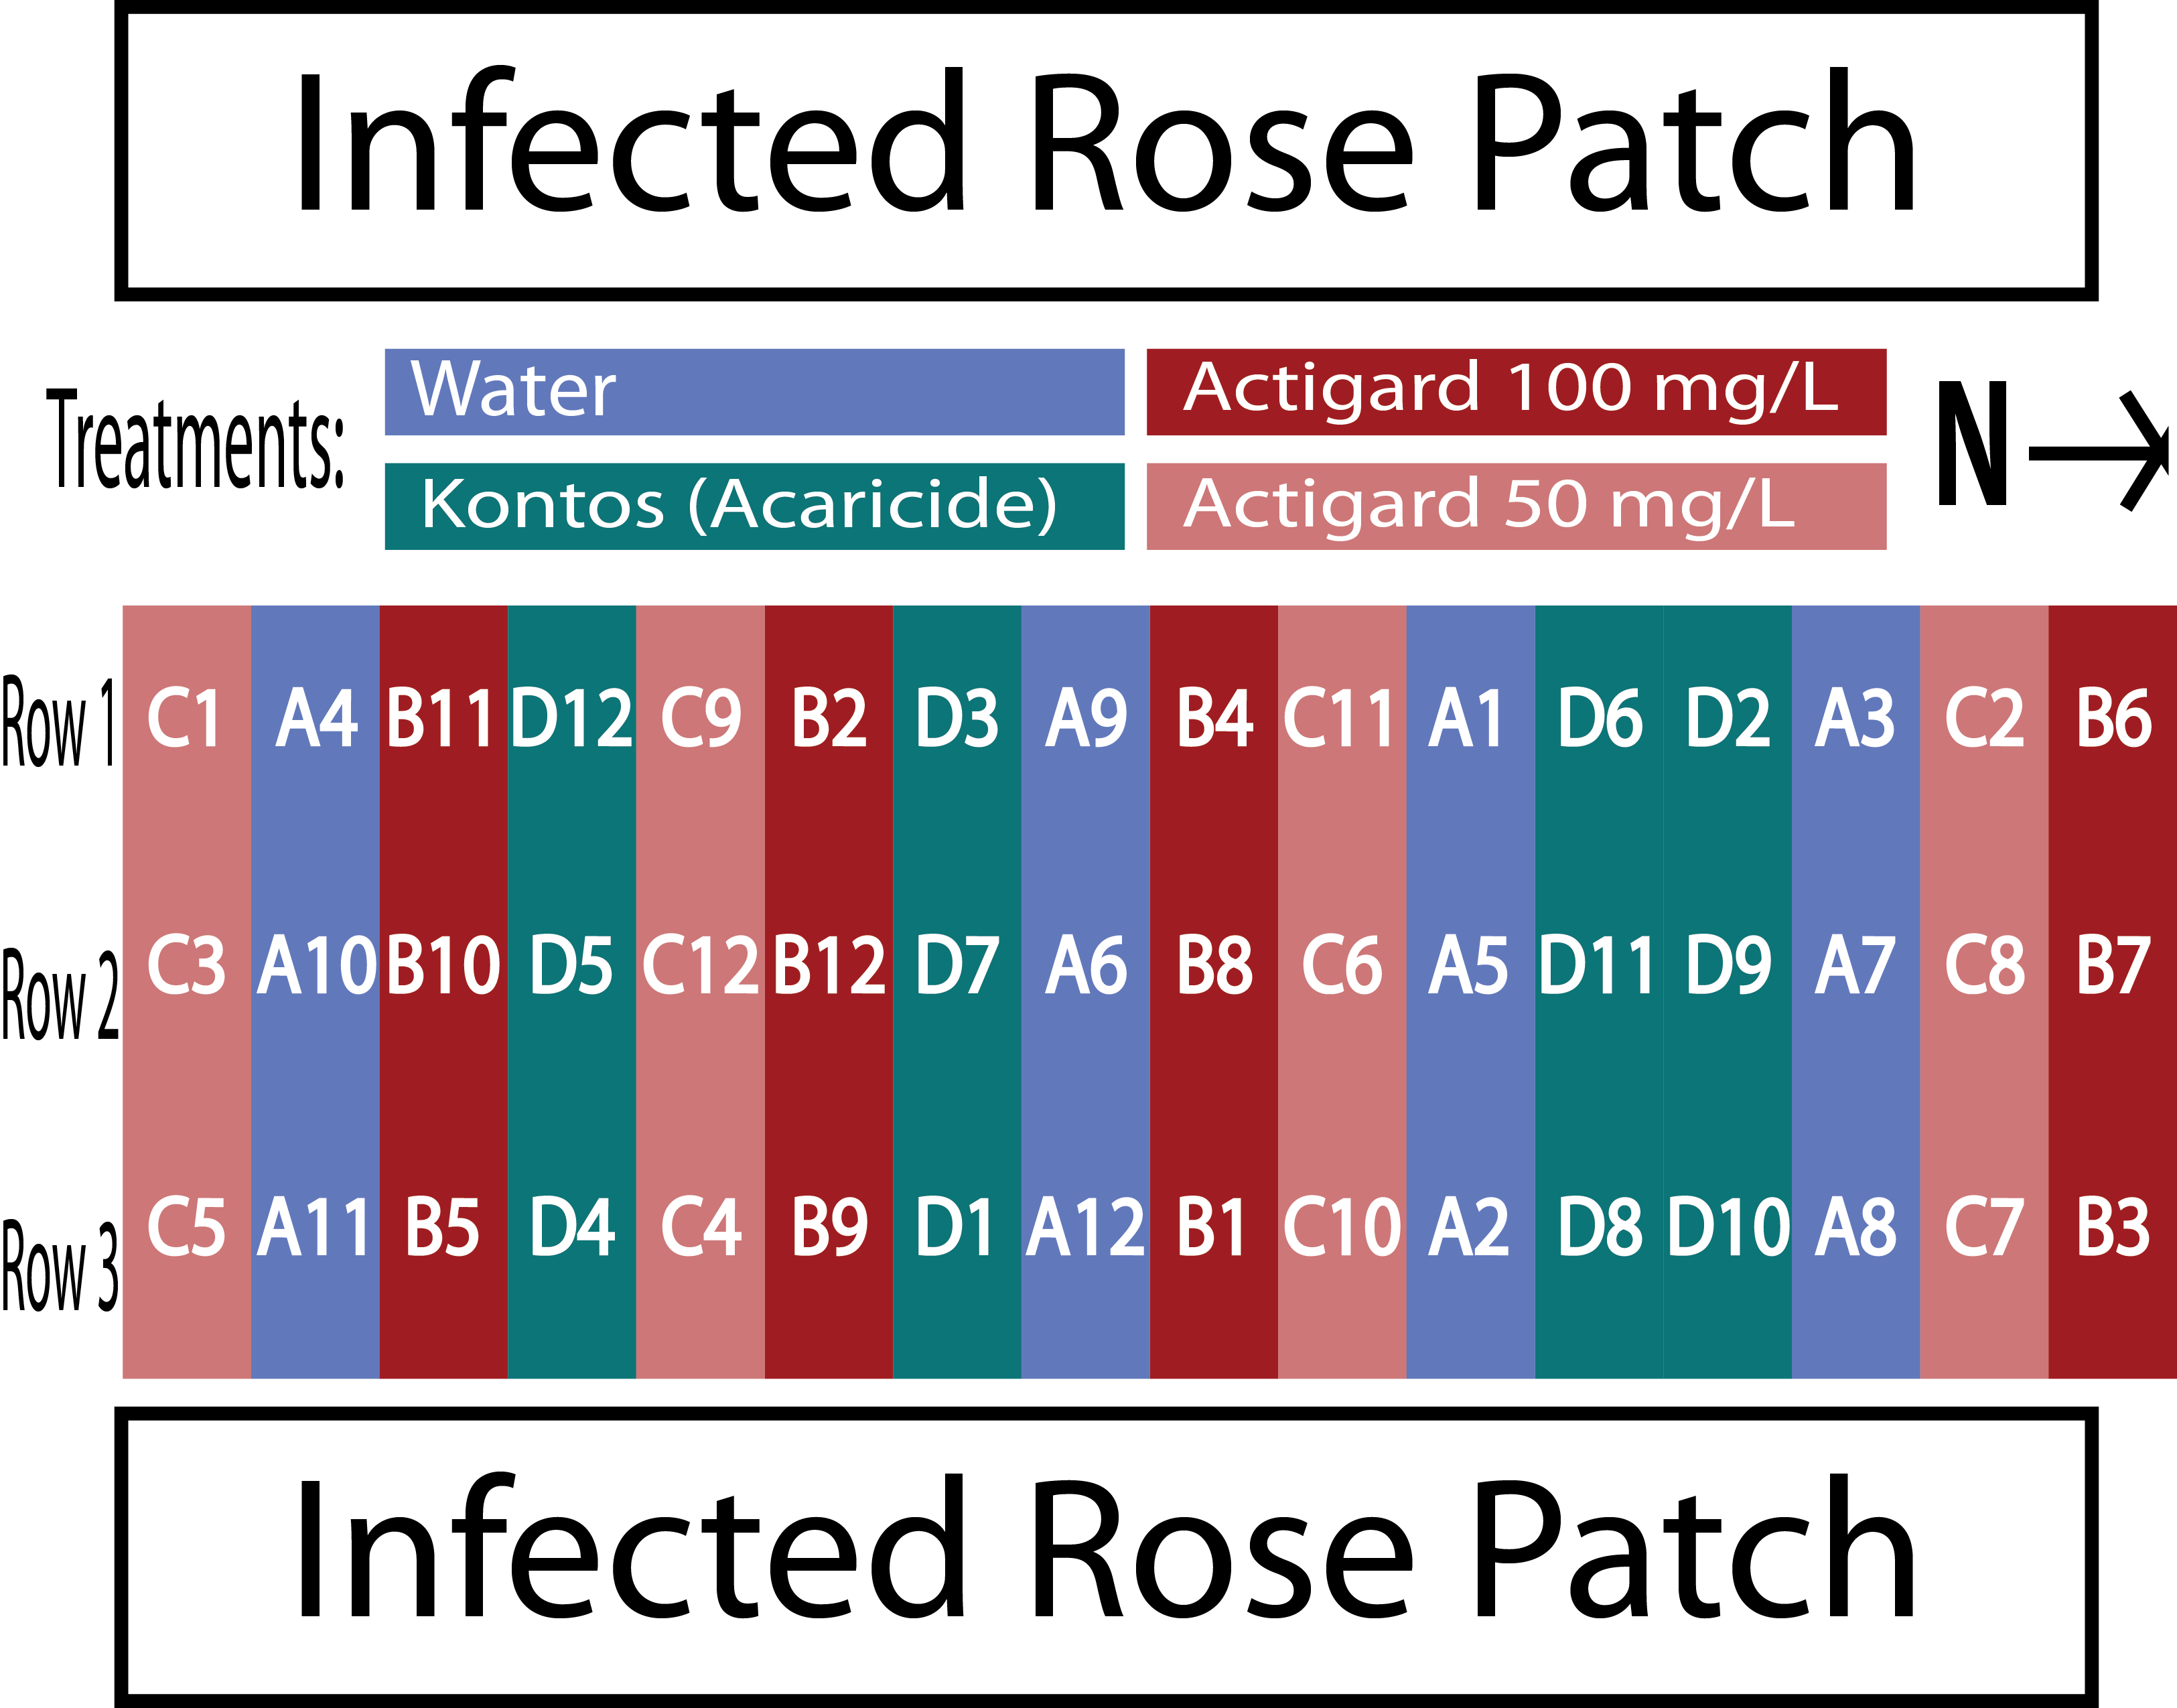
\includegraphics[width=0.8\linewidth]{figure/rrv_asm_plot_2019_griffin} \end{center}

  Figure 16: Field design for testing the potential of Acibenzolar-S-Methyl to reduce populations of \emph{P. fructiphilus} by inducing Systemic Acquired Resistance in Pink Double Knock Out® roses. Trials were conducted for three months from September to December 2019 in Griffin, GA. Four treatments were applied weekly fo 12 weeks: Blue = Water Red = Actigard50WG 100 mg/L (High rate), Pink = Actigard50WG 100 mg/L (Half rate) Turquoise = Kontos (Label rate). Flower cuttings were be taken weekly to record \emph{P. fructiphilus} numbers.

  \hypertarget{ipm-trials}{%
  \section{\texorpdfstring{4.2 Integrating Pest Management Methods to control \emph{Phyllocoptes fructiphilus}}{4.2 Integrating Pest Management Methods to control Phyllocoptes fructiphilus}}\label{ipm-trials}}

  \hypertarget{problem-statement-3}{%
  \subsubsection{4.2.1 Problem Statement}\label{problem-statement-3}}

  \hypertarget{proposal-we-propose-testing-various-pest-management-treatments-including-predatory-mites-to-reduce-populations-of-phyllocoptes-fructiphilus}{%
  \subsubsection{\texorpdfstring{4.2.2 Proposal: We propose testing various pest management treatments including predatory mites to reduce populations of \emph{Phyllocoptes fructiphilus}}{4.2.2 Proposal: We propose testing various pest management treatments including predatory mites to reduce populations of Phyllocoptes fructiphilus}}\label{proposal-we-propose-testing-various-pest-management-treatments-including-predatory-mites-to-reduce-populations-of-phyllocoptes-fructiphilus}}

  We propose testing two different SAR-inducers as well as predatory mites for their ability to reduce populations of \emph{P. fructiphilus}. We also intend to combine the effects of predatory mites with a SAR-inducer to determine if these treatments are compatible. All testing will be done in areas with high pest pressure in Georgia. Our hypothesis is that there will be fewer \emph{P. fructiphilus} on plants treated with the SAR-inducers when compared to the water treated control group, and even fewer mites found on plants treated with the combination of a SAR-inducer and predatory mites.

  \hypertarget{materials-methods-4}{%
  \subsubsection{4.2.3 Materials \& Methods}\label{materials-methods-4}}

  Our studies are designed to investigate if predatory phytoseiid mites such as \emph{A. swirskii} can be combined with roses' natural systemic activated resistance (SAR) to manage populations of the plant-parasitic mite, \emph{P. fructiphilus}, the vector of Rose Rosette Virus (RRV). Our findings will be used to develop Integrated Pest Management (IPM) programs for \emph{P. fructiphilus} management.

  \textbf{Roses}
  This will be a 12-week experiment conducted from August to October simultaneously in Griffin, GA and Athens, GA.
  The Athens site will be given 96 Pink Double Knock Out® Roses (Star Roses and Plants, West Grove, PA, USA), while Griffin will use 54 roses due to the smaller plot area available. Bare root roses will be planted 2 months before the trials begin to allow new flush to form. Rose planting media and environmental conditions will be the same as previously described.

  \textbf{Mite Infestation}
  \emph{Phyllocoptes fructiphilus} are present in the landscape of Georgia. Rose cuttings \textasciitilde10 cm will be taken from roses showing symptoms of Rose Rosette Disease in the landscape and placed in each rose pot on the 1st, 5th and 9th week of the experiment.

  \textbf{Predatory mites}

  \emph{Amblyseius swirskii} mites will be applied on the 1st, 5th and 9th week of the experiment. These mites are deployed from polyethylene fiber sachets containing live colonies of \emph{A. swirskii} and a mite which they consume for food. There is a small hole at the bottom of these sachets which allows the mites to be slowly released into the environment.

  \textbf{Field Treatments}
  \begin{enumerate}
  \def\labelenumi{\arabic{enumi}.}
  \tightlist
  \item
    Water - Control
  \item
    Actigard - 100 mg/L
  \item
    Ninja - label rate
  \item
    Kontos - label rate
  \item
    \emph{A. swirskii} (one sachet per rose treated)
  \item
    \emph{A. swirskii} + Ninja (one sachet per rose treated, label rate)
  \end{enumerate}
  \textbf{Data Collection}

  Georgia collaborators will be collecting flower samples from all roses once before beginning the treatments on week 1 and once at the end of the experiment on week 12. For weeks 2 through 11, Georgia collaborators will collect flower samples starting from the top rows of each block every week, until each row has been sampled three times (see \emph{Figure 17} and \emph{Figure 18}). Georgia collaborators rate disease severity for each rose every week before they spray, rating roses according to the Horsfall-Barratt Scale (Horsfall 1945). Roses displaying symptoms of RRD will have tissues sent to the Plant Disease Diagnostic Clinic at the North Florida Reasearch and Extension Center(PDC) for virus confirmation.

  \textbf{Sample Processing}
  \begin{itemize}
  \tightlist
  \item
    A flower cutting of about \textasciitilde12 cm will be take and placed the flower petal side down into 50 ml centrifuge tubes filled with 15 ml of 95\% ethanol so the entire flower is submerged over the sepals. Once the lid is is secure, the the tube will be shaken vigorously for a few seconds to help dislodge any mites. Samples will be processed using the washing methods of Monfreda et al. (2007), eriophyoid mites will be counted and identified as previously described.
  \end{itemize}
  \textbf{Plot Design - Athens}

  The site at Athens, GA has space for five blocks: A, B, C, D and E. Each block is a 3 \(\times\) 6 plot with 18 plants, with three plants in each treatment. The experiments will be run for 12 weeks. We will be sampling flower cuttings from two rows each week, starting with the top rows (1-15 and 16-30 for week one) of each block and rotating to the next row each week (31-45 and 46-60 on week 2) continuing until all rows have been sampled three times. In order to avoid confusion, each rose pot will be labeled with a stake that has the plant number and treatment abbreviation: (W, A, K, M, N, +) written on it. Applications will be done on the same day each week, weather permitting, preferably at the beginning of the week.
  \begin{center}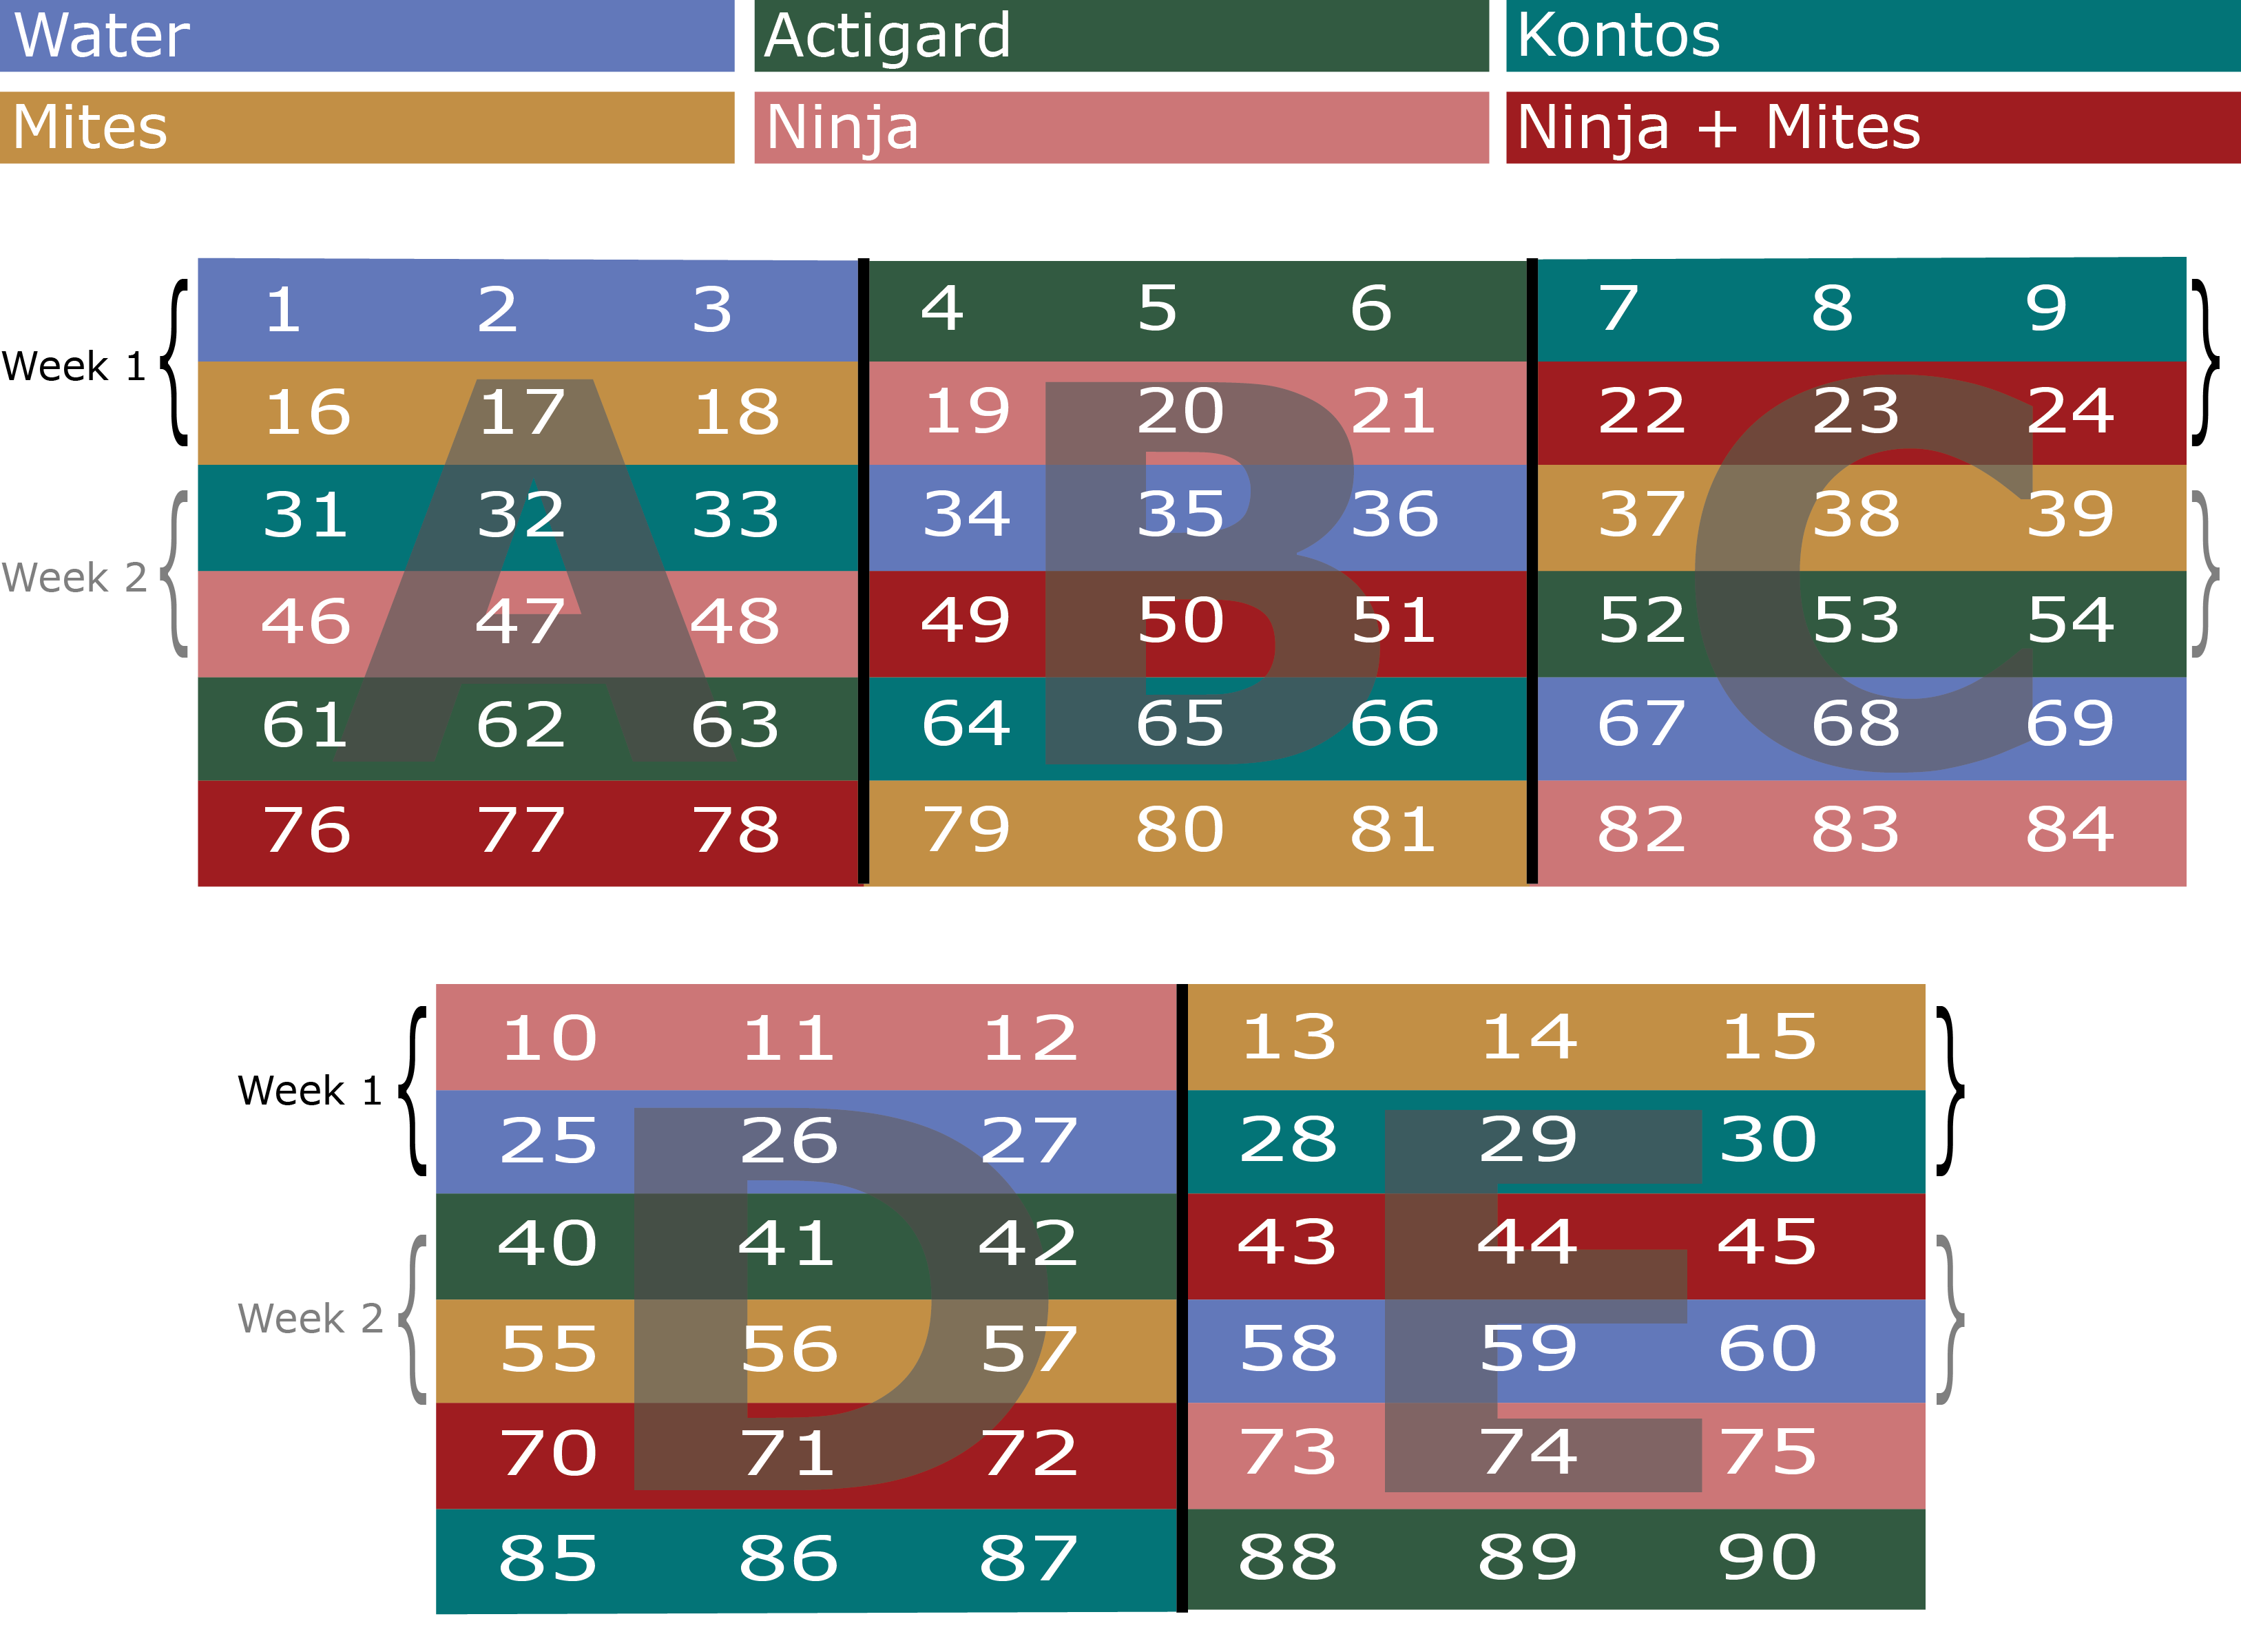
\includegraphics[width=0.8\linewidth]{figure/rrv_ipm_plot_map_2019_athens} \end{center}

  Figure 17: Field design for Integrated Pest Management trials on Pink Double Knock Out® roses to control \emph{P. fructiphilus} in Athens, GA with five treatments. W = Water A = Actigard50WG, K = Kontos, M = \emph{A. swirkii} predatory mite sachets, N = SP2700 (Trade name: Ninja, SePro), + = \emph{A. swirskii} + Ninja combined treatments. All products were applied at their label rates for 12 weeks. Flower cuttings were taken weekly to record \emph{P. fructiphilus} numbers.

  \textbf{Plot Design - Griffin}

  The site at Griffin, GA has space for three blocks: X, Y, and Z. Each block is a 3 \(\times\) 6 plot with 18 plants, with three plants in each treatment. This experiment was run for 12 weeks as well. We will be sampling flower cuttings from two rows each week, starting with the top rows (1-9 and 10-18 for week one) of each block and rotating to the next row each week (19-27 and 28-36 on week 2) continuing until all rows have been sampled three times. Labels and applications were conducted in the same manner as previously described.
  \begin{center}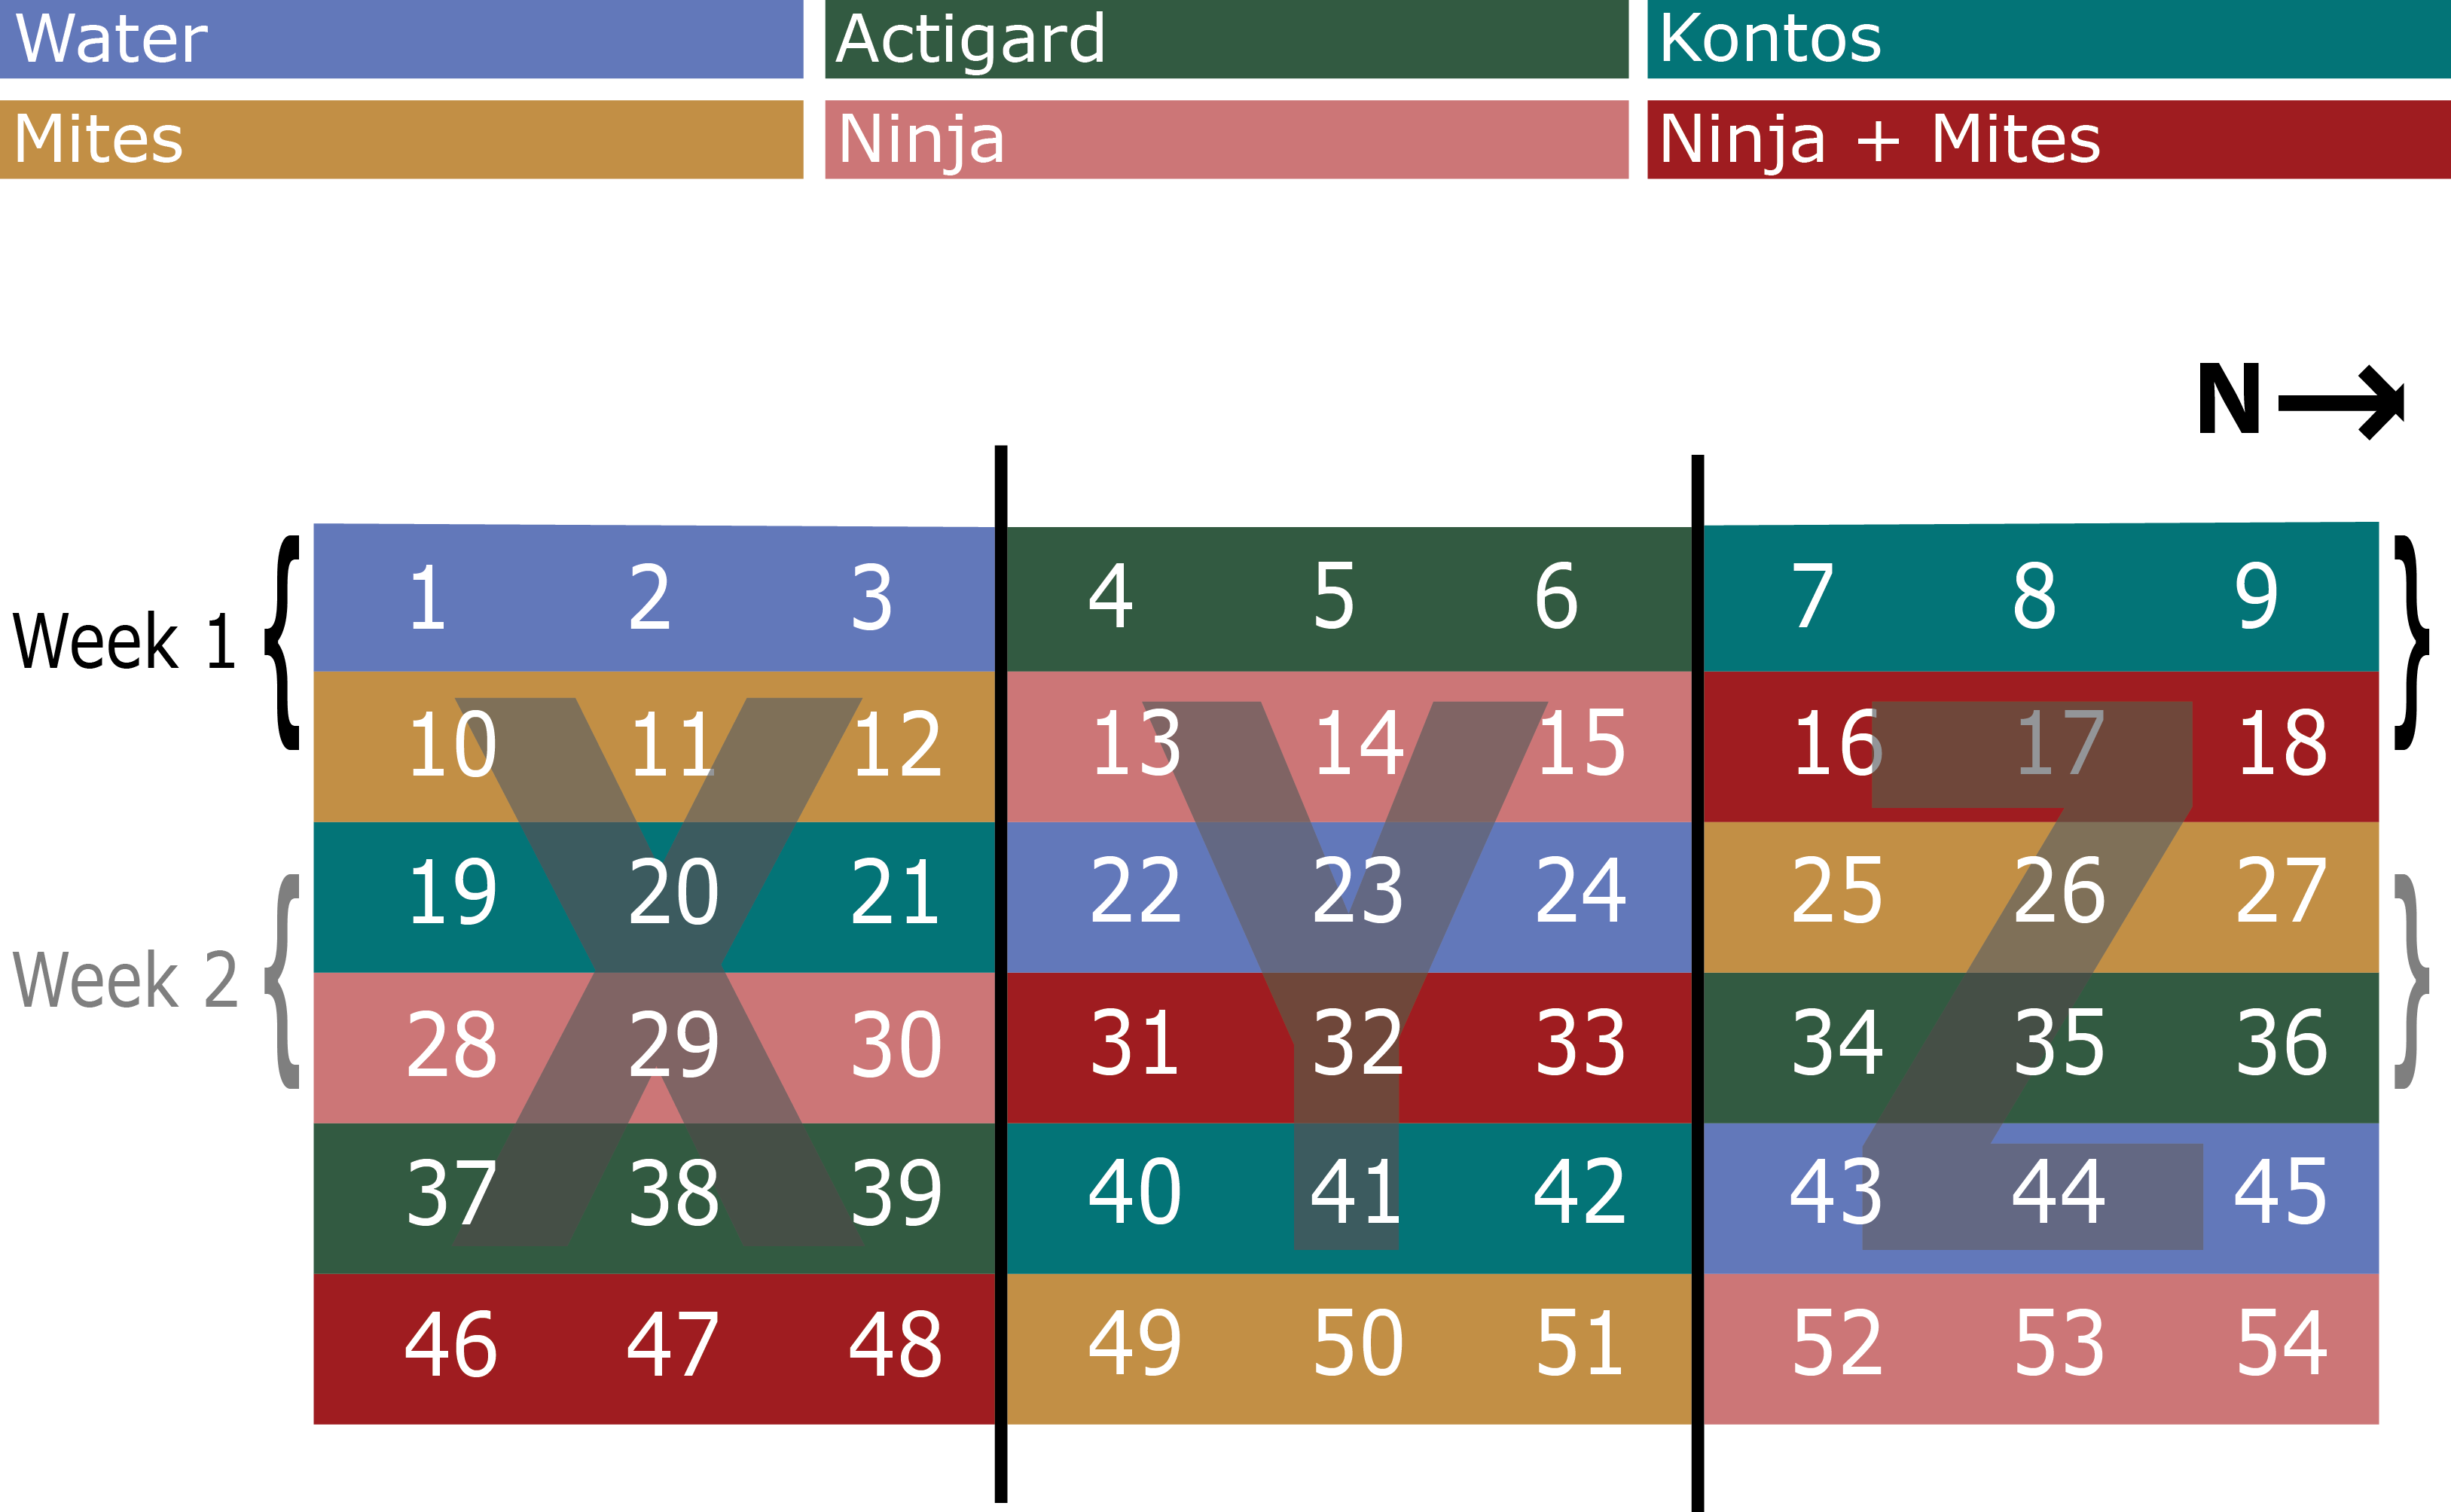
\includegraphics[width=0.8\linewidth]{figure/rrv_ipm_plot_map_2019_griffin} \end{center}

  Figure 18: Field design for Integrated Pest Management trials on Pink Double Knock Out® roses to control \emph{P. fructiphilus} in Griffin, GA with five treatments. W = Water A = Actigard50WG, K = Kontos, M = \emph{A. swirkii} predatory mite sachets, N = SP2700 (Trade name: Ninja, SePro), + = \emph{A. swirskii} + Ninja combined treatments. All products were applied at their label rates for 12 weeks. Flower cuttings were taken weekly to record \emph{P. fructiphilus} numbers.
  \begin{center}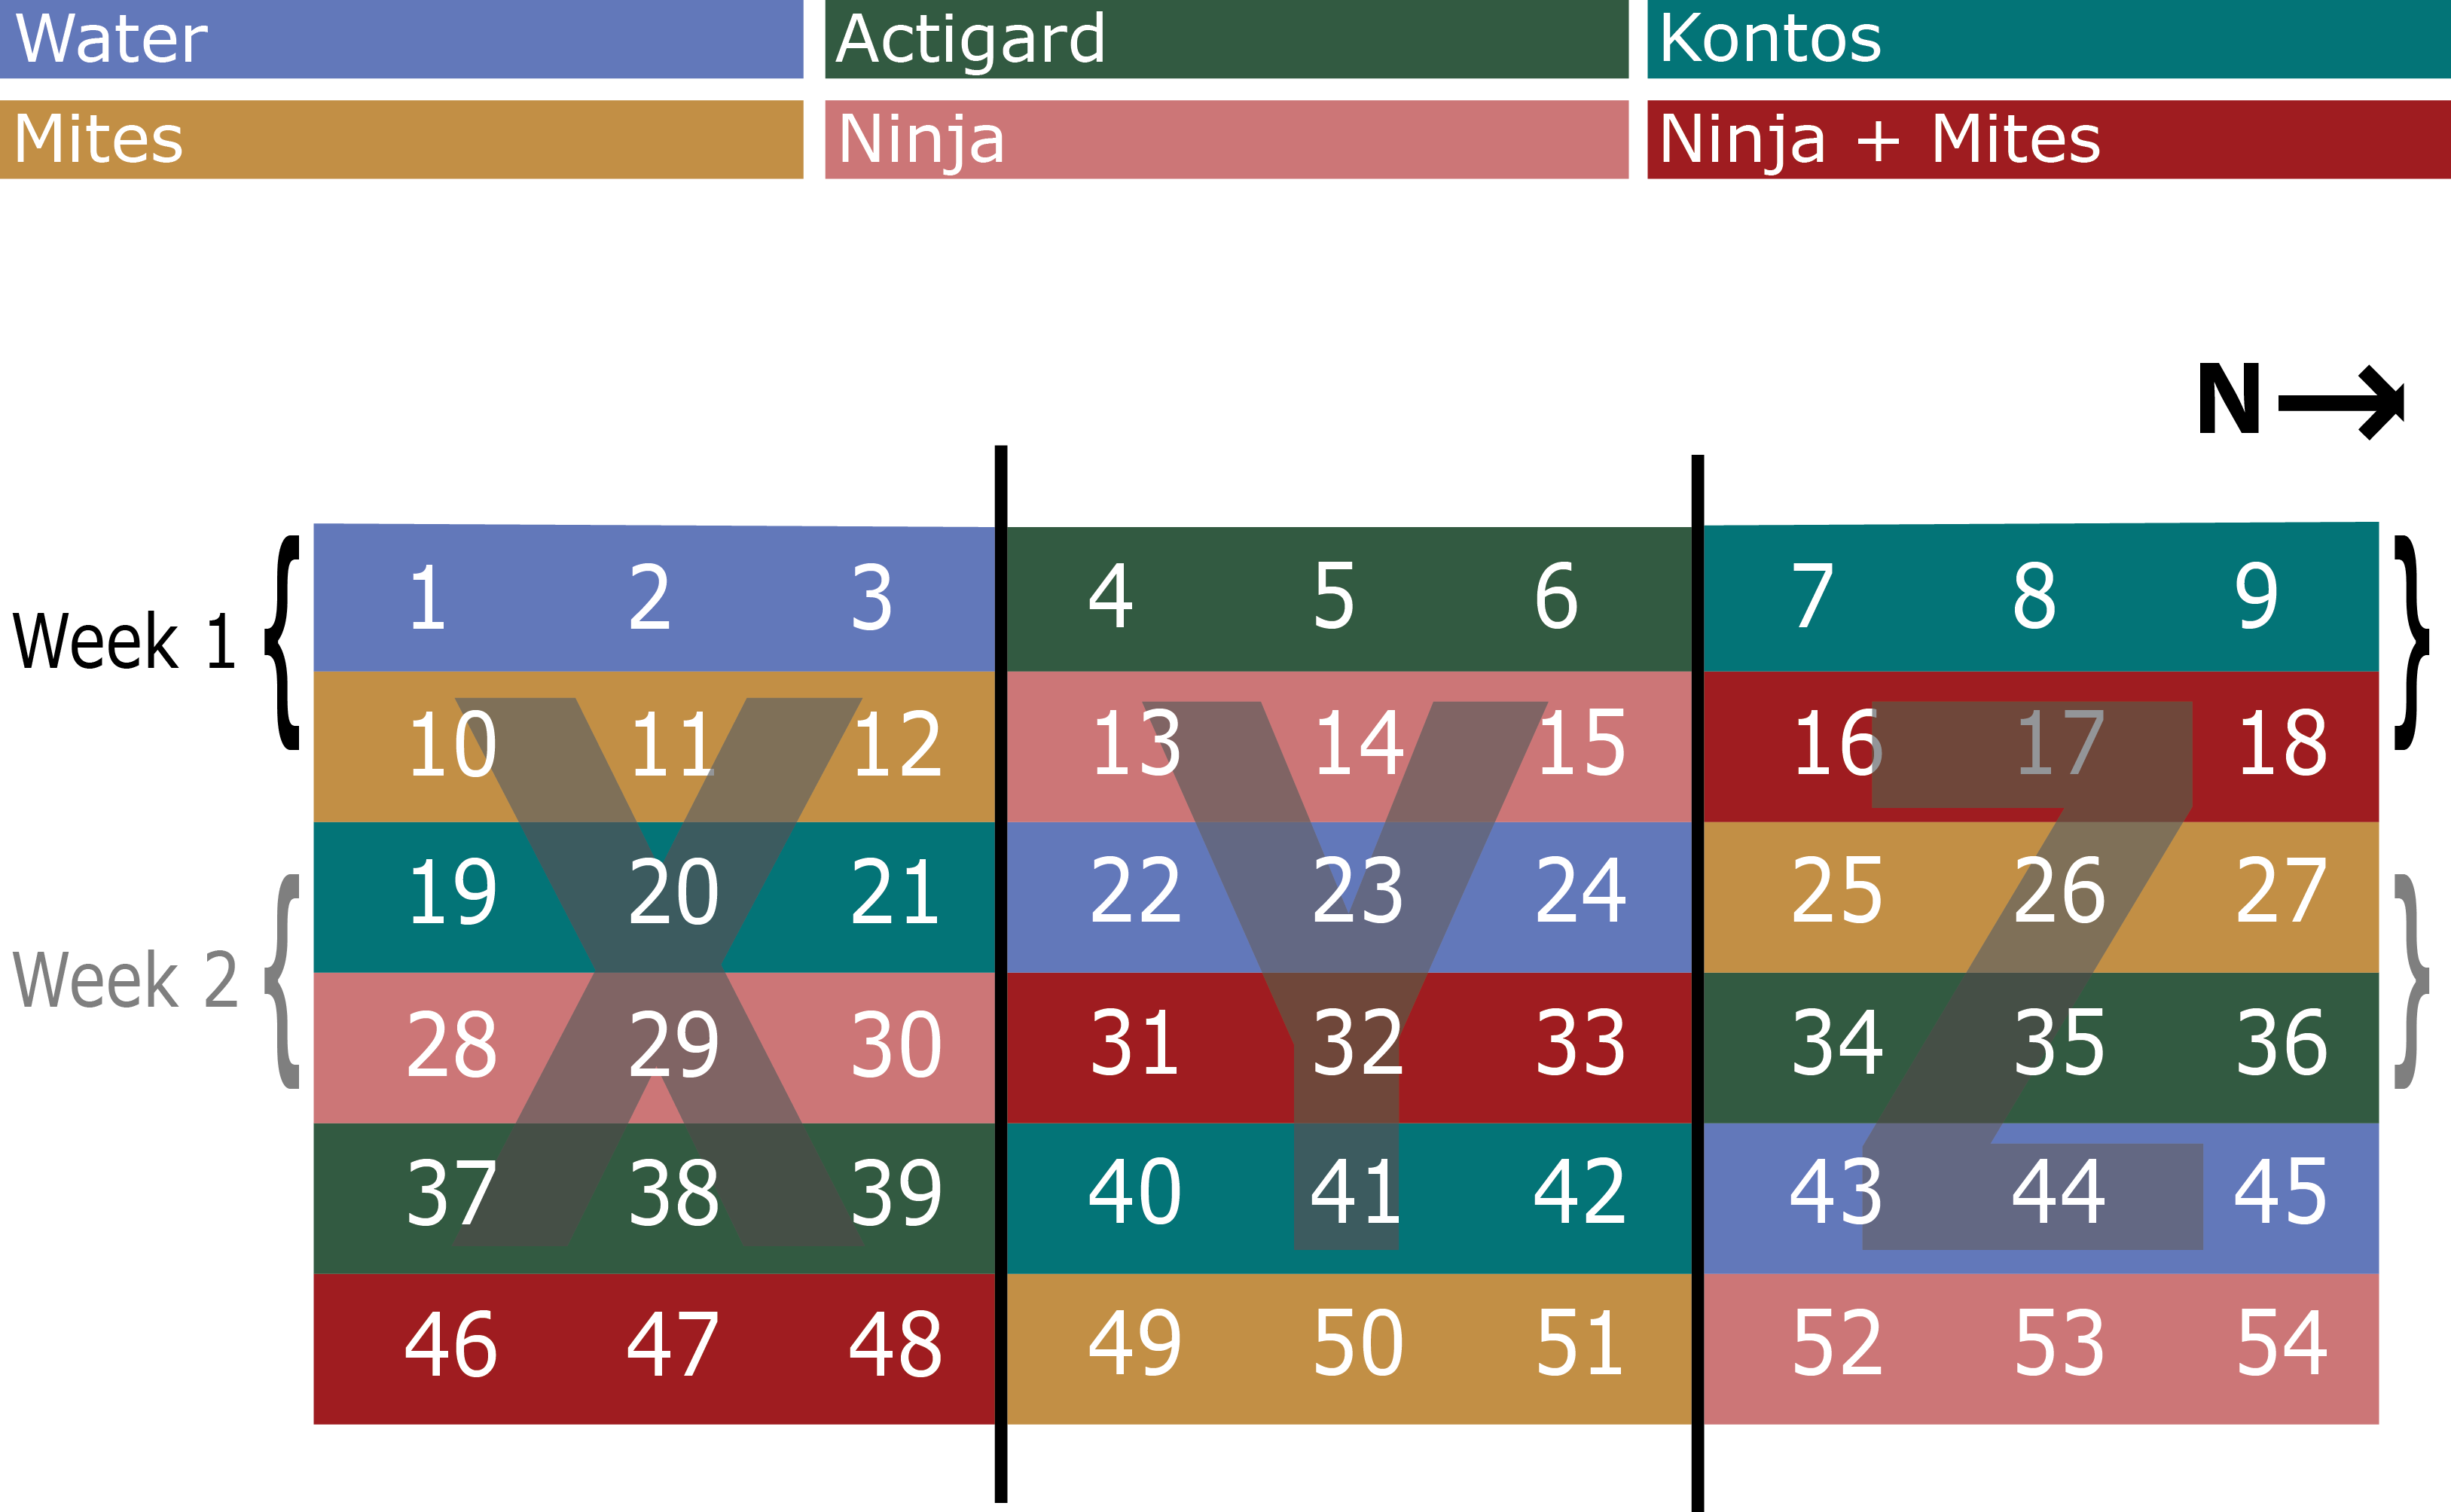
\includegraphics[width=0.8\linewidth]{figure/rrv_ipm_plot_map_2019_griffin} \end{center}

  Figure 19: Field design for Integrated Pest Management trials on Pink Double Knock Out® roses to control \emph{P. fructiphilus} in Tallahassee, FL with five treatments: Water, Actigard50WG, Kontos, \emph{Amblyseius swirkii} predatory mite sachets, and \emph{A. swirskii} + Actigard combined treatments. All products were applied at their label rates for 12 weeks. Flower cuttings were taken weekly to record \emph{P. fructiphilus} numbers.
  \begin{center}
\includegraphics[width=0.8\linewidth]{figure/reed} \end{center}

  Figure 20: Number of \emph{Phyllocoptes fructiphilus} found in rose samples with five treatments. Statistical significance was determined using Tukey contrasts for multiple Comparisons of means. Groups which share letters are not statistically different from one another. a = 0.05

  \hypertarget{brevipalpus-transmitted-orchid-fleck-virus-infecting-three-new-ornamental-hosts-in-florida}{%
  \subsection{\texorpdfstring{\emph{Brevipalpus}-transmitted orchid fleck virus infecting three new ornamental hosts in Florida}{Brevipalpus-transmitted orchid fleck virus infecting three new ornamental hosts in Florida}}\label{brevipalpus-transmitted-orchid-fleck-virus-infecting-three-new-ornamental-hosts-in-florida}}

  Austin \textbf{Fife}\textsuperscript{1}, Daniel \textbf{Carrillo}\textsuperscript{2}, Gary \textbf{Knox}\textsuperscript{3}, Fanny \textbf{Iriarte}\textsuperscript{4}, Kishore \textbf{Dey}\textsuperscript{5}, Avijit \textbf{Roy}\textsuperscript{6}, Ronald \textbf{Ochoa}\textsuperscript{7}, Gary \textbf{Bauchan}\textsuperscript{8}\(\dagger\), Mathews \textbf{Paret}\textsuperscript{4,9}, Xavier \textbf{Martini}\textsuperscript{1}*

  \textsuperscript{1} University of Florida, Department of Entomology and Nematology, North Florida Research and Education Center, Quincy FL 32351

  \textsuperscript{2} University of Florida, Department of Entomology and Nematology, Tropical Research and Education Center, Homestead FL 33031

  \textsuperscript{3} University of Florida, Department of Environmental Horticulture, North Florida Research and Education Center, Quincy FL 32351

  \textsuperscript{4} University of Florida, Department of Plant Pathology, North Florida Research and Education Center, Quincy FL 32351

  \textsuperscript{5} The Florida Department of Agriculture and Consumer Services, Division of Plant Industry, Section of Plant Pathology, Doyle Conner Building, 1911 SW 34th street, Gainesville, FL 32608

  \textsuperscript{6} United States Department of Agriculture -- Agriculture Research Service, Molecular Plant Pathology Laboratory, 10300 Baltimore Ave, Bldg. 4 BARC-West, Beltsville, MD 20705

  \textsuperscript{7} United States Department of Agriculture - Agriculture Research Service, Systematic Entomology Laboratory 10300 Baltimore Ave, Bldg. 5 BARC-West, Beltsville, MD 20705

  \textsuperscript{8} United States Department of Agriculture - Animal and Plant Health Inspection Service, Electron and Confocal Microscopy Unit, Bldg. 12 BARC-West, 10300 Baltimore Ave, Beltsville, MD 20705

  \textsuperscript{9} Plant Pathology Department, University of Florida, Gainesville, FL 32611

  *Corresponding author; E-mail: xmartini@ufl.edu Phone: 850-875-7160 Fax: 352-846-6617

  \pagebreak

  \hypertarget{abstract}{%
  \subsection{Abstract}\label{abstract}}

  We describe the first detection of orchid fleck virus (OFV) infecting three unreported hosts: \emph{Liriope muscari}, cv. `Gigantea' (Decaisne) Bailey, \emph{Ophiopogon intermedius} Don and \emph{Aspidistra elatior} Blume (Asparagaceae: Nolinoidaea) in Leon and Alachua Counties, FL. The orchid-infecting subgroup (Orc) of OFV infects over 50 plant species belonging to the plant families Orchidaceae, Asparagaceae (Nolinoidaea), and causes citrus leprosis disease in \emph{Citrus} (Rutaceae). The only known vectors of OFV-Orc are the flat mites, \emph{Brevipalpus californicus} (Banks) \emph{sensu lato} (Trombidiformes: Tenuipalpidae). Florida has various plants in the landscape which \emph{Brevipalpus} spp. feed on, which are susceptible to infection by OFV-Orc. Chlorotic ringspots and flecking were seen affecting Liriopogons (\emph{Liriope} and \emph{Ophiopogon} spp.) in Leon County, FL. Nearby \emph{A. elatior} also appeared chlorotic. Local diagnostics returned negative for common plant pathogens, therefore new samples were sent to the Florida Department of Agriculture and Consumer Services (FDACS) and USDA-ARS for identification. Two orchid-infecting strains of OFV were detected via combinations of conventional RT-PCR, RT-qPCR, Sanger sequencing and High Throughput Sequencing (HTS). Amplicons shared 98\% nucleotide identity with OFV-Orc1 and OFV-Orc2 RNA2 genome sequences available in NCBI GenBank. Coinfections were detected in each county, but single strains of OFV-Orc were detected in \emph{L. muscari} (Alachua, OFV-Orc2) and \emph{A. elatior} (Leon, OFV-Orc1). Three potential mite vectors were identified via cryo-scanning electron microscopy (Cryo-SEM): \emph{Brevipalpus californicus} (Banks) sensu lato, \emph{B. obovatus} Donnadieu, and \emph{B. confusus} Baker. In conclusion, OFV orchid strains are present in northern Florida, representing a risk for susceptible plants in the southeastern US.

  \hypertarget{resumen}{%
  \subsection{Resumen}\label{resumen}}

  Se describe la primera detección del virus de orchid fleck virus (OFV), infectando a tres huéspedes no reportados: \emph{Liriope muscari}, cv. `Gigantea' (Decaisne) Bailey, \emph{Ophiopogon intermedius} Don and \emph{Aspidistra elatior} Blume (Asparagaceae: Nolinoidaea) para los condados de Leon y Alachua, FL. Los subgrupos de OFV que infectan a las orquídeas (Orc) puedan infectar más de 50 especies de plantas pertenecientes a las familias Orchidaceae, Asparagaceae (Nolinoidaea), e infecta \emph{Citrus} (Rutaceae) cómo la enfermedad de la leprosis de los cítricos. Los únicos vectores de OFV-Orc son los ácaros planos \emph{Brevipalpus californicus} (Banks) \emph{sensu lato} (Trombidiformes: Tenuipalpidae). La Florida tiene varias plantas en el campo ornamental, por lo cúales las especias de \emph{Brevipalpus} se puedan alimentarse, y esas plantas son susceptibles a las infecciones de OFV-Orc. Se observaron manchas anulares cloróticas y salpicaduras en las hojas de las Serpentinas (\emph{Liriope} y \emph{Ophiopogon} spp.) y también se vieron hojas cloróticas en el \emph{A. elatior} adyacente, situado en el condando de Leon, FL. Los diagnósticos del laboratorio local fueron negativos para los patógenos comunes, por lo tanto, se enviaron nuevos ejemplares al Florida Department of Agriculture and Consumer Services (FDACS) y el USDA-ARS para su identificación. Se detectaron dos cepas del OFV mediante la combinación de RT-PCR convencional, RT-qPCR, secuenciación de Sanger y secuenciación de alto rendimiento. Las ampliaciones compartían una identidad de nucleótidos del 98\% con las secuencias del genoma de ARN2 de OFV-Orc1 y OFV-Orc2 disponibles en el NCBI GenBank. Se detectaron coinfecciones del virus en cada condado, pero se detectaron cepas únicas de OFV-Orc en \emph{L. muscari} (Alachua , OFV-Orc2) y \emph{A. elatior} (Leon , OFV-Orc1). Se identificaron tres ácaros mediante microscopía electrónica de barrido criogénico (Cryo-SEM) con potencial de ser vectores: \emph{Brevipalpus californicus} (Banks) \emph{sensu lato}, \emph{B. obovatus} Donnadieu y \emph{B. confusus} Baker. En conclusión, OFV está presente en el norte de Florida, lo que representa un riesgo para las plantas susceptibles en el sureste de Estados Unidos.

  \hypertarget{keywords}{%
  \subsection{Keywords:}\label{keywords}}

  False spider mite, flat mite, \emph{Brevipalpus}-transmitted viruses, \emph{Liriope}, Nolinoidaea, \emph{Ophiopogon}, \emph{Aspidistra}, Ruscaceae, Rutaceae, Asparagaceae, orchid, Orchidaceae, pests, ornamental plants, orchid fleck virus.

  \pagebreak

  Orchid fleck virus (OFV), is the type member for the genus \emph{Dichorhavirus}, family \emph{Rhabdoviridae}. The virus is a bacilliform, nuclear rhabdovirus composed of two segments of single-stranded, negative-sense RNA which infects plants (Dietzgen et al. 2014, Walker et al. 2018, Amarasinghe et al. 2019). Only Flat mites (Trombidiformes: Tenuipalpidae) from the genus \emph{Brevipalpus} are known to transmit dichorhaviruses (Maeda 1998). Plants infected with OFV exhibit chlorotic and necrotic flecks on their leaves(Kubo et al. 2009b, Kubo et al. 2009a, Dietzgen et al. 2018b). The virus was first described as infecting \emph{Cymbidium} orchids in Japan (Doi et al. 1977). There have been reports of OFV and OFV-like rhabdoviruses infecting orchids in Asia, Africa, North America, South America, Europe, and Oceania. The prevalence of OFV and its mite vector is thought to be associated with the movement of infected orchids (Dietzgen et al. 2018a). More than fifty species of Orchidaceae (Kitajima et al. 2010, Peng et al. 2013) can naturally become infected with OFV, as well as some Asparagaceae (Nolinoidaea) (Mei et al. 2016, Dietzgen et al. 2018b), and Rutaceae, where infection causes citrus leprosis-like symptoms (Roy et al. 2015, 2020, Cook et al. 2019, Olmedo-Velarde et al. 2021). Mechanical transmission of OFV is possible under laboratory conditions to the plant families Chenopodiaceae, Aizoaceae, Fabaceae, and Solanaceae (Chang et al. 1976, Kondo et al. 2003, Peng et al. 2013).

  \hypertarget{virus-detection}{%
  \subsubsection{Virus Detection}\label{virus-detection}}

  During June 2020, chlorotic flecks and ringspot patterns of unknown etiology were observed on Giant Lilyturf \emph{Liriope} spp., cv. `Gigantea' in a landscape of Leon County, Florida (Figure 21). \emph{Liriope} belong to a group of plants in the family Asparagaceae, subfamily Nolinoidaea, comprised of grass-like monocotyledonous liliod plants native to southeastern Asia (Chase et al. 2009, Meng et al. 2021). \emph{Liriope} and the closely related \emph{Ophiopogon} (Asparagaceae: Nolinoidaea) are considered the most important ground cover plant in the southeastern United States (Mcharo et al. 2003). Viral infections of suspected leaf samples were initially tested at the Plant Disease Diagnostic Clinic at the North Florida Research and Education Center (NFREC) in Quincy, FL. All the samples were tested with one step conventional RT-PCR, and were found negative for begomovirus, carlavirus, potyvirus, tospovirus, cucumber mosaic virus and tobacco mosaic virus. As initial diagnostics were inconclusive, samples were taken of putatively infected plants with ringspot symptoms during July and August of 2020. Leaves were taken from \emph{Liriope} spp. and \emph{Ophiopogon} spp., as well as the \emph{Aspidistra elatior} Blume (Asparagaceae: Nolinoidaea), nearby, which appeared sickly and chlorotic (Figure 22). Plant materials were sent to the Florida Department of Agriculture and Consumer Services (FDACS) for identification. The FDACS determined that the pathogen was OFV using previously published primers and methods to conduct RT-PCR and Sanger sequencing (Kubo et al. 2009b, Kubo et al. 2009a, Ramos-González et al. 2015).
  The identity of the virus was verified as OFV Orchid strain 1, (OFV-Orc1), following the methods described in Kondo et al. (2017). Nucleotide sequencing shared 98\% nucleotide identity with the OFV-isolates So (Accession No.~AB244418) and Br (Accession No.~MK522807), which belong to orchid subgroup I (Kondo et al. 2006, 2017). These samples from FDACS were subsequently retested by the USDA-APHIS-PPQ S\&T Beltsville laboratory, in conjunction with tests of fresh samples from both Alachua and Leon counties. The USDA used RT-PCR, RT-qPCR, and High Throughput Sequencing (HTS) to reconfirm the presence of OFV. Conventional RT-PCR with Generic R2-Dicho-GF and R2-Dicho-GR primers amplified \textasciitilde800 nt amplicons of the L-gene (RNA2) (Roy et al. 2020), to detect both OFV-Orc1 and OFV-Orc2 in \emph{O. intermedius} and \emph{A. elatior} from Leon County (Kondo et al. 2017) (GenBank Accession Numbers: MZ852004, MZ852005 MZ852006, and MZ852007). 99\% nucleotide sequence identity is shared between OFV-Orc1 and OFV-Orc2 for the RNA2 genome, whereas 90\% sequence identity was found between these two reassortment strains. The presence of OFV-Orc1 and OFV-Orc2 in Leon and Alachua counties was reaffirmed with HTS data (Table 1): Analysis of HTS data from Leon County found that the symptomatic \emph{L. muscari} were coinfected with both OFV-Orc1 and OFV-Orc2, while the symptomatic \emph{A. elatior} were solely infected with OFV-Orc1. Sequence data of symptomatic \emph{L. muscari} from Alachua County revealed infections with OFV-Orc2 (GenBank Accession MZ852006). After the initial identification by FDACS of OFV-Orc, mite samples were collected from symptomatic Asparagaceae in Leon County. Most mites collected were Tenuipalpid mites (flat mites or false spider mites), a pest of ornamental plants, some of which are known to act as vectors for plant viruses (Childers et al. 2003b, Childers and Rodrigues 2011).

  \hypertarget{mite-description}{%
  \subsubsection{Mite Description}\label{mite-description}}

  Mite taxonomy is complicated by cryptic species complexes which occur in many plant-feeding groups of the Acari (Umina and Hoffmann 1999, Skoracka and Dabert 2010, Arthur et al. 2011, Skoracka et al. 2013), including tenuipalpid mites from the genus \emph{Brevipalpus} (Navia et al. 2013). The commonly used phase-contrast microscopy is insufficient to detect some diagnostic characters for separation of cryptic species, instead best practices recommend the combination of Differential Interference Contrast (DIC) Microscopy and Scanning Electron Microscopy along with molecular methods to separate cryptic species (Beard et al. 2015). The flat mites collected were initially suspected to belong to \emph{B. californicus} after inspection with phase contrast microscopy. Subsequent observation via DIC microscopy at FDACS agreed with this tentative identification. Unfortunately, the \emph{B. californicus} s.l. species group, \emph{sensu} Baker and Tuttle (1987) is suspected to contain cryptic species (Childers and Rodrigues 2011, Rodrigues and Childers 2013). New mite samples were collected from symptomatic liriopogons and \emph{A. elatior} in Leon County and sent to USDA-ARS's Electron and Confocal Microscopy Unit for analysis. Three mite species were recovered and examined under cryo-scanning electron microscopy (Cryo-SEM): \emph{B. californicus} s.l. (Figure 23), \emph{B. obovatus} Donnadieu and \emph{B. confusus} Baker. The recent report of OFV in the US is thought to be Ko et al. (1985) which describes nuclear inclusions caused by an undescribed bacilliform rhabdovirus in \emph{Brassia} orchids. The significance of this report is their description of the spoke-wheel configurations of the viral particles (Ko et al. 1985), a sign typically associated with OFV infection (Chang et al. 1976). Unfortunately, this article made no mention of mites or further investigations of the virus. The first report of OFV in the continental US was Bratsch et al. (2015), who confirmed the presence of OFV in \emph{Phalaenopsis} hybrids using Transmission Electron Microscopy of ultrathin sections of plant tissue as well as molecular sequence analysis. They also discuss the association of OFV with \emph{Brevipalpus} mites, but the authors did not make a conclusive species identification beyond suggesting that the mite vector belonged to the \emph{B. californicus} group, referring to Kondo et al. (2003)'s publication (Bratsch et al. 2015). Later reports of OFV described OFV infecting a previously undescribed Nolinoidaea hosts in Australia (Mei et al. 2016, Dietzgen et al. 2018b), including \emph{Liriope spicata} (Thunb.) Lour, a different species of liriopogon than those identified from the Florida sites. We are not aware of any reports of OFV infecting liriopogons, \emph{A. elatior} nor other Nolinoidaea in the US. Although Peng et al. (2013) had mentioned an association between \emph{B. californicus} and \emph{A. elatior}, they never reported symptoms of OFV-Orc in this plant. We believe that our findings indicate the first report of OFV-Orc infecting ornamental Nolinoidaea in Florida, and possibly the US. This publication also marks the first reports of \emph{A. elatior} and \emph{Ophiopogon} spp. as natural hosts of OFV-Orc. There are two orchid strains of OFV (OFV-Orc1 and OFV-Orc2), and two citrus strains (OFV-Cit1 and OFV-Cit2) (Beltran-Beltran et al. 2020, Roy et al. 2020). The OFV strains detected in Florida are identical in genome sequence to the orchid strains of OFV infecting citrus in Hawaii, Mexico, Colombia, and South Africa (Beltran-Beltran et al. 2020, Roy et al. 2020). Both OFV-Orc1 and OFV-Orc2 infect citrus (Roy et al. 2020), but none of the citrus strains have been reported from any orchid species. The \emph{Brevipalpus} mites collected from liriopogons and \emph{A. elatior} in Leon County were abundant on OFV-infected plants very near to citrus trees, some plants even surrounding the trunk. \emph{B. californicus} s. l. has been reported as a pest of citrus (Childers et al. 2003b) and are often collected from citrus fruits (Baker 1949, Baker and Tuttle 1987, Vacante 2010, 2016). The proximity of these mite vectors to citrus raises the question: why these trees are not currently infected with OFV-Orc? It is important to note the uncertainty surrounding the vector for OFV-Orc. There are three mite species which have been recovered from OFV-Orc infected plants: \emph{B. obovatus}, and \emph{B. confusus} and \emph{B. californicus} s.l., but only \emph{B. californicus} has been described as a vector of OFV. Even so, the \emph{B. californicus} which we find on liriopogons and \emph{A. elatior} may not be the same cryptic species as those found on citrus. Transmission of OFV from populations of \emph{B. californicus} liriopogon/\emph{A. elatior} to citrus may be limited by host preferences, vectorial capacity, viral propagation/circulation in the vector, viral acquisition times, or feeding times required for transmission to citrus. Even so, these types of questions require future study to determine the potential of nolinoidaea to citrus transmission. Best practices for integrated pest management have not been created for controlling \emph{Brevipalpus} mites on these ornamentals, but methods designed to control \emph{Brevipalpus} in other systems may be applicable. The most common method used to control \emph{Bervipalpus} are synthetic acaricides (Andrade et al. 2010, 2019). Unfortunately, some acaricides and their residues can harm beneficial predatory mites as well (Fernández et al. 2017), even at low doses (Havasi et al. 2021), and mixing different chemistries can be detrimental for mite control (Vechia et al. 2018). In addition, pesticide resistance has been reported in various \emph{Brevipalpus} populations (Alves et al. 2000, Omoto et al. 2000, Campos and Omoto 2002, Rocha et al. 2021), due to exposure to pesticides used to control other arthropod pests (Vechia et al. 2021). In addition, predatory mites (Chen et al. 2006, Argolo et al. 2020), entomopathogenic fungi (Magalhães et al. 2005, Rossi-Zalaf et al. 2008, Peña et al. 2015, Revynthi et al. 2019) have shown promise for controlling other \emph{Brevipalpus} mites. Moreover, it is often possible to integrate different control techniques for improved management, such as combining predatory mites with compatible acaricides and entomopathogenic fungi (Reddy 2001, Midthassel et al. 2016, Andrade et al. 2019). In conclusion, detecting OFV in Florida represents a concern for horticulturists who grow orchids, \emph{Liriope}, \emph{Ophiopogon}, or other susceptible Asparagaceae species which are commonly used in landscaping. Florida is also home to a plethora of native and naturalized orchid species, many of which are threatened, including cultivated \emph{Vanilla} in southern Florida (Chambers et al. 2019) and the famous Ghost Orchid, {[}\emph{Dendrophylax lindenii} (Lindl.) Benth. ex Rolfe{]}. Citrus leprosis was present in Florida during the 1860's and almost eradicated by the mid-1960s (Knorr 1968, Knorr et al. 1968, Childers et al. 2003b). An examination of herbarium specimens of Florida citrus found that this historical virus, Citrus leprosis dichorhavirus-N0, is distantly related to the modern isolates of OFV (Kitajima et al. 2011, Hartung et al. 2015, Roy et al. 2020). The recent detection of OFV-Orc1 in South Africa (Cook et al. 2019) in \emph{C. sinensis} (Navel and Valencia orange) and OFV-Orc2 in Hawaii (Olmedo-Velarde et al. 2021) in \emph{C. reticulata} (mandarin) and \emph{C. jambhiri} (rough lemon) associated with leprosis-like symptoms highlights the potential threat of different isolates of OFV on citrus, which will be a definite concern to the US multi-billion-dollar citrus industry already impacted by the Huanglongbing disease. \emph{B. californicus}, \emph{B. yothersi}, and \emph{B. obovatus} are all present in Florida (Childers et al. 2003b, Akyazi et al. 2017), and are difficult to identify by non-experts, or without advanced methodologies. DNA barcoding (Armstrong and Ball 2005) or a similarly simple and accurate method for identification of these mite complexes is vital to identify mite populations which need to be monitored or controlled. By doing so, we can determine the risk OFV-Orc represents for the native plants, agriculture and the ornamental/landscaping industries of Florida and the surrounding regions.

  \hypertarget{acknowledgements}{%
  \subsection{Acknowledgements}\label{acknowledgements}}

  We would like to give special thanks for the Tallahassee Museum and their patience, cooperation, and support with collecting plant samples. We are grateful for the USDA-APHIS PPQ Beltsville laboratory for their support in the identification and confirmation OFV isolates, as well as \emph{Brevipalpus} mite identification at the USDA-ARS. We also want to thank Drs. Sam Bolton, FDACS and Aline Tassi, Univ. of Sao Paulo, Brazil for checking the mites we have sent for species validation. Furthermore, we are grateful for Dr.~Marc S. Frank's identification of the Liriopogons collected. We are especially indebted to the late Dr.~Gary Bauchan for his contributions to this study and the field of acarology, he will be greatly missed. This research was partly funded by the USDA National Institute of Food and Agriculture, Hatch project FLA-NFC-005607. Mention of trade names or commercial products in this publication is solely for the purpose of providing specific information and does not imply recommendation or endorsement by the USDA; USDA is an equal opportunity provider and employer.

  \hypertarget{table-1-list-of-asparagaceae-nolinoidaea-species-infected-with-orchid-fleck-virus-collected-from-the-landscape-of-northern-florida}{%
  \subsection{Table 1: List of Asparagaceae (Nolinoidaea) species infected with orchid fleck virus, collected from the landscape of northern Florida}\label{table-1-list-of-asparagaceae-nolinoidaea-species-infected-with-orchid-fleck-virus-collected-from-the-landscape-of-northern-florida}}
  \begin{longtable}[]{@{}
    >{\raggedright\arraybackslash}p{(\columnwidth - 6\tabcolsep) * \real{0.30}}
    >{\raggedright\arraybackslash}p{(\columnwidth - 6\tabcolsep) * \real{0.38}}
    >{\raggedright\arraybackslash}p{(\columnwidth - 6\tabcolsep) * \real{0.15}}
    >{\raggedright\arraybackslash}p{(\columnwidth - 6\tabcolsep) * \real{0.18}}@{}}
  \toprule
  Scientific Name & Common Names & County & Strains Detected \\
  \midrule
  \endhead
  \emph{Liriope muscari} cv. `Gigantea'* (Decaisne) Bailey & Lilyturf, Orchardgrass, Monkeygrass & Alachua \& Leon & OFV-Orc1 \& OFV-Orc2 \\
  \emph{Ophiopogon intermedius}** Don & Aztec Grass, `Argenteomarginatus' & Leon & OFV-Orc1 \& OFV-Orc2 \\
  \emph{Aspidistra elatior} Blume & Cast Iron Plant, Bar-room Plant & Leon & OFV-Orc1 \& OFV-Orc2 \\
  \bottomrule
  \end{longtable}
  Table 1: * \emph{Liriope muscari} cv. `Gigantea' has been traditionally classified as \emph{L. gigantea} Hume by Broussard (2007) and Fantz et al. (2015), although this distinction has been challenged by Wang et al. (2014) and Masiero et al. (2020). * * \emph{O. intermedius} is sometimes misclassified as \emph{Liriope muscari} `Variegated Evergreen Giant' Fantz (2009) or `Grandiflora White' (Fantz 2009). Both OFV-Orc1 and OFV-Orc2 were detected in each species tested, many plants were coinfected with both strains, see `\protect\hyperlink{virus-detection}{Virus Detection}.'

  \hypertarget{figure-captions}{%
  \subsection{Figure captions}\label{figure-captions}}

  Figure 21: Variety of symptoms seen on \emph{Liriope} spp. infected with orchid fleck virus (OFV): (a) symptoms on \emph{Liriope muscari} cv. `Gigantea' (b-c) Details of symptoms on \emph{L. muscari} cv. `Gigantea' (d) rust colored spots on \emph{Ophiopogon intermedius}

  Figure 22: Symptoms seen on \emph{Aspidistra elatior} infected with OFV: (a) Detail of leaf chlorosis (b) Chlorosis appears similar to sun damage (c-d) Chlorotic flecks may indicate early symptoms of OFV

  Figure 23: Cryo-SEM images of \emph{Brevipalpus californicus} \emph{sensu lato} displaying various characters used for identification (Baker and Tuttle 1987, Beard et al. 2015) (a) Dorsum (b) Lateral view (c) Venter (d) Close up of distal end of leg 2, with arrows indicating paired solenidia, characteristic of the genus \emph{Brevipalpus} (e) Enlargement of the microplates of the mite cerotegument (f) Dorsal view of the distal portion of mite abdomen (g) Dorsal view of the mite rostrum (h) Ventral view of mite rostrum, observe 3 distal setae.

  \hypertarget{figures}{%
  \subsection{Figures}\label{figures}}
  \begin{center}\includegraphics[width=0.8\linewidth]{thesis_files/figure-latex/fig_1-1} \end{center}
  \begin{center}\includegraphics[width=0.8\linewidth]{thesis_files/figure-latex/fig_2-1} \end{center}
  \begin{center}\includegraphics[width=0.8\linewidth]{thesis_files/figure-latex/fig_3-1} \end{center}

  \hypertarget{references}{%
  \chapter*{REFERENCES}\label{references}}
  \addcontentsline{toc}{chapter}{REFERENCES}

  \markboth{References}{References}

  \noindent

  \setlength{\parindent}{-0.20in}
  \setlength{\leftskip}{0.20in}
  \setlength{\parskip}{8pt}

  \hypertarget{refs}{}
  \begin{CSLReferences}{1}{0}
  \leavevmode\vadjust pre{\hypertarget{ref-AbouAwad1985}{}}%
  \textbf{Abou-Awad, B. A., and E. M. El-Banhawy}. \textbf{1985}. Susceptibility of the tomato russet mite, {\emph{Aculops lycopersici}} ({Acari}: {Eriophyidae}), in {Egypt} to methamidophos, pyridaphenthion, cypermethrin, dicofol and fenarimol. Experimental {\&} Applied Acarology. 1: 11--15, DOI:\href{https://doi.org/10.1007/bf01262195}{10.1007/bf01262195}.

  \leavevmode\vadjust pre{\hypertarget{ref-Achor2001}{}}%
  \textbf{Achor, D. S., R. Ochoa, E. F. Erbe, H. Aguilar, W. P. Wergin, and C. C. Childers}. \textbf{2001}. Relative advantages of low temperature versus ambient temperature scanning electron microscopy in the study of mite morphology. International Journal of Acarology. 27: 3--12, DOI:\href{https://doi.org/10.1080/01647950108684218}{10.1080/01647950108684218}.

  \leavevmode\vadjust pre{\hypertarget{ref-Adler1994}{}}%
  \textbf{Adler, F. R., and R. Karban}. \textbf{1994}. Defended fortresses or moving targets? Another model of inducible defenses inspired by military metaphors. The American Naturalist. 144: 813--832, DOI:\href{https://doi.org/10.1086/285708}{10.1086/285708}.

  \leavevmode\vadjust pre{\hypertarget{ref-Agrawal1997}{}}%
  \textbf{Agrawal, A. A., and R. Karban}. \textbf{1997}. Domatia mediate plantarthropod mutualism. Nature. 387: 562--563, DOI:\href{https://doi.org/10.1038/42384}{10.1038/42384}.

  \leavevmode\vadjust pre{\hypertarget{ref-Agrawal1999}{}}%
  \textbf{Agrawal, A. A., and R. Karban}. \textbf{1999}. Advantages of induced plant defenses, pp. 45--62. \emph{In} Tollrain, R., Harvell, C.D. (eds.), The Ecology and Evolution of Inducible Defenses. Princeton University Press, Princeton, N.J.

  \leavevmode\vadjust pre{\hypertarget{ref-Agrios2004}{}}%
  \textbf{Agrios, G. N.} \textbf{2004}. Plant pathology. Academic Press.

  \leavevmode\vadjust pre{\hypertarget{ref-Akyazi2017}{}}%
  \textbf{Akyazi, R., E. A. Ueckermann, and O. E. Liburd}. \textbf{2017}. New report of {\emph{Brevipalpus yothersi}} ({Prostigmata}: {Tenuipalpidae}) on blueberry in {Florida}. Florida Entomologist. 100: 731--739, DOI:\href{https://doi.org/10.1653/024.100.0420}{10.1653/024.100.0420}.

  \leavevmode\vadjust pre{\hypertarget{ref-Alavanja2004}{}}%
  \textbf{Alavanja, M. C. R., J. A. Hoppin, and F. Kamel}. \textbf{2004}. Health effects of chronic pesticide exposure: Cancer and neurotoxicity. Annual Review of Public Health. 25: 155--197, DOI:\href{https://doi.org/10.1146/annurev.publhealth.25.101802.123020}{10.1146/annurev.publhealth.25.101802.123020}.

  \leavevmode\vadjust pre{\hypertarget{ref-Alba2014}{}}%
  \textbf{Alba, J. M., B. C. J. Schimmel, J. J. Glas, L. M. S. Ataide, M. L. Pappas, C. A. Villarroel, R. C. Schuurink, M. W. Sabelis, and M. R. Kant}. \textbf{2014}. Spider mites suppress tomato defenses downstream of jasmonate and salicylate independently of hormonal crosstalk. New Phytologist. 205: 828--840, DOI:\href{https://doi.org/10.1111/nph.13075}{10.1111/nph.13075}.

  \leavevmode\vadjust pre{\hypertarget{ref-Alcivar2020}{}}%
  \textbf{Alcı́var, J., N. C. Mesa, and C. Vásquez}. \textbf{2020}. First report of {\emph{Raoiella indica}} {Hirst} ({Acari}: {Tenuipalpidae}) in {Province} of {Manab{í}}, {Ecuador}. International Journal of Acarology. 46: 120--122, DOI:\href{https://doi.org/10.1080/01647954.2020.1719195}{10.1080/01647954.2020.1719195}.

  \leavevmode\vadjust pre{\hypertarget{ref-Allington1968}{}}%
  \textbf{Allington, W. B., R. Staples, and G. Viehmeyer}. \textbf{1968}. Transmission of {Rose rosette virus} by the eriophyid mite {\emph{Phyllocoptes fructiphilus}}. Journal of Economic Entomology. 61: 1137--1140, DOI:\href{https://doi.org/10.1093/jee/61.5.1137}{10.1093/jee/61.5.1137}.

  \leavevmode\vadjust pre{\hypertarget{ref-Alves2000}{}}%
  \textbf{Alves, E. B., C. Omoto, and C. R. Franco}. \textbf{2000}. Resist{ê}ncia cruzada entre o dicofol e outros acaricidas em {\emph{Brevipalpus phoenicis}} ({Geijskes}) ({Acari}: {Tenuipalpidae}). Anais da Sociedade Entomol{ó}gica do Brasil. 29: 765--771, DOI:\href{https://doi.org/10.1590/s0301-80592000000400017}{10.1590/s0301-80592000000400017}.

  \leavevmode\vadjust pre{\hypertarget{ref-Amarasinghe2019}{}}%
  \textbf{Amarasinghe, G. K., M. A. Ayllón, Y. Bào, C. F. Basler, S. Bavari, K. R. Blasdell, T. Briese, P. A. Brown, A. Bukreyev, A. Balkema-Buschmann, U. J. Buchholz, C. Chabi-Jesus, K. Chandran, C. Chiapponi, I. Crozier, R. L. de Swart, R. G. Dietzgen, O. Dolnik, J. F. Drexler, R. Dürrwald, W. G. Dundon, W. P. Duprex, J. M. Dye, A. J. Easton, A. R. Fooks, P. B. H. Formenty, R. A. M. Fouchier, J. Freitas-Astúa, A. Griffiths, R. Hewson, M. Horie, T. H. Hyndman, D. Jiāng, E. W. Kitajima, G. P. Kobinger, H. Kondō, G. Kurath, I. V. Kuzmin, R. A. Lamb, A. Lavazza, B. Lee, D. Lelli, E. M. Leroy, J. Lǐ, P. Maes, S.-Y. L. Marzano, A. Moreno, E. Mühlberger, S. V. Netesov, N. Nowotny, A. Nylund, A. L. Økland, G. Palacios, B. Pályi, J. T. Pawęska, S. L. Payne, A. Prosperi, P. L. Ramos-González, B. K. Rima, P. Rota, D. Rubbenstroth, M. Shı̄, P. Simmonds, S. J. Smither, E. Sozzi, K. Spann, M. D. Stenglein, D. M. Stone, A. Takada, R. B. Tesh, K. Tomonaga, N. Tordo, J. S. Towner, B. van den Hoogen, N. Vasilakis, V. Wahl, P. J. Walker, L.-F. Wang, A. E. Whitfield, J. V. Williams, F. M. Zerbini, T. Zhāng, Y.-Z. Zhang, and J. H. Kuhn}. \textbf{2019}. Taxonomy of the order {Mononegavirales}: Update 2019. Archives of Virology. 164: 1967--1980, DOI:\href{https://doi.org/10.1007/s00705-019-04247-4}{10.1007/s00705-019-04247-4}.

  \leavevmode\vadjust pre{\hypertarget{ref-Amaro2021}{}}%
  \textbf{Amaro, G., E. G. Fidelis, R. S. da Silva, and C. M. de Medeiros}. \textbf{2021}. Current and potential geographic distribution of red palm mite ({\emph{Raoiella indica}} {Hirst}) in {Brazil}. Ecological Informatics. 65: 101396, DOI:\href{https://doi.org/10.1016/j.ecoinf.2021.101396}{10.1016/j.ecoinf.2021.101396}.

  \leavevmode\vadjust pre{\hypertarget{ref-Amrine1994}{}}%
  \textbf{Amrine, J. W., and T. A. Stasny}. \textbf{1994}. Catalog of the {Eriophyoidea} ({Acarina}: {Prostigmata}) of the world. Indira Publishing House.

  \leavevmode\vadjust pre{\hypertarget{ref-Amrine1996}{}}%
  \textbf{Amrine Jr, J. W.} \textbf{1996}. {\emph{Phyllocoptes fructiphilus}} and biological control of multiflora rose, pp. 741--749. \emph{In} Helle, W., Lundquist, E.E., Sabelis, M.W., Bruin, J. (eds.), Eriophyoid Mites. Their Biology, Natural Enemies, and Control, World Crop Pests. Elsevier.

  \leavevmode\vadjust pre{\hypertarget{ref-Amrine2002}{}}%
  \textbf{Amrine Jr, J. W.} \textbf{2002}. {\emph{Rosa multiflora}}. Biological control of invasive plants in the Eastern {United States}. 265--292.

  \leavevmode\vadjust pre{\hypertarget{ref-Andrade2010}{}}%
  \textbf{Andrade, D. J. de, C. A. L. de Oliveira, F. C. Pattaro, and D. S. Siqueira}. \textbf{2010}. Acaricidas utilizados na citricultura convencional e org{â}nica: Manejo da leprose e popula{ç}{õ}es de {á}caros fitose{í}deos. Revista Brasileira de Fruticultura. 32: 1028--1037, DOI:\href{https://doi.org/10.1590/s0100-29452011005000013}{10.1590/s0100-29452011005000013}.

  \leavevmode\vadjust pre{\hypertarget{ref-Andrade2019}{}}%
  \textbf{Andrade, D. J. de, E. B. Ribeiro, M. R. de Morais, and O. Z. Zanardi}. \textbf{2019}. Bioactivity of an oxymatrine-based commercial formulation against {\emph{Brevipalpus yothersi}} {Baker} and its effects on predatory mites in citrus groves. Ecotoxicology and Environmental Safety. 176: 339--345, DOI:\href{https://doi.org/10.1016/j.ecoenv.2019.03.118}{10.1016/j.ecoenv.2019.03.118}.

  \leavevmode\vadjust pre{\hypertarget{ref-Arena2016}{}}%
  \textbf{Arena, G. D., P. L. Ramos-González, M. A. Nunes, M. Ribeiro-Alves, L. E. A. Camargo, E. W. Kitajima, M. A. Machado, and J. Freitas-Astúa}. \textbf{2016}. {Citrus leprosis virus} {C} infection results in hypersensitive-like response, suppression of the {JA}/{ET} plant defense pathway and promotion of the colonization of its mite vector. Frontiers in Plant Science. 7, DOI:\href{https://doi.org/10.3389/fpls.2016.01757}{10.3389/fpls.2016.01757}.

  \leavevmode\vadjust pre{\hypertarget{ref-Arena2018}{}}%
  \textbf{Arena, G. D., P. L. Ramos-González, L. A. Rogerio, M. Ribeiro-Alves, C. L. Casteel, J. Freitas-Astúa, and M. A. Machado}. \textbf{2018}. Making a better home: Modulation of plant defensive response by {\emph{Brevipalpus}} mites. Frontiers in Plant Science. 9, DOI:\href{https://doi.org/10.3389/fpls.2018.01147}{10.3389/fpls.2018.01147}.

  \leavevmode\vadjust pre{\hypertarget{ref-Argolo2020}{}}%
  \textbf{Argolo, P. S., A. M. Revynthi, M. A. Canon, M. M. Berto, D. J. Andrade, İ. Döker, A. Roda, and D. Carrillo}. \textbf{2020}. Potential of predatory mites for biological control of {\emph{Brevipalpus yothersi}} ({Acari}: {Tenuipalpidae}). Biological Control. 149: 104330, DOI:\href{https://doi.org/10.1016/j.biocontrol.2020.104330}{10.1016/j.biocontrol.2020.104330}.

  \leavevmode\vadjust pre{\hypertarget{ref-Arimura2011}{}}%
  \textbf{Arimura, G.-I., R. Ozawa, and M. E. Maffei}. \textbf{2011}. Recent advances in plant early signaling in response to herbivory. International Journal of Molecular Sciences. 12: 3723--3739, DOI:\href{https://doi.org/10.3390/ijms12063723}{10.3390/ijms12063723}.

  \leavevmode\vadjust pre{\hypertarget{ref-Armstrong2005}{}}%
  \textbf{Armstrong, K. F., and S. L. Ball}. \textbf{2005}. {DNA} barcodes for biosecurity: Invasive species identification. Philosophical Transactions of the Royal Society B: Biological Sciences. 360: 1813--1823, DOI:\href{https://doi.org/10.1098/rstb.2005.1713}{10.1098/rstb.2005.1713}.

  \leavevmode\vadjust pre{\hypertarget{ref-Arthur2011}{}}%
  \textbf{Arthur, A. L., A. D. Miller, and A. R. Weeks}. \textbf{2011}. Genetic markers indicate a new species complex of emerging pest mites in {Australian} grains. Annals of the Entomological Society of America. 104: 402--415, DOI:\href{https://doi.org/10.1603/an10065}{10.1603/an10065}.

  \leavevmode\vadjust pre{\hypertarget{ref-Ataide2016}{}}%
  \textbf{Ataide, L. M. S., M. L. Pappas, B. C. J. Schimmel, A. Lopez-Orenes, J. M. Alba, M. V. A. Duarte, A. Pallini, R. C. Schuurink, and M. R. Kant}. \textbf{2016}. Induced plant-defenses suppress herbivore reproduction but also constrain predation of their offspring. Plant Science. 252: 300--310, DOI:\href{https://doi.org/10.1016/j.plantsci.2016.08.004}{10.1016/j.plantsci.2016.08.004}.

  \leavevmode\vadjust pre{\hypertarget{ref-Babu2014}{}}%
  \textbf{Babu, B., H. Dankers, E. Newberry, C. Baker, T. Schubert, G. Knox, and M. Paret}. \textbf{2014}. First report of {Rose rosette virus} associated with {Rose rosette disease} infecting knockout roses in {Florida}. Plant Disease. 98: 1449--1449, DOI:\url{https://doi.org/10.1094/PDIS-05-14-0501-PDN}.

  \leavevmode\vadjust pre{\hypertarget{ref-Babu2016}{}}%
  \textbf{Babu, B., A. Jeyaprakash, D. Jones, T. S. Schubert, C. Baker, B. K. Washburn, S. H. Miller, K. Poduch, G. W. Knox, F. M. Ochoa-Corona, and M. L. Paret}. \textbf{2016}. Development of a rapid, sensitive {TaqMan} real-time {RT}-{PCR} assay for the detection of {Rose rosette virus} using multiple gene targets. Journal of Virological Methods. 235: 41--50, DOI:\href{https://doi.org/10.1016/j.jviromet.2016.05.010}{10.1016/j.jviromet.2016.05.010}.

  \leavevmode\vadjust pre{\hypertarget{ref-Babu2018}{}}%
  \textbf{Babu, B., F. M. Ochoa-Corona, and M. L. Paret}. \textbf{2018}. Recombinase polymerase amplification applied to plant virus detection and potential implications. Analytical Biochemistry. 546: 72--77, DOI:\href{https://doi.org/10.1016/j.ab.2018.01.021}{10.1016/j.ab.2018.01.021}.

  \leavevmode\vadjust pre{\hypertarget{ref-Babu2017a}{}}%
  \textbf{Babu, B., B. K. Washburn, T. S. Ertek, S. H. Miller, C. B. Riddle, G. W. Knox, F. M. Ochoa-Corona, J. Olson, Y. Z. Katırcıoğlu, and M. L. Paret}. \textbf{2017a}. A field based detection method for {Rose rosette virus} using isothermal probe-based reverse transcription-recombinase polymerase amplification assay. Journal of Virological Methods. 247: 81--90, DOI:\href{https://doi.org/10.1016/j.jviromet.2017.05.019}{10.1016/j.jviromet.2017.05.019}.

  \leavevmode\vadjust pre{\hypertarget{ref-Babu2017b}{}}%
  \textbf{Babu, B., B. K. Washburn, S. H. Miller, K. Poduch, T. Sarigul, G. W. Knox, F. M. Ochoa-Corona, and M. L. Paret}. \textbf{2017b}. A rapid assay for detection of {Rose rosette virus} using reverse transcription-recombinase polymerase amplification using multiple gene targets. Journal of Virological Methods. 240: 78--84, DOI:\href{https://doi.org/10.1016/j.jviromet.2016.11.014}{10.1016/j.jviromet.2016.11.014}.

  \leavevmode\vadjust pre{\hypertarget{ref-Baker1949}{}}%
  \textbf{Baker, E. W.} \textbf{1949}. The genus {\emph{Brevipalpus}} ({Acarina}: {Pseudoleptidae}). American Midland Naturalist. 42: 350, DOI:\href{https://doi.org/10.2307/2422013}{10.2307/2422013}.

  \leavevmode\vadjust pre{\hypertarget{ref-Baker1996}{}}%
  \textbf{Baker, E. W., T. Kono, J. W. J. Amrine, M. Delfinado-Baker, and T. A. Stasny}. \textbf{1996}. Eriophyoid mites of the {United States} {Acari}: {Prostigmata}. Indira Publishing House.

  \leavevmode\vadjust pre{\hypertarget{ref-Baker1987}{}}%
  \textbf{Baker, E. W., and D. M. Tuttle}. \textbf{1987}. The false spider mites of {Mexico} ({Tenuipalpidae}: {Acari}). (technical report No. 1706). The {United States} Department of Agriculture - Agricultural Research Service.

  \leavevmode\vadjust pre{\hypertarget{ref-Baker1979}{}}%
  \textbf{Baker, R. T.} \textbf{1979}. Insecticide resistance in the peach silver mite {\emph{Aculus cornutus}} {(Banks)} ({Acari}: {Eriophyidae}). New Zealand Journal of Experimental Agriculture. 7: 405--406, DOI:\href{https://doi.org/10.1080/03015521.1979.10427117}{10.1080/03015521.1979.10427117}.

  \leavevmode\vadjust pre{\hypertarget{ref-Baldwin1997}{}}%
  \textbf{Baldwin, I. T., Z.-P. Zhang, N. Diab, T. E. Ohnmeiss, E. S. McCloud, G. Y. Lynds, and E. A. Schmelz}. \textbf{1997}. Quantification, correlations and manipulations of wound-induced changes in jasmonic acid and nicotine in {\emph{Nicotiana sylvestris}}. Planta. 201: 397--404, DOI:\href{https://doi.org/10.1007/s004250050082}{10.1007/s004250050082}.

  \leavevmode\vadjust pre{\hypertarget{ref-Bastianel2010}{}}%
  \textbf{Bastianel, M., V. M. Novelli, E. W. Kitajima, K. S. Kubo, R. B. Bassanezi, M. A. Machado, and J. Freitas-Astúa}. \textbf{2010}. {Citrus leprosis}: Centennial of an unusual mite{\textendash}virus pathosystem. Plant Disease. 94: 284--292, DOI:\href{https://doi.org/10.1094/pdis-94-3-0284}{10.1094/pdis-94-3-0284}.

  \leavevmode\vadjust pre{\hypertarget{ref-Bauchan2019}{}}%
  \textbf{Bauchan, G. B., G. Otero-Colina, J. Hammond, R. Jordan, and R. Ochoa}. \textbf{2019}. {Rose rosette disease}: It all started with a small mite. Acta Horticulturae. 227--232, DOI:\href{https://doi.org/10.17660/actahortic.2019.1232.33}{10.17660/actahortic.2019.1232.33}.

  \leavevmode\vadjust pre{\hypertarget{ref-Beard2012a}{}}%
  \textbf{Beard, J. J., R. Ochoa, R. Bauchan G., D. Trice M., J. Redford A., W. Walters T., and C. Mitter}. \textbf{2012}. Flat mites of the world edition 2. (\url{http://idtools.org/id/mites/flatmites/}).

  \leavevmode\vadjust pre{\hypertarget{ref-Beard2015}{}}%
  \textbf{Beard, J. J., R. Ochoa, W. E. Braswell, and G. R. Bauchan}. \textbf{2015}. {\emph{Brevipalpus phoenicis}} {(Geijskes)} species complex ({Acari}: {Tenuipalpidae}) \textemdash a closer look. Zootaxa. 3944: 1, DOI:\href{https://doi.org/10.11646/zootaxa.3944.1.1}{10.11646/zootaxa.3944.1.1}.

  \leavevmode\vadjust pre{\hypertarget{ref-Begtrup1972}{}}%
  \textbf{Begtrup, J.} \textbf{1972}. Structure of a bacilliform virus in {\emph{Dendrobium}} as revealed by negative staining. Journal of Phytopathology. 75: 268--273, DOI:\href{https://doi.org/10.1111/j.1439-0434.1972.tb02623.x}{10.1111/j.1439-0434.1972.tb02623.x}.

  \leavevmode\vadjust pre{\hypertarget{ref-Belliure2010}{}}%
  \textbf{Belliure, B., M. W. Sabelis, and A. Janssen}. \textbf{2010}. Vector and virus induce plant responses that benefit a non-vector herbivore. Basic and Applied Ecology. 11: 162--169, DOI:\href{https://doi.org/10.1016/j.baae.2009.09.004}{10.1016/j.baae.2009.09.004}.

  \leavevmode\vadjust pre{\hypertarget{ref-Bello2015}{}}%
  \textbf{Bello, P. L. D., T. Ho, and I. E. Tzanetakis}. \textbf{2015}. The evolution of emaraviruses is becoming more complex: Seven segments identified in the causal agent of {Rose rosette disease}. Virus Research. 210: 241--244, DOI:\href{https://doi.org/10.1016/j.virusres.2015.08.009}{10.1016/j.virusres.2015.08.009}.

  \leavevmode\vadjust pre{\hypertarget{ref-BellowsJr1996}{}}%
  \textbf{Bellows Jr, T. S., R. V. Driesche, and R. van Driesche}. \textbf{1996}. Biological control. Springer US.

  \leavevmode\vadjust pre{\hypertarget{ref-Beltran-Beltran2020}{}}%
  \textbf{Beltran-Beltran, A. K., M. T. Santillán-Galicia, A. W. Guzmán-Franco, D. Teliz-Ortiz, M. A. Gutiérrez-Espinoza, F. Romero-Rosales, and P. L. Robles-Garcı́a}. \textbf{2020}. Incidence of {Citrus leprosis virus} {C} and {\emph{Orchid fleck dichorhavirus}} citrus strain in mites of the genus {\emph{Brevipalpus}} in {Mexico}. Journal of Economic Entomology. 113: 1576--1581, DOI:\href{https://doi.org/10.1093/jee/toaa007}{10.1093/jee/toaa007}.

  \leavevmode\vadjust pre{\hypertarget{ref-Bensoussan2016}{}}%
  \textbf{Bensoussan, N., M. E. Santamaria, V. Zhurov, I. Diaz, M. Grbić, and V. Grbić}. \textbf{2016}. Plant-herbivore interaction: Dissection of the cellular pattern of {\emph{Tetranychus urticae}} feeding on the host plant. Frontiers in Plant Science. 7, DOI:\href{https://doi.org/10.3389/fpls.2016.01105}{10.3389/fpls.2016.01105}.

  \leavevmode\vadjust pre{\hypertarget{ref-Berenbaum1999}{}}%
  \textbf{Berenbaum, M. R., and A. R. Zangerl}. \textbf{1999}. The ecology and evolution of inducible defenses, pp. 10--32. \emph{In} Tollrain, R., Harvell, C.D. (eds.),. Princeton University Press, Princeton, N.J.

  \leavevmode\vadjust pre{\hypertarget{ref-Bickford2007}{}}%
  \textbf{Bickford, D., D. J. Lohman, N. S. Sodhi, P. K. L. Ng, R. Meier, K. Winker, K. K. Ingram, and I. Das}. \textbf{2007}. Cryptic species as a window on diversity and conservation. Trends in Ecology {\&} Evolution. 22: 148--155, DOI:\href{https://doi.org/10.1016/j.tree.2006.11.004}{10.1016/j.tree.2006.11.004}.

  \leavevmode\vadjust pre{\hypertarget{ref-Biere2013}{}}%
  \textbf{Biere, A., and A. E. Bennett}. \textbf{2013}. Three-way interactions between plants, microbes and insects. Functional Ecology. 27: 567--573, DOI:\href{https://doi.org/10.1111/1365-2435.12100}{10.1111/1365-2435.12100}.

  \leavevmode\vadjust pre{\hypertarget{ref-Blanchfield2001}{}}%
  \textbf{Blanchfield, A. L., A. M. Mackenzie, A. Gibbs, H. Kondo, T. Tamada, and C. R. Wilson}. \textbf{2001}. Identification of {Orchid fleck virus} by reverse transcriptase-polymerase chain reaction and analysis of isolate relationships. Journal of Phytopathology. 149: 713--718, DOI:\href{https://doi.org/10.1046/j.1439-0434.2001.00702.x}{10.1046/j.1439-0434.2001.00702.x}.

  \leavevmode\vadjust pre{\hypertarget{ref-Boer2004a}{}}%
  \textbf{Boer, J. G. de, and M. Dicke}. \textbf{2004a}. The role of methyl salicylate in prey searching behavior of the predatory mite {\emph{Phytoseiulus persimilis}}. Journal of Chemical Ecology. 30: 255--271, DOI:\href{https://doi.org/10.1023/b:joec.0000017976.60630.8c}{10.1023/b:joec.0000017976.60630.8c}.

  \leavevmode\vadjust pre{\hypertarget{ref-Boer2004b}{}}%
  \textbf{Boer, J. G. de, and M. Dicke}. \textbf{2004b}. Experience with methyl salicylate affects behavioural responses of a predatory mite to blends of herbivore-induced plant volatiles. Entomologia Experimentalis et Applicata. 110: 181--189, DOI:\href{https://doi.org/10.1111/j.0013-8703.2004.00133.x}{10.1111/j.0013-8703.2004.00133.x}.

  \leavevmode\vadjust pre{\hypertarget{ref-Boer2005}{}}%
  \textbf{Boer, J. G. de, and M. Dicke}. \textbf{2005}. Information use by the predatory mite {\emph{Phytoseiulus persimilis}} {({Acari}: {Phytoseiidae})}, a specialised natural enemy of herbivorous spider mites. Applied Entomology and Zoology. 40: 1--12, DOI:\href{https://doi.org/10.1303/aez.2005.1}{10.1303/aez.2005.1}.

  \leavevmode\vadjust pre{\hypertarget{ref-Bolckmans2005}{}}%
  \textbf{Bolckmans, K., Y. van Houten, and H. Hoogerbrugge}. \textbf{2005}. Biological control of whiteflies and western thrips in greenhouse sweet peppers with the phytoseiid predatory mite {\emph{Amblyseius swirskii}} {Athias-Henriot} ({Acari}: {Phytoseiidae}), pp. 555--565. \emph{In} Hoddle, M.S. (ed.), Second International Symposium on Biological Control of Arthropods. USDA Forest Service; USDA Forest Service Publication Forest Health Technology Enterprise Team.

  \leavevmode\vadjust pre{\hypertarget{ref-Boller2009}{}}%
  \textbf{Boller, T., and G. Felix}. \textbf{2009}. A renaissance of elicitors: Perception of microbe-associated molecular patterns and danger signals by pattern-recognition receptors. Annual Review of Plant Biology. 60: 379--406, DOI:\href{https://doi.org/10.1146/annurev.arplant.57.032905.105346}{10.1146/annurev.arplant.57.032905.105346}.

  \leavevmode\vadjust pre{\hypertarget{ref-Bolton2018}{}}%
  \textbf{Bolton, S. J., G. R. Bauchan, P. E. Chetverikov, R. Ochoa, and H. Klompen}. \textbf{2018}. A rudimentary sheath for the smallest of "biting" chelicerae: The mouthparts of {\emph{Cunliffea}} ({Nematalycidae}) and a new hypothesis on the origin of the stylet sheath of {Eriophyoidea} ({Acariformes}). International Journal of Acarology. 44: 374--381, DOI:\href{https://doi.org/10.1080/01647954.2018.1488274}{10.1080/01647954.2018.1488274}.

  \leavevmode\vadjust pre{\hypertarget{ref-Boom2004}{}}%
  \textbf{Boom, C. E. M. V. D., T. A. V. Beek, M. A. Posthumus, A. D. Groot, and M. Dicke}. \textbf{2004}. Qualitative and quantitative variation among volatile profiles induced by {\emph{Tetranychus urticae}} feeding on plants from various families. Journal of Chemical Ecology. 30: 69--89, DOI:\href{https://doi.org/10.1023/b:joec.0000013183.72915.99}{10.1023/b:joec.0000013183.72915.99}.

  \leavevmode\vadjust pre{\hypertarget{ref-Boom2002}{}}%
  \textbf{Boom, C. E. M. van den, T. A. van Beek, and M. Dicke}. \textbf{2002}. Attraction of {\emph{Phytoseiulus persimilis}} ({Acari}: {Phytoseiidae}) towards volatiles from various {\emph{Tetranychus urticae}}-infested plant species. Bulletin of Entomological Research. 92, DOI:\href{https://doi.org/10.1079/ber2002193}{10.1079/ber2002193}.

  \leavevmode\vadjust pre{\hypertarget{ref-Bouagga2018}{}}%
  \textbf{Bouagga, S., A. Urbaneja, and M. Pérez-Hedo}. \textbf{2018}. Combined use of predatory mirids with {\emph{Amblyseius swirskii}} ({Acari}: {Phytoseiidae}) to enhance pest management in sweet pepper. Journal of Economic Entomology. 111: 1112--1120, DOI:\href{https://doi.org/10.1093/jee/toy072}{10.1093/jee/toy072}.

  \leavevmode\vadjust pre{\hypertarget{ref-Bratsch2015}{}}%
  \textbf{Bratsch, S. A., B. E. Lockhart, and C. Ishimaru}. \textbf{2015}. Confirmation of first report of {Orchid fleck virus} in {\emph{Phalaenopsis}} hybrid orchids in the {USA}. Plant Health Progress. 16: 146--148, DOI:\href{https://doi.org/10.1094/php-br-15-0018}{10.1094/php-br-15-0018}.

  \leavevmode\vadjust pre{\hypertarget{ref-Bronner1991}{}}%
  \textbf{Bronner, R., E. Westphal, and F. Dreger}. \textbf{1991b}. Enhanced peroxidase activity associated with the hypersensitive response of {\emph{Solanum dulcamara}} to the gall mite {\emph{Aceria cladophthirus}} ({Acari}: {Eriophyoidea}). Canadian Journal of Botany. 69: 2192--2196, DOI:\href{https://doi.org/10.1139/b91-275}{10.1139/b91-275}.

  \leavevmode\vadjust pre{\hypertarget{ref-Bronner1991a}{}}%
  \textbf{Bronner, R., E. Westphal, and F. Dreger}. \textbf{1991a}. Pathogenesis-related proteins in {\emph{Solanum dulcamara}} {L.} Resistant to the gall mite {\emph{Aceria cladophthirus}} ({Nalepa})(syn {\emph{Eriophyes cladophthirus}} {Nal.}). Physiological and molecular plant pathology.

  \leavevmode\vadjust pre{\hypertarget{ref-Broussard2007}{}}%
  \textbf{Broussard, M. C.} \textbf{2007}. A horticultural study of {\emph{Liriope}} and {\emph{Ophiopogon}}: Nomenclature, morphology, and culture (PhD thesis). Louisiana State University, Department of Horticulture.

  \leavevmode\vadjust pre{\hypertarget{ref-Buitenhuis2014}{}}%
  \textbf{Buitenhuis, R., E. Glemser, and A. Brommit}. \textbf{2014}. Practical placement improves the performance of slow release sachets {ofNeoseiulus} cucumeris. Biocontrol Science and Technology. 24: 1153--1166, DOI:\href{https://doi.org/10.1080/09583157.2014.930726}{10.1080/09583157.2014.930726}.

  \leavevmode\vadjust pre{\hypertarget{ref-Buitenhuis2015}{}}%
  \textbf{Buitenhuis, R., G. Murphy, L. Shipp, and C. Scott-Dupree}. \textbf{2015}. {\emph{Amblyseius swirskii}} in greenhouse production systems: A floricultural perspective. Experimental and Applied Acarology. 65: 451--464, DOI:\href{https://doi.org/10.1007/s10493-014-9869-9}{10.1007/s10493-014-9869-9}.

  \leavevmode\vadjust pre{\hypertarget{ref-Buitenhuis2013}{}}%
  \textbf{Buitenhuis, R., L. Shipp, C. Scott-Dupree, A. Brommit, and W. Lee}. \textbf{2013}. Host plant effects on the behaviour and performance of {\emph{Amblyseius swirskii}} ({Acari}: {Phytoseiidae}). Experimental and Applied Acarology. 62: 171--180, DOI:\href{https://doi.org/10.1007/s10493-013-9735-1}{10.1007/s10493-013-9735-1}.

  \leavevmode\vadjust pre{\hypertarget{ref-Byrne2019}{}}%
  \textbf{Byrne, D. H., P. E. Klein, C. Hall, M. Windham, F. M. Ochoa-Corona, J. Olson, M. Paret, B. Babu, G. Knox, R. Jordan, J. Hammond, K. Ong, R. Ochoa, G. B. Bauchan, T. Evans, A. Windham, F. Hale, M. A. Palma, L. Ribera, and H. B. Pemberton}. \textbf{2019}. Combating {Rose rosette disease} {US} national project. Acta Horticulturae. 203--212, DOI:\href{https://doi.org/10.17660/actahortic.2019.1232.30}{10.17660/actahortic.2019.1232.30}.

  \leavevmode\vadjust pre{\hypertarget{ref-Byrne2018}{}}%
  \textbf{Byrne, D. H., P. Klein, M. Yan, E. Young, J. Lau, K. Ong, M. Shires, J. Olson, M. Windham, T. Evans, and D. Novick}. \textbf{2018}. Challenges of breeding {Rose rosette}-resistant roses. {HortScience}. 53: 604--608, DOI:\href{https://doi.org/10.21273/hortsci12553-17}{10.21273/hortsci12553-17}.

  \leavevmode\vadjust pre{\hypertarget{ref-Calvet2020}{}}%
  \textbf{Calvet, É. C., D. B. Lima, J. W. S. Melo, and M. G. C. G. Jr.} \textbf{2020}. Host plant discrimination through mobility parameters by eriophyoid mites. Systematic and Applied Acarology. 25: 1541--1551, DOI:\href{https://doi.org/10.11158/saa.25.9.2}{10.11158/saa.25.9.2}.

  \leavevmode\vadjust pre{\hypertarget{ref-Calvo2014}{}}%
  \textbf{Calvo, F. J., M. Knapp, Y. M. van Houten, H. Hoogerbrugge, and J. E. Belda}. \textbf{2014}. {\emph{Amblyseius swirskii}}: What made this predatory mite such a successful biocontrol agent? Experimental and Applied Acarology. 65: 419--433, DOI:\href{https://doi.org/10.1007/s10493-014-9873-0}{10.1007/s10493-014-9873-0}.

  \leavevmode\vadjust pre{\hypertarget{ref-Campos2002}{}}%
  \textbf{Campos, F. J., and C. Omoto}. \textbf{2002}. Resistance to hexythiazox in {\emph{Brevipalpus phoenicis}} ({Acari}: {Tenuipalpidae}) from {Brazilian} citrus. Experimental and Applied Acarology. 26: 243--251, DOI:\href{https://doi.org/10.1023/a:1021103209193}{10.1023/a:1021103209193}.

  \leavevmode\vadjust pre{\hypertarget{ref-Carrillo2011a}{}}%
  \textbf{Carrillo, D., J. H. Frank, J. C. V. Rodrigues, and J. E. Peña}. \textbf{2011a}. A review of the natural enemies of the red palm mite, {\emph{Raoiella indica}} ({Acari}: {Tenuipalpidae}). Experimental and Applied Acarology. 57: 347--360, DOI:\href{https://doi.org/10.1007/s10493-011-9499-4}{10.1007/s10493-011-9499-4}.

  \leavevmode\vadjust pre{\hypertarget{ref-Carrillo2011b}{}}%
  \textbf{Carrillo, D., D. Navia, F. Ferragut, and J. E. Peña}. \textbf{2011b}. First report of {\emph{Raoiella indica}} ({Acari}: {Tenuipalpidae}) in {Colombia}. Florida Entomologist. 94: 370--371, DOI:\href{https://doi.org/10.1653/024.094.0241}{10.1653/024.094.0241}.

  \leavevmode\vadjust pre{\hypertarget{ref-Carrillo2011}{}}%
  \textbf{Carrillo, D., and J. E. Peña}. \textbf{2011}. Prey-stage preferences and functional and numerical responses of {\emph{Amblyseius largoensis}} ({Acari: Phytoseiidae}) to {\emph{Raoiella indica}} ({Acari}: {Tenuipalpidae}). Experimental and Applied Acarology. 57: 361--372, DOI:\href{https://doi.org/10.1007/s10493-011-9488-7}{10.1007/s10493-011-9488-7}.

  \leavevmode\vadjust pre{\hypertarget{ref-Cedola2001}{}}%
  \textbf{Cédola, C. V., N. E. Sánchez, and G. G. Liljesthröm}. \textbf{2001}. Effect of tomato leaf hairiness on functional and numerical response of {\emph{Neoseiulus californicus}} ({Acari}: {Phytoseiidae}). Experimental and Applied Acarology. 25: 819--831, DOI:\href{https://doi.org/10.1023/a:1020499624661}{10.1023/a:1020499624661}.

  \leavevmode\vadjust pre{\hypertarget{ref-ChabiJesus2018}{}}%
  \textbf{Chabi-Jesus, C., P. L. Ramos-González, A. D. Tassi, O. Guerra-Peraza, E. W. Kitajima, R. Harakava, J. E. A. Beserra, R. B. Salaroli, and J. Freitas-Astúa}. \textbf{2018}. Identification and characterization of {Citrus Chlorotic Spot Virus}, a new {\emph{Dichorhavirus}} associated with {Citrus leprosis}-like symptoms. Plant Disease. 102: 1588--1598, DOI:\href{https://doi.org/10.1094/pdis-09-17-1425-re}{10.1094/pdis-09-17-1425-re}.

  \leavevmode\vadjust pre{\hypertarget{ref-Chagas2003}{}}%
  \textbf{Chagas, C. M., E. W. Kitajima, and J. C. V. Rodrigues}. \textbf{2003}. {Coffee ringspot virus} vectored by {\emph{Brevipalpus phoenicis}} ({Acari}: {Tenuipalpidae}) in coffee. Experimental and Applied Acarology. 30: 203--213, DOI:\href{https://doi.org/10.1023/b:appa.0000006549.87310.41}{10.1023/b:appa.0000006549.87310.41}.

  \leavevmode\vadjust pre{\hypertarget{ref-Chambers2019}{}}%
  \textbf{Chambers, A. H., P. Moon, V. Edmond, and E. Bassil}. \textbf{2019}. Vanilla cultivation in southern {Florida}. {EDIS}. 2019: 7, DOI:\href{https://doi.org/10.32473/edis-hs1348-2019}{10.32473/edis-hs1348-2019}.

  \leavevmode\vadjust pre{\hypertarget{ref-Chang1976}{}}%
  \textbf{Chang, M. U., Arai. Kei, Doi. Yoji, and Yora. Kiyoshi}. \textbf{1976}. Morphology and intracellular appearance of {Orchid fleck virus}. Japanese Journal of Phytopathology. 42: 156--157, DOI:\href{https://doi.org/10.3186/jjphytopath.42.156}{10.3186/jjphytopath.42.156}.

  \leavevmode\vadjust pre{\hypertarget{ref-Chase2009}{}}%
  \textbf{Chase, Mark. W., James. L. Reveal, and M. F. Fay}. \textbf{2009}. A subfamilial classification for the expanded asparagalean families {Amaryllidaceae}, {Asparagaceae} and {Xanthorrhoeaceae}. Botanical Journal of the Linnean Society. 161: 132--136, DOI:\href{https://doi.org/10.1111/j.1095-8339.2009.00999.x}{10.1111/j.1095-8339.2009.00999.x}.

  \leavevmode\vadjust pre{\hypertarget{ref-Chen2006}{}}%
  \textbf{Chen, T.-Y., J. V. French, T.-X. Liu, and J. V. da Graça}. \textbf{2006}. Predation of {\emph{Galendromus helveolus}} ({Acari}: {Phytoseiidae}) on {\emph{Brevipalpus californicus}} ({Acari}: {Tenuipalpidae}). Biocontrol Science and Technology. 16: 753--759, DOI:\href{https://doi.org/10.1080/09583150600700172}{10.1080/09583150600700172}.

  \leavevmode\vadjust pre{\hypertarget{ref-Chetverikov2012}{}}%
  \textbf{Chetverikov, P. E.} \textbf{2012}. Confocal laser scanning microscopy technique for the study of internal genitalia and external morphology of eriophyoid mites ({Acari}: {Eriophyoidea}). Zootaxa. 3453: 56--68.

  \leavevmode\vadjust pre{\hypertarget{ref-Chetverikov2012a}{}}%
  \textbf{Chetverikov, P. E., F. Beaulieu, T. Cvrković, B. Vidović, and R. Petanović}. \textbf{2012}. {\emph{Oziella sibirica}} ({Acari}: {Eriophyoidea}: {Phytoptidae}), a new eriophyoid mite species described using confocal microscopy, {COI} barcoding and {3D} surface reconstruction. Zootaxa. 3560: 41--60.

  \leavevmode\vadjust pre{\hypertarget{ref-Chigira2005}{}}%
  \textbf{Chigira, A., and K. Miura}. \textbf{2005}. Detection of {`{\emph{Candidatus}} {Cardinium}'} bacteria from the haploid host {\emph{Brevipalpus californicus}} ({Acari}: {Tenuipalpidae}) and effect on the host. Experimental and Applied Acarology. 37: 107--116, DOI:\href{https://doi.org/10.1007/s10493-005-0592-4}{10.1007/s10493-005-0592-4}.

  \leavevmode\vadjust pre{\hypertarget{ref-Childers1994}{}}%
  \textbf{Childers, C. C.} \textbf{1994}. Feeding injury to {'Robinson'} tangerine leaves by {\emph{Brevipalpus}} mites ({Acari}: {Tenuipalpidae}) in {Florida} and evaluation of chemical control on citrus. Florida Entomologist. 77: 265--271.

  \leavevmode\vadjust pre{\hypertarget{ref-Childers2003c}{}}%
  \textbf{Childers, C. C., and K. S. Derrick}. \textbf{2003}. {\emph{Brevipalpus}} mites as vectors of unassigned {Rhabdoviruses} in various crops. Experimental and Applied Acarology. 30: 1--3, DOI:\href{https://doi.org/10.1023/b:appa.0000006542.96404.63}{10.1023/b:appa.0000006542.96404.63}.

  \leavevmode\vadjust pre{\hypertarget{ref-Childers2003b}{}}%
  \textbf{Childers, C. C., J. V. French, and J. C. V. Rodrigues}. \textbf{2003a}. {\emph{Brevipalpus californicus}}, {\emph{B. obovatus}}, {\emph{B. phoenicis}}, and {\emph{B. lewisi}} ({Acari}: {Tenuipalpidae}): A review of their biology, feeding injury and economic importance. Experimental and Applied Acarology. 30: 5--28, DOI:\href{https://doi.org/10.1023/b:appa.0000006543.34042.b4}{10.1023/b:appa.0000006543.34042.b4}.

  \leavevmode\vadjust pre{\hypertarget{ref-Childers2011}{}}%
  \textbf{Childers, C. C., and J. C. V. Rodrigues}. \textbf{2011}. An overview of {\emph{Brevipalpus}} ({Acari}: {Tenuipalpidae}) and the plant viruses they transmit. Zoosymposia. 6: 180--192, DOI:\href{https://doi.org/10.11646/zoosymposia.6.1.28}{10.11646/zoosymposia.6.1.28}.

  \leavevmode\vadjust pre{\hypertarget{ref-Childers2003}{}}%
  \textbf{Childers, C. C., J. C. V. Rodrigues, K. S. Derrick, D. S. Achor, J. V. French, W. C. Welbourn, R. Ochoa, and E. W. Kitajima}. \textbf{2003b}. {Citrus leprosis} and its status in {Florida} and {Texas}: Past and present. Experimental and Applied Acarology. 30: 181--202, DOI:\href{https://doi.org/10.1023/b:appa.0000006548.01625.72}{10.1023/b:appa.0000006548.01625.72}.

  \leavevmode\vadjust pre{\hypertarget{ref-Childers2003a}{}}%
  \textbf{Childers, C. C., J. C. V. Rodrigues, and W. C. Welbourn}. \textbf{2003c}. Host plants of {\emph{Brevipalpus californicus}}, {\emph{B. obovatus}}, and {\emph{B. phoenicis}} ({Acari}: {Tenuipalpidae}) and their potential involvement in the spread of viral diseases vectored by these mites. Experimental and Applied Acarology. 30: 29--105, DOI:\href{https://doi.org/10.1023/b:appa.0000006544.10072.01}{10.1023/b:appa.0000006544.10072.01}.

  \leavevmode\vadjust pre{\hypertarget{ref-Chisholm2006}{}}%
  \textbf{Chisholm, S. T., G. Coaker, B. Day, and B. J. Staskawicz}. \textbf{2006}. Host-microbe interactions: Shaping the evolution of the plant immune response. Cell. 124: 803--814, DOI:\href{https://doi.org/10.1016/j.cell.2006.02.008}{10.1016/j.cell.2006.02.008}.

  \leavevmode\vadjust pre{\hypertarget{ref-Chow2010}{}}%
  \textbf{Chow, A., A. Chau, and K. M. Heinz}. \textbf{2010}. Compatibility of {\emph{Amblyseius (Typhlodromips) swirskii}} ({Athias-Henriot}) ({Acari: Phytoseiidae}) and {\emph{Orius insidiosus}} ({Hemiptera}: {Anthocoridae}) for biological control of {\emph{Frankliniella occidentalis}} ({Thysanoptera:} {Thripidae}) on roses. Biological Control. 53: 188--196, DOI:\href{https://doi.org/10.1016/j.biocontrol.2009.12.008}{10.1016/j.biocontrol.2009.12.008}.

  \leavevmode\vadjust pre{\hypertarget{ref-Cole1999}{}}%
  \textbf{Cole, D. L.} \textbf{1999}. The efficacy of acibenzolar-{S}-methyl, an inducer of systemic acquired resistance, against bacterial and fungal diseases of tobacco. Crop Protection. 18: 267--273, DOI:\href{https://doi.org/10.1016/s0261-2194(99)00026-5}{10.1016/s0261-2194(99)00026-5}.

  \leavevmode\vadjust pre{\hypertarget{ref-Coli1994}{}}%
  \textbf{Coli, W. M., R. A. Ciurlino, and T. Hosmer}. \textbf{1994}. Effect of understory and border vegetation composition on phytophagous and predatory mites in {Massachusetts} commercial apple orchards. Agriculture, Ecosystems {\&} Environment. 50: 49--60, DOI:\href{https://doi.org/10.1016/0167-8809(94)90124-4}{10.1016/0167-8809(94)90124-4}.

  \leavevmode\vadjust pre{\hypertarget{ref-Conners1941}{}}%
  \textbf{Conners, L.} \textbf{1941}. Twentieth annual report of the {Canadian} plant report survey 1940. Dominion Can. Dept. Agr. Sci. Serv.

  \leavevmode\vadjust pre{\hypertarget{ref-Conrath2006}{}}%
  \textbf{Conrath, U., G. J. M. Beckers, V. Flors, P. Garcı́a-Agustı́n, G. Jakab, F. Mauch, M.-A. Newman, C. M. J. Pieterse, B. Poinssot, M. J. Pozo, A. Pugin, U. Schaffrath, J. Ton, D. Wendehenne, L. Zimmerli, and B. Mauch-Mani}. \textbf{2006}. Priming: Getting ready for battle. Molecular Plant-Microbe Interactions{\textregistered}. 19: 1062--1071, DOI:\href{https://doi.org/10.1094/mpmi-19-1062}{10.1094/mpmi-19-1062}.

  \leavevmode\vadjust pre{\hypertarget{ref-UGA2018}{}}%
  \textbf{(Control - rose rosette) University of Georgia - Center for Invasive Species and Ecosystem Health}. \textbf{2018}. Control - rose rosette.

  \leavevmode\vadjust pre{\hypertarget{ref-Cook2019}{}}%
  \textbf{Cook, G., W. Kirkman, R. Clase, C. Steyn, E. Basson, P. H. Fourie, S. D. Moore, T. G. Grout, E. Carstens, and V. Hattingh}. \textbf{2019}. {Orchid fleck virus} associated with the first case of {Citrus leprosis}-{N} in {South Africa}. European Journal of Plant Pathology. 155: 1373--1379, DOI:\href{https://doi.org/10.1007/s10658-019-01854-4}{10.1007/s10658-019-01854-4}.

  \leavevmode\vadjust pre{\hypertarget{ref-Cortesero2000}{}}%
  \textbf{Cortesero, A. M., J. O. Stapel, and W. J. Lewis}. \textbf{2000}. Understanding and manipulating plant attributes to enhance biological control. Biological Control. 17: 35--49, DOI:\href{https://doi.org/10.1006/bcon.1999.0777}{10.1006/bcon.1999.0777}.

  \leavevmode\vadjust pre{\hypertarget{ref-Couto2016}{}}%
  \textbf{Couto, D., and C. Zipfel}. \textbf{2016}. Regulation of pattern recognition receptor signalling in plants. Nature Reviews Immunology. 16: 537--552, DOI:\href{https://doi.org/10.1038/nri.2016.77}{10.1038/nri.2016.77}.

  \leavevmode\vadjust pre{\hypertarget{ref-Croft1988}{}}%
  \textbf{Croft, B. A., and H. E. V. D. Baan}. \textbf{1988}. Ecological and genetic factors influencing evolution of pesticide resistance in tetranychid and phytoseiid mites. Experimental {\&} Applied Acarology. 4: 277--300, DOI:\href{https://doi.org/10.1007/bf01196191}{10.1007/bf01196191}.

  \leavevmode\vadjust pre{\hypertarget{ref-Crowe1983}{}}%
  \textbf{Crowe, F. J.} \textbf{1983}. Witches' broom of rose: A new outbreak in several central states. Plant Disease. 67: 544, DOI:\href{https://doi.org/10.1094/pd-67-544}{10.1094/pd-67-544}.

  \leavevmode\vadjust pre{\hypertarget{ref-Dasch2019}{}}%
  \textbf{Dasch, G. A., A. Ramaiah, Z. C. Holmes, M. L. Zambrano, and T. B. Shirey}. \textbf{2019}. Use of the ion torrent {PGM} for determining the genomic sequences of {\emph{Francisella}} and {\emph{Coxiella}}-like endosymbionts and {\emph{Rickettsia}} directly from hard ticks, pp. 1--35. \emph{In} Contemporary Acarology. Springer International Publishing.

  \leavevmode\vadjust pre{\hypertarget{ref-Delisle2015}{}}%
  \textbf{Delisle, J. F., L. Shipp, and J. Brodeur}. \textbf{2015}. Apple pollen as a supplemental food source for the control of {Western flower thrips} by two predatory mites, {\emph{Amblyseius swirskii}} and {\emph{Neoseiulus cucumeris}} {({Acari}: {Phytoseiidae})}, on potted chrysanthemum. Experimental and Applied Acarology. 65: 495--509.

  \leavevmode\vadjust pre{\hypertarget{ref-Dent2000}{}}%
  \textbf{Dent, D.} \textbf{2000}. Insect pest management. CABI Pub, Wallingford, Oxon, UK New York, NY, USA.

  \leavevmode\vadjust pre{\hypertarget{ref-Bello2017}{}}%
  \textbf{Di Bello, P. L., T. Thekke-Veetil, T. Druciarek, and I. E. Tzanetakis}. \textbf{2017}. Transmission attributes and resistance to {Rose rosette virus}. Plant Pathology. 67: 499--504, DOI:\href{https://doi.org/10.1111/ppa.12738}{10.1111/ppa.12738}.

  \leavevmode\vadjust pre{\hypertarget{ref-Dietzgen2018}{}}%
  \textbf{Dietzgen, R. G., J. Freitas-Astúa, C. Chabi-Jesus, P. L. Ramos-González, M. M. Goodin, H. Kondo, A. D. Tassi, and E. W. Kitajima}. \textbf{2018a}. Dichorhaviruses in their host plants and mite vectors. Elsevier.

  \leavevmode\vadjust pre{\hypertarget{ref-Dietzgen2014}{}}%
  \textbf{Dietzgen, R. G., J. H. Kuhn, A. N. Clawson, J. Freitas-Astúa, M. M. Goodin, E. W. Kitajima, H. Kondo, T. Wetzel, and A. E. Whitfield}. \textbf{2014}. {\emph{Dichorhavirus}}: A proposed new genus for {\emph{Brevipalpus}} mite-transmitted, nuclear, bacilliform, bipartite, negative-strand {RNA} plant viruses. Archives of Virology. 159: 607--619, DOI:\href{https://doi.org/10.1007/s00705-013-1834-0}{10.1007/s00705-013-1834-0}.

  \leavevmode\vadjust pre{\hypertarget{ref-Dietzgen2018a}{}}%
  \textbf{Dietzgen, R. G., A. D. Tassi, J. Freitas-Astúa, and E. W. Kitajima}. \textbf{2018b}. First report of {Orchid fleck virus} and its mite vector on {Green cordyline}. Australasian Plant Disease Notes. 13, DOI:\href{https://doi.org/10.1007/s13314-018-0295-4}{10.1007/s13314-018-0295-4}.

  \leavevmode\vadjust pre{\hypertarget{ref-Dobhal2016}{}}%
  \textbf{Dobhal, S., J. D. Olson, M. Arif, J. A. G. Suarez, and F. M. Ochoa-Corona}. \textbf{2016}. A simplified strategy for sensitive detection of {Rose rosette virus} compatible with three {RT}-{PCR} chemistries. Journal of Virological Methods. 232: 47--56, DOI:\href{https://doi.org/10.1016/j.jviromet.2016.01.013}{10.1016/j.jviromet.2016.01.013}.

  \leavevmode\vadjust pre{\hypertarget{ref-Doi1977}{}}%
  \textbf{Doi, Y., M. U. Chang, and K. Yora}. \textbf{1977}. Orchid fleck virus. {CMI/AAB} descriptions of plant viruses.

  \leavevmode\vadjust pre{\hypertarget{ref-Doudrick1986}{}}%
  \textbf{Doudrick, R. L., W. R. Enns, M. F. Brown, D. F. Millikan, and others}. \textbf{1986}. Characteristics and role of the mite, {\emph{Phyllocoptes} fructiphilus} ({Acari}: {Eriophyidae}) in the etiology of {Rose rosette}. Entomological News. 97: 163--168.

  \leavevmode\vadjust pre{\hypertarget{ref-Doudrick1987}{}}%
  \textbf{Doudrick, R. L., J. A. White, and D. F. Millikan}. \textbf{1987}. Graft and mechanical transmission of the {Rose rosette} agent. Transactions of the {Missouri} academy of science {(USA)}.

  \leavevmode\vadjust pre{\hypertarget{ref-Dowling2011}{}}%
  \textbf{Dowling, A. P. G., R. Ochoa, J. J. Beard, W. C. Welbourn, and E. A. Ueckermann}. \textbf{2011}. Phylogenetic investigation of the genus {\emph{Raoiella}} ({Prostigmata}: {Tenuipalpidae}): Diversity, distribution, and world invasions. Experimental and Applied Acarology. 57: 257--269, DOI:\href{https://doi.org/10.1007/s10493-011-9483-z}{10.1007/s10493-011-9483-z}.

  \leavevmode\vadjust pre{\hypertarget{ref-Driesche2010}{}}%
  \textbf{Driesche, R. G. V., R. I. Carruthers, T. Center, M. S. Hoddle, J. Hough-Goldstein, L. Morin, L. Smith, D. L. Wagner, B. Blossey, V. Brancatini, R. Casagrande, C. E. Causton, J. A. Coetzee, J. Cuda, J. Ding, S. V. Fowler, J. H. Frank, R. Fuester, J. Goolsby, M. Grodowitz, T. A. Heard, M. P. Hill, J. H. Hoffmann, J. Huber, M. Julien, M. T. K. Kairo, M. Kenis, P. Mason, J. Medal, R. Messing, R. Miller, A. Moore, P. Neuenschwander, R. Newman, H. Norambuena, W. A. Palmer, R. Pemberton, A. P. Panduro, P. D. Pratt, M. Rayamajhi, S. Salom, D. Sands, S. Schooler, M. Schwarzländer, A. Sheppard, R. Shaw, P. W. Tipping, and R. D. van Klinken}. \textbf{2010}. Classical biological control for the protection of natural ecosystems. Biological Control. 54: S2--S33, DOI:\href{https://doi.org/10.1016/j.biocontrol.2010.03.003}{10.1016/j.biocontrol.2010.03.003}.

  \leavevmode\vadjust pre{\hypertarget{ref-Driesche2007}{}}%
  \textbf{Driesche, R. G. van, M. S. Hoddle, and T. D. Center}. \textbf{2007}. Control de plagas y malezas por enemigos naturales. {United States} department of agriculture - forest service forest health technology enterprise team.

  \leavevmode\vadjust pre{\hypertarget{ref-Druciarek2019}{}}%
  \textbf{Druciarek, T., M. Lewandowski, and I. Tzanetakis}. \textbf{2019}. A new, sensitive and efficient method for taxonomic placement in the {Eriophyoidea} and virus detection in individual eriophyoids. Experimental and Applied Acarology. 78: 247--261, DOI:\href{https://doi.org/10.1007/s10493-019-00382-4}{10.1007/s10493-019-00382-4}.

  \leavevmode\vadjust pre{\hypertarget{ref-Dunlop2011}{}}%
  \textbf{Dunlop, J. A., S. Wirth, D. Penney, A. McNeil, R. S. Bradley, P. J. Withers, and R. F. Preziosi}. \textbf{2011}. A minute fossil phoretic mite recovered by phase-contrast {X-ray} computed tomography. Biology Letters. 8: 457--460, DOI:\href{https://doi.org/10.1098/rsbl.2011.0923}{10.1098/rsbl.2011.0923}.

  \leavevmode\vadjust pre{\hypertarget{ref-Dutcher2007}{}}%
  \textbf{Dutcher, J. D.} \textbf{2007}. General concepts in integrated pest and disease management, pp. 26--43. \emph{In} Ciancio, A., Mukerji, K.G. (eds.),. Springer Netherlands.

  \leavevmode\vadjust pre{\hypertarget{ref-EDDMapS2019}{}}%
  \textbf{EDDMapS}. \textbf{2019}. Early detection \& distribution mapping system. The University of Georgia - Center for Invasive Species; Ecosystem Health.

  \leavevmode\vadjust pre{\hypertarget{ref-EdelsteinKeshet1989}{}}%
  \textbf{Edelstein-Keshet, L., and M. D. Rausher}. \textbf{1989}. The effects of inducible plant defenses on herbivore populations. 1. Mobile herbivores in continuous time. The American Naturalist. 133: 787--810, DOI:\href{https://doi.org/10.1086/284953}{10.1086/284953}.

  \leavevmode\vadjust pre{\hypertarget{ref-Ehrlich1964}{}}%
  \textbf{Ehrlich, P. R., and P. H. Raven}. \textbf{1964}. Butterflies and plants: A study in coevolution. Evolution. 18: 586, DOI:\href{https://doi.org/10.2307/2406212}{10.2307/2406212}.

  \leavevmode\vadjust pre{\hypertarget{ref-Epstein1995}{}}%
  \textbf{Epstein, A. H., and J. H. Hill}. \textbf{1995}. The biology of {Rose rosette disease}: A mite-associated disease of uncertain aetiology. Journal of Phytopathology. 143: 353--360, DOI:\href{https://doi.org/10.1111/j.1439-0434.1995.tb00275.x}{10.1111/j.1439-0434.1995.tb00275.x}.

  \leavevmode\vadjust pre{\hypertarget{ref-Epstein1999}{}}%
  \textbf{Epstein, A. H., and J. H. Hill}. \textbf{1999}. Status of {Rose rosette disease} as a biological control for {Multiflora rose}. Plant disease. 83: 92--101.

  \leavevmode\vadjust pre{\hypertarget{ref-Lindquist1996}{}}%
  \textbf{(Eriophyoid mites. Their biology, natural enemies, and control) }. \textbf{1996}. Eriophyoid mites. Their biology, natural enemies, and control, World crop pests. Elsevier.

  \leavevmode\vadjust pre{\hypertarget{ref-EscobarGarcia2020}{}}%
  \textbf{Escobar-Garcia, H. A., and D. J. Andrade}. \textbf{2020}. First report of {\emph{Raoiella indica}} ({Acari}: {Tenuipalpidae}) in {Peru}. Systematic and Applied Acarology. 25: 1729--1732, DOI:\href{https://doi.org/10.11158/saa.25.10.1}{10.11158/saa.25.10.1}.

  \leavevmode\vadjust pre{\hypertarget{ref-Etienne2006}{}}%
  \textbf{Etienne, J., and C. H. W. Flechtmann}. \textbf{2006}. First record of {\emph{Raoiella indica}} ({Hirst}, 1924) ({Acari}: {Tenuipalpidae}) in {Guadeloupe} and {Saint Martin}, {West Indies}. International Journal of Acarology. 32: 331--332, DOI:\href{https://doi.org/10.1080/01647950608684476}{10.1080/01647950608684476}.

  \leavevmode\vadjust pre{\hypertarget{ref-Facchini2019}{}}%
  \textbf{Facchini, E., L. Nalon, M. E. Andreis, M. D. Giancamillo, R. Rizzi, and M. Mortarino}. \textbf{2019}. Honeybee pupal length assessed by {CT}-scan technique: Effects of {\emph{Varroa}} infestation, developmental stage and spatial position within the brood comb. Scientific Reports. 9, DOI:\href{https://doi.org/10.1038/s41598-019-46474-4}{10.1038/s41598-019-46474-4}.

  \leavevmode\vadjust pre{\hypertarget{ref-Fantz2008b}{}}%
  \textbf{Fantz, P. R.} \textbf{2008}. Species of {\emph{Liriope}} cultivated in the southeastern {United States}. {HortTechnology}. 18: 343--348, DOI:\href{https://doi.org/10.21273/horttech.18.3.343}{10.21273/horttech.18.3.343}.

  \leavevmode\vadjust pre{\hypertarget{ref-Fantz2009}{}}%
  \textbf{Fantz, P. R.} \textbf{2009}. Names and species of {\emph{Ophiopogon}} cultivated in the southeastern {United States}. {HortTechnology}. 19: 385--394, DOI:\href{https://doi.org/10.21273/hortsci.19.2.385}{10.21273/hortsci.19.2.385}.

  \leavevmode\vadjust pre{\hypertarget{ref-Fantz2015}{}}%
  \textbf{Fantz, P. R., D. Carey, T. Avent, and J. Lattier}. \textbf{2015}. Inventory, descriptions, and keys to segregation and identification of liriopogons cultivated in the southeastern {United States}. {HortScience}. 50: 957--993, DOI:\href{https://doi.org/10.21273/hortsci.50.7.957}{10.21273/hortsci.50.7.957}.

  \leavevmode\vadjust pre{\hypertarget{ref-Faraji2008}{}}%
  \textbf{Faraji, F., and F. Bakker}. \textbf{2008}. A modified method for clearing, staining and mounting plant-inhabiting mites. European Journal of Entomology. 105: 793--795, DOI:\href{https://doi.org/10.14411/eje.2008.105}{10.14411/eje.2008.105}.

  \leavevmode\vadjust pre{\hypertarget{ref-Faraji2002}{}}%
  \textbf{Faraji, F., A. Janssen, and M. W. Sabelis}. \textbf{2002}. Oviposition patterns in a predatory mite reduce the risk of egg predation caused by prey. Ecological Entomology. 27: 660--664, DOI:\href{https://doi.org/10.1046/j.1365-2311.2002.00456.x}{10.1046/j.1365-2311.2002.00456.x}.

  \leavevmode\vadjust pre{\hypertarget{ref-Farber2019}{}}%
  \textbf{Farber, C., M. Shires, K. Ong, D. Byrne, and D. Kurouski}. \textbf{2019}. {Raman} spectroscopy as an early detection tool for {Rose rosette} infection. Planta. 250: 1247--1254, DOI:\href{https://doi.org/10.1007/s00425-019-03216-0}{10.1007/s00425-019-03216-0}.

  \leavevmode\vadjust pre{\hypertarget{ref-Farmer2016}{}}%
  \textbf{Farmer, E. E.} \textbf{2016}. Leaf defence. Oxford University Press.

  \leavevmode\vadjust pre{\hypertarget{ref-Farmer2003}{}}%
  \textbf{Farmer, E. E., E. Alméras, and V. Krishnamurthy}. \textbf{2003}. Jasmonates and related oxylipins in plant responses to pathogenesis and herbivory. Current Opinion in Plant Biology. 6: 372--378, DOI:\href{https://doi.org/10.1016/s1369-5266(03)00045-1}{10.1016/s1369-5266(03)00045-1}.

  \leavevmode\vadjust pre{\hypertarget{ref-Farragut2010}{}}%
  \textbf{Farragut, F., I. P. Moreno, V. M. I. Calvo, and L. A. E. Colomar}. \textbf{2010}. {Á}caros depredadores de la familia {Phytoseiidae} en las plantas cultivadas. Ediciones Agrot{é}cnicas, Madrid.

  \leavevmode\vadjust pre{\hypertarget{ref-Favaro2019}{}}%
  \textbf{Favaro, R., J. T. V. Resende, A. Gabriel, A. R. Zeist, E. C. N. Cordeiro, and J. L. F. Júnior}. \textbf{2019}. Salicylic acid: Resistance inducer to two-spotted spider mite in strawberry crop. Horticultura Brasileira. 37: 60--64, DOI:\href{https://doi.org/10.1590/s0102-053620190109}{10.1590/s0102-053620190109}.

  \leavevmode\vadjust pre{\hypertarget{ref-Fenner2013}{}}%
  \textbf{Fenner, K., S. Canonica, L. P. Wackett, and M. Elsner}. \textbf{2013}. Evaluating pesticide degradation in the environment: Blind spots and emerging opportunities. Science. 341: 752--758, DOI:\href{https://doi.org/10.1126/science.1236281}{10.1126/science.1236281}.

  \leavevmode\vadjust pre{\hypertarget{ref-Fernandez2017}{}}%
  \textbf{Fernández, M. M., P. Medina, A. Wanumen, P. Del Estal, G. Smagghe, and E. Viñuela}. \textbf{2017}. Compatibility of sulfoxaflor and other modern pesticides with adults of the predatory mite {\emph{Amblyseius swirskii}}. Residual contact and persistence studies. {BioControl}. 62: 197--208, DOI:\href{https://doi.org/10.1007/s10526-017-9784-1}{10.1007/s10526-017-9784-1}.

  \leavevmode\vadjust pre{\hypertarget{ref-Fife2020}{}}%
  \textbf{Fife, A., S. Bolton, J. L. Griesheimer, M. Paret, and X. Martini}. \textbf{2020}. First report of {\emph{Phyllocoptes fructiphilus}} {Keifer} ({Eriophyidae}), the vector of the {Rose rosette virus}, in {Florida}, {USA}. Florida Entomologist. 103.

  \leavevmode\vadjust pre{\hypertarget{ref-Flint1981}{}}%
  \textbf{Flint, M. L., and R. van den Bosch}. \textbf{1981}. Introduction to integrated pest management. Springer {US}.

  \leavevmode\vadjust pre{\hypertarget{ref-Francl2001}{}}%
  \textbf{Francl, L. J.} \textbf{2001}. The disease triangle: A plant pathological paradigm revisited. The Plant Health Instructor., DOI:\href{https://doi.org/10.1094/phi-t-2001-0517-01}{10.1094/phi-t-2001-0517-01}.

  \leavevmode\vadjust pre{\hypertarget{ref-Freitas2021}{}}%
  \textbf{Freitas, G. S. de, V. de Araújo Lira, L. O. V. Jumbo, F. J. dos Santos, A. S. Rêgo, and A. V. Teodoro}. \textbf{2021}. The potential of {\emph{Beauveria bassiana}} to control {\emph{Raoiella indica}} ({Acari}: {Tenuipalpidae}) and its compatibility with predatory mites. Crop Protection. 149: 105776, DOI:\href{https://doi.org/10.1016/j.cropro.2021.105776}{10.1016/j.cropro.2021.105776}.

  \leavevmode\vadjust pre{\hypertarget{ref-FreitasAstua2002}{}}%
  \textbf{Freitas-Astúa, J., L. Moreira, C. Rivera, C. M. Rodrı́guez, and E. W. Kitajima}. \textbf{2002}. First report of {Orchid fleck virus} in {Costa Rica}. Plant Disease. 86: 1402--1402, DOI:\href{https://doi.org/10.1094/pdis.2002.86.12.1402d}{10.1094/pdis.2002.86.12.1402d}.

  \leavevmode\vadjust pre{\hypertarget{ref-Gadino2011}{}}%
  \textbf{Gadino, A. N., V. M. Walton, and J. C. Lee}. \textbf{2011}. Olfactory response of {\emph{Typhlodromus pyri}} {({Acari}: {Phytoseiidae})} to synthetic methyl salicylate in laboratory bioassays. Journal of Applied Entomology. 136: 476--480, DOI:\href{https://doi.org/10.1111/j.1439-0418.2011.01670.x}{10.1111/j.1439-0418.2011.01670.x}.

  \leavevmode\vadjust pre{\hypertarget{ref-Gadino2012}{}}%
  \textbf{Gadino, A. N., V. M. Walton, and J. C. Lee}. \textbf{2012}. Evaluation of methyl salicylate lures on populations of {\emph{Typhlodromus pyri}} {({Acari}: {Phytoseiidae})} and other natural enemies in western {Oregon} vineyards. Biological Control. 63: 48--55, DOI:\href{https://doi.org/10.1016/j.biocontrol.2012.06.006}{10.1016/j.biocontrol.2012.06.006}.

  \leavevmode\vadjust pre{\hypertarget{ref-Gaffney1993}{}}%
  \textbf{Gaffney, T., L. Friedrich, B. Vernooij, D. Negrotto, G. Nye, S. Uknes, E. Ward, H. Kessmann, and J. Ryals}. \textbf{1993}. Requirement of salicylic acid for the induction of systemic acquired resistance. Science. 261: 754--756, DOI:\href{https://doi.org/10.1126/science.261.5122.754}{10.1126/science.261.5122.754}.

  \leavevmode\vadjust pre{\hypertarget{ref-Galvao2012}{}}%
  \textbf{Galvão, A. S., J. W. S. Melo, V. B. Monteiro, D. B. Lima, G. J. D. Moraes, and M. G. C. Gondim}. \textbf{2012}. Dispersal strategies of {\emph{Aceria guerreronis}} ({Acari}: {Eriophyidae}), a coconut pest. Experimental and Applied Acarology. 57: 1--13, DOI:\href{https://doi.org/10.1007/s10493-012-9527-z}{10.1007/s10493-012-9527-z}.

  \leavevmode\vadjust pre{\hypertarget{ref-GarciaEscamilla2018}{}}%
  \textbf{García-Escamilla, P., Y. Duran-Trujillo, G. Otero-Colina, G. Valdovinos-Ponce, Ma. T. Santillán-Galicia, C. F. Ortiz-Garcı́a, J. J. Velázquez-Monreal, and S. Sánchez-Soto}. \textbf{2018}. Transmission of viruses associated with cytoplasmic and nuclear leprosis symptoms by {\emph{Brevipalpus yothersi}} and {\emph{B. californicus}}. Tropical Plant Pathology. 43: 69--77, DOI:\href{https://doi.org/10.1007/s40858-017-0195-8}{10.1007/s40858-017-0195-8}.

  \leavevmode\vadjust pre{\hypertarget{ref-Gaeumann1950}{}}%
  \textbf{Gäumann, E. A.} \textbf{1950}. Principles of plant infection : A text-book of general plant pathology for biologists, agriculturists, foresters and plant breeders. Hafner Publishing Company, New York.

  \leavevmode\vadjust pre{\hypertarget{ref-Ciancio2007}{}}%
  \textbf{(General concepts in integrated pest and disease management) }. \textbf{2007}. General concepts in integrated pest and disease management. Springer Netherlands.

  \leavevmode\vadjust pre{\hypertarget{ref-Gerson1971}{}}%
  \textbf{Gerson, U.} \textbf{1971}. Mites of the genus \emph{ledermuelleria} ({Prostigmata}: {Stigmaeidae}) associated with mosses in {Canada}. Acarologia. 13: 319--343.

  \leavevmode\vadjust pre{\hypertarget{ref-Gerson2008}{}}%
  \textbf{Gerson, U.} \textbf{2008}. The {Tenuipalpidae}: An under-explored family of plant-feeding mites. Systematic and Applied Acarology. 13: 83, DOI:\href{https://doi.org/10.11158/saa.13.2.1}{10.11158/saa.13.2.1}.

  \leavevmode\vadjust pre{\hypertarget{ref-Gerson2014}{}}%
  \textbf{Gerson, U.} \textbf{2014}. Pest control by mites ({Acari}): Present and future. Acarologia. 54: 371--394, DOI:\href{https://doi.org/10.1051/acarologia/20142144}{10.1051/acarologia/20142144}.

  \leavevmode\vadjust pre{\hypertarget{ref-Gerson1989}{}}%
  \textbf{Gerson, U., and E. Cohen}. \textbf{1989}. Resurgences of spider mites ({Acari}: {Tetranychidae}) induced by synthetic pyrethroids. Experimental and Applied Acarology. 6: 29--46, DOI:\href{https://doi.org/10.1007/bf01193231}{10.1007/bf01193231}.

  \leavevmode\vadjust pre{\hypertarget{ref-Gerson2003}{}}%
  \textbf{Gerson, U., R. L. Smiley, and R. Ochoa}. \textbf{2003}. Mites ({Acari}) for pest control. John Wiley \& Sons.

  \leavevmode\vadjust pre{\hypertarget{ref-Giangrande2003}{}}%
  \textbf{Giangrande, A.} \textbf{2003}. Biodiversity, conservation, and the 'taxonomic impediment'. Aquatic Conservation: Marine and Freshwater Ecosystems. 13: 451--459, DOI:\href{https://doi.org/10.1002/aqc.584}{10.1002/aqc.584}.

  \leavevmode\vadjust pre{\hypertarget{ref-Gibbs2000}{}}%
  \textbf{Gibbs, A.} \textbf{2000}. Viruses of orchids in {Australia}; their identification, biology and control. The {Australia}n Orchid Rev. 65: 10--21.

  \leavevmode\vadjust pre{\hypertarget{ref-Giribet2018}{}}%
  \textbf{Giribet, G.} \textbf{2018}. Current views on chelicerate phylogeny{\textemdash}a tribute to {Peter Weygoldt}. Zoologischer Anzeiger. 273: 7--13, DOI:\href{https://doi.org/10.1016/j.jcz.2018.01.004}{10.1016/j.jcz.2018.01.004}.

  \leavevmode\vadjust pre{\hypertarget{ref-Glas2014}{}}%
  \textbf{Glas, J. J., J. M. Alba, S. Simoni, C. A. Villarroel, M. Stoops, B. C. J. Schimmel, R. C. Schuurink, M. W. Sabelis, and M. R. Kant}. \textbf{2014}. Defense suppression benefits herbivores that have a monopoly on their feeding site but can backfire within natural communities. {BMC} Biology. 12, DOI:\href{https://doi.org/10.1186/s12915-014-0098-9}{10.1186/s12915-014-0098-9}.

  \leavevmode\vadjust pre{\hypertarget{ref-Glazebrook2005}{}}%
  \textbf{Glazebrook, J.} \textbf{2005}. Contrasting mechanisms of defense against biotrophic and necrotrophic pathogens. Annual Review of Phytopathology. 43: 205--227, DOI:\href{https://doi.org/10.1146/annurev.phyto.43.040204.135923}{10.1146/annurev.phyto.43.040204.135923}.

  \leavevmode\vadjust pre{\hypertarget{ref-Goy1992}{}}%
  \textbf{Goy, P. A., G. Felix, J. P. Métraux, and F. Meins}. \textbf{1992}. Resistance to disease in the hybrid {\emph{Nicotiana glutinosa}} x {\emph{Nicotiana debneyi}} is associated with high constitutive levels of \textbeta-1,3-glucanase, chitinase, peroxidase and polyphenoloxidase. Physiological and Molecular Plant Pathology. 41: 11--21, DOI:\href{https://doi.org/10.1016/0885-5765(92)90045-w}{10.1016/0885-5765(92)90045-w}.

  \leavevmode\vadjust pre{\hypertarget{ref-Gozzo2013}{}}%
  \textbf{Gozzo, F., and F. Faoro}. \textbf{2013}. Systemic acquired resistance (50 years after discovery): Moving from the lab to the field. Journal of Agricultural and Food Chemistry. 61: 12473--12491, DOI:\href{https://doi.org/10.1021/jf404156x}{10.1021/jf404156x}.

  \leavevmode\vadjust pre{\hypertarget{ref-Granillo1974}{}}%
  \textbf{Granillo, C. R., and S. H. Smith}. \textbf{1974}. Tobacco and tomato ringspot viruses and their relationships with {\emph{Tetranychus urticae}}. Phytopathology. 64: 494, DOI:\href{https://doi.org/10.1094/phyto-64-494}{10.1094/phyto-64-494}.

  \leavevmode\vadjust pre{\hypertarget{ref-Grennan2006}{}}%
  \textbf{Grennan, A. K.} \textbf{2006}. Plant response to bacterial pathogens. Overlap between innate and gene-for-gene defense response. Plant Physiology. 142: 809--811, DOI:\href{https://doi.org/10.1104/pp.106.900207}{10.1104/pp.106.900207}.

  \leavevmode\vadjust pre{\hypertarget{ref-Grodsky2015}{}}%
  \textbf{Grodsky, S. M., R. B. Iglay, C. E. Sorenson, and C. E. Moorman}. \textbf{2015}. Should invertebrates receive greater inclusion in wildlife research journals? The Journal of Wildlife Management. 79: 529--536, DOI:\href{https://doi.org/10.1002/jwmg.875}{10.1002/jwmg.875}.

  \leavevmode\vadjust pre{\hypertarget{ref-Groot2006}{}}%
  \textbf{Groot, T. V. M., and J. A. J. Breeuwer}. \textbf{2006}. \emph{Cardinium} symbionts induce haploid thelytoky in most clones of three closely related {\emph{Brevipalpus}} species. Experimental and Applied Acarology. 39: 257--271, DOI:\href{https://doi.org/10.1007/s10493-006-9019-0}{10.1007/s10493-006-9019-0}.

  \leavevmode\vadjust pre{\hypertarget{ref-Groot2005}{}}%
  \textbf{Groot, T. V. M., A. Janssen, A. Pallini, and J. A. J. Breeuwer}. \textbf{2005}. Adaptation in the asexual false spider mite {\emph{Brevipalpus phoenicis}}: Evidence for frozen niche variation. Experimental and Applied Acarology. 36: 165--176, DOI:\href{https://doi.org/10.1007/s10493-005-3360-6}{10.1007/s10493-005-3360-6}.

  \leavevmode\vadjust pre{\hypertarget{ref-Grostal1994}{}}%
  \textbf{Grostal, R., and D. J. O'Dowd}. \textbf{1994}. Plants, mites and mutualism: Leaf domatia and the abundance and reproduction of mites on {\emph{Viburnum tinus}} ({Caprifoliaceae}). Oecologia. 97: 308--315, DOI:\href{https://doi.org/10.1007/bf00317319}{10.1007/bf00317319}.

  \leavevmode\vadjust pre{\hypertarget{ref-Guo2004}{}}%
  \textbf{Guo, H., and J. R. Ecker}. \textbf{2004}. The ethylene signaling pathway: New insights. Current Opinion in Plant Biology. 7: 40--49, DOI:\href{https://doi.org/10.1016/j.pbi.2003.11.011}{10.1016/j.pbi.2003.11.011}.

  \leavevmode\vadjust pre{\hypertarget{ref-Hajek2019}{}}%
  \textbf{Hajek, A. E., and J. Eilenberg}. \textbf{2019}. Natural enemies. Cambridge University Press.

  \leavevmode\vadjust pre{\hypertarget{ref-Halitschke2007}{}}%
  \textbf{Halitschke, R., J. A. Stenberg, D. Kessler, A. Kessler, and I. T. Baldwin}. \textbf{2007}. Shared signals {\textendash}{`alarm calls'} from plants increase apparency to herbivores and their enemies in nature. Ecology Letters. 0: 071026235140001--???, DOI:\href{https://doi.org/10.1111/j.1461-0248.2007.01123.x}{10.1111/j.1461-0248.2007.01123.x}.

  \leavevmode\vadjust pre{\hypertarget{ref-Hartung2015}{}}%
  \textbf{Hartung, J. S., A. Roy, S. Fu, J. Shao, W. L. Schneider, and R. H. Brlansky}. \textbf{2015}. History and diversity of {Citrus leprosis virus} recorded in herbarium specimens. Phytopathology{\textregistered}. 105: 1277--1284, DOI:\href{https://doi.org/10.1094/phyto-03-15-0064-r}{10.1094/phyto-03-15-0064-r}.

  \leavevmode\vadjust pre{\hypertarget{ref-Havasi2021}{}}%
  \textbf{Havasi, M., A. Alsendi, N. S. S. Bozhgani, K. Kheradmand, and R. Sadeghi}. \textbf{2021}. The effects of bifenazate on life history traits and population growth of {\emph{Amblyseius swirskii}} {Athias-Henriot} ({Acari}: {Phytoseiidae}). Systematic and Applied Acarology. 26: 610--623, DOI:\href{https://doi.org/10.11158/saa.26.3.10}{10.11158/saa.26.3.10}.

  \leavevmode\vadjust pre{\hypertarget{ref-Heger2014}{}}%
  \textbf{Heger, T., and J. M. Jeschke}. \textbf{2014}. The enemy release hypothesis as a hierarchy of hypotheses. Oikos. 123: 741--750, DOI:\href{https://doi.org/10.1111/j.1600-0706.2013.01263.x}{10.1111/j.1600-0706.2013.01263.x}.

  \leavevmode\vadjust pre{\hypertarget{ref-Heimpel2017}{}}%
  \textbf{Heimpel, G. E., and N. J. Mills}. \textbf{2017}. Biological control: Ecology and applications. Cambridge.

  \leavevmode\vadjust pre{\hypertarget{ref-Helle1996}{}}%
  \textbf{Helle, W., and M. Wysoki}. \textbf{1996}. Arrhenotokous parthenogenesis, pp. 741--749. \emph{In} Helle, W., Lundquist, E.E., Sabelis, M.W., Bruin, J. (eds.), Eriophyoid Mites. Their Biology, Natural Enemies, and Control, World Crop Pests. Elsevier.

  \leavevmode\vadjust pre{\hypertarget{ref-Hindal1988}{}}%
  \textbf{Hindal, D. F., J. W. Amrine, R. L. Williams, and T. A. Stasny}. \textbf{1988}. {Rose rosette disease} on {Multiflora rose} ({\emph{Rosa multiflora}}) in {Indiana} and {Kentucky}. Weed Technology. 2: 442--444, DOI:\href{https://doi.org/10.1017/s0890037x00032243}{10.1017/s0890037x00032243}.

  \leavevmode\vadjust pre{\hypertarget{ref-Hong2012}{}}%
  \textbf{Hong, C., M. A. Hansen, and E. Day}. \textbf{2012}. {Rose rosette disease} (technical report No. 450-620). Virginia Cooperative Extension.

  \leavevmode\vadjust pre{\hypertarget{ref-Horsfall1945}{}}%
  \textbf{Horsfall, J. G.} \textbf{1945}. An improved grading system for measuring plant diseases. Phytopathology. 35: 655.

  \leavevmode\vadjust pre{\hypertarget{ref-Howe2008}{}}%
  \textbf{Howe, G. A., and G. Jander}. \textbf{2008}. Plant immunity to insect herbivores. Annual Review of Plant Biology. 59: 41--66, DOI:\href{https://doi.org/10.1146/annurev.arplant.59.032607.092825}{10.1146/annurev.arplant.59.032607.092825}.

  \leavevmode\vadjust pre{\hypertarget{ref-Hoy2011}{}}%
  \textbf{Hoy, M.} \textbf{2011}. Agricultural acarology : Introduction to integrated mite management. CRC Press, Boca Raton.

  \leavevmode\vadjust pre{\hypertarget{ref-James2004}{}}%
  \textbf{James, D. G., and T. S. Price}. \textbf{2004}. Field-testing of methyl salicylate for recruitment and retention of beneficial insects in grapes and hops. Journal of chemical ecology. 30: 1613--1628.

  \leavevmode\vadjust pre{\hypertarget{ref-Janssen1990}{}}%
  \textbf{Janssen, A., C. D. Hofker, A. R. Braun, N. Mesa, M. W. Sabelis, and A. C. Bellotti}. \textbf{1990}. Preselecting predatory mites for biological control: The use of an olfactometer. Bulletin of Entomological Research. 80: 177--181, DOI:\href{https://doi.org/10.1017/s0007485300013390}{10.1017/s0007485300013390}.

  \leavevmode\vadjust pre{\hypertarget{ref-Janssen2015}{}}%
  \textbf{Janssen, A., and M. W. Sabelis}. \textbf{2015}. Alternative food and biological control by generalist predatory mites: The case of {\emph{Amblyseius swirskii}}. Experimental and Applied Acarology.

  \leavevmode\vadjust pre{\hypertarget{ref-Jaeremo1999}{}}%
  \textbf{Järemo, J., J. Tuomi, and P. Nilsson}. \textbf{1999}. The ecology and evolution of inducible defenses, pp. 33--44. \emph{In} Tollrain, R., Harvell, C.D. (eds.),. Princeton University Press, Princeton, N.J.

  \leavevmode\vadjust pre{\hypertarget{ref-Jeppson1975}{}}%
  \textbf{Jeppson, L. R., H. H. Kiefer, and E. W. Baker}. \textbf{1975}. Mites injurious to economic plants. University of California Press, Berkeley.

  \leavevmode\vadjust pre{\hypertarget{ref-Jesse2006}{}}%
  \textbf{Jesse, L. C., K. A. Moloney, and J. J. Obrycki}. \textbf{2006}. Abundance of arthropods on the branch tips of the invasive plant, {\emph{Rosa multiflora}} ({Rosaceae}). Weed Biology and Management. 6: 204--211, DOI:\href{https://doi.org/10.1111/j.1445-6664.2006.00222.x}{10.1111/j.1445-6664.2006.00222.x}.

  \leavevmode\vadjust pre{\hypertarget{ref-Jones2006}{}}%
  \textbf{Jones, J. D. G., and J. L. Dangl}. \textbf{2006}. The plant immune system. Nature. 444: 323--329, DOI:\href{https://doi.org/10.1038/nature05286}{10.1038/nature05286}.

  \leavevmode\vadjust pre{\hypertarget{ref-Jung2000}{}}%
  \textbf{Jung, C., and B. A. Croft}. \textbf{2000}. Survival and plant-prey finding by {\emph{Neoseiulus fallacis}} {\emph{Neoseiulus fallacis}} ({Acari}: {Phytoseiidae}) on soil substrates after aerial dispersal. Experimental and Applied Acarology. 24: 579--596, DOI:\href{https://doi.org/10.1023/a:1026593907917}{10.1023/a:1026593907917}.

  \leavevmode\vadjust pre{\hypertarget{ref-Kachroo2013}{}}%
  \textbf{Kachroo, A., and G. P. Robin}. \textbf{2013}. Systemic signaling during plant defense. Current Opinion in Plant Biology. 16: 527--533, DOI:\href{https://doi.org/10.1016/j.pbi.2013.06.019}{10.1016/j.pbi.2013.06.019}.

  \leavevmode\vadjust pre{\hypertarget{ref-Kalaivani2016}{}}%
  \textbf{Kalaivani, K., M. M. Kalaiselvi, and S. Senthil-Nathan}. \textbf{2016}. Effect of methyl salicylate {(MeSA)}, an elicitor on growth, physiology and pathology of resistant and susceptible rice varieties. Scientific reports. 6: 34498.

  \leavevmode\vadjust pre{\hypertarget{ref-Kane2012}{}}%
  \textbf{Kane, E. C., R. Ochoa, G. Mathurin, E. F. Erbe, and J. J. Beard}. \textbf{2012}. {\emph{Raoiella indica}} ({Acari}: {Tenuipalpidae}): An exploding mite pest in the neotropics. Experimental and Applied Acarology. 57: 215--225, DOI:\href{https://doi.org/10.1007/s10493-012-9541-1}{10.1007/s10493-012-9541-1}.

  \leavevmode\vadjust pre{\hypertarget{ref-Kant2007}{}}%
  \textbf{Kant, M. R., M. W. Sabelis, M. A. Haring, and R. C. Schuurink}. \textbf{2007}. Intraspecific variation in a generalist herbivore accounts for differential induction and impact of host plant defences. Proceedings of the Royal Society B: Biological Sciences. 275: 443--452, DOI:\href{https://doi.org/10.1098/rspb.2007.1277}{10.1098/rspb.2007.1277}.

  \leavevmode\vadjust pre{\hypertarget{ref-Karban1989}{}}%
  \textbf{Karban, R., and J. H. Myers}. \textbf{1989}. Induced plant responses to herbivory. Annual review of ecology and systematics. 20: 331--348.

  \leavevmode\vadjust pre{\hypertarget{ref-Kassar1990}{}}%
  \textbf{Kassar, A., and J. W. Amrine Jr}. \textbf{1990}. Rearing and development of {\emph{Phyllocoptes fructiphilus}} ({Acari}: {Eriophyidae}). Entomological News. 276--282.

  \leavevmode\vadjust pre{\hypertarget{ref-Kessler2001}{}}%
  \textbf{Kessler, A., and I. T. Baldwin}. \textbf{2001}. Defensive function of herbivore-induced plant volatile emissions in nature. Science. 291: 2141--2144, DOI:\href{https://doi.org/10.1126/science.291.5511.2141}{10.1126/science.291.5511.2141}.

  \leavevmode\vadjust pre{\hypertarget{ref-Kessler2004}{}}%
  \textbf{Kessler, A., A. Halitschke, and I. T. Baldwin}. \textbf{2004}. Silencing the jasmonate cascade: Induced plant defenses and insect populations. Science. 305: 665--668, DOI:\href{https://doi.org/10.1126/science.1096931}{10.1126/science.1096931}.

  \leavevmode\vadjust pre{\hypertarget{ref-Khederi2018}{}}%
  \textbf{Khederi, S. J., M. Khanjani, M. Gholami, and E. D. Lillo}. \textbf{2018a}. Sources of resistance to the erineum strain of {\emph{Colomerus vitis}} ({Acari}: {Eriophyidae}) in grapevine cultivars. Systematic and Applied Acarology. 23: 405, DOI:\href{https://doi.org/10.11158/saa.23.3.1}{10.11158/saa.23.3.1}.

  \leavevmode\vadjust pre{\hypertarget{ref-Khederi2018a}{}}%
  \textbf{Khederi, S. J., M. Khanjani, M. Gholami, and E. de Lillo}. \textbf{2018b}. Impact of the erineum strain of {\emph{Colomerus vitis}} ({Acari}: {Eriophyidae}) on the development of plants of grapevine cultivars of {Iran}. Experimental and Applied Acarology. 74: 347--363, DOI:\href{https://doi.org/10.1007/s10493-018-0245-z}{10.1007/s10493-018-0245-z}.

  \leavevmode\vadjust pre{\hypertarget{ref-Kirchmair2009}{}}%
  \textbf{Kirchmair, M., S. Neuhauser, H. Strasser, N. Voloshchuk, M. Hoffmann, and L. Huber}. \textbf{2009}. Biological control of grape phylloxera - a historical review and future prospects. Acta Horticulturae. 13--18, DOI:\href{https://doi.org/10.17660/actahortic.2009.816.1}{10.17660/actahortic.2009.816.1}.

  \leavevmode\vadjust pre{\hypertarget{ref-Kitajima1974}{}}%
  \textbf{Kitajima, E. W., A. Blumenschein, and A. S. Costa}. \textbf{1974}. Rodlike particles associated with ringspot symptoms in several orchid species in {Brazil}. Journal of Phytopathology. 81: 280--286, DOI:\href{https://doi.org/10.1111/j.1439-0434.1974.tb02801.x}{10.1111/j.1439-0434.1974.tb02801.x}.

  \leavevmode\vadjust pre{\hypertarget{ref-Kitajima2011a}{}}%
  \textbf{Kitajima, E. W., C. M. Chagas, R. Harakava, R. F. Calegario, J. Freitas-Astúa, J. C. V. Rodrigues, and C. C. Childers}. \textbf{2011}. {Citrus leprosis} in {Florida}, {USA}, appears to have been caused by the nuclear type of {Citrus leprosis virus} ({CilLV-N}). Virus Reviews {\&} Research. 16, DOI:\href{https://doi.org/10.17525/vrr.v16i1-2.51}{10.17525/vrr.v16i1-2.51}.

  \leavevmode\vadjust pre{\hypertarget{ref-Kitajima2001}{}}%
  \textbf{Kitajima, E. W., H. Kondo, A. Mackenzie, J. A. M. Rezende, R. Gioria, A. Gibbs, and T. Tamada}. \textbf{2001}. Comparative cytopathology and immunocytochemistry of {Japanese}, {Australian} and {Brazilian} isolates of {Orchid fleck virus}. Journal of General Plant Pathology. 67: 231--237, DOI:\href{https://doi.org/10.1007/pl00013018}{10.1007/pl00013018}.

  \leavevmode\vadjust pre{\hypertarget{ref-Kitajima2008}{}}%
  \textbf{Kitajima, E. W., K. S. Kubo, P. de Tarso Oliveira Ferreira, B. K. de Alcântara, A. J. Boari, R. T. Gomes, J. Freitas-Astua, J. A. M. Rezende, G. J. de Morais, and R. B. Salaroli}. \textbf{2008}. Chlorotic spots on {\emph{Clerodendrum}}, a disease caused by a nuclear type of {\emph{Brevipalpus}} ({Acari}: {Tenuipalpidae}) transmitted virus. Scientia Agricola. 65: 36--49, DOI:\href{https://doi.org/10.1590/s0103-90162008000100006}{10.1590/s0103-90162008000100006}.

  \leavevmode\vadjust pre{\hypertarget{ref-Kitajima2003b}{}}%
  \textbf{Kitajima, E. W., J. A. M. Rezende, and J. C. V. Rodrigues}. \textbf{2003}. {Passion fruit green spot virus} vectored by {\emph{Brevipalpus phoenicis}} ({Acari}: {Tenuipalpidae}) on passion fruit in {Brazil}. Experimental and Applied Acarology. 30: 225--231, DOI:\href{https://doi.org/10.1023/b:appa.0000006551.74604.84}{10.1023/b:appa.0000006551.74604.84}.

  \leavevmode\vadjust pre{\hypertarget{ref-Kitajima2010}{}}%
  \textbf{Kitajima, E. W., J. C. V. Rodrigues, and J. Freitas-Astua}. \textbf{2010}. An annotated list of ornamentals naturally found infected by {\emph{Brevipalpus}} mite-transmitted viruses. Scientia Agricola. 67: 348--371, DOI:\href{https://doi.org/10.1590/s0103-90162010000300014}{10.1590/s0103-90162010000300014}.

  \leavevmode\vadjust pre{\hypertarget{ref-Knapp2018}{}}%
  \textbf{Knapp, M., Y. van Houten, E. van Baal, and T. Groot}. \textbf{2018}. Use of predatory mites in commercial biocontrol: Current status and future prospects. Acarologia. 58: 72--82, DOI:\href{https://doi.org/10.24349/acarologia/20184275}{10.24349/acarologia/20184275}.

  \leavevmode\vadjust pre{\hypertarget{ref-Knorr1968a}{}}%
  \textbf{Knorr, L. C.} \textbf{1968}. Studies on the etiology of leprosis in citrus. \emph{In} International Organization of Citrus Virologists Conference Proceedings.

  \leavevmode\vadjust pre{\hypertarget{ref-Knorr1968b}{}}%
  \textbf{Knorr, L. C., H. A. Denmark, and H. C. Burnett}. \textbf{1968}. Occurrence of {\emph{Brevipalpus}} mites, leprosis, and false leprosis on citrus in {Florida}. The Florida Entomologist. 51: 11, DOI:\href{https://doi.org/10.2307/3493667}{10.2307/3493667}.

  \leavevmode\vadjust pre{\hypertarget{ref-Ko1985}{}}%
  \textbf{Ko, N.-J., F. W. Zettler, J. R. Edwardson, and R. G. Christie}. \textbf{1985}. Light microscopic techniques for detecting orchid viruses. Acta Horticulturae. 241--254, DOI:\href{https://doi.org/10.17660/actahortic.1985.164.27}{10.17660/actahortic.1985.164.27}.

  \leavevmode\vadjust pre{\hypertarget{ref-Kondo2017}{}}%
  \textbf{Kondo, H., K. Hirota, K. Maruyama, I. B. Andika, and N. Suzuki}. \textbf{2017}. A possible occurrence of genome reassortment among bipartite rhabdoviruses. Virology. 508: 18--25, DOI:\href{https://doi.org/10.1016/j.virol.2017.04.027}{10.1016/j.virol.2017.04.027}.

  \leavevmode\vadjust pre{\hypertarget{ref-Kondo2006}{}}%
  \textbf{Kondo, H., T. Maeda, Y. Shirako, and T. Tamada}. \textbf{2006}. {Orchid fleck virus} is a rhabdovirus with an unusual bipartite genome. Journal of General Virology. 87: 2413--2421, DOI:\href{https://doi.org/10.1099/vir.0.81811-0}{10.1099/vir.0.81811-0}.

  \leavevmode\vadjust pre{\hypertarget{ref-Kondo2003}{}}%
  \textbf{Kondo, H., T. Maeda, and T. Tamada}. \textbf{2003}. {Orchid fleck virus}: {\emph{Brevipalpus californicus}} mite transmission, biological properties and genome structure. Experimental and Applied Acarology. 30: 215--223, DOI:\href{https://doi.org/10.1023/b:appa.0000006550.88615.10}{10.1023/b:appa.0000006550.88615.10}.

  \leavevmode\vadjust pre{\hypertarget{ref-Krantz2009}{}}%
  \textbf{Krantz, G. W.} \textbf{2009}. A manual of acarology. Texas Tech University Press, Lubbock, Tex.

  \leavevmode\vadjust pre{\hypertarget{ref-Krantz1979}{}}%
  \textbf{Krantz, G. W., and E. E. Lindquist}. \textbf{1979}. Evolution of phytophagous mites ({Acari}). Annual Review of Entomology. 24: 121--158.

  \leavevmode\vadjust pre{\hypertarget{ref-Kubo2009a}{}}%
  \textbf{Kubo, K. S., J. Freitas-Astúa, M. A. Machado, and E. W. Kitajima}. \textbf{2009a}. {Orchid fleck} symptoms may be caused naturally by two different viruses transmitted by {\emph{Brevipalpus}}. Journal of General Plant Pathology. 75: 250--255, DOI:\href{https://doi.org/10.1007/s10327-009-0167-z}{10.1007/s10327-009-0167-z}.

  \leavevmode\vadjust pre{\hypertarget{ref-Kubo2009}{}}%
  \textbf{Kubo, K. S., R. M. Stuart, J. Freitas-Astúa, R. Antonioli-Luizon, E. C. Locali-Fabris, H. D. Coletta-Filho, M. A. Machado, and E. W. Kitajima}. \textbf{2009b}. Evaluation of the genetic variability of {Orchid fleck virus} by single-strand conformational polymorphism analysis and nucleotide sequencing of a fragment from the nucleocapsid gene. Archives of Virology. 154: 1009--1014, DOI:\href{https://doi.org/10.1007/s00705-009-0395-8}{10.1007/s00705-009-0395-8}.

  \leavevmode\vadjust pre{\hypertarget{ref-Kuczynski2020}{}}%
  \textbf{Kuczyński, L., A. Radwańska, K. Karpicka-Ignatowska, A. Laska, M. Lewandowski, B. G. Rector, A. Majer, J. Raubic, and A. Skoracka}. \textbf{2020}. A comprehensive and cost-effective approach for investigating passive dispersal in minute invertebrates with case studies of phytophagous eriophyid mites. Experimental and Applied Acarology. 82: 17--31, DOI:\href{https://doi.org/10.1007/s10493-020-00532-z}{10.1007/s10493-020-00532-z}.

  \leavevmode\vadjust pre{\hypertarget{ref-Kumar2015}{}}%
  \textbf{Kumar, V., Y. Xiao, C. L. McKenzie, and L. S. Osborne}. \textbf{2015}. Early establishment of the phytoseiid mite {\emph{Amblyseius swirskii}} ({Acari}: {Phytoseiidae}) on pepper seedlings in a predator-in-first approach. Experimental and Applied Acarology. 65: 465--481, DOI:\href{https://doi.org/10.1007/s10493-015-9895-2}{10.1007/s10493-015-9895-2}.

  \leavevmode\vadjust pre{\hypertarget{ref-Kutuk2011}{}}%
  \textbf{Kutuk, H., and A. Yigit}. \textbf{2011}. Pre-establishment of {\emph{Amblyseius swirskii}} {(Athias-Henriot)} {({Acari}: {Phytoseiidae})} using {\emph{Pinus brutia}} {(Ten.)} {(Pinales: Pinaceae)} pollen for thrips {(Thysanoptera: Thripidae)} control in greenhouse peppers. International Journal of Acarology. 37: 95--101, DOI:\href{https://doi.org/10.1080/01647954.2010.540081}{10.1080/01647954.2010.540081}.

  \leavevmode\vadjust pre{\hypertarget{ref-Laney2011}{}}%
  \textbf{Laney, A. G., K. E. Keller, R. R. Martin, and I. E. Tzanetakis}. \textbf{2011}. A discovery 70 years in the making: Characterization of the {Rose rosette virus}. Journal of General Virology. 92: 1727--1732, DOI:\href{https://doi.org/10.1099/vir.0.031146-0}{10.1099/vir.0.031146-0}.

  \leavevmode\vadjust pre{\hypertarget{ref-Leeuwen2009}{}}%
  \textbf{Leeuwen, T. V., J. Witters, R. Nauen, C. Duso, and L. Tirry}. \textbf{2009}. The control of eriophyoid mites: State of the art and future challenges. Experimental and Applied Acarology. 51: 205--224, DOI:\href{https://doi.org/10.1007/s10493-009-9312-9}{10.1007/s10493-009-9312-9}.

  \leavevmode\vadjust pre{\hypertarget{ref-Lesemann1971}{}}%
  \textbf{Lesemann, D., and J. Begtrup}. \textbf{1971}. Elektronenmikroskopischer nachweis eines bazilliformen virus in {\emph{Phalaenopsis}}. Journal of Phytopathology. 71: 257--269, DOI:\href{https://doi.org/10.1111/j.1439-0434.1971.tb03162.x}{10.1111/j.1439-0434.1971.tb03162.x}.

  \leavevmode\vadjust pre{\hypertarget{ref-Lesemann1975}{}}%
  \textbf{Lesemann, D., and S. Doraiswamy}. \textbf{1975}. Bullet-shaped virus-like particles in chlorotic and necrotic leaf lesions of orchids. Journal of Phytopathology. 83: 27--39, DOI:\href{https://doi.org/10.1111/j.1439-0434.1975.tb03510.x}{10.1111/j.1439-0434.1975.tb03510.x}.

  \leavevmode\vadjust pre{\hypertarget{ref-Li2018}{}}%
  \textbf{Li, J., S. Liu, K. Guo, F. Zhang, H. Qiao, J. Chen, M. Yang, X. Zhu, R. Xu, C. Xu, and J. Chen}. \textbf{2018}. Plant-mediated competition facilitates a phoretic association between a gall mite and a psyllid vector. Experimental and Applied Acarology. 76: 325--337, DOI:\href{https://doi.org/10.1007/s10493-018-0315-2}{10.1007/s10493-018-0315-2}.

  \leavevmode\vadjust pre{\hypertarget{ref-Lillo2018}{}}%
  \textbf{Lillo, E. de, A. Pozzebon, D. Valenzano, and C. Duso}. \textbf{2018}. An intimate relationship between eriophyoid mites and their host plants - a review. Frontier in Plant Science. 9, DOI:\href{https://doi.org/10.3389/fpls.2018.01786}{10.3389/fpls.2018.01786}.

  \leavevmode\vadjust pre{\hypertarget{ref-Lindquist1996a}{}}%
  \textbf{Lindquist, E. E.} \textbf{1996}. External anatomy and notation of structures, pp. 101--150. \emph{In} Helle, W., Lundquist, E.E., Sabelis, M.W., Bruin, J. (eds.), Eriophyoid Mites. Their Biology, Natural Enemies, and Control, World Crop Pests. Elsevier.

  \leavevmode\vadjust pre{\hypertarget{ref-Lindquist1999}{}}%
  \textbf{Lindquist, E. E.} \textbf{1999}. Evolution of phytophagy in trombidiform mites, pp. 73--88. \emph{In} Ecology and Evolution of the Acari. Springer Netherlands.

  \leavevmode\vadjust pre{\hypertarget{ref-Liu2006}{}}%
  \textbf{Liu, H., and P. Stiling}. \textbf{2006}. Testing the enemy release hypothesis: A review and meta-analysis. Biological Invasions. 8: 1535--1545, DOI:\href{https://doi.org/10.1007/s10530-005-5845-y}{10.1007/s10530-005-5845-y}.

  \leavevmode\vadjust pre{\hypertarget{ref-Lopez2016a}{}}%
  \textbf{Lopez, L., and H. A. Smith}. \textbf{2016}. Quality assessment of the commercially available predator {\emph{Amblyseius swirskii}} ({Acari}: {Phytoseiidae}). Plant Health Progress. 17: 206--210, DOI:\href{https://doi.org/10.1094/php-rs-16-0040}{10.1094/php-rs-16-0040}.

  \leavevmode\vadjust pre{\hypertarget{ref-Lopez2016}{}}%
  \textbf{Lopez, L., H. A. Smith, M. A. Hoy, and R. D. Cave}. \textbf{2016}. Dispersal of {\emph{Amblyseius swirskii}} ({Acari}: {Phytoseiidae}) on high-tunnel bell peppers in presence or absence of {\emph{Polyphagotarsonemus latus}} ({Acari}: {Tarsonemidae}). Journal of Insect Science. 17: 6, DOI:\href{https://doi.org/10.1093/jisesa/iew095}{10.1093/jisesa/iew095}.

  \leavevmode\vadjust pre{\hypertarget{ref-Loughner2011}{}}%
  \textbf{Loughner, R., J. Nyrop, K. Wentworth, J. Sanderson, and others}. \textbf{2011}. Towards enhancing biocontrol of thrips: Effects of supplemental pollen and fibers on foliar abundance of {\emph{Amblyseius swirskii}}, pp. 105--109. \emph{In} Towards Enhancing Biocontrol of Thrips: Effects of Supplemental Pollen and Fibers on Foliar Abundance of {\emph{Amblyseius Swirskii}}. International Organization for Biological; Integrated Control of Noxious Animals; Plants.

  \leavevmode\vadjust pre{\hypertarget{ref-Loughner2010}{}}%
  \textbf{Loughner, R., K. Wentworth, G. Loeb, and J. Nyrop}. \textbf{2010a}. Influence of leaf trichomes on predatory mite density and distribution in plant assemblages and implications for biological control. Biological Control. 54: 255--262, DOI:\href{https://doi.org/10.1016/j.biocontrol.2010.05.017}{10.1016/j.biocontrol.2010.05.017}.

  \leavevmode\vadjust pre{\hypertarget{ref-Loughner2010a}{}}%
  \textbf{Loughner, R., K. Wentworth, G. Loeb, and J. Nyrop}. \textbf{2010b}. Leaf trichomes influence predatory mite densities through dispersal behavior. Entomologia Experimentalis et Applicata. 134: 78--88, DOI:\href{https://doi.org/10.1111/j.1570-7458.2009.00939.x}{10.1111/j.1570-7458.2009.00939.x}.

  \leavevmode\vadjust pre{\hypertarget{ref-Maeda1998}{}}%
  \textbf{Maeda, T.} \textbf{1998}. Evidence that {Orchid fleck virus} is efficiently transmitted in a persistent manner by the mite {\emph{Brevipalpus californicus}}. Abstr., 7\textsuperscript{th} Int. Cong. Plant Pathol. 3.

  \leavevmode\vadjust pre{\hypertarget{ref-Maeda2006}{}}%
  \textbf{Maeda, T., and Y. Liu}. \textbf{2006}. Intraspecific variation in the olfactory response of the predatory mite {\emph{Neoseiulus womersleyi}} {Schicha} {({Acari}: {Phytoseiidae})} to different amount of spider mite-infested plant volatiles. Applied Entomology and Zoology. 41: 209--215, DOI:\href{https://doi.org/10.1303/aez.2006.209}{10.1303/aez.2006.209}.

  \leavevmode\vadjust pre{\hypertarget{ref-Maeda2001}{}}%
  \textbf{Maeda, T., and J. Takabayashi}. \textbf{2001}. Production of herbivore-induced plant volatiles and their attractiveness to {\emph{Phytoseius persimilis}} {({Acari}: {Phytoseiidae})} with changes of {\emph{Tetranychus urticae}} {({Acari}: Tetranychidae)} density on a plant. Applied Entomology and Zoology. 36: 47--52, DOI:\href{https://doi.org/10.1303/aez.2001.47}{10.1303/aez.2001.47}.

  \leavevmode\vadjust pre{\hypertarget{ref-Magalhaes2005}{}}%
  \textbf{Magalhães, B. P., J. C. V. Rodrigues, D. G. Boucias, and C. C. Childers}. \textbf{2005}. Pathogenicity of {\emph{Metarhizium anisopliae}} var. Acridum to the false spider mite {\emph{Brevipalpus phoenicis}} ({Acari}: {Tenuipalpidae}). Florida Entomologist. 88: 195--198, DOI:\href{https://doi.org/10.1653/0015-4040(2005)088\%5B0195:pomava\%5D2.0.co;2}{10.1653/0015-4040(2005)088{[}0195:pomava{]}2.0.co;2}.

  \leavevmode\vadjust pre{\hypertarget{ref-Magalhaes2007}{}}%
  \textbf{Magalhães, S., M. R. Forbes, A. Skoracka, M. Osakabe, C. Chevillon, and K. D. McCoy}. \textbf{2007}. Host race formation in the {Acari}. Experimental and Applied Acarology. 42: 225--238, DOI:\href{https://doi.org/10.1007/s10493-007-9091-0}{10.1007/s10493-007-9091-0}.

  \leavevmode\vadjust pre{\hypertarget{ref-Manson1996}{}}%
  \textbf{Manson, D. C. M., and G. N. Oldfield}. \textbf{1996}. Life forms, deuterogyny, diapause and seasonal development, pp. 741--749. \emph{In} Helle, W., Lundquist, E.E., Sabelis, M.W., Bruin, J. (eds.), Eriophyoid Mites. Their Biology, Natural Enemies, and Control, World Crop Pests. Elsevier.

  \leavevmode\vadjust pre{\hypertarget{ref-Masiero2020}{}}%
  \textbf{Masiero, E., D. Banik, J. Abson, P. Greene, A. Slater, and T. Sgamma}. \textbf{2020}. Molecular verification of the {UK} national collection of cultivated {\emph{Liriope}} and {\emph{Ophiopogon}} plants. Plants. 9: 558, DOI:\href{https://doi.org/10.3390/plants9050558}{10.3390/plants9050558}.

  \leavevmode\vadjust pre{\hypertarget{ref-Mauck2012}{}}%
  \textbf{Mauck, K., N. A. Bosque-Pérez, S. D. Eigenbrode, C. M. D. Moraes, and M. C. Mescher}. \textbf{2012}. Transmission mechanisms shape pathogen effects on host-vector interactions: Evidence from plant viruses. Functional Ecology. 26: 1162--1175, DOI:\href{https://doi.org/10.1111/j.1365-2435.2012.02026.x}{10.1111/j.1365-2435.2012.02026.x}.

  \leavevmode\vadjust pre{\hypertarget{ref-McCoy1996}{}}%
  \textbf{McCoy, C. W., and L. G. Albrigo}. \textbf{1996}. Eriophyoid mites. Their biology, natural enemies, and control, pp. 513--526. \emph{In} Lindquist, E.E., Bruin, J., Sabelis, M.W. (eds.), World Crop Pests. Elsevier.

  \leavevmode\vadjust pre{\hypertarget{ref-Mcharo2003}{}}%
  \textbf{Mcharo, M., E. Bush, D. L. Bonte, C. Broussard, and L. Urbatsch}. \textbf{2003}. Molecular and morphological investigation of ornamental liriopogons. Journal of the American Society for Horticultural Science. 128: 575--577, DOI:\href{https://doi.org/10.21273/jashs.128.4.0575}{10.21273/jashs.128.4.0575}.

  \leavevmode\vadjust pre{\hypertarget{ref-McMurtry1997}{}}%
  \textbf{McMurtry, J. A., and B. A. Croft}. \textbf{1997}. Life-styles of {Phytoseiid} mites and their roles in biological control. Annual Review of Entomology. 42: 291--321, DOI:\href{https://doi.org/10.1146/annurev.ento.42.1.291}{10.1146/annurev.ento.42.1.291}.

  \leavevmode\vadjust pre{\hypertarget{ref-McMurtry1970}{}}%
  \textbf{McMurtry, J. A., C. B. Huffaker, and M. van de Vrie}. \textbf{1970}. Ecology of tetranychid mites and their natural enemies: A review: I. Tetranychid enemies: Their biological characters and the impact of spray practices. Hilgardia. 40: 331--390, DOI:\href{https://doi.org/10.3733/hilg.v40n11p331}{10.3733/hilg.v40n11p331}.

  \leavevmode\vadjust pre{\hypertarget{ref-McNew1960}{}}%
  \textbf{McNew, G. L.} \textbf{1960}. Plant pathology, an advanced treatise, pp. 19--69. \emph{In} Dimond, A.E., Horsfall, J.G. (eds.),. Academic Press, New York.

  \leavevmode\vadjust pre{\hypertarget{ref-Mei2016}{}}%
  \textbf{Mei, Y., N. Bejerman, K. S. Crew, N. McCaffrey, and R. G. Dietzgen}. \textbf{2016}. First report of {Orchid fleck virus} in lilyturf {(\emph{Liriope spicata})} in {Australia}. Plant Disease. 100: 1028--1028, DOI:\href{https://doi.org/10.1094/pdis-10-15-1205-pdn}{10.1094/pdis-10-15-1205-pdn}.

  \leavevmode\vadjust pre{\hypertarget{ref-Melzer2013}{}}%
  \textbf{Melzer, M. J., N. Simbajon, J. Carillo, W. B. Borth, J. Freitas-Astúa, E. W. Kitajima, K. R. Neupane, and J. S. Hu}. \textbf{2013}. A cilevirus infects ornamental hibiscus in {Hawaii}. Archives of Virology. 158: 2421--2424, DOI:\href{https://doi.org/10.1007/s00705-013-1745-0}{10.1007/s00705-013-1745-0}.

  \leavevmode\vadjust pre{\hypertarget{ref-Meng2021}{}}%
  \textbf{Meng, R., L.-Y. Luo, J.-Y. Zhang, D.-G. Zhang, Z.-L. Nie, and Y. Meng}. \textbf{2021}. The deep evolutionary relationships of the morphologically heterogeneous {Nolinoideae} ({Asparagaceae}) revealed by transcriptome data. Frontiers in Plant Science. 11, DOI:\href{https://doi.org/10.3389/fpls.2020.584981}{10.3389/fpls.2020.584981}.

  \leavevmode\vadjust pre{\hypertarget{ref-Messing1996}{}}%
  \textbf{Messing, R. H., and B. A. Croft}. \textbf{1996}. Chemical control of eriophyoid mites, pp. 695--726. \emph{In} Helle, W., Lundquist, E.E., Sabelis, M.W., Bruin, J. (eds.), Eriophyoid Mites. Their Biology, Natural Enemies, and Control, World Crop Pests. Elsevier.

  \leavevmode\vadjust pre{\hypertarget{ref-Michalska2009}{}}%
  \textbf{Michalska, K., A. Skoracka, D. Navia, and J. W. Amrine}. \textbf{2009}. Behavioural studies on eriophyoid mites: An overview. Experimental and Applied Acarology. 51: 31--59, DOI:\href{https://doi.org/10.1007/s10493-009-9319-2}{10.1007/s10493-009-9319-2}.

  \leavevmode\vadjust pre{\hypertarget{ref-Midthassel2016}{}}%
  \textbf{Midthassel, A., S. R. Leather, D. J. Wright, and I. H. Baxter}. \textbf{2016}. Compatibility of {\emph{Amblyseius swirskii}} with {\emph{Beauveria bassiana}}: Two potentially complimentary biocontrol agents. Biocontrol. 61: 437--447, DOI:\href{https://doi.org/10.1007/s10526-016-9718-3}{10.1007/s10526-016-9718-3}.

  \leavevmode\vadjust pre{\hypertarget{ref-Mithoefer2008}{}}%
  \textbf{Mithöfer, A., and W. Boland}. \textbf{2008}. Recognition of herbivory-associated molecular patterns. Plant Physiology. 146: 825--831, DOI:\href{https://doi.org/10.1104/pp.107.113118}{10.1104/pp.107.113118}.

  \leavevmode\vadjust pre{\hypertarget{ref-Brattsten1986}{}}%
  \textbf{(Molecular aspects of insect-plant associations) }. \textbf{1986}. Molecular aspects of insect-plant associations. Plenum Press, New York.

  \leavevmode\vadjust pre{\hypertarget{ref-Monfreda2007}{}}%
  \textbf{Monfreda, R., G. Nuzzaci, and E. De Lillo}. \textbf{2007}. Detection, extraction, and collection of eriophyoid mites. Zootaxa. 1662: 35--43.

  \leavevmode\vadjust pre{\hypertarget{ref-Moraes2001}{}}%
  \textbf{Moraes, C. M. D., M. C. Mescher, and J. H. Tumlinson}. \textbf{2001}. Caterpillar-induced nocturnal plant volatiles repel conspecific females. Nature. 410: 577--580, DOI:\href{https://doi.org/10.1038/35069058}{10.1038/35069058}.

  \leavevmode\vadjust pre{\hypertarget{ref-Stevens1960}{}}%
  \textbf{N}. \textbf{1960}. Plant pathology, an advanced treatise, pp. 357--429. \emph{In} Dimond, A.E., Horsfall, J.G. (eds.),. Academic Press, New York.

  \leavevmode\vadjust pre{\hypertarget{ref-Narusaka1999}{}}%
  \textbf{Narusaka, Y., M. Narusaka, T. Horio, and H. Ishii}. \textbf{1999}. Comparison of local and systemic induction of acquired disease resistance in cucumber plants treated with benzothiadiazoles or salicylic acid. Plant and Cell Physiology. 40: 388--395, DOI:\href{https://doi.org/10.1093/oxfordjournals.pcp.a029554}{10.1093/oxfordjournals.pcp.a029554}.

  \leavevmode\vadjust pre{\hypertarget{ref-Navia2012}{}}%
  \textbf{Navia, D., R. S. de Mendonça, A. Skoracka, W. Szydło, D. Knihinicki, G. L. Hein, P. R. V. da Silva Pereira, G. Truol, and D. Lau}. \textbf{2012}. {Wheat curl mite}, {\emph{Aceria tosichella}}, and transmitted viruses: An expanding pest complex affecting cereal crops. Experimental and Applied Acarology. 59: 95--143, DOI:\href{https://doi.org/10.1007/s10493-012-9633-y}{10.1007/s10493-012-9633-y}.

  \leavevmode\vadjust pre{\hypertarget{ref-Navia2013}{}}%
  \textbf{Navia, D., R. S. Mendonça, F. Ferragut, L. C. Miranda, R. C. Trincado, J. Michaux, and M. Navajas}. \textbf{2013}. Cryptic diversity in {\emph{Brevipalpus}} mites ({Tenuipalpidae}). Zoologica Scripta. 42: 406--426, DOI:\href{https://doi.org/10.1111/zsc.12013}{10.1111/zsc.12013}.

  \leavevmode\vadjust pre{\hypertarget{ref-Navia2009}{}}%
  \textbf{Navia, D., R. Ochoa, C. Welbourn, and F. Ferragut}. \textbf{2009}. Adventive eriophyoid mites: A global review of their impact, pathways, prevention and challenges. Experimental and Applied Acarology. 51: 225--255, DOI:\href{https://doi.org/10.1007/s10493-009-9327-2}{10.1007/s10493-009-9327-2}.

  \leavevmode\vadjust pre{\hypertarget{ref-Nguyen2013}{}}%
  \textbf{Nguyen, D. T., D. Vangansbeke, and P. D. Clercq}. \textbf{2013}. Artificial and factitious foods support the development and reproduction of the predatory mite {\emph{Amblyseius swirskii}}. Experimental and Applied Acarology. 62: 181--194, DOI:\href{https://doi.org/10.1007/s10493-013-9749-8}{10.1007/s10493-013-9749-8}.

  \leavevmode\vadjust pre{\hypertarget{ref-Nicetic2001}{}}%
  \textbf{Nicetic, O., D. M. Watson, G. A. C. Beattie, A. Meats, and J. Zheng}. \textbf{2001}. Integrated pest management of two-spotted mite {\emph{Tetranychus urticae}} on greenhouse roses using petroleum spray oil and the predatory mite \emph{phytoseiulus persimilis}. Experimental and applied acarology. 25: 37--53.

  \leavevmode\vadjust pre{\hypertarget{ref-Nomikou2005}{}}%
  \textbf{Nomikou, M., R. Meng, R. Schraag, M. W. Sabelis, and A. Janssen}. \textbf{2005}. How predatory mites find plants with whitefly prey. Experimental and Applied Acarology. 36: 263--275, DOI:\href{https://doi.org/10.1007/s10493-005-6650-0}{10.1007/s10493-005-6650-0}.

  \leavevmode\vadjust pre{\hypertarget{ref-Bradley2018}{}}%
  \textbf{({North Carolina} extension gardener handbook) }. \textbf{2018}. {North Carolina} extension gardener handbook. University of {North Carolina} press.

  \leavevmode\vadjust pre{\hypertarget{ref-Nunes2020}{}}%
  \textbf{Nunes, M. A., V. M. Novelli, B. A. da Cunha, A. J. Soares, J. L. C. de Mineiro, J. Freitas-Astúa, and M. Bastianel}. \textbf{2020}. Survey of the {Citrus leprosis} vector \emph{(brevipalpus yothersi)} and phytoseiids in spontaneous plants of an organic citrus orchard. Experimental and Applied Acarology. 82: 199--209, DOI:\href{https://doi.org/10.1007/s10493-020-00543-w}{10.1007/s10493-020-00543-w}.

  \leavevmode\vadjust pre{\hypertarget{ref-Nurnberger2004}{}}%
  \textbf{Nurnberger, T., F. Brunner, B. Kemmerling, and L. Piater}. \textbf{2004}. Innate immunity in plants and animals: Striking similarities and obvious differences. Immunological Reviews. 198: 249--266, DOI:\href{https://doi.org/10.1111/j.0105-2896.2004.0119.x}{10.1111/j.0105-2896.2004.0119.x}.

  \leavevmode\vadjust pre{\hypertarget{ref-Nuzzaci1996a}{}}%
  \textbf{Nuzzaci, G., and G. Alberti}. \textbf{1996}. Internal anatomy and physiology, pp. 101--150. \emph{In} Helle, W., Lundquist, E.E., Sabelis, M.W., Bruin, J. (eds.), Eriophyoid Mites. Their Biology, Natural Enemies, and Control, World Crop Pests. Elsevier.

  \leavevmode\vadjust pre{\hypertarget{ref-Nuzzaci1996}{}}%
  \textbf{Nuzzaci, G., and E. de Lillo}. \textbf{1996}. Perspectives on eriophyoid mite research. Entomologica. Vol 30 (1996)--, DOI:\href{https://doi.org/10.15162/0425-1016/673}{10.15162/0425-1016/673}.

  \leavevmode\vadjust pre{\hypertarget{ref-ODowd1991}{}}%
  \textbf{O'Dowd, D. J., and M. F. Willson}. \textbf{1991}. Associations between mites and leaf domatia. Trends in Ecology {\&} Evolution. 6: 179--182, DOI:\href{https://doi.org/10.1016/0169-5347(91)90209-g}{10.1016/0169-5347(91)90209-g}.

  \leavevmode\vadjust pre{\hypertarget{ref-Ocenar2020}{}}%
  \textbf{Ocenar, J.} \textbf{2020}. New pest advisory - orchid fleck virus (ofv) (technical report No. 20-02). Hawaiʻi department of agriculture - plant pest control branch.

  \leavevmode\vadjust pre{\hypertarget{ref-Oldfield1996}{}}%
  \textbf{Oldfield, G. N.} \textbf{1996a}. Eriophyoid mites. Their biology, natural enemies, and control, pp. 243--250. \emph{In} Lindquist, E.E., Bruin, J., Sabelis, M.W. (eds.), World Crop Pests. Elsevier.

  \leavevmode\vadjust pre{\hypertarget{ref-Oldfield1996c}{}}%
  \textbf{Oldfield, G. N.} \textbf{1996b}. Diversity and host plant specificity. \emph{In} Helle, W., Lundquist, E.E., Sabelis, M.W., Bruin, J. (eds.), Eriophyoid Mites. Their Biology, Natural Enemies, and Control, World Crop Pests. Elsevier.

  \leavevmode\vadjust pre{\hypertarget{ref-Oldfield2005}{}}%
  \textbf{Oldfield, G. N.} \textbf{2005}. Biology, ecology, and evolution of gall-inducing arthropods, pp. 35--57. \emph{In} Raman, A., Schaefer, C.W., Withers, T.M. (eds.),. Science Publishers Enfield.

  \leavevmode\vadjust pre{\hypertarget{ref-Oldfield1996b}{}}%
  \textbf{Oldfield, G. N., and K. Michalska}. \textbf{1996}. Spermatophore deposition, mating behavior and population mating structure, pp. 741--749. \emph{In} Helle, W., Lundquist, E.E., Sabelis, M.W., Bruin, J. (eds.), Eriophyoid Mites. Their Biology, Natural Enemies, and Control, World Crop Pests. Elsevier.

  \leavevmode\vadjust pre{\hypertarget{ref-Oldfield1996a}{}}%
  \textbf{Oldfield, G. N., and G. Proeseler}. \textbf{1996}. Eriophyoid mites as vectors of plant pathogens. \emph{In} Helle, W., Lundquist, E.E., Sabelis, M.W., Bruin, J. (eds.), Eriophyoid Mites. Their Biology, Natural Enemies, and Control, World Crop Pests. Elsevier.

  \leavevmode\vadjust pre{\hypertarget{ref-Oliver1971}{}}%
  \textbf{Oliver, J. H.} \textbf{1971}. Parthenogenesis in mites and ticks ({Arachnida}: {Acari}). American Zoologist. 11: 283--299, DOI:\href{https://doi.org/10.1093/icb/11.2.283}{10.1093/icb/11.2.283}.

  \leavevmode\vadjust pre{\hypertarget{ref-Velarde2021}{}}%
  \textbf{Olmedo-Velarde, A., A. Roy, C. Padmanabhan, S. Nunziata, M. K. Nakhla, and M. Melzer}. \textbf{2021}. First report of {Orchid fleck virus} associated with {Citrus leprosis} symptoms in rough lemon ({\emph{Citrus jambhiri}}) and mandarin ({\emph{C. reticulata}}) the {United States}. Plant Disease., DOI:\href{https://doi.org/10.1094/PDIS-12-20-2736-PDN}{10.1094/PDIS-12-20-2736-PDN}.

  \leavevmode\vadjust pre{\hypertarget{ref-Olson2017}{}}%
  \textbf{Olson, J., E. J. Rebek, M. A. Schnelle, and others}. \textbf{2017}. Rose rosette disease.

  \leavevmode\vadjust pre{\hypertarget{ref-Omoto2000}{}}%
  \textbf{Omoto, C., E. B. Alves, and P. C. Ribeiro}. \textbf{2000}. Detec{ç}{ã}o e monitoramento da resist{ê}ncia de {\emph{Brevipalpus phoenicis}} ({Geijskes}) ({Acari}: {Tenuipalpidae}) do dicofol. Anais da Sociedade Entomol{ó}gica do Brasil. 29: 757--764, DOI:\href{https://doi.org/10.1590/s0301-80592000000400016}{10.1590/s0301-80592000000400016}.

  \leavevmode\vadjust pre{\hypertarget{ref-Omoto1994}{}}%
  \textbf{Omoto, C., T. J. Dennehy, C. W. McCoy, S. E. Crane, and J. W. Long}. \textbf{1994}. Detection and characterization of the interpopulation variation of citrus rust mite ({Acari}: {Eriophyidae}) resistance to dicofol in {Florida} citrus. Journal of Economic Entomology. 87: 566--572, DOI:\href{https://doi.org/10.1093/jee/87.3.566}{10.1093/jee/87.3.566}.

  \leavevmode\vadjust pre{\hypertarget{ref-Omoto1995}{}}%
  \textbf{Omoto, C., T. J. Dennehy, C. W. McCoy, S. E. Crane, and J. W. Long}. \textbf{1995}. Interface between citrus rust mite ({Acari}: {Eriophyidae}) and dicofol: Implications for resistance management. Journal of Economic Entomology. 88: 1129--1137, DOI:\href{https://doi.org/10.1093/jee/88.5.1129}{10.1093/jee/88.5.1129}.

  \leavevmode\vadjust pre{\hypertarget{ref-Onzo2012}{}}%
  \textbf{Onzo, A., A. F. Houedokoho, and R. Hanna}. \textbf{2012}. Potential of the predatory mite, {\emph{Amblyseius swirskii}} to suppress the broad mite, {\emph{Polyphagotarsonemus latus}} on the {Gboma eggplant}, {\emph{Solanum macrocarpon}}. Journal of Insect Science. 12: 1--11, DOI:\href{https://doi.org/10.1673/031.012.0701}{10.1673/031.012.0701}.

  \leavevmode\vadjust pre{\hypertarget{ref-Marquina2010}{}}%
  \textbf{(Organismos para el control de pat{ó}genos en los cultivos protegidos ) }. \textbf{2010}. Organismos para el control de pat{ó}genos en los cultivos protegidos. Fundaci{ó}n Cajamar, Almer{í}a.

  \leavevmode\vadjust pre{\hypertarget{ref-Otero-Colina2018}{}}%
  \textbf{Otero-Colina, G., R. Ochoa, J. W. Amrine Jr, J. Hammond, R. Jordan, and G. R. Bauchan}. \textbf{2018}. Eriophyoid mites found on healthy and {Rose rosette diseased} roses in the {United States}. Journal of Environmental Horticulture. 36: 146--153.

  \leavevmode\vadjust pre{\hypertarget{ref-Pappas2017}{}}%
  \textbf{Pappas, M. L., C. Broekgaarden, G. D. Broufas, M. R. Kant, G. J. Messelink, A. Steppuhn, F. Wäckers, and N. M. van Dam}. \textbf{2017}. Induced plant defences in biological control of arthropod pests: A double-edged sword. Pest Management Science. 73: 1780--1788, DOI:\href{https://doi.org/10.1002/ps.4587}{10.1002/ps.4587}.

  \leavevmode\vadjust pre{\hypertarget{ref-Park2010}{}}%
  \textbf{Park, H.-H., L. Shipp, and R. Buitenhuis}. \textbf{2010}. Predation, development, and oviposition by the predatory mite {\emph{Amblyseius swirkii}} ({Acari}: {Phytoseiidae}) on {Tomato russet mite} ({Acari}: {Eriophyidae}). Journal of Economic Entomology. 103: 563--569, DOI:\href{https://doi.org/10.1603/ec09161}{10.1603/ec09161}.

  \leavevmode\vadjust pre{\hypertarget{ref-Park2011}{}}%
  \textbf{Park, H.-H., L. Shipp, R. Buitenhuis, and J. J. Ahn}. \textbf{2011}. Life history parameters of a commercially available {\emph{Amblyseius swirskii}} ({Acari}: {Phytoseiidae}) fed on cattail ({\emph{Typha latifolia}}) pollen and tomato russet mite ({\emph{Aculops lycopersici}}). Journal of Asia-Pacific Entomology. 14: 497--501, DOI:\href{https://doi.org/10.1016/j.aspen.2011.07.010}{10.1016/j.aspen.2011.07.010}.

  \leavevmode\vadjust pre{\hypertarget{ref-Park2007}{}}%
  \textbf{Park, S.-W., E. Kaimoyo, D. Kumar, S. Mosher, and D. F. Klessig}. \textbf{2007}. Methyl salicylate is a critical mobile signal for plant systemic acquired resistance. Science. 318: 113--116, DOI:\href{https://doi.org/10.1126/science.1147113}{10.1126/science.1147113}.

  \leavevmode\vadjust pre{\hypertarget{ref-Pearson1993}{}}%
  \textbf{Pearson, M. N., G. V. H. Jackson, S. P. Pone, and R. L. J. Howitt}. \textbf{1993}. Vanilla viruses in the {South Pacific}. Plant Pathology. 42: 127--131, DOI:\href{https://doi.org/10.1111/j.1365-3059.1993.tb01479.x}{10.1111/j.1365-3059.1993.tb01479.x}.

  \leavevmode\vadjust pre{\hypertarget{ref-Peng2017}{}}%
  \textbf{Peng, D. W., G. H. Zheng, Q. X. Tong, Z. Z. Zheng, and Y. L. Ming}. \textbf{2017}. First report of {\emph{Orchid fleck dichorhavirus}} from {\emph{Cymbidium}} sp. In {China}. Plant Disease. 101: 514--514, DOI:\href{https://doi.org/10.1094/pdis-09-16-1305-pdn}{10.1094/pdis-09-16-1305-pdn}.

  \leavevmode\vadjust pre{\hypertarget{ref-Peng2013}{}}%
  \textbf{Peng, D. W., G. H. Zheng, Z. Z. Zheng, Q. X. Tong, and Y. L. Ming}. \textbf{2013}. {Orchid fleck virus}: An unclassified bipartite, negative-sense {RNA} plant virus. Archives of Virology. 158: 313--323, DOI:\href{https://doi.org/10.1007/s00705-012-1506-5}{10.1007/s00705-012-1506-5}.

  \leavevmode\vadjust pre{\hypertarget{ref-Pena2012}{}}%
  \textbf{Peña, J. E., J. Bruin, and M. W. Sabelis}. \textbf{2012}. Biology and control of the red palm mite, {\emph{Raoiella indica}}: An introduction. Experimental and Applied Acarology. 57: 211--213, DOI:\href{https://doi.org/10.1007/s10493-012-9569-2}{10.1007/s10493-012-9569-2}.

  \leavevmode\vadjust pre{\hypertarget{ref-Pena2015}{}}%
  \textbf{Peña, J. E., K. Santos, I. Baez, and D. Carrillo}. \textbf{2015}. Physical post-harvest techniques as potential quarantine treatments against {\emph{Brevipalpus yothersi}} ({Acarina}: {Tenuipalpidae}). The Florida Entomologist. 98: 1169--1174, DOI:\href{https://doi.org/10.1653/024.098.0422}{10.1653/024.098.0422}.

  \leavevmode\vadjust pre{\hypertarget{ref-Petanovic2010}{}}%
  \textbf{Petanović, R., and M. Kielkiewicz}. \textbf{2010a}. Plant{\textendash}eriophyoid mite interactions: Cellular biochemistry and metabolic responses induced in mite-injured plants. Part {I}, pp. 61--80. \emph{In} Eriophyoid Mites: Progress and Prognoses. Springer Netherlands.

  \leavevmode\vadjust pre{\hypertarget{ref-Petanovic2010a}{}}%
  \textbf{Petanović, R., and M. Kielkiewicz}. \textbf{2010b}. Plant{\textendash}eriophyoid mite interactions: Specific and unspecific morphological alterations. Part {II}, pp. 81--91. \emph{In} Eriophyoid Mites: Progress and Prognoses. Springer Netherlands.

  \leavevmode\vadjust pre{\hypertarget{ref-Petzold1971}{}}%
  \textbf{Petzold, H.} \textbf{1971}. Der elektronenmikroskopische nachweis eines bacilliformen virus an blattfleckenkranken {\emph{Dendrobien}}. Journal of Phytopathology. 70: 43--52, DOI:\href{https://doi.org/10.1111/j.1439-0434.1971.tb03461.x}{10.1111/j.1439-0434.1971.tb03461.x}.

  \leavevmode\vadjust pre{\hypertarget{ref-Carrillo2015}{}}%
  \textbf{(Prospects for biological control of plant feeding mites and other harmful organisms) }. \textbf{2015}. Prospects for biological control of plant feeding mites and other harmful organisms. Springer-Verlag GmbH.

  \leavevmode\vadjust pre{\hypertarget{ref-Qualley2008}{}}%
  \textbf{Qualley, A. V., and N. Dudareva}. \textbf{2008}. Aromatic volatiles and their involvement in plant defense, pp. 409--432. \emph{In} Schaller, A. (ed.), Induced Plant Resistance to Herbivory. Springer Netherlands.

  \leavevmode\vadjust pre{\hypertarget{ref-Ramirez2020}{}}%
  \textbf{Ramı́rez, M. B., H. J. Sarubbi, O. Arias, L. H. de Azevedo, and C. H. W. Flechtmann}. \textbf{2020}. First report of {\emph{Raoiella indica}} {Hirst} ({Acari}: {Tenuipalpidae}) in {Paraguay}. Journal of Plant Diseases and Protection. 127: 715--717, DOI:\href{https://doi.org/10.1007/s41348-020-00312-2}{10.1007/s41348-020-00312-2}.

  \leavevmode\vadjust pre{\hypertarget{ref-RamosGonzalez2017}{}}%
  \textbf{Ramos-González, P. L., C. Chabi-Jesus, O. Guerra-Peraza, A. D. Tassi, E. W. Kitajima, R. Harakava, R. B. Salaroli, and J. Freitas-Astúa}. \textbf{2017}. {Citrus leprosis virus} {N}: A new dichorhavirus causing {Citrus leprosis} disease. Phytopathology{\textregistered}. 107: 963--976, DOI:\href{https://doi.org/10.1094/phyto-02-17-0042-r}{10.1094/phyto-02-17-0042-r}.

  \leavevmode\vadjust pre{\hypertarget{ref-RamosGonzalez2015}{}}%
  \textbf{Ramos-González, P. L., H. Sarubbi-Orue, L. Gonzales-Segnana, C. Chabi-Jesus, J. Freitas-Astúa, and E. W. Kitajima}. \textbf{2015}. {Orchid fleck virus} infecting orchids in {Paraguay}: First report and use of degenerate primers for its detection. Journal of Phytopathology. 164: 342--347, DOI:\href{https://doi.org/10.1111/jph.12420}{10.1111/jph.12420}.

  \leavevmode\vadjust pre{\hypertarget{ref-Rancic2006}{}}%
  \textbf{Rancic, D., B. Stevanovic, R. Petanović, B. Magud, I. Tosevski, and A. Gassmann}. \textbf{2006}. Anatomical injury induced by the eriophyid mite {\emph{Aceria anthocoptes}} on the leaves of {\emph{Cirsium arvense}}. Experimental and Applied Acarology. 38: 243--253, DOI:\href{https://doi.org/10.1007/s10493-006-0013-3}{10.1007/s10493-006-0013-3}.

  \leavevmode\vadjust pre{\hypertarget{ref-Reddy2001}{}}%
  \textbf{Reddy, G. V. P.} \textbf{2001}. Comparative effectiveness of an integrated pest management system and other control tactics for managing the spider mite {\emph{Tetranychus ludeni}} {(Acari: Tetranychidae)} on eggplant. Experimental and Applied Acarology. 25: 985--992, DOI:\href{https://doi.org/10.1023/a:1020661215827}{10.1023/a:1020661215827}.

  \leavevmode\vadjust pre{\hypertarget{ref-Revynthi2019}{}}%
  \textbf{Revynthi, A. M., J. E. Peña, J. M. Moreno, A. L. Beam, C. Mannion, W. D. Bailey, and D. Carrillo}. \textbf{2019}. Effectiveness of hot-water immersion against {\emph{Brevipalpus yothersi}} ({Acari}: {Tenuipalpidae}) as a postharvest treatment for lemons. Journal of Economic Entomology., DOI:\href{https://doi.org/10.1093/jee/toz258}{10.1093/jee/toz258}.

  \leavevmode\vadjust pre{\hypertarget{ref-Riley1874}{}}%
  \textbf{Riley, C. V.} \textbf{1874}. 6\textsuperscript{th} annual report on noxious, beneficial and other insects of the state of {Missouri}.

  \leavevmode\vadjust pre{\hypertarget{ref-Robertson1988}{}}%
  \textbf{Robertson, N. L., and T. W. Carroll}. \textbf{1988}. Virus-like particles and a spider mite intimately associated with a new disease of barley. Science. 240: 1188--1190, DOI:\href{https://doi.org/10.1126/science.240.4856.1188}{10.1126/science.240.4856.1188}.

  \leavevmode\vadjust pre{\hypertarget{ref-Rocha2021}{}}%
  \textbf{Rocha, C., J. D. Vechia, P. Savi, C. Omoto, and D. Andrade}. \textbf{2021}. Resistance to spirodiclofen in {\emph{Brevipalpus yothersi}} ({Acari}: {Tenuipalpidae}) from brazilian citrus groves: Detection, monitoring, and population performance. Pest Management Science., DOI:\href{https://doi.org/10.1002/ps.6341}{10.1002/ps.6341}.

  \leavevmode\vadjust pre{\hypertarget{ref-Roda2008}{}}%
  \textbf{Roda, A., A. Dowling, C. Welbourn, J. Pena, J. C. V. Rodrigues, M. A. Hoy, R. Ochoa, R. A. Duncan, and W. D. Chi}. \textbf{2008}. Red palm mite situation in the {Caribbean} and {Florida}. Proceedings of the Caribbean Food Crops Society. 44: 80--174.

  \leavevmode\vadjust pre{\hypertarget{ref-Rodrigues2013}{}}%
  \textbf{Rodrigues, J. C. V., and C. C. Childers}. \textbf{2013}. {\emph{Brevipalpus}} mites ({Acari}: {Tenuipalpidae}): Vectors of invasive, non-systemic cytoplasmic and nuclear viruses in plants. Experimental and Applied Acarology. 59: 165--175, DOI:\href{https://doi.org/10.1007/s10493-012-9632-z}{10.1007/s10493-012-9632-z}.

  \leavevmode\vadjust pre{\hypertarget{ref-Rodrigues2020}{}}%
  \textbf{Rodrigues, J. C. V., M. H. Cosh, E. R. Hunt, G. J. de Moraes, G. Barroso, W. A. White, and R. Ochoa}. \textbf{2020}. Tracking red palm mite damage in the western hemisphere invasion with landsat remote sensing data. Insects. 11: 627, DOI:\href{https://doi.org/10.3390/insects11090627}{10.3390/insects11090627}.

  \leavevmode\vadjust pre{\hypertarget{ref-Rodrigues2003a}{}}%
  \textbf{Rodrigues, J. C. V., E. W. Kitajima, and C. M. Chagas}. \textbf{2003}. {\emph{Brevipalpus}}-transmitted plant virus and virus-like diseases: Cytopathology and some recent cases. Experimental and Applied Acarology. 30: 135--160, DOI:\href{https://doi.org/10.1023/b:appa.0000006546.55305.e3}{10.1023/b:appa.0000006546.55305.e3}.

  \leavevmode\vadjust pre{\hypertarget{ref-Rodrigues2007}{}}%
  \textbf{Rodrigues, J. C. V., R. Ochoa, and E. C. Kane}. \textbf{2007}. First report of {\emph{Raoiella indica}} {Hirst} ({Acari}: {Tenuipalpidae}) and its damage to coconut palms in {Puerto Rico} and {Culebra Island}. International Journal of Acarology. 33: 3--5, DOI:\href{https://doi.org/10.1080/01647950708684493}{10.1080/01647950708684493}.

  \leavevmode\vadjust pre{\hypertarget{ref-Rosenthal2017}{}}%
  \textbf{Rosenthal, M. F., M. Gertler, A. D. Hamilton, S. Prasad, and M. C. B. Andrade}. \textbf{2017}. Taxonomic bias in animal behaviour publications. Animal Behaviour. 127: 83--89, DOI:\href{https://doi.org/10.1016/j.anbehav.2017.02.017}{10.1016/j.anbehav.2017.02.017}.

  \leavevmode\vadjust pre{\hypertarget{ref-RossiZalaf2006}{}}%
  \textbf{Rossi-Zalaf, L. S., and S. B. Alves}. \textbf{2006}. Susceptibility of {\emph{Brevipalpus phoenicis}} to entomopathogenic fungi. Experimental and Applied Acarology. 40: 37--47, DOI:\href{https://doi.org/10.1007/s10493-006-9024-3}{10.1007/s10493-006-9024-3}.

  \leavevmode\vadjust pre{\hypertarget{ref-RossiZalaf2008}{}}%
  \textbf{Rossi-Zalaf, L. S., S. B. Alves, and S. A. Vieira}. \textbf{2008}. Efeito de meios de cultura na virul{ê}ncia de {\emph{Hirsutella thompsonii}} ({Fischer}) ({Deuteromycetes}) para o controle {\emph{Brevipalpus phoenicis}} ({Geijskes}) ({Acari}: {Tenuipalpidae}). Neotropical Entomology. 37: 312--320, DOI:\href{https://doi.org/10.1590/s1519-566x2008000300011}{10.1590/s1519-566x2008000300011}.

  \leavevmode\vadjust pre{\hypertarget{ref-Roy2020}{}}%
  \textbf{Roy, A., A. L. Stone, G. Otero-Colina, G. Wei, R. H. Brlansky, R. Ochoa, G. Bauchan, W. L. Schneider, M. K. Nakhla, and J. S. Hartung}. \textbf{2020}. Reassortment of genome segments creates stable lineages among strains of {Orchid fleck virus} infecting citrus in {Mexico}. Phytopathology{\textregistered}. 110: 106--120, DOI:\href{https://doi.org/10.1094/phyto-07-19-0253-fi}{10.1094/phyto-07-19-0253-fi}.

  \leavevmode\vadjust pre{\hypertarget{ref-Roy2015}{}}%
  \textbf{Roy, A., A. L. Stone, J. Shao, G. Otero-Colina, G. Wei, N. Choudhary, D. Achor, L. Levy, M. K. Nakhla, J. S. Hartung, W. L. Schneider, and R. H. Brlansky}. \textbf{2015}. Identification and molecular characterization of nuclear {Citrus leprosis virus}, a member of the proposed dichorhavirus genus infecting multiple citrus species in {Mexico}. Phytopathology{\textregistered}. 105: 564--575, DOI:\href{https://doi.org/10.1094/phyto-09-14-0245-r}{10.1094/phyto-09-14-0245-r}.

  \leavevmode\vadjust pre{\hypertarget{ref-Roy2013a}{}}%
  \textbf{Roy, A., A. Stone, G. Otero-Colina, G. Wei, N. Choudhary, D. Achor, J. Shao, L. Levy, M. K. Nakhla, C. R. Hollingsworth, J. S. Hartung, W. L. Schneider, and R. H. Brlansky}. \textbf{2013}. Genome assembly of {Citrus leprosis virus} nuclear type reveals a close association with {Orchid fleck virus}. Genome Announcements. 1, DOI:\href{https://doi.org/10.1128/genomea.00519-13}{10.1128/genomea.00519-13}.

  \leavevmode\vadjust pre{\hypertarget{ref-Rwahnih2019}{}}%
  \textbf{Rwahnih, M. A., J. Karlik, A. Diaz-Lara, K. Ong, D. Mollov, D. Haviland, and D. Golino}. \textbf{2019}. First report of {Rose rosette virus} associated with {Rose rosette disease} affecting roses in {California}. Plant Disease. 103: 380--380, DOI:\href{https://doi.org/10.1094/pdis-07-18-1203-pdn}{10.1094/pdis-07-18-1203-pdn}.

  \leavevmode\vadjust pre{\hypertarget{ref-Ryals1994}{}}%
  \textbf{Ryals, J., S. Uknes, and E. Ward}. \textbf{1994}. Systemic acquired resistance. Plant Physiology. 104: 1109--1112, DOI:\href{https://doi.org/10.1104/pp.104.4.1109}{10.1104/pp.104.4.1109}.

  \leavevmode\vadjust pre{\hypertarget{ref-Sabelis1999}{}}%
  \textbf{Sabelis, M., A. Janssen, A. Pallini, M. Venzon, J. Bruin, B. Drukker, and P. Scutareanu}. \textbf{1999}. Behavioral responses of predatory and herbivorous arthropods to induced plant volatiles: From evolutionary ecology to agricultural applications, pp. 269--296. \emph{In} Agrawal, A.A., Tuzun, S., Bent, E. (eds.), Induced Plant Defenses Against Pathogens and Herbivores : Biochemistry, Ecology, and Agriculture. APS Press, St. Paul, Minn.

  \leavevmode\vadjust pre{\hypertarget{ref-Sarmento2011}{}}%
  \textbf{Sarmento, R. A., F. Lemos, P. M. Bleeker, R. C. Schuurink, A. Pallini, M. G. A. Oliveira, E. R. Lima, M. Kant, M. W. Sabelis, and A. Janssen}. \textbf{2011}. A herbivore that manipulates plant defence. Ecology Letters. 14: 229--236, DOI:\href{https://doi.org/10.1111/j.1461-0248.2010.01575.x}{10.1111/j.1461-0248.2010.01575.x}.

  \leavevmode\vadjust pre{\hypertarget{ref-Sarwar2017}{}}%
  \textbf{Sarwar, M.} \textbf{2017}. Predatory mites ({Acari}: {Phytoseiidae}) culturing for their releasing. LAP Lambert Academic Publishing.

  \leavevmode\vadjust pre{\hypertarget{ref-Sauvetre2018}{}}%
  \textbf{Sauvêtre, P., E. Veniant, G. Croq, A. D. Tassi, E. W. Kitajima, C. Chabi-Jesus, P. L. Ramos-González, J. Freitas-Astúa, and D. Navia}. \textbf{2018}. First report of {Orchid fleck virus} in the orchid collection of {Jardin du Luxembourg}, {Paris, France}. Plant Disease. 102: 2670--2670, DOI:\href{https://doi.org/10.1094/pdis-02-18-0371-pdn}{10.1094/pdis-02-18-0371-pdn}.

  \leavevmode\vadjust pre{\hypertarget{ref-Savory1964}{}}%
  \textbf{Savory, T.} \textbf{1964}. Arachnida. Academic Press, London,New York.

  \leavevmode\vadjust pre{\hypertarget{ref-Schmidt2013}{}}%
  \textbf{Schmidt, R. A.} \textbf{2013}. Leaf structures affect predatory mites ({Acari}: {Phytoseiidae}) and biological control: A review. Experimental and Applied Acarology. 62: 1--17, DOI:\href{https://doi.org/10.1007/s10493-013-9730-6}{10.1007/s10493-013-9730-6}.

  \leavevmode\vadjust pre{\hypertarget{ref-Scholthof2006}{}}%
  \textbf{Scholthof, K.-B. G.} \textbf{2006}. The disease triangle: Pathogens, the environment and society. Nature Reviews Microbiology. 5: 152--156, DOI:\href{https://doi.org/10.1038/nrmicro1596}{10.1038/nrmicro1596}.

  \leavevmode\vadjust pre{\hypertarget{ref-Schoonhoven2005}{}}%
  \textbf{Schoonhoven, L. M., J. J. A. van Loon, and M. Dicke}. \textbf{2005}. Insect-plant biology. Oxford University Press, Oxford New York.

  \leavevmode\vadjust pre{\hypertarget{ref-Seelmann2007}{}}%
  \textbf{Seelmann, L., A. Auer, D. Hoffmann, and P. Schausberger}. \textbf{2007}. Leaf pubescence mediates intraguild predation between predatory mites. Oikos. 116: 807--817, DOI:\href{https://doi.org/10.1111/j.0030-1299.2007.15895.x}{10.1111/j.0030-1299.2007.15895.x}.

  \leavevmode\vadjust pre{\hypertarget{ref-Shulaev1997}{}}%
  \textbf{Shulaev, V., P. Silverman, and I. Raskin}. \textbf{1997}. Airborne signalling by methyl salicylate in plant pathogen resistance. Nature. 385: 718--721, DOI:\href{https://doi.org/10.1038/385718a0}{10.1038/385718a0}.

  \leavevmode\vadjust pre{\hypertarget{ref-Skoracka2010}{}}%
  \textbf{Skoracka, A., and M. Dabert}. \textbf{2010}. The {Cereal rust mite} {\emph{Abacarus hystrix}} ({Acari}: {Eriophyoidea}) is a complex of species: Evidence from mitochondrial and nuclear {DNA} sequences. Bulletin of Entomological Research. 100: 263--272, DOI:\href{https://doi.org/10.1017/s0007485309990216}{10.1017/s0007485309990216}.

  \leavevmode\vadjust pre{\hypertarget{ref-Skoracka2013}{}}%
  \textbf{Skoracka, A., L. Kuczyński, W. Szydło, and B. Rector}. \textbf{2013}. The wheat curl mite {\emph{Aceria tosichella}} ({Acari: Eriophyoidea}) is a complex of cryptic lineages with divergent host ranges: Evidence from molecular and plant bioassay data. Biological Journal of the Linnean Society. 109: 165--180, DOI:\href{https://doi.org/10.1111/bij.12024}{10.1111/bij.12024}.

  \leavevmode\vadjust pre{\hypertarget{ref-Skoracka2015}{}}%
  \textbf{Skoracka, A., S. Magalhães, B. G. Rector, and L. Kuczyński}. \textbf{2015}. Cryptic speciation in the {Acari}: A function of species lifestyles or our ability to separate species? Experimental and Applied Acarology. 67: 165--182, DOI:\href{https://doi.org/10.1007/s10493-015-9954-8}{10.1007/s10493-015-9954-8}.

  \leavevmode\vadjust pre{\hypertarget{ref-Skoracka2009}{}}%
  \textbf{Skoracka, A., L. Smith, G. Oldfield, M. Cristofaro, and J. W. Amrine}. \textbf{2009}. Host-plant specificity and specialization in eriophyoid mites and their importance for the use of eriophyoid mites as biocontrol agents of weeds. Experimental and Applied Acarology. 51: 93--113, DOI:\href{https://doi.org/10.1007/s10493-009-9323-6}{10.1007/s10493-009-9323-6}.

  \leavevmode\vadjust pre{\hypertarget{ref-Slykhuis1965}{}}%
  \textbf{Slykhuis, J. T.} \textbf{1965}. Mite transmission of plant viruses, pp. 97--137. \emph{In} Advances in Virus Research Volume 11. Elsevier.

  \leavevmode\vadjust pre{\hypertarget{ref-Smith1991}{}}%
  \textbf{Smith, D., and D. F. Papacek}. \textbf{1991}. Studies of the predatory mite {\emph{Amblyseius victoriensis}} ({{Acarina}: {Phytoseiidae}}) in citrus orchards in south-east {Queensland}: Control of {\emph{Tegolophus australis}} and {\emph{Phyllocoptruta oleivora}} ({{Acarina}: {Eriophyidae}}), effect of pesticides, alternative host plants and augmentative release. Experimental and Applied Acarology. 12: 195--217, DOI:\href{https://doi.org/10.1007/bf01193467}{10.1007/bf01193467}.

  \leavevmode\vadjust pre{\hypertarget{ref-Solo2018}{}}%
  \textbf{Solo, K. M.} \textbf{2018}. Rose eriophyid mites: An ecological study of {\emph{Phyllocoptes fructiphilus}} {Keifer} {({Acari}: {Eriophyidea})}, vector of {Rose rosette virus}, and its relationship with {\emph{Rosa}} species (Master's thesis).

  \leavevmode\vadjust pre{\hypertarget{ref-Solo2020}{}}%
  \textbf{Solo, K. M., S. B. Collins, M. K. Shires, R. Ochoa, G. R. Bauchan, L. G. Schneider, A. Henn, J. C. Jacobi, J. L. Williams-Woodward, M. R. Hajimorad, F. A. Hale, J. B. Wilkerson, A. S. Windham, K. L. Ong, M. L. Paret, X. Martini, D. H. Byrne, and M. T. Windham}. \textbf{2020}. A survey of {Rose rosette virus} and eriophyid mites associated with roses in the southeastern {United States}. {HortScience}. 1--7, DOI:\href{https://doi.org/10.21273/hortsci14653-20}{10.21273/hortsci14653-20}.

  \leavevmode\vadjust pre{\hypertarget{ref-Steppuhn2008}{}}%
  \textbf{Steppuhn, A., and I. T. Baldwin}. \textbf{2008}. Induced defenses and the cost-benefit paradigm, pp. 61--83. \emph{In} Schaller, A. (ed.), Induced Plant Resistance to Herbivory. Springer Netherlands.

  \leavevmode\vadjust pre{\hypertarget{ref-Stern1959}{}}%
  \textbf{Stern, V. M., R. F. Smith, R. van den Bosch, and K. S. Hagen}. \textbf{1959}. The integration of chemical and biological control of the spotted alfalfa aphid: The integrated control concept. Hilgardia. 29: 81--101, DOI:\href{https://doi.org/10.3733/hilg.v29n02p081}{10.3733/hilg.v29n02p081}.

  \leavevmode\vadjust pre{\hypertarget{ref-Suo2001}{}}%
  \textbf{Suo, Y., and D. W. M. Leung}. \textbf{2001}. Elevation of extracellular \textbeta-1,3-glucanase and chitinase activities in rose in response to treatment with acibenzolar-{S}-methyl and infection by {\emph{D. rosae}}. Journal of Plant Physiology. 158: 971--976, DOI:\href{https://doi.org/10.1078/0176-1617-00300}{10.1078/0176-1617-00300}.

  \leavevmode\vadjust pre{\hypertarget{ref-Takeshita2013}{}}%
  \textbf{Takeshita, M., M. Okuda, S. Okuda, A. Hyodo, K. Hamano, N. Furuya, and K. Tsuchiya}. \textbf{2013}. Induction of antiviral responses by acibenzolar-{S}-methyl against {Cucurbit chlorotic yellows virus} in melon. Phytopathology{\textregistered}. 103: 960--965, DOI:\href{https://doi.org/10.1094/phyto-08-12-0188-r}{10.1094/phyto-08-12-0188-r}.

  \leavevmode\vadjust pre{\hypertarget{ref-Thaler2012}{}}%
  \textbf{Thaler, J. S., P. T. Humphrey, and N. K. Whiteman}. \textbf{2012}. Evolution of jasmonate and salicylate signal crosstalk. Trends in Plant Science. 17: 260--270, DOI:\href{https://doi.org/10.1016/j.tplants.2012.02.010}{10.1016/j.tplants.2012.02.010}.

  \leavevmode\vadjust pre{\hypertarget{ref-Thaler2001}{}}%
  \textbf{Thaler, J. S., M. J. Stout, R. Karban, and S. S. Duffey}. \textbf{2001}. Jasmonate-mediated induced plant resistance affects a community of herbivores. Ecological Entomology. 26: 312--324, DOI:\href{https://doi.org/10.1046/j.1365-2311.2001.00324.x}{10.1046/j.1365-2311.2001.00324.x}.

  \leavevmode\vadjust pre{\hypertarget{ref-Tollrian1999}{}}%
  \textbf{(The ecology and evolution of inducible defenses) }. \textbf{1999}. The ecology and evolution of inducible defenses. Princeton University Press, Princeton, N.J.

  \leavevmode\vadjust pre{\hypertarget{ref-Thomma2001}{}}%
  \textbf{Thomma, B. P. H. J., I. A. M. A. Penninckx, B. P. A. Cammue, and W. F. Broekaert}. \textbf{2001}. The complexity of disease signaling in {\emph{Arabidopsis}}. Current Opinion in Immunology. 13: 63--68, DOI:\href{https://doi.org/10.1016/s0952-7915(00)00183-7}{10.1016/s0952-7915(00)00183-7}.

  \leavevmode\vadjust pre{\hypertarget{ref-Tieman2010}{}}%
  \textbf{Tieman, D., M. Zeigler, E. Schmelz, M. G. Taylor, S. Rushing, J. B. Jones, and H. J. Klee}. \textbf{2010}. Functional analysis of a tomato salicylic acid methyl transferase and its role in synthesis of the flavor volatile methyl salicylate. The Plant Journal. 62: 113--123, DOI:\href{https://doi.org/10.1111/j.1365-313x.2010.04128.x}{10.1111/j.1365-313x.2010.04128.x}.

  \leavevmode\vadjust pre{\hypertarget{ref-Tipping2000}{}}%
  \textbf{Tipping, P. W., and A. B. Sindermann}. \textbf{2000}. Natural and augmented spread of {Rose rosette disease} of multiflora rose in {Maryland}. Plant Disease. 84: 1344--1344, DOI:\href{https://doi.org/10.1094/pdis.2000.84.12.1344c}{10.1094/pdis.2000.84.12.1344c}.

  \leavevmode\vadjust pre{\hypertarget{ref-Titley2017}{}}%
  \textbf{Titley, M. A., J. L. Snaddon, and E. C. Turner}. \textbf{2017}. Scientific research on animal biodiversity is systematically biased towards vertebrates and temperate regions. {PLOS} {ONE}. 12: e0189577, DOI:\href{https://doi.org/10.1371/journal.pone.0189577}{10.1371/journal.pone.0189577}.

  \leavevmode\vadjust pre{\hypertarget{ref-Tripathi2010}{}}%
  \textbf{Tripathi, D., Y.-L. Jiang, and D. Kumar}. \textbf{2010}. {SABP}2, a methyl salicylate esterase is required for the systemic acquired resistance induced by acibenzolar-{S}-methyl in plants. {FEBS} Letters. 584: 3458--3463, DOI:\href{https://doi.org/10.1016/j.febslet.2010.06.046}{10.1016/j.febslet.2010.06.046}.

  \leavevmode\vadjust pre{\hypertarget{ref-Trumble1993}{}}%
  \textbf{Trumble, J. T., and J. P. Morse}. \textbf{1993}. Economics of integrating the predaceous mite {\emph{Phytoseiulus persimilis}} ({{Acari}: {Phytoseiidae}}) with pesticides in strawberries. Journal of Economic Entomology. 86: 879--885, DOI:\href{https://doi.org/10.1093/jee/86.3.879}{10.1093/jee/86.3.879}.

  \leavevmode\vadjust pre{\hypertarget{ref-Tzanetakis2006}{}}%
  \textbf{Tzanetakis, I. E., R. C. Gergerich, and R. R. Martin}. \textbf{2006}. A new {\emph{Ilarvirus}} found in rose. Plant Pathology. 55: 568--568, DOI:\href{https://doi.org/10.1111/j.1365-3059.2006.01410.x}{10.1111/j.1365-3059.2006.01410.x}.

  \leavevmode\vadjust pre{\hypertarget{ref-Umina1999}{}}%
  \textbf{Umina, P. A., and A. A. Hoffmann}. \textbf{1999}. Tolerance of cryptic species of blue oat mites ({\emph{Penthaleus}} spp.) And the redlegged earth mite ({\emph{Halotydeus destructor}}) to pesticides. Australian Journal of Experimental Agriculture. 39: 621, DOI:\href{https://doi.org/10.1071/ea99028}{10.1071/ea99028}.

  \leavevmode\vadjust pre{\hypertarget{ref-USDA2018}{}}%
  \textbf{USDA-ARS}. \textbf{2018}. A national road map for integrated pest managment. {United States} Department of Agriculture-Agricultural Research Service.

  \leavevmode\vadjust pre{\hypertarget{ref-Vacante2010}{}}%
  \textbf{Vacante, V.} \textbf{2010}. Citrus mites: Identification, bionomy and control. CABI.

  \leavevmode\vadjust pre{\hypertarget{ref-Vacante2016}{}}%
  \textbf{Vacante, V.} \textbf{2016}. Handbook of mites of economic plants: Identification, bio-ecology and control. CABI.

  \leavevmode\vadjust pre{\hypertarget{ref-Vanbergen2013}{}}%
  \textbf{Vanbergen, A. J., and the Insect Pollinators Initiative}. \textbf{2013}. Threats to an ecosystem service: Pressures on pollinators. Frontiers in Ecology and the Environment. 11: 251--259, DOI:\href{https://doi.org/10.1890/120126}{10.1890/120126}.

  \leavevmode\vadjust pre{\hypertarget{ref-Vancanneyt2001}{}}%
  \textbf{Vancanneyt, G., C. Sanz, T. Farmaki, M. Paneque, F. Ortego, P. Castanera, and J. J. Sanchez-Serrano}. \textbf{2001}. Hydroperoxide lyase depletion in transgenic potato plants leads to an increase in aphid performance. Proceedings of the National Academy of Sciences. 98: 8139--8144, DOI:\href{https://doi.org/10.1073/pnas.141079498}{10.1073/pnas.141079498}.

  \leavevmode\vadjust pre{\hypertarget{ref-Vasquez2008}{}}%
  \textbf{Vásquez, C., G. de Magally Quirós, O. Aponte, and D. M. F. Sandoval}. \textbf{2008}. First report of {\emph{Raoiella indica}} {Hirst} ({Acari}: {Tenuipalpidae}) in {South} {America}. Neotropical Entomology. 37: 739--740, DOI:\href{https://doi.org/10.1590/s1519-566x2008000600019}{10.1590/s1519-566x2008000600019}.

  \leavevmode\vadjust pre{\hypertarget{ref-Vechia2018}{}}%
  \textbf{Vechia, J. F. D., M. C. Ferreira, and D. J. Andrade}. \textbf{2018}. Interaction of spirodiclofen with insecticides for the control of {\emph{Brevipalpus yothersii}} in citrus. Pest Management Science. 74: 2438--2443, DOI:\href{https://doi.org/10.1002/ps.4918}{10.1002/ps.4918}.

  \leavevmode\vadjust pre{\hypertarget{ref-Vechia2021}{}}%
  \textbf{Vechia, J. F. D., T. V. Leeuwen, G. D. Rossi, and D. J. Andrade}. \textbf{2021}. The role of detoxification enzymes in the susceptibility of {\emph{Brevipalpus californicus}} exposed to acaricide and insecticide mixtures. Pesticide Biochemistry and Physiology. 175: 104855, DOI:\href{https://doi.org/10.1016/j.pestbp.2021.104855}{10.1016/j.pestbp.2021.104855}.

  \leavevmode\vadjust pre{\hypertarget{ref-Vincent2017}{}}%
  \textbf{Vincent, T. R., M. Avramova, J. Canham, P. Higgins, N. Bilkey, S. T. Mugford, M. Pitino, M. Toyota, S. Gilroy, A. J. Miller, S. A. Hogenhout, and D. Sanders}. \textbf{2017}. Interplay of plasma membrane and vacuolar ion channels, together with {BAK}1, elicits rapid cytosolic calcium elevations in {\emph{Arabidopsis}} during aphid feeding. The Plant Cell. 29: 1460--1479, DOI:\href{https://doi.org/10.1105/tpc.17.00136}{10.1105/tpc.17.00136}.

  \leavevmode\vadjust pre{\hypertarget{ref-Vlot2009}{}}%
  \textbf{Vlot, A. C., D. A. Dempsey, and D. F. Klessig}. \textbf{2009}. Salicylic acid, a multifaceted hormone to combat disease. Annual Review of Phytopathology. 47: 177--206, DOI:\href{https://doi.org/10.1146/annurev.phyto.050908.135202}{10.1146/annurev.phyto.050908.135202}.

  \leavevmode\vadjust pre{\hypertarget{ref-Walker2018}{}}%
  \textbf{Walker, P. J., K. R. Blasdell, C. H. Calisher, R. G. Dietzgen, H. Kondo, G. Kurath, B. Longdon, D. M. Stone, R. B. Tesh, N. Tordo, N. Vasilakis, and A. E. Whitfield}. \textbf{2018}. {ICTV} virus taxonomy profile: {\emph{Rhabdoviridae}}. Journal of General Virology. 99: 447--448, DOI:\href{https://doi.org/10.1099/jgv.0.001020}{10.1099/jgv.0.001020}.

  \leavevmode\vadjust pre{\hypertarget{ref-Walling2000}{}}%
  \textbf{Walling, L. L.} \textbf{2000}. The myriad plant responses to herbivores. Journal of Plant Growth Regulation. 19: 195--216, DOI:\href{https://doi.org/10.1007/s003440000026}{10.1007/s003440000026}.

  \leavevmode\vadjust pre{\hypertarget{ref-Walter1992}{}}%
  \textbf{Walter, D. E.} \textbf{1992}. Leaf surface-structure and the distribution of {\emph{Phytoseius}} mites ({Acarina}, {Phytoseiidae}) in south-eastern {Australian} forests. Australian Journal of Zoology. 40: 593, DOI:\href{https://doi.org/10.1071/zo9920593}{10.1071/zo9920593}.

  \leavevmode\vadjust pre{\hypertarget{ref-Walter1996}{}}%
  \textbf{Walter, D. E.} \textbf{1996}. Living on leaves: Mites, tomenta, and leaf domatia. Annual Review of Entomology. 41: 101--114, DOI:\href{https://doi.org/10.1146/annurev.en.41.010196.000533}{10.1146/annurev.en.41.010196.000533}.

  \leavevmode\vadjust pre{\hypertarget{ref-Walter2013}{}}%
  \textbf{Walter, D. E., and H. C. Proctor}. \textbf{2013}. Mites: Ecology, evolution \& behaviour. Springer-Verlag GmbH.

  \leavevmode\vadjust pre{\hypertarget{ref-Wang2014}{}}%
  \textbf{Wang, G.-Y., Y. Meng, J.-L. Huang, and Y.-P. Yang}. \textbf{2014}. Molecular phylogeny of {\emph{Ophiopogon}} {({Asparagaceae})} inferred from nuclear and plastid {DNA} sequences. Systematic Botany. 39: 776--784, DOI:\href{https://doi.org/10.1600/036364414x682201}{10.1600/036364414x682201}.

  \leavevmode\vadjust pre{\hypertarget{ref-Warabieda2020}{}}%
  \textbf{Warabieda, W., M. Markiewicz, and D. Wójcik}. \textbf{2020}. Mutual relations between jasmonic acid and acibenzolar-{S}-methyl in the induction of resistance to the two-spotted spider mite ({\emph{Tetranychus urticae}}) in apple trees. Experimental and Applied Acarology. 82: 59--79, DOI:\href{https://doi.org/10.1007/s10493-020-00539-6}{10.1007/s10493-020-00539-6}.

  \leavevmode\vadjust pre{\hypertarget{ref-Ward1991a}{}}%
  \textbf{Ward, E. R., G. B. Payne, M. B. Moyer, S. C. Williams, S. S. Dincher, K. C. Sharkey, J. J. Beck, H. T. Taylor, P. Ahl-Goy, F. Meins, and J. A. Ryals}. \textbf{1991}. Differential regulation of \textbeta-1,3-glucanase messenger {RNAs} in response to pathogen infection. Plant Physiology. 96: 390--397, DOI:\href{https://doi.org/10.1104/pp.96.2.390}{10.1104/pp.96.2.390}.

  \leavevmode\vadjust pre{\hypertarget{ref-Welbourn2003}{}}%
  \textbf{Welbourn, W. C., R. Ochoa, E. C. Kane, and E. F. Erbe}. \textbf{2003}. Morphological observations on {\emph{Brevipalpus phoenicis}} ({Acari}: {Tenuipalpidae}) including comparisons with {\emph{B. Californicus}} and {\emph{b. Obovatus}}. Experimental and Applied Acarology. 30: 107--133, DOI:\href{https://doi.org/10.1023/b:appa.0000006545.40017.a0}{10.1023/b:appa.0000006545.40017.a0}.

  \leavevmode\vadjust pre{\hypertarget{ref-Wergin2006}{}}%
  \textbf{Wergin, W. P., R. Ochoa, E. F. Erbe, C. Craemer, and A. K. Raina}. \textbf{2006}. Use of low-temperature field emission scanning electron microscopy to examine mites. Scanning. 22: 145--155, DOI:\href{https://doi.org/10.1002/sca.4950220301}{10.1002/sca.4950220301}.

  \leavevmode\vadjust pre{\hypertarget{ref-Westphal1991}{}}%
  \textbf{Westphal, E., F. Dreger, and R. Bronner}. \textbf{1991}. Induced resistance in {\emph{Solanum dulcamara}} triggered by the gall mite {\emph{Aceria cladophthirus}} ({Acari}: {Eriophyoidea}). Experimental {\&} Applied Acarology. 12: 111--118, DOI:\href{https://doi.org/10.1007/bf01204404}{10.1007/bf01204404}.

  \leavevmode\vadjust pre{\hypertarget{ref-Westphal1996}{}}%
  \textbf{Westphal, E., and D. C. M. Manson}. \textbf{1996}. Eriophyoid mites. Their biology, natural enemies, and control, pp. 231--250. \emph{In} Lindquist, E.E., Bruin, J., Sabelis, M.W. (eds.), World Crop Pests. Elsevier.

  \leavevmode\vadjust pre{\hypertarget{ref-Westphal1992}{}}%
  \textbf{Westphal, E., M. J. Perrot-Minnot, S. Kreiter, and J. Gutierrez}. \textbf{1992}. Hypersensitive reaction of {\emph{Solanum dulcamara}} to the gall mite {\emph{Aceria cladophthirus}} causes an increased susceptibility to {\emph{Tetranychus urticae}}. Experimental {\&} Applied Acarology. 15: 15--26, DOI:\href{https://doi.org/10.1007/bf01193964}{10.1007/bf01193964}.

  \leavevmode\vadjust pre{\hypertarget{ref-Wimmer2008}{}}%
  \textbf{Wimmer, D., D. Hoffmann, and P. Schausberger}. \textbf{2008}. Prey suitability of {Western flower thrips}, {\emph{Frankliniella occidentalis}}, and {Onion thrips}, {\emph{Thrips tabaci}}, for the predatory mite {\emph{Amblyseius swirskii}}. Biocontrol Science and Technology. 18: 533--542, DOI:\href{https://doi.org/10.1080/09583150802029784}{10.1080/09583150802029784}.

  \leavevmode\vadjust pre{\hypertarget{ref-Windham2014}{}}%
  \textbf{Windham, M., A. Windham, F. Hale, and J. Jr. Amrine}. \textbf{2014}. Observations on {Rose rosette disease}. Amercian Rose. 56--62.

  \leavevmode\vadjust pre{\hypertarget{ref-Xiao2012}{}}%
  \textbf{Xiao, Y., P. Avery, J. Chen, C. McKenzie, and L. Osborne}. \textbf{2012}. Ornamental pepper as banker plants for establishment of {\emph{Amblyseius swirskii}} ({Acari}: {Phytoseiidae}) for biological control of multiple pests in greenhouse vegetable production. Biological Control. 63: 279--286, DOI:\href{https://doi.org/10.1016/j.biocontrol.2012.09.007}{10.1016/j.biocontrol.2012.09.007}.

  \leavevmode\vadjust pre{\hypertarget{ref-Xue1998}{}}%
  \textbf{Xue, L., P. M. Charest, and S. H. Jabaji-Hare}. \textbf{1998}. Systemic induction of peroxidases, 1,3-\textbeta-glucanases, chitinases, and resistance in bean plants by binucleate {\emph{Rhizoctonia}} species. Phytopathology{\textregistered}. 88: 359--365, DOI:\href{https://doi.org/10.1094/phyto.1998.88.4.359}{10.1094/phyto.1998.88.4.359}.

  \leavevmode\vadjust pre{\hypertarget{ref-Zarate2006}{}}%
  \textbf{Zarate, S. I., L. A. Kempema, and L. L. Walling}. \textbf{2006}. Silverleaf whitefly induces salicylic acid defenses and suppresses effectual jasmonic acid defenses. Plant Physiology. 143: 866--875, DOI:\href{https://doi.org/10.1104/pp.106.090035}{10.1104/pp.106.090035}.

  \leavevmode\vadjust pre{\hypertarget{ref-Zhang2010}{}}%
  \textbf{Zhang, J., X. Du, Q. Wang, X. Chen, D. Lv, K. Xu, S. Qu, and Z. Zhang}. \textbf{2010}. Expression of pathogenesis related genes in response to salicylic acid, methyl jasmonate and 1-aminocyclopropane-1-carboxylic acid in {\emph{Malus hupehensis}} ({Pamp.}) {Rehd}. {BMC} Research Notes. 3, DOI:\href{https://doi.org/10.1186/1756-0500-3-208}{10.1186/1756-0500-3-208}.

  \leavevmode\vadjust pre{\hypertarget{ref-Zhang2009}{}}%
  \textbf{Zhang, P.-J., S.-J. Zheng, J. J. A. van Loon, W. Boland, A. David, R. Mumm, and M. Dicke}. \textbf{2009}. Whiteflies interfere with indirect plant defense against spider mites in lima bean. Proceedings of the National Academy of Sciences. 106: 21202--21207, DOI:\href{https://doi.org/10.1073/pnas.0907890106}{10.1073/pnas.0907890106}.

  \leavevmode\vadjust pre{\hypertarget{ref-Zhao1997b}{}}%
  \textbf{Zhao, S., and J. W. Amrine}. \textbf{1997}. Investigation of snowborne mites ({Acari}) and relevancy to dispersal. International Journal of Acarology. 23: 209--213, DOI:\href{https://doi.org/10.1080/01647959708683565}{10.1080/01647959708683565}.

  \leavevmode\vadjust pre{\hypertarget{ref-Zhao1997a}{}}%
  \textbf{Zhao, S., and J. W. A. James}. \textbf{1997}. A new method for studying aerial dispersal behaviour of eriophyoid mites ({Acari}: {Eriophyoidea}). Systematic and Applied Acarology. 2: 107, DOI:\href{https://doi.org/10.11158/saa.2.1.14}{10.11158/saa.2.1.14}.

  \leavevmode\vadjust pre{\hypertarget{ref-Zheng2012}{}}%
  \textbf{Zheng, D.-R., G.-H. Liu, R.-J. Zhang, A. G. S. Cuthbertson, and B.-L. Qiu}. \textbf{2012}. Evaluation of the predatory mite {\emph{Amblyseius hainanensis}} ({Acari}: {Phytoseiidae}) and artificial rainfall for the management of {\emph{Brevipalpus obovatus}} ({Acari}: {Tenuipalpidae}). Experimental and Applied Acarology. 58: 121--131, DOI:\href{https://doi.org/10.1007/s10493-012-9555-8}{10.1007/s10493-012-9555-8}.

  \leavevmode\vadjust pre{\hypertarget{ref-Ziadi2001}{}}%
  \textbf{Ziadi, S., P. Poupard, M. Brisset, J.-P. Paulin, and P. Simoneau}. \textbf{2001}. Characterization in apple leaves of two subclasses of {PR}-10 transcripts inducible by acibenzolar-{S}-methyl, a functional analogue of salicylic acid. Physiological and Molecular Plant Pathology. 59: 33--43, DOI:\href{https://doi.org/10.1006/pmpp.2001.0343}{10.1006/pmpp.2001.0343}.

  \end{CSLReferences}
%formats and injects the bibliography here
\bibliography {bib/sample,bib/example}

%this takes the 'preface:' field from your yaml header and uses it as the biography
%removes the dependency on the .tex file
  \biography{This section is for your biographical sketch. It should be in third person, past tense. Do not put personal details such as your birthday here. Again, to make a full paragraph you must write at least three sentences.}

\end{document}
%------------------------------------------------------------------------------%
